% Options for packages loaded elsewhere
\PassOptionsToPackage{unicode}{hyperref}
\PassOptionsToPackage{hyphens}{url}
\PassOptionsToPackage{dvipsnames,svgnames,x11names}{xcolor}
%
\documentclass[
  letterpaper,
  DIV=11,
  numbers=noendperiod]{scrreprt}

\usepackage{amsmath,amssymb}
\usepackage{iftex}
\ifPDFTeX
  \usepackage[T1]{fontenc}
  \usepackage[utf8]{inputenc}
  \usepackage{textcomp} % provide euro and other symbols
\else % if luatex or xetex
  \usepackage{unicode-math}
  \defaultfontfeatures{Scale=MatchLowercase}
  \defaultfontfeatures[\rmfamily]{Ligatures=TeX,Scale=1}
\fi
\usepackage{lmodern}
\ifPDFTeX\else  
    % xetex/luatex font selection
\fi
% Use upquote if available, for straight quotes in verbatim environments
\IfFileExists{upquote.sty}{\usepackage{upquote}}{}
\IfFileExists{microtype.sty}{% use microtype if available
  \usepackage[]{microtype}
  \UseMicrotypeSet[protrusion]{basicmath} % disable protrusion for tt fonts
}{}
\makeatletter
\@ifundefined{KOMAClassName}{% if non-KOMA class
  \IfFileExists{parskip.sty}{%
    \usepackage{parskip}
  }{% else
    \setlength{\parindent}{0pt}
    \setlength{\parskip}{6pt plus 2pt minus 1pt}}
}{% if KOMA class
  \KOMAoptions{parskip=half}}
\makeatother
\usepackage{xcolor}
\setlength{\emergencystretch}{3em} % prevent overfull lines
\setcounter{secnumdepth}{5}
% Make \paragraph and \subparagraph free-standing
\ifx\paragraph\undefined\else
  \let\oldparagraph\paragraph
  \renewcommand{\paragraph}[1]{\oldparagraph{#1}\mbox{}}
\fi
\ifx\subparagraph\undefined\else
  \let\oldsubparagraph\subparagraph
  \renewcommand{\subparagraph}[1]{\oldsubparagraph{#1}\mbox{}}
\fi

\usepackage{color}
\usepackage{fancyvrb}
\newcommand{\VerbBar}{|}
\newcommand{\VERB}{\Verb[commandchars=\\\{\}]}
\DefineVerbatimEnvironment{Highlighting}{Verbatim}{commandchars=\\\{\}}
% Add ',fontsize=\small' for more characters per line
\usepackage{framed}
\definecolor{shadecolor}{RGB}{241,243,245}
\newenvironment{Shaded}{\begin{snugshade}}{\end{snugshade}}
\newcommand{\AlertTok}[1]{\textcolor[rgb]{0.68,0.00,0.00}{#1}}
\newcommand{\AnnotationTok}[1]{\textcolor[rgb]{0.37,0.37,0.37}{#1}}
\newcommand{\AttributeTok}[1]{\textcolor[rgb]{0.40,0.45,0.13}{#1}}
\newcommand{\BaseNTok}[1]{\textcolor[rgb]{0.68,0.00,0.00}{#1}}
\newcommand{\BuiltInTok}[1]{\textcolor[rgb]{0.00,0.23,0.31}{#1}}
\newcommand{\CharTok}[1]{\textcolor[rgb]{0.13,0.47,0.30}{#1}}
\newcommand{\CommentTok}[1]{\textcolor[rgb]{0.37,0.37,0.37}{#1}}
\newcommand{\CommentVarTok}[1]{\textcolor[rgb]{0.37,0.37,0.37}{\textit{#1}}}
\newcommand{\ConstantTok}[1]{\textcolor[rgb]{0.56,0.35,0.01}{#1}}
\newcommand{\ControlFlowTok}[1]{\textcolor[rgb]{0.00,0.23,0.31}{#1}}
\newcommand{\DataTypeTok}[1]{\textcolor[rgb]{0.68,0.00,0.00}{#1}}
\newcommand{\DecValTok}[1]{\textcolor[rgb]{0.68,0.00,0.00}{#1}}
\newcommand{\DocumentationTok}[1]{\textcolor[rgb]{0.37,0.37,0.37}{\textit{#1}}}
\newcommand{\ErrorTok}[1]{\textcolor[rgb]{0.68,0.00,0.00}{#1}}
\newcommand{\ExtensionTok}[1]{\textcolor[rgb]{0.00,0.23,0.31}{#1}}
\newcommand{\FloatTok}[1]{\textcolor[rgb]{0.68,0.00,0.00}{#1}}
\newcommand{\FunctionTok}[1]{\textcolor[rgb]{0.28,0.35,0.67}{#1}}
\newcommand{\ImportTok}[1]{\textcolor[rgb]{0.00,0.46,0.62}{#1}}
\newcommand{\InformationTok}[1]{\textcolor[rgb]{0.37,0.37,0.37}{#1}}
\newcommand{\KeywordTok}[1]{\textcolor[rgb]{0.00,0.23,0.31}{#1}}
\newcommand{\NormalTok}[1]{\textcolor[rgb]{0.00,0.23,0.31}{#1}}
\newcommand{\OperatorTok}[1]{\textcolor[rgb]{0.37,0.37,0.37}{#1}}
\newcommand{\OtherTok}[1]{\textcolor[rgb]{0.00,0.23,0.31}{#1}}
\newcommand{\PreprocessorTok}[1]{\textcolor[rgb]{0.68,0.00,0.00}{#1}}
\newcommand{\RegionMarkerTok}[1]{\textcolor[rgb]{0.00,0.23,0.31}{#1}}
\newcommand{\SpecialCharTok}[1]{\textcolor[rgb]{0.37,0.37,0.37}{#1}}
\newcommand{\SpecialStringTok}[1]{\textcolor[rgb]{0.13,0.47,0.30}{#1}}
\newcommand{\StringTok}[1]{\textcolor[rgb]{0.13,0.47,0.30}{#1}}
\newcommand{\VariableTok}[1]{\textcolor[rgb]{0.07,0.07,0.07}{#1}}
\newcommand{\VerbatimStringTok}[1]{\textcolor[rgb]{0.13,0.47,0.30}{#1}}
\newcommand{\WarningTok}[1]{\textcolor[rgb]{0.37,0.37,0.37}{\textit{#1}}}

\providecommand{\tightlist}{%
  \setlength{\itemsep}{0pt}\setlength{\parskip}{0pt}}\usepackage{longtable,booktabs,array}
\usepackage{calc} % for calculating minipage widths
% Correct order of tables after \paragraph or \subparagraph
\usepackage{etoolbox}
\makeatletter
\patchcmd\longtable{\par}{\if@noskipsec\mbox{}\fi\par}{}{}
\makeatother
% Allow footnotes in longtable head/foot
\IfFileExists{footnotehyper.sty}{\usepackage{footnotehyper}}{\usepackage{footnote}}
\makesavenoteenv{longtable}
\usepackage{graphicx}
\makeatletter
\def\maxwidth{\ifdim\Gin@nat@width>\linewidth\linewidth\else\Gin@nat@width\fi}
\def\maxheight{\ifdim\Gin@nat@height>\textheight\textheight\else\Gin@nat@height\fi}
\makeatother
% Scale images if necessary, so that they will not overflow the page
% margins by default, and it is still possible to overwrite the defaults
% using explicit options in \includegraphics[width, height, ...]{}
\setkeys{Gin}{width=\maxwidth,height=\maxheight,keepaspectratio}
% Set default figure placement to htbp
\makeatletter
\def\fps@figure{htbp}
\makeatother

\usepackage{booktabs}
\usepackage{caption}
\usepackage{longtable}
\usepackage{colortbl}
\usepackage{array}
\KOMAoption{captions}{tableheading}
\makeatletter
\@ifpackageloaded{bookmark}{}{\usepackage{bookmark}}
\makeatother
\makeatletter
\@ifpackageloaded{caption}{}{\usepackage{caption}}
\AtBeginDocument{%
\ifdefined\contentsname
  \renewcommand*\contentsname{Table of contents}
\else
  \newcommand\contentsname{Table of contents}
\fi
\ifdefined\listfigurename
  \renewcommand*\listfigurename{List of Figures}
\else
  \newcommand\listfigurename{List of Figures}
\fi
\ifdefined\listtablename
  \renewcommand*\listtablename{List of Tables}
\else
  \newcommand\listtablename{List of Tables}
\fi
\ifdefined\figurename
  \renewcommand*\figurename{Figure}
\else
  \newcommand\figurename{Figure}
\fi
\ifdefined\tablename
  \renewcommand*\tablename{Table}
\else
  \newcommand\tablename{Table}
\fi
}
\@ifpackageloaded{float}{}{\usepackage{float}}
\floatstyle{ruled}
\@ifundefined{c@chapter}{\newfloat{codelisting}{h}{lop}}{\newfloat{codelisting}{h}{lop}[chapter]}
\floatname{codelisting}{Listing}
\newcommand*\listoflistings{\listof{codelisting}{List of Listings}}
\makeatother
\makeatletter
\makeatother
\makeatletter
\@ifpackageloaded{caption}{}{\usepackage{caption}}
\@ifpackageloaded{subcaption}{}{\usepackage{subcaption}}
\makeatother
\ifLuaTeX
  \usepackage{selnolig}  % disable illegal ligatures
\fi
\usepackage{bookmark}

\IfFileExists{xurl.sty}{\usepackage{xurl}}{} % add URL line breaks if available
\urlstyle{same} % disable monospaced font for URLs
\hypersetup{
  pdftitle={ggplot2: Unleash Your Inner Artist},
  pdfauthor={Tuhin rana},
  colorlinks=true,
  linkcolor={blue},
  filecolor={Maroon},
  citecolor={Blue},
  urlcolor={Blue},
  pdfcreator={LaTeX via pandoc}}

\title{ggplot2: Unleash Your Inner Artist}
\author{Tuhin rana}
\date{2024-03-17}

\begin{document}
\maketitle

\renewcommand*\contentsname{Table of contents}
{
\hypersetup{linkcolor=}
\setcounter{tocdepth}{2}
\tableofcontents
}
\bookmarksetup{startatroot}

\chapter*{Before We Start}\label{before-we-start}
\addcontentsline{toc}{chapter}{Before We Start}

\markboth{Before We Start}{Before We Start}

In December 2017, after completing my first year of statistics, I delved
into learning R. Having a background in \texttt{Java}, \texttt{C}, and
\texttt{C++} coding since high school, I enjoyed R but found its plots
not so appealing and the code a bit tricky. On a quest for something
beautiful and user-friendly, I stumbled upon a blog titled
\href{http://zevross.com/blog/2014/08/04/beautiful-plotting-in-r-a-ggplot2-cheatsheet-3/}{\textbf{Beautiful
plotting in R: A ggplot2 cheatsheet}} by
\href{https://twitter.com/zevross}{Zev Ross}, last updated in January
2016. Intrigued, I decided to follow the tutorial step by step, learning
a great deal. As time passed, I tweaked and expanded the codes, adding
new chart types and resources.

Realizing that Zev Ross's blog hadn't been updated for years, I took the
initiative to create my own version, incorporating updates like the
amazing \texttt{\{patchwork\}}, \texttt{\{ggtext\}}, and
\texttt{\{ggforce\}} packages. I also shared insights on custom fonts,
colors, and introduced a variety of R packages for interactive charts.
The journey led to a unique tutorial, and now, I've decided to make it
public, adding even more updates, such as Maps! because who doesn't love
maps!!

I incorporated the following enhancements into my tutorial:

\begin{itemize}
\tightlist
\item
  Following the R style guide (e.g., by
  \href{https://style.tidyverse.org}{Hadley Wickham},
  \href{https://google.github.io/styleguide/Rguide.xml}{Google}, or the
  \href{https://ourcodingclub.github.io/2017/04/25/etiquette.html\#syntax}{Coding
  Club} style guides).
\item
  Implementing changes to the style and aesthetics of plots, including
  axis titles, legends, and color schemes for all plots.
\item
  Ensuring that the tutorial remains up-to-date with changes in
  \texttt{\{ggplot2\}} (current version: 3.4.0).
\item
  Modifying data import methods to utilize GitHub as a data source.
\item
  Offering additional tips on various topics such as chart selection,
  color palettes, title modifications, adding lines, adjusting legends,
  annotations with labels, arrows and boxes, multi-panel plots,
  Geospatial Visualizations and interactive visualizations. \ldots{}
\end{itemize}

\section*{What you'll discover}\label{toc}
\addcontentsline{toc}{section}{What you'll discover}

\markright{What you'll discover}

\begin{itemize}
\tightlist
\item
  \hyperref[prep]{Tie Your Seatbelt}: Setting the stage for your journey
  into advanced plotting techniques.
\item
  \hyperref[data]{The Dataset}: Understanding the importance of data in
  crafting compelling visualizations.
\item
  \hyperref[ggplot]{The \{ggplot2\} Package}: Unleashing the power of
  \{ggplot2\} for elegant and customizable plots.
\item
  \hyperref[default]{A Default ggplot}: Exploring the basics with a
  default \{ggplot\} and understanding its components.
\item
  \hyperref[axes]{Working with Axes}: Mastering the art of manipulating
  axes to convey meaningful insights.
\item
  \hyperref[titles]{Working with Titles}: Crafting informative and
  visually appealing titles to captivate your audience.
\item
  \hyperref[legends]{Working with Legends}: Enhancing clarity and
  interpretation by effectively managing legends.
\item
  \hyperref[style]{Working with Backgrounds \& Grid Lines}: Elevating
  aesthetics with stylish backgrounds and grid lines.
\item
  \hyperref[margins]{Working with Margins}: Fine-tuning margins to
  optimize plot presentation.
\item
  \hyperref[panels]{Working with Multi-Panel Plots}: Diving into the
  world of multi-panel plots for comprehensive data representation.
\item
  \hyperref[colors]{Working with Colors}: Harnessing the power of color
  to convey information and evoke emotions.
\item
  \hyperref[themes]{Working with Themes}: Creating cohesive visual
  narratives with carefully curated themes.
\item
  \hyperref[lines]{Working with Lines}: Adding emphasis and clarity
  through strategic use of lines.
\item
  \hyperref[text]{Working with Text}: Utilizing text annotations to
  provide context and highlight key findings.
\item
  \hyperref[coords]{Working with Coordinates}: Manipulating coordinates
  to achieve desired plot layouts and perspectives.
\item
  \hyperref[charts]{Working with Chart Types}: Expanding your repertoire
  with diverse and impactful chart types.
\item
  \hyperref[ribbons]{Working with Ribbons (AUC, CI, etc.)}: Enhancing
  visualizations with ribbons for confidence intervals and more.
\item
  \hyperref[smooths]{Working with Smoothings}: Incorporating smoothings
  to reveal underlying trends and patterns.
\item
  \hyperref[interactive]{Working with Interactive Plots}: Engaging your
  audience with interactive visualizations for dynamic exploration.
\item
  \hyperref[tipps]{Remarks, Tipps \& Resources}: Leveraging insights,
  tips, and resources to further refine your plotting skills.
\end{itemize}

\bookmarksetup{startatroot}

\chapter{Tie Your Seatbelt}\label{prep}

To fully execute the tutorial, you'll need to install the following
packages:

\begin{itemize}
\tightlist
\item
  \texttt{\{ggplot2\}}, a part of the \texttt{\{tidyverse\}} package
  collection
\item
  \texttt{\{tidyverse\}} package collection, including:

  \begin{itemize}
  \tightlist
  \item
    \texttt{\{dplyr\}} for data wrangling
  \item
    \texttt{\{tibble\}} for modern data frames
  \item
    \texttt{\{tidyr\}} for data cleaning
  \item
    \texttt{\{forcats\}} for handling factors
  \end{itemize}
\item
  \texttt{\{corrr\}} for calculating correlation matrices
\item
  \texttt{\{cowplot\}} for composing ggplots
\item
  \texttt{\{ggforce\}} for creating sina plots and other advanced
  visualizations
\item
  \texttt{\{ggrepel\}} for enhancing text labeling in plots
\item
  \texttt{\{ggridges\}} for creating ridge plots
\item
  \texttt{\{ggsci\}} for accessing nice color palettes
\item
  \texttt{\{ggtext\}} for advanced text rendering in plots
\item
  \texttt{\{ggthemes\}} for additional plot themes
\item
  \texttt{\{grid\}} for creating graphical objects
\item
  \texttt{\{gridExtra\}} for additional functions for ``grid'' graphics
\item
  \texttt{\{patchwork\}} for generating multi-panel plots
\item
  \texttt{\{prismatic\}} for manipulating colors
\item
  \texttt{\{rcartocolor\}} for accessing great color palettes
\item
  \texttt{\{scico\}} for perceptional uniform color palettes
\item
  \texttt{\{showtext\}} for utilizing custom fonts
\item
  \texttt{\{shiny\}} for developing interactive apps
\item
  Several packages for interactive visualizations, including:

  \begin{itemize}
  \tightlist
  \item
    \texttt{\{charter\}}
  \item
    \texttt{\{echarts4r\}}
  \item
    \texttt{\{ggiraph\}}
  \item
    \texttt{\{highcharter\}}
  \item
    \texttt{\{plotly\}}
  \end{itemize}
\end{itemize}

\begin{Shaded}
\begin{Highlighting}[]
\CommentTok{\# install CRAN packages}
\FunctionTok{install.packages}\NormalTok{(}
  \FunctionTok{c}\NormalTok{(}\StringTok{"ggplot2"}\NormalTok{, }\StringTok{"tibble"}\NormalTok{, }\StringTok{"tidyr"}\NormalTok{, }\StringTok{"forcats"}\NormalTok{, }\StringTok{"purrr"}\NormalTok{, }\StringTok{"prismatic"}\NormalTok{, }\StringTok{"corrr"}\NormalTok{, }
    \StringTok{"cowplot"}\NormalTok{, }\StringTok{"ggforce"}\NormalTok{, }\StringTok{"ggrepel"}\NormalTok{, }\StringTok{"ggridges"}\NormalTok{, }\StringTok{"ggsci"}\NormalTok{, }\StringTok{"ggtext"}\NormalTok{, }\StringTok{"ggthemes"}\NormalTok{, }
    \StringTok{"grid"}\NormalTok{, }\StringTok{"gridExtra"}\NormalTok{, }\StringTok{"patchwork"}\NormalTok{, }\StringTok{"rcartocolor"}\NormalTok{, }\StringTok{"scico"}\NormalTok{, }\StringTok{"showtext"}\NormalTok{, }
    \StringTok{"shiny"}\NormalTok{, }\StringTok{"plotly"}\NormalTok{, }\StringTok{"highcharter"}\NormalTok{, }\StringTok{"echarts4r"}\NormalTok{)}
\NormalTok{)}

\CommentTok{\# install from GitHub since not on CRAN}
\FunctionTok{install.packages}\NormalTok{(devtools)}
\NormalTok{devtools}\SpecialCharTok{::}\FunctionTok{install\_github}\NormalTok{(}\StringTok{"JohnCoene/charter"}\NormalTok{)}
\end{Highlighting}
\end{Shaded}

For instructional purposes, and to ensure smooth transitions for
learners navigating directly to specific plots, I'll load the necessary
package beside \texttt{\{ggplot2\}} in the corresponding section.

\bookmarksetup{startatroot}

\chapter{The Dataset}\label{data}

We are utilizing data from the \emph{National Morbidity and Mortality
Air Pollution Study} (NMMAPS), focusing specifically on data pertaining
to Chicago and the years 1997 to 2000 to ensure manageability of the
plots. For a more comprehensive understanding of this dataset, readers
can refer to Roger Peng's book
\href{http://www.springer.com/de/book/9780387781662}{Statistical Methods
in Environmental Epidemiology with R}.

To import the data into our R session, we can employ
\texttt{read\_csv()} from the \texttt{\{readr\}} package. Subsequently,
we'll store the data in a variable named \texttt{chic} using the
\emph{assignment arrow} \texttt{\textless{}-}. Just Copy and Paste the
following code.

\begin{Shaded}
\begin{Highlighting}[]
\NormalTok{chic }\OtherTok{\textless{}{-}}\NormalTok{ readr}\SpecialCharTok{::}\FunctionTok{read\_csv}\NormalTok{(}\StringTok{"https://raw.githubusercontent.com/rana2hin/ggplot\_guide/master/chicago\_data.csv"}\NormalTok{)}
\end{Highlighting}
\end{Shaded}

\begin{verbatim}
Rows: 1461 Columns: 10
-- Column specification --------------------------------------------------------
Delimiter: ","
chr  (3): city, season, month
dbl  (6): temp, o3, dewpoint, pm10, yday, year
date (1): date

i Use `spec()` to retrieve the full column specification for this data.
i Specify the column types or set `show_col_types = FALSE` to quiet this message.
\end{verbatim}

💡 \textbf{The \texttt{::} symbolizes \emph{namespace} and enables
accessing a function without loading the entire package. Alternatively,
you could load the \texttt{readr} package first using
\texttt{library(readr)} and then execute
\texttt{chic\ \textless{}-\ read\_csv(...)} subsequently.}

\begin{Shaded}
\begin{Highlighting}[]
\NormalTok{tibble}\SpecialCharTok{::}\FunctionTok{glimpse}\NormalTok{(chic)}
\end{Highlighting}
\end{Shaded}

\begin{verbatim}
Rows: 1,461
Columns: 10
$ city     <chr> "chic", "chic", "chic", "chic", "chic", "chic", "chic", "chic~
$ date     <date> 1997-01-01, 1997-01-02, 1997-01-03, 1997-01-04, 1997-01-05, ~
$ temp     <dbl> 36.0, 45.0, 40.0, 51.5, 27.0, 17.0, 16.0, 19.0, 26.0, 16.0, 1~
$ o3       <dbl> 5.659256, 5.525417, 6.288548, 7.537758, 20.760798, 14.940874,~
$ dewpoint <dbl> 37.500, 47.250, 38.000, 45.500, 11.250, 5.750, 7.000, 17.750,~
$ pm10     <dbl> 13.052268, 41.948600, 27.041751, 25.072573, 15.343121, 9.3646~
$ season   <chr> "Winter", "Winter", "Winter", "Winter", "Winter", "Winter", "~
$ yday     <dbl> 1, 2, 3, 4, 5, 6, 7, 8, 9, 10, 11, 12, 13, 14, 15, 16, 17, 18~
$ month    <chr> "Jan", "Jan", "Jan", "Jan", "Jan", "Jan", "Jan", "Jan", "Jan"~
$ year     <dbl> 1997, 1997, 1997, 1997, 1997, 1997, 1997, 1997, 1997, 1997, 1~
\end{verbatim}

\begin{Shaded}
\begin{Highlighting}[]
\FunctionTok{library}\NormalTok{(gt)}
\FunctionTok{head}\NormalTok{(chic, }\DecValTok{10}\NormalTok{) }\SpecialCharTok{\%\textgreater{}\%} \FunctionTok{gt}\NormalTok{()}
\end{Highlighting}
\end{Shaded}

\begin{longtable*}{lrrrrrlrlr}
\toprule
city & date & temp & o3 & dewpoint & pm10 & season & yday & month & year \\ 
\midrule\addlinespace[2.5pt]
chic & 9862 & 36.0 & 5.659256 & 37.500 & 13.052268 & Winter & 1 & Jan & 1997 \\ 
chic & 9863 & 45.0 & 5.525417 & 47.250 & 41.948600 & Winter & 2 & Jan & 1997 \\ 
chic & 9864 & 40.0 & 6.288548 & 38.000 & 27.041751 & Winter & 3 & Jan & 1997 \\ 
chic & 9865 & 51.5 & 7.537758 & 45.500 & 25.072573 & Winter & 4 & Jan & 1997 \\ 
chic & 9866 & 27.0 & 20.760798 & 11.250 & 15.343121 & Winter & 5 & Jan & 1997 \\ 
chic & 9867 & 17.0 & 14.940874 & 5.750 & 9.364655 & Winter & 6 & Jan & 1997 \\ 
chic & 9868 & 16.0 & 11.920985 & 7.000 & 20.228428 & Winter & 7 & Jan & 1997 \\ 
chic & 9869 & 19.0 & 8.678477 & 17.750 & 33.134819 & Winter & 8 & Jan & 1997 \\ 
chic & 9870 & 26.0 & 13.355892 & 24.000 & 12.118381 & Winter & 9 & Jan & 1997 \\ 
chic & 9871 & 16.0 & 10.448264 & 5.375 & 24.761534 & Winter & 10 & Jan & 1997 \\ 
\bottomrule
\end{longtable*}

\bookmarksetup{startatroot}

\chapter{\texorpdfstring{The \texttt{ggplot2}
Package}{The ggplot2 Package}}\label{ggplot}

\begin{quote}
\texttt{ggplot2} is a graphics system that facilitates the declarative
creation of visualizations, founded on principles outlined in
\href{https://link.springer.com/chapter/10.1007/978-3-642-21551-3_13}{The
Grammar of Graphics}. With \texttt{ggplot2}, you furnish the data,
specify how variables should be mapped to aesthetics, define graphical
parameters to employ, and the system handles the rest.
\end{quote}

A ggplot is made up several key elements:

\begin{enumerate}
\def\labelenumi{\arabic{enumi}.}
\tightlist
\item
  \textbf{Data}: Your raw dataset that you want to visualize.
\item
  \textbf{Geometries} \texttt{geom\_}: These are the shapes that
  represent your data, like points, lines, or bars.
\item
  \textbf{Aesthetics} \texttt{aes()}: This controls how your data is
  visually represented, including aspects like color, size, and shape.
\item
  \textbf{Scales} \texttt{scale\_}: These map the data onto the
  aesthetic dimensions, like converting data values to plot dimensions
  or factor values to colors.
\item
  \textbf{Statistical transformations} \texttt{stat\_}: These are
  statistical summaries of your data, such as calculating quantiles or
  fitting curves.
\item
  \textbf{Coordinate system} \texttt{coord\_}: This defines how your
  data coordinates are mapped onto the plot's coordinate system.
\item
  \textbf{Facets} \texttt{facet\_}: This organizes your data into a grid
  of plots based on specified variables.
\item
  \textbf{Visual themes} \texttt{theme()}: These set the overall
  appearance of your plot, covering things like background, grids, axes,
  default fonts, sizes, and colors.
\end{enumerate}

💡 \textbf{The number of elements may vary depending on the situation
you're working on.}

\section{A Default ggplot}\label{default}

Before diving into the capabilities of \texttt{\{ggplot2\}}, we need to
load the package. Alternatively, we can load it through the
\href{https://www.tidyverse.org/}{tidyverse package collection}:

\begin{Shaded}
\begin{Highlighting}[]
\FunctionTok{library}\NormalTok{(ggplot2)}
\CommentTok{\# Or,}
\FunctionTok{library}\NormalTok{(tidyverse)}
\end{Highlighting}
\end{Shaded}

\begin{verbatim}
-- Attaching core tidyverse packages ------------------------ tidyverse 2.0.0 --
v dplyr     1.1.4     v readr     2.1.5
v forcats   1.0.0     v stringr   1.5.1
v lubridate 1.9.3     v tibble    3.2.1
v purrr     1.0.2     v tidyr     1.3.1
-- Conflicts ------------------------------------------ tidyverse_conflicts() --
x dplyr::filter() masks stats::filter()
x dplyr::lag()    masks stats::lag()
i Use the conflicted package (<http://conflicted.r-lib.org/>) to force all conflicts to become errors
\end{verbatim}

The syntax of \texttt{\{ggplot2\}} differs from base R. Following the
basic elements, a default ggplot requires specifying three things: the
\emph{data}, \emph{aesthetics}, and a \emph{geometry}. To begin defining
a plotting object, we call \texttt{ggplot(data\ =\ df)}, indicating that
we'll work with that dataset. Typically, we aim to plot two
variables---one on the x-axis and one on the y-axis. These are
\emph{positional aesthetics}, so we add
\texttt{aes(x\ =\ var1,\ y\ =\ var2)} to the \texttt{ggplot()} call
(where \texttt{aes()} denotes aesthetics). However, there are cases
where one may need to specify one, three, or more variables, which we'll
address later.

💡 \textbf{We indicate the data \emph{outside} of \texttt{aes()} and
include the variables that ggplot maps to the aesthetics \emph{inside}
of \texttt{aes()}.}

In this instance, we assign the variable \texttt{date} to the x-position
and the variable \texttt{temp} to the y-position. Subsequently, we'll
also map variables to various other aesthetics such as color, size, and
shape.

\begin{Shaded}
\begin{Highlighting}[]
\NormalTok{(g }\OtherTok{\textless{}{-}} \FunctionTok{ggplot}\NormalTok{(chic, }\FunctionTok{aes}\NormalTok{(}\AttributeTok{x =}\NormalTok{ date, }\AttributeTok{y =}\NormalTok{ temp)))}
\end{Highlighting}
\end{Shaded}

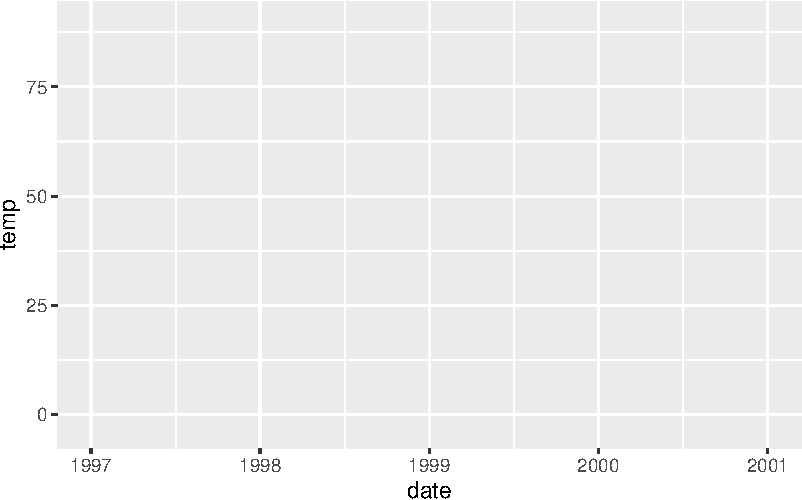
\includegraphics{ch3_files/figure-pdf/ggplot-1.pdf}

Ah, the reason only a panel is generated when executing this code is
because \texttt{\{ggplot2\}} lacks information on how we want to
visualize the data. We still need to specify a geometry!

In \texttt{\{ggplot2\}}, you can store the current \texttt{ggobject} in
a variable of your choosing, such as \texttt{g}. This allows you to
extend the \texttt{ggobject} later by adding additional layers, either
all at once or by assigning it to the same or another variable.

💡 \textbf{By using parentheses when assigning an object, the object
will be printed immediately. Instead of writing
\texttt{g\ \textless{}-\ ggplot(...)} followed by \texttt{g}, we can
simply write \texttt{(g\ \textless{}-\ ggplot(...))}.}

There's a wide array of geometries in \texttt{\{ggplot2\}}, often
referred to as \emph{geoms} because their function names typically start
with \texttt{geom\_}. You can find the full list of default geoms
\href{https://ggplot2.tidyverse.org/reference/}{here}, and there are
even more options available through extension packages, which you can
explore \href{https://exts.ggplot2.tidyverse.org/}{here}. To instruct
\texttt{\{ggplot2\}} on the style we want to use, we can, for example,
add \texttt{geom\_point()} to create a scatter plot:

\begin{Shaded}
\begin{Highlighting}[]
\NormalTok{g }\SpecialCharTok{+} \FunctionTok{geom\_point}\NormalTok{()}
\end{Highlighting}
\end{Shaded}

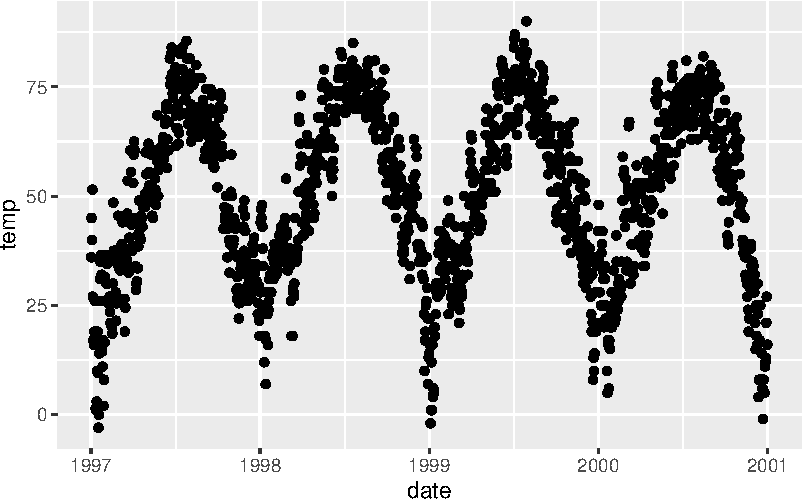
\includegraphics{ch3_files/figure-pdf/ggplot-default-1.pdf}

Great! However, this data could also be represented as a line plot
(although it might not be the optimal choice, but it's a common
practice). So, we can simply replace \texttt{geom\_point()} with
\texttt{geom\_line()} and boom!

\begin{Shaded}
\begin{Highlighting}[]
\NormalTok{g }\SpecialCharTok{+} \FunctionTok{geom\_line}\NormalTok{()}
\end{Highlighting}
\end{Shaded}

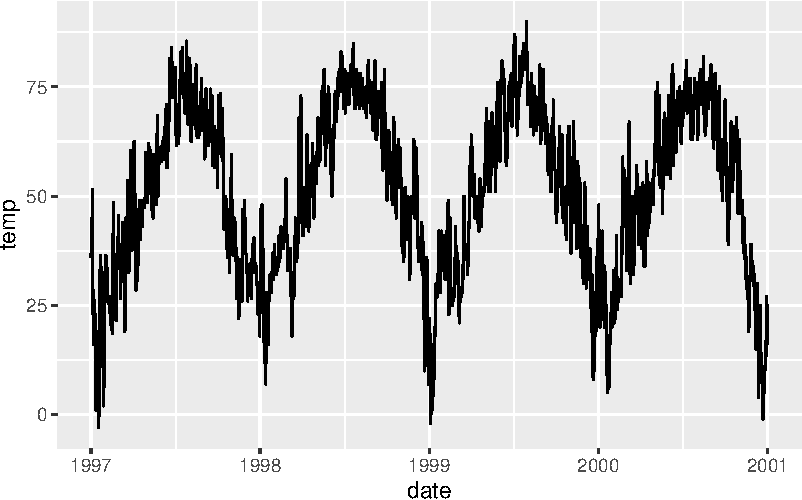
\includegraphics{ch3_files/figure-pdf/ggplot-default-line-1.pdf}

Indeed, one can combine multiple geometric layers, and this is where the
magic and fun truly begin!

\begin{Shaded}
\begin{Highlighting}[]
\NormalTok{g }\SpecialCharTok{+} \FunctionTok{geom\_line}\NormalTok{() }\SpecialCharTok{+} \FunctionTok{geom\_point}\NormalTok{()}
\end{Highlighting}
\end{Shaded}

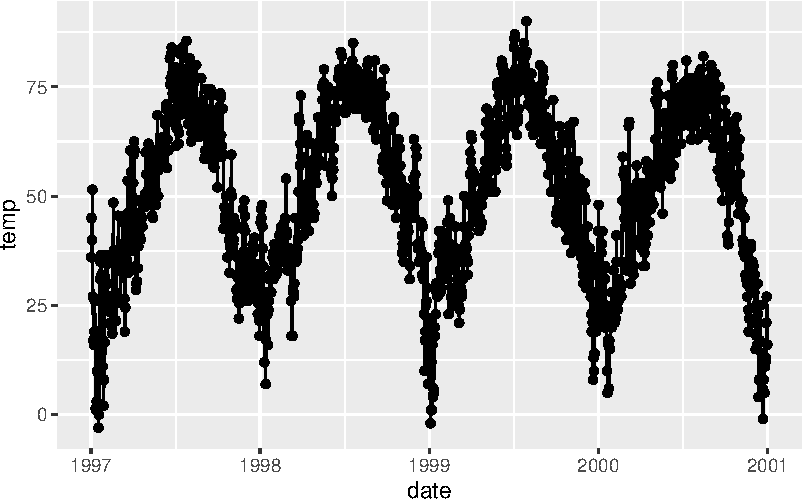
\includegraphics{ch3_files/figure-pdf/ggplot-default-line-point-1.pdf}

That's enough discussion on geometries for now. Don't worry, we'll dive
into various plot types at a later point, as outlined
\hyperref[charts]{here}.

\subsection{Change Properties of
Geometries}\label{change-properties-of-geometries}

Within the \texttt{geom\_*} command, you can already manipulate visual
aesthetics such as the color, shape, and size of your points. Let's
transform all points into large fire-red diamonds!

\begin{Shaded}
\begin{Highlighting}[]
\NormalTok{g }\SpecialCharTok{+} \FunctionTok{geom\_point}\NormalTok{(}\AttributeTok{color =} \StringTok{"firebrick"}\NormalTok{, }\AttributeTok{shape =} \StringTok{"diamond"}\NormalTok{, }\AttributeTok{size =} \DecValTok{2}\NormalTok{)}
\end{Highlighting}
\end{Shaded}

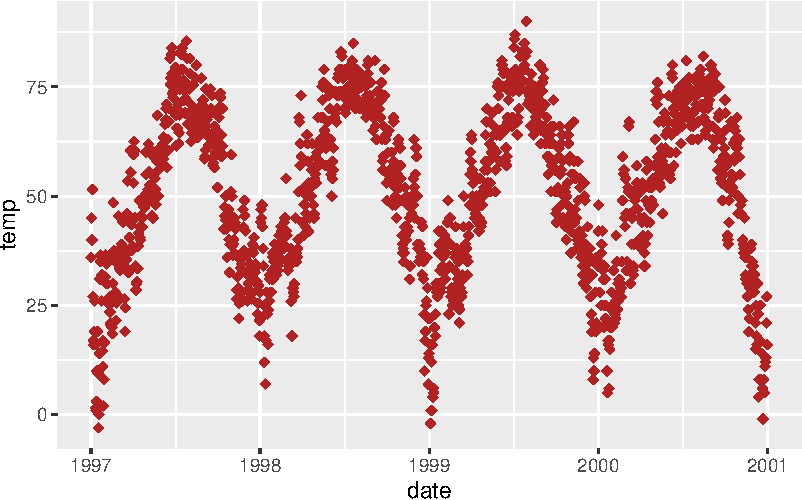
\includegraphics{ch3_files/figure-pdf/ggplot-default-col-size-shape-1.pdf}

💡 \textbf{\texttt{\{ggplot2\}} understands both \texttt{color} and
\texttt{colour} as well as the short version \texttt{col}.}

💁 You can utilize preset colors (a full list can be found
\href{http://www.stat.columbia.edu/~tzheng/files/Rcolor.pdf}{here}) or
\href{https://www.techopedia.com/definition/29788/color-hex-code}{hex
color codes}, both enclosed in quotes. Additionally, you can specify
RGB/RGBA colors using the \texttt{rgb()} function. Click to expand:

\begin{Shaded}
\begin{Highlighting}[]
\NormalTok{g }\SpecialCharTok{+} \FunctionTok{geom\_point}\NormalTok{(}\AttributeTok{color =} \StringTok{"\#b22222"}\NormalTok{, }\AttributeTok{shape =} \StringTok{"diamond"}\NormalTok{, }\AttributeTok{size =} \DecValTok{2}\NormalTok{)}
\NormalTok{g }\SpecialCharTok{+} \FunctionTok{geom\_point}\NormalTok{(}\AttributeTok{color =} \FunctionTok{rgb}\NormalTok{(}\DecValTok{178}\NormalTok{, }\DecValTok{34}\NormalTok{, }\DecValTok{34}\NormalTok{, }\AttributeTok{maxColorValue =} \DecValTok{255}\NormalTok{), }\AttributeTok{shape =} \StringTok{"diamond"}\NormalTok{, }\AttributeTok{size =} \DecValTok{2}\NormalTok{)}
\end{Highlighting}
\end{Shaded}

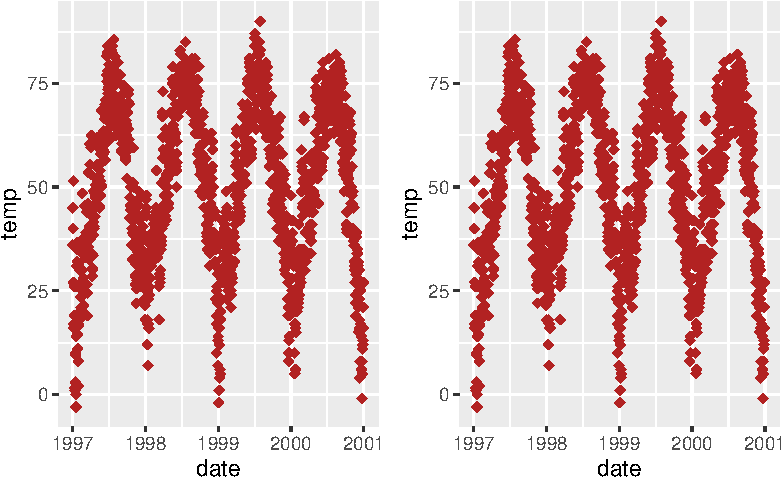
\includegraphics{ch3_files/figure-pdf/ggplot-default-col-size-hex-rgb-plot-1.pdf}

Each geom has its unique properties, referred to as \emph{arguments},
and the same argument might produce different effects depending on the
geom you're employing.

\begin{Shaded}
\begin{Highlighting}[]
\NormalTok{g }\SpecialCharTok{+} \FunctionTok{geom\_point}\NormalTok{(}\AttributeTok{color =} \StringTok{"firebrick"}\NormalTok{, }\AttributeTok{shape =} \StringTok{"diamond"}\NormalTok{, }\AttributeTok{size =} \DecValTok{2}\NormalTok{) }\SpecialCharTok{+}
    \FunctionTok{geom\_line}\NormalTok{(}\AttributeTok{color =} \StringTok{"firebrick"}\NormalTok{, }\AttributeTok{linetype =} \StringTok{"dotted"}\NormalTok{, }\AttributeTok{lwd =}\NormalTok{ .}\DecValTok{3}\NormalTok{)}
\end{Highlighting}
\end{Shaded}

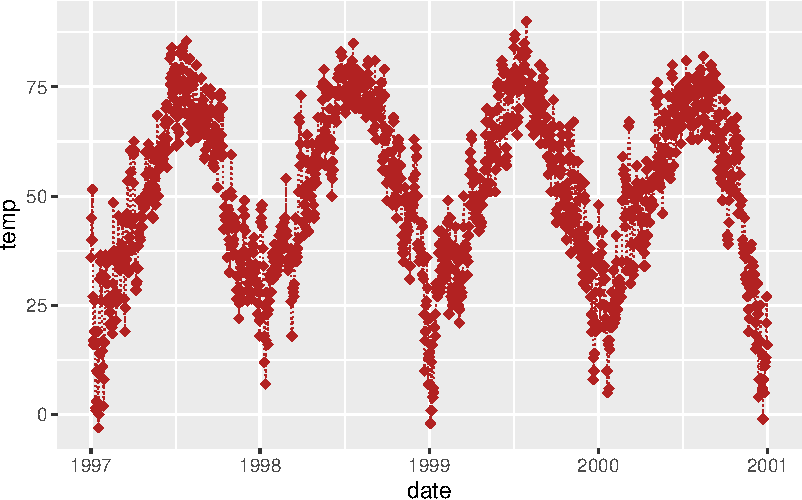
\includegraphics{ch3_files/figure-pdf/ggplot-default-line_col-size-shape-1.pdf}

\subsection{\texorpdfstring{Replace the default \texttt{ggplot2}
theme}{Replace the default ggplot2 theme}}\label{replace-the-default-ggplot2-theme}

To further demonstrate ggplot's versatility, let's enhance the
appearance by removing the default grayish \texttt{\{ggplot2\}} style
and setting a different built-in theme, such as \texttt{theme\_bw()}. By
using \texttt{theme\_set()}, all subsequent plots will adopt the same
black-and-white theme. This adjustment will notably enhance the
appearance of the red points!

\begin{Shaded}
\begin{Highlighting}[]
\FunctionTok{theme\_set}\NormalTok{(}\FunctionTok{theme\_bw}\NormalTok{())}

\NormalTok{g }\SpecialCharTok{+} \FunctionTok{geom\_point}\NormalTok{(}\AttributeTok{color =} \StringTok{"firebrick"}\NormalTok{)}
\end{Highlighting}
\end{Shaded}

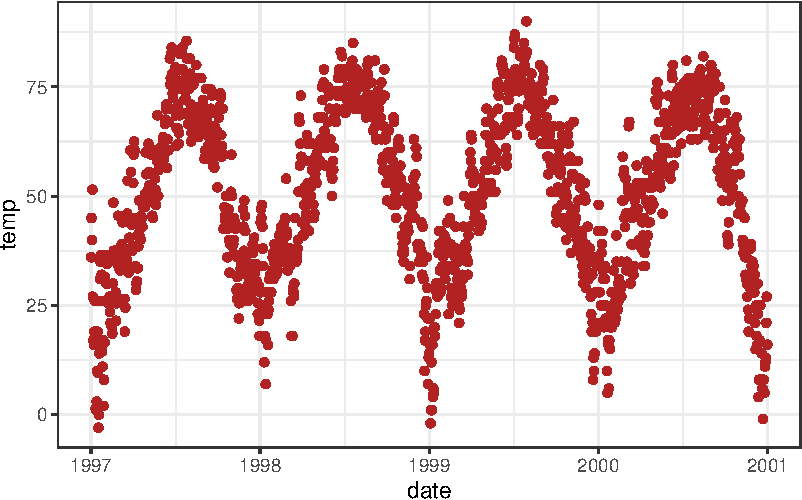
\includegraphics{ch3_files/figure-pdf/remove-gray-background-1.pdf}

For further details on using built-in themes and customizing themes,
refer to the section \hyperref[themes]{``Working with Themes''}.
Starting from the next chapter, we'll also utilize the \texttt{theme()}
function to customize specific elements of the theme.

💡 \textbf{\texttt{theme()} is a crucial command for manually adjusting
various theme elements such as texts, rectangles, and lines.}

To explore the numerous details of a ggplot theme that can be modified,
refer to the extensive list available
\href{https://ggplot2.tidyverse.org/reference/theme.html}{here}. Take
your time, as it's a comprehensive list!

\bookmarksetup{startatroot}

\chapter{Working with Axes}\label{axes}

\section{Change Axis Titles}\label{change-axis-titles}

To add clear and descriptive labels to the axes, we can utilize the
\texttt{labs()} function. This function allows us to provide a character
string for each label we wish to modify, such as \texttt{x} and
\texttt{y}:

\begin{Shaded}
\begin{Highlighting}[]
\FunctionTok{ggplot}\NormalTok{(chic, }\FunctionTok{aes}\NormalTok{(}\AttributeTok{x =}\NormalTok{ date, }\AttributeTok{y =}\NormalTok{ temp)) }\SpecialCharTok{+}
  \FunctionTok{geom\_point}\NormalTok{(}\AttributeTok{color =} \StringTok{"firebrick"}\NormalTok{) }\SpecialCharTok{+}
  \FunctionTok{labs}\NormalTok{(}\AttributeTok{x =} \StringTok{"Year"}\NormalTok{, }\AttributeTok{y =} \StringTok{"Temperature (°F)"}\NormalTok{)}
\end{Highlighting}
\end{Shaded}

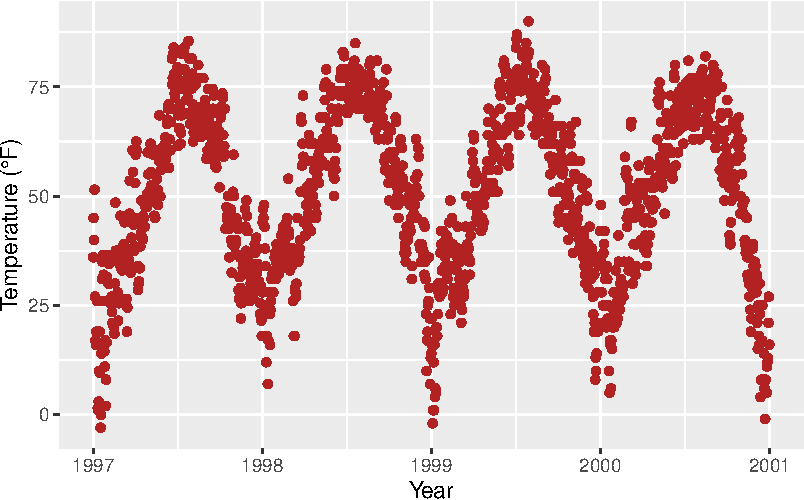
\includegraphics{ch4_files/figure-pdf/axis-labs-1.pdf}

💁 You also can add axis titles by using \texttt{xlab()} and
\texttt{ylab()}. Click to see example.

\begin{Shaded}
\begin{Highlighting}[]
\FunctionTok{ggplot}\NormalTok{(chic, }\FunctionTok{aes}\NormalTok{(}\AttributeTok{x =}\NormalTok{ date, }\AttributeTok{y =}\NormalTok{ temp)) }\SpecialCharTok{+}
  \FunctionTok{geom\_point}\NormalTok{(}\AttributeTok{color =} \StringTok{"firebrick"}\NormalTok{) }\SpecialCharTok{+}
  \FunctionTok{xlab}\NormalTok{(}\StringTok{"Year"}\NormalTok{) }\SpecialCharTok{+}
  \FunctionTok{ylab}\NormalTok{(}\StringTok{"Temperature (°F)"}\NormalTok{)}
\end{Highlighting}
\end{Shaded}

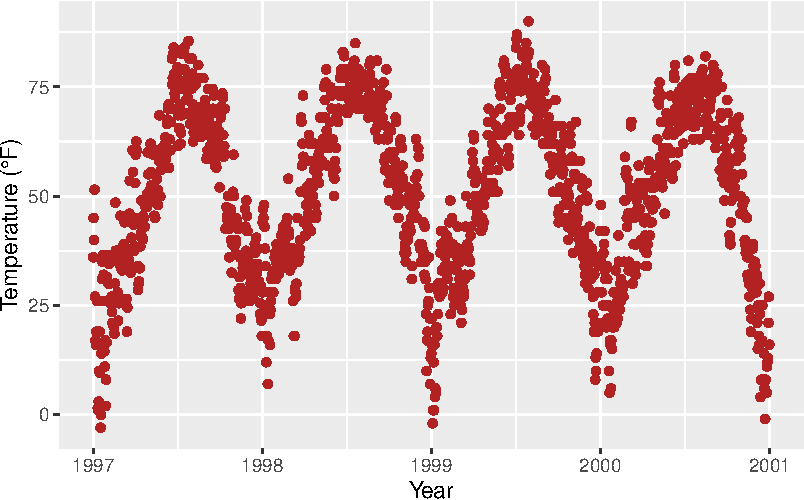
\includegraphics{ch4_files/figure-pdf/axis-labs-2-1.pdf}

Typically, you can specify symbols by directly adding the symbol itself
(e.g., ``°''). However, the code below also enables the addition of not
only symbols but also features like superscripts:

\begin{Shaded}
\begin{Highlighting}[]
\FunctionTok{ggplot}\NormalTok{(chic, }\FunctionTok{aes}\NormalTok{(}\AttributeTok{x =}\NormalTok{ date, }\AttributeTok{y =}\NormalTok{ temp)) }\SpecialCharTok{+}
  \FunctionTok{geom\_point}\NormalTok{(}\AttributeTok{color =} \StringTok{"firebrick"}\NormalTok{) }\SpecialCharTok{+}
  \FunctionTok{labs}\NormalTok{(}\AttributeTok{x =} \StringTok{"Year"}\NormalTok{, }\AttributeTok{y =} \FunctionTok{expression}\NormalTok{(}\FunctionTok{paste}\NormalTok{(}\StringTok{"Temperature ("}\NormalTok{, degree }\SpecialCharTok{\textasciitilde{}}\NormalTok{ F, }\StringTok{")"}\SpecialCharTok{\^{}}\StringTok{"(Hey, why should we use metric units?!)"}\NormalTok{)))}
\end{Highlighting}
\end{Shaded}

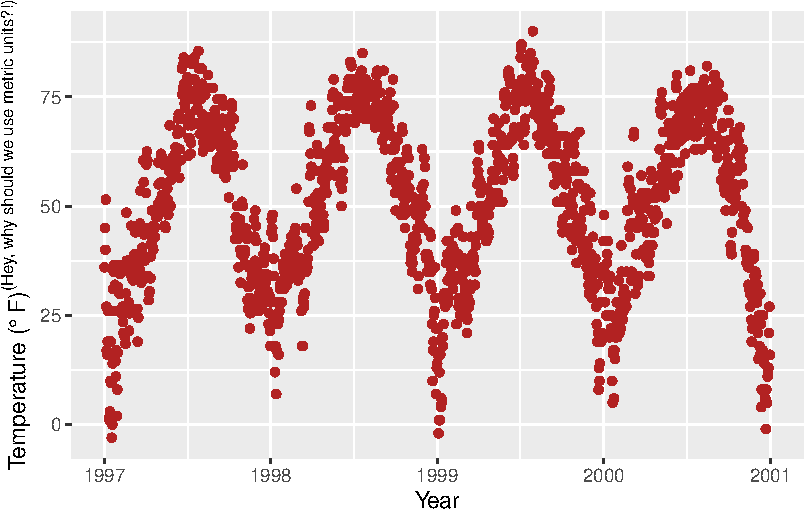
\includegraphics{ch4_files/figure-pdf/axis-labs-expression-1.pdf}

\section{Increase Space between Axis and Axis
Titles}\label{increase-space-between-axis-and-axis-titles}

\texttt{theme()} is a crucial command for adjusting specific theme
elements such as texts, titles, boxes, symbols, backgrounds, and more.
We'll be utilizing this command extensively! Initially, we'll focus on
modifying text elements. We can customize the properties of all text
elements or specific ones, such as axis titles, by overriding the
default \texttt{element\_text()} within the \texttt{theme()} call:

\begin{Shaded}
\begin{Highlighting}[]
\FunctionTok{ggplot}\NormalTok{(chic, }\FunctionTok{aes}\NormalTok{(}\AttributeTok{x =}\NormalTok{ date, }\AttributeTok{y =}\NormalTok{ temp)) }\SpecialCharTok{+}
  \FunctionTok{geom\_point}\NormalTok{(}\AttributeTok{color =} \StringTok{"firebrick"}\NormalTok{) }\SpecialCharTok{+}
  \FunctionTok{labs}\NormalTok{(}\AttributeTok{x =} \StringTok{"Year"}\NormalTok{, }\AttributeTok{y =} \StringTok{"Temperature (°F)"}\NormalTok{) }\SpecialCharTok{+}
  \FunctionTok{theme}\NormalTok{(}\AttributeTok{axis.title.x =} \FunctionTok{element\_text}\NormalTok{(}\AttributeTok{vjust =} \DecValTok{0}\NormalTok{, }\AttributeTok{size =} \DecValTok{15}\NormalTok{),}
        \AttributeTok{axis.title.y =} \FunctionTok{element\_text}\NormalTok{(}\AttributeTok{vjust =} \DecValTok{2}\NormalTok{, }\AttributeTok{size =} \DecValTok{15}\NormalTok{))}
\end{Highlighting}
\end{Shaded}

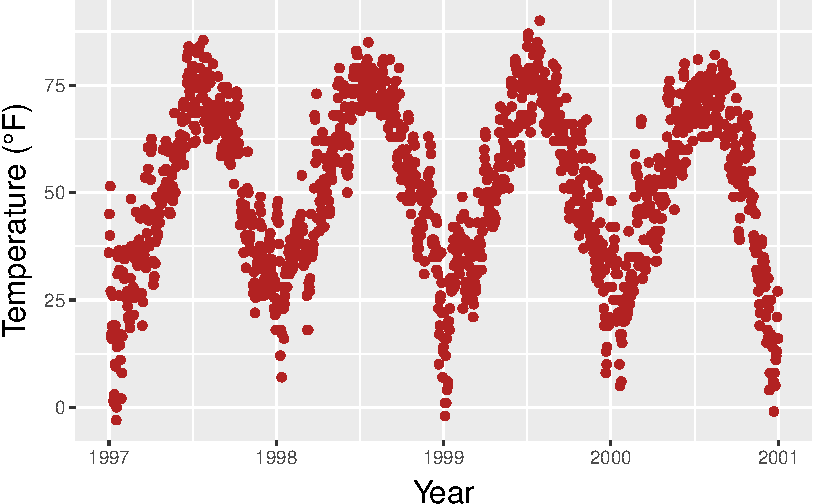
\includegraphics{ch4_files/figure-pdf/labs-move-away-vjust-1.pdf}

The \texttt{vjust} parameter controls vertical alignment and typically
ranges between 0 and 1, but you can also specify values outside that
range. It's worth noting that even when adjusting the position of the
axis title along the y-axis horizontally, we still need to specify
\texttt{vjust} (which is correct from the perspective of the label's
alignment). Additionally, you can modify the distance by specifying the
margin for both text elements:

\begin{Shaded}
\begin{Highlighting}[]
\FunctionTok{ggplot}\NormalTok{(chic, }\FunctionTok{aes}\NormalTok{(}\AttributeTok{x =}\NormalTok{ date, }\AttributeTok{y =}\NormalTok{ temp)) }\SpecialCharTok{+}
  \FunctionTok{geom\_point}\NormalTok{(}\AttributeTok{color =} \StringTok{"firebrick"}\NormalTok{) }\SpecialCharTok{+}
  \FunctionTok{labs}\NormalTok{(}\AttributeTok{x =} \StringTok{"Year"}\NormalTok{, }\AttributeTok{y =} \StringTok{"Temperature (°F)"}\NormalTok{) }\SpecialCharTok{+}
  \FunctionTok{theme}\NormalTok{(}\AttributeTok{axis.title.x =} \FunctionTok{element\_text}\NormalTok{(}\AttributeTok{margin =} \FunctionTok{margin}\NormalTok{(}\AttributeTok{t =} \DecValTok{10}\NormalTok{), }\AttributeTok{size =} \DecValTok{15}\NormalTok{),}
        \AttributeTok{axis.title.y =} \FunctionTok{element\_text}\NormalTok{(}\AttributeTok{margin =} \FunctionTok{margin}\NormalTok{(}\AttributeTok{r =} \DecValTok{10}\NormalTok{), }\AttributeTok{size =} \DecValTok{15}\NormalTok{))}
\end{Highlighting}
\end{Shaded}

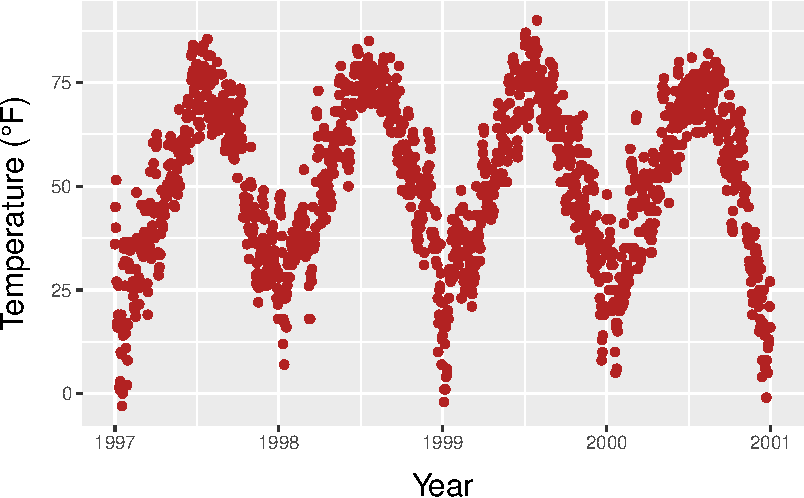
\includegraphics{ch4_files/figure-pdf/labs-move-away-margin-1.pdf}

The labels \texttt{t} and \texttt{r} within the \texttt{margin()} object
correspond to \emph{top} and \emph{right}, respectively. Alternatively,
you can specify all four margins using \texttt{margin(t,\ r,\ b,\ l)}.
It's important to note that we need to adjust the right margin to modify
the space on the y-axis, not the bottom margin.

💡 \textbf{A helpful mnemonic for remembering the order of the margin
sides is ``\emph{t}-\emph{r}-ou-\emph{b}-\emph{l}-e''.}

\section{Change Aesthetics of Axis
Titles}\label{change-aesthetics-of-axis-titles}

Once more, we utilize the \texttt{theme()} function to modify the
\texttt{axis.title} element and/or its subordinated elements,
\texttt{axis.title.x} and \texttt{axis.title.y}. Within the
\texttt{element\_text()} function, we can override defaults for
properties such as \texttt{size}, \texttt{color}, and \texttt{face}:

\begin{Shaded}
\begin{Highlighting}[]
\FunctionTok{ggplot}\NormalTok{(chic, }\FunctionTok{aes}\NormalTok{(}\AttributeTok{x =}\NormalTok{ date, }\AttributeTok{y =}\NormalTok{ temp)) }\SpecialCharTok{+}
  \FunctionTok{geom\_point}\NormalTok{(}\AttributeTok{color =} \StringTok{"firebrick"}\NormalTok{) }\SpecialCharTok{+}
  \FunctionTok{labs}\NormalTok{(}\AttributeTok{x =} \StringTok{"Year"}\NormalTok{, }\AttributeTok{y =} \StringTok{"Temperature (°F)"}\NormalTok{) }\SpecialCharTok{+}
  \FunctionTok{theme}\NormalTok{(}\AttributeTok{axis.title =} \FunctionTok{element\_text}\NormalTok{(}\AttributeTok{size =} \DecValTok{15}\NormalTok{, }\AttributeTok{color =} \StringTok{"firebrick"}\NormalTok{,}
                                  \AttributeTok{face =} \StringTok{"italic"}\NormalTok{))}
\end{Highlighting}
\end{Shaded}

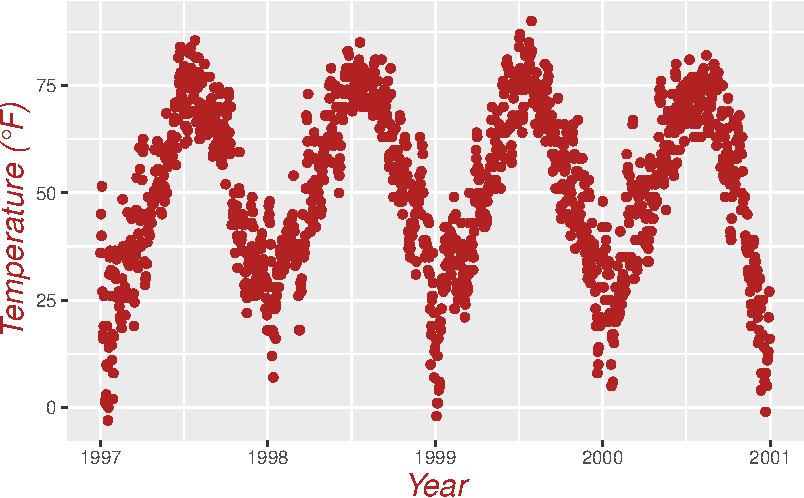
\includegraphics{ch4_files/figure-pdf/labs-color-axes-1-1.pdf}

The \texttt{face} argument can be used to make the font \texttt{bold} or
\texttt{italic} or even \texttt{bold.italic}.

\begin{Shaded}
\begin{Highlighting}[]
\FunctionTok{ggplot}\NormalTok{(chic, }\FunctionTok{aes}\NormalTok{(}\AttributeTok{x =}\NormalTok{ date, }\AttributeTok{y =}\NormalTok{ temp)) }\SpecialCharTok{+}
  \FunctionTok{geom\_point}\NormalTok{(}\AttributeTok{color =} \StringTok{"firebrick"}\NormalTok{) }\SpecialCharTok{+}
  \FunctionTok{labs}\NormalTok{(}\AttributeTok{x =} \StringTok{"Year"}\NormalTok{, }\AttributeTok{y =} \StringTok{"Temperature (°F)"}\NormalTok{) }\SpecialCharTok{+}
  \FunctionTok{theme}\NormalTok{(}\AttributeTok{axis.title.x =} \FunctionTok{element\_text}\NormalTok{(}\AttributeTok{color =} \StringTok{"sienna"}\NormalTok{, }\AttributeTok{size =} \DecValTok{15}\NormalTok{),}
        \AttributeTok{axis.title.y =} \FunctionTok{element\_text}\NormalTok{(}\AttributeTok{color =} \StringTok{"orangered"}\NormalTok{, }\AttributeTok{size =} \DecValTok{15}\NormalTok{))}
\end{Highlighting}
\end{Shaded}

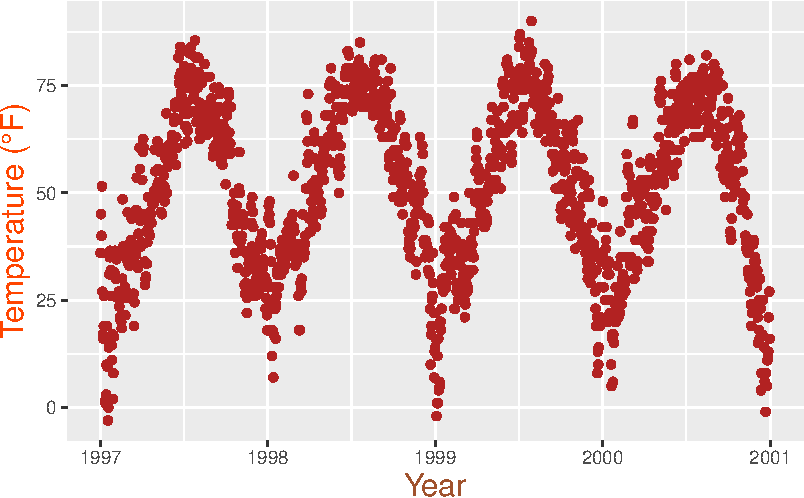
\includegraphics{ch4_files/figure-pdf/labs-color-axes-2-1.pdf}

💁 You could also employ a combination of \texttt{axis.title} and
\texttt{axis.title.y}, as \texttt{axis.title.x} inherits values from
\texttt{axis.title}. Expand to See the example below:

\begin{Shaded}
\begin{Highlighting}[]
\FunctionTok{ggplot}\NormalTok{(chic, }\FunctionTok{aes}\NormalTok{(}\AttributeTok{x =}\NormalTok{ date, }\AttributeTok{y =}\NormalTok{ temp)) }\SpecialCharTok{+}
  \FunctionTok{geom\_point}\NormalTok{(}\AttributeTok{color =} \StringTok{"firebrick"}\NormalTok{) }\SpecialCharTok{+}
  \FunctionTok{labs}\NormalTok{(}\AttributeTok{x =} \StringTok{"Year"}\NormalTok{, }\AttributeTok{y =} \StringTok{"Temperature (°F)"}\NormalTok{) }\SpecialCharTok{+}
  \FunctionTok{theme}\NormalTok{(}\AttributeTok{axis.title =} \FunctionTok{element\_text}\NormalTok{(}\AttributeTok{color =} \StringTok{"sienna"}\NormalTok{, }\AttributeTok{size =} \DecValTok{15}\NormalTok{),}
        \AttributeTok{axis.title.y =} \FunctionTok{element\_text}\NormalTok{(}\AttributeTok{color =} \StringTok{"orangered"}\NormalTok{, }\AttributeTok{size =} \DecValTok{15}\NormalTok{))}
\end{Highlighting}
\end{Shaded}

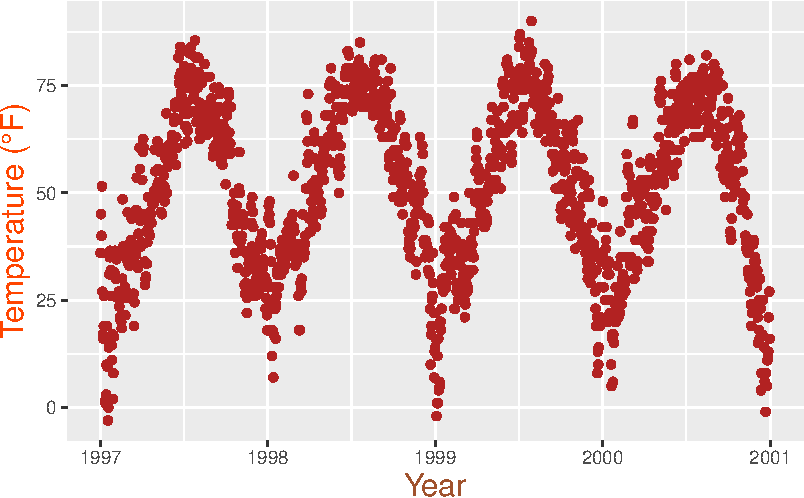
\includegraphics{ch4_files/figure-pdf/labs-color-axes-3-1.pdf}

You can adjust some properties for both axis titles simultaneously,
while modifying others exclusively for one axis or individual properties
for each axis title:

\begin{Shaded}
\begin{Highlighting}[]
\FunctionTok{ggplot}\NormalTok{(chic, }\FunctionTok{aes}\NormalTok{(}\AttributeTok{x =}\NormalTok{ date, }\AttributeTok{y =}\NormalTok{ temp)) }\SpecialCharTok{+}
  \FunctionTok{geom\_point}\NormalTok{(}\AttributeTok{color =} \StringTok{"firebrick"}\NormalTok{) }\SpecialCharTok{+}
  \FunctionTok{labs}\NormalTok{(}\AttributeTok{x =} \StringTok{"Year"}\NormalTok{, }\AttributeTok{y =} \StringTok{"Temperature (°F)"}\NormalTok{) }\SpecialCharTok{+}
  \FunctionTok{theme}\NormalTok{(}\AttributeTok{axis.title =} \FunctionTok{element\_text}\NormalTok{(}\AttributeTok{color =} \StringTok{"sienna"}\NormalTok{, }\AttributeTok{size =} \DecValTok{15}\NormalTok{, }\AttributeTok{face =} \StringTok{"bold"}\NormalTok{),}
        \AttributeTok{axis.title.y =} \FunctionTok{element\_text}\NormalTok{(}\AttributeTok{face =} \StringTok{"bold.italic"}\NormalTok{))}
\end{Highlighting}
\end{Shaded}

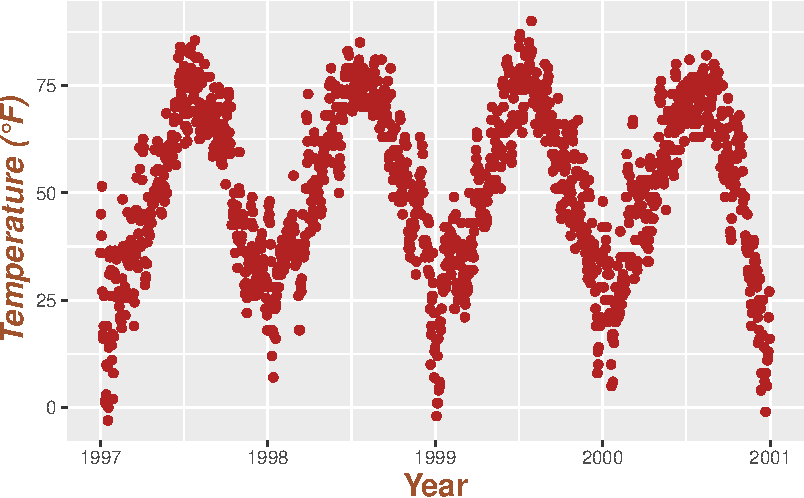
\includegraphics{ch4_files/figure-pdf/labs-color-axes-4-1.pdf}

\section{Change Aesthetics of Axis
Text}\label{change-aesthetics-of-axis-text}

Likewise, you can alter the appearance of the axis text (i.e., the
numbers) by utilizing \texttt{axis.text} and/or its subordinated
elements, \texttt{axis.text.x} and \texttt{axis.text.y}:

\begin{Shaded}
\begin{Highlighting}[]
\FunctionTok{ggplot}\NormalTok{(chic, }\FunctionTok{aes}\NormalTok{(}\AttributeTok{x =}\NormalTok{ date, }\AttributeTok{y =}\NormalTok{ temp)) }\SpecialCharTok{+}
  \FunctionTok{geom\_point}\NormalTok{(}\AttributeTok{color =} \StringTok{"firebrick"}\NormalTok{) }\SpecialCharTok{+}
  \FunctionTok{labs}\NormalTok{(}\AttributeTok{x =} \StringTok{"Year"}\NormalTok{, }\AttributeTok{y =} \StringTok{"Temperature (°F)"}\NormalTok{) }\SpecialCharTok{+}
  \FunctionTok{theme}\NormalTok{(}\AttributeTok{axis.text =} \FunctionTok{element\_text}\NormalTok{(}\AttributeTok{color =} \StringTok{"dodgerblue"}\NormalTok{, }\AttributeTok{size =} \DecValTok{12}\NormalTok{),}
        \AttributeTok{axis.text.x =} \FunctionTok{element\_text}\NormalTok{(}\AttributeTok{face =} \StringTok{"italic"}\NormalTok{))}
\end{Highlighting}
\end{Shaded}

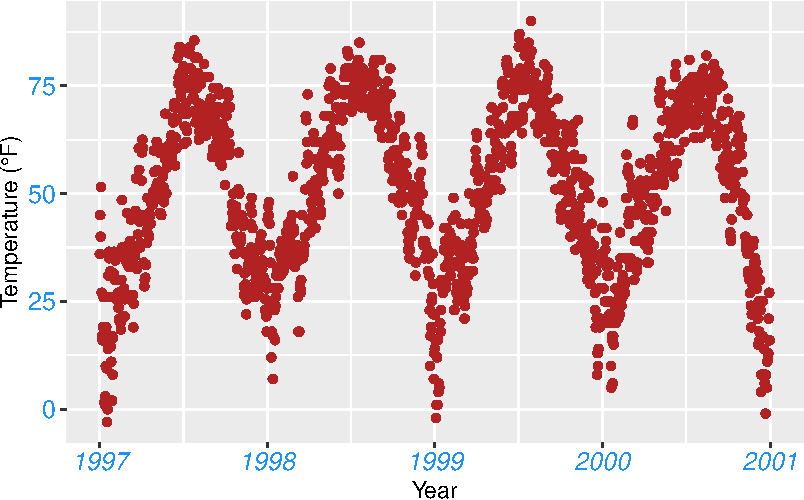
\includegraphics{ch4_files/figure-pdf/labs-color-axes-text-1.pdf}

\section{Rotate Axis Text}\label{rotate-axis-text}

You can rotate any text elements by specifying an \texttt{angle}.
Subsequently, you can adjust the position of the text horizontally (0 =
left, 1 = right) and vertically (0 = top, 1 = bottom) using
\texttt{hjust} and \texttt{vjust}:

\begin{Shaded}
\begin{Highlighting}[]
\FunctionTok{ggplot}\NormalTok{(chic, }\FunctionTok{aes}\NormalTok{(}\AttributeTok{x =}\NormalTok{ date, }\AttributeTok{y =}\NormalTok{ temp)) }\SpecialCharTok{+}
  \FunctionTok{geom\_point}\NormalTok{(}\AttributeTok{color =} \StringTok{"firebrick"}\NormalTok{) }\SpecialCharTok{+}
  \FunctionTok{labs}\NormalTok{(}\AttributeTok{x =} \StringTok{"Year"}\NormalTok{, }\AttributeTok{y =} \StringTok{"Temperature (°F)"}\NormalTok{) }\SpecialCharTok{+}
  \FunctionTok{theme}\NormalTok{(}\AttributeTok{axis.text.x =} \FunctionTok{element\_text}\NormalTok{(}\AttributeTok{angle =} \DecValTok{50}\NormalTok{, }\AttributeTok{vjust =} \DecValTok{1}\NormalTok{, }\AttributeTok{hjust =} \DecValTok{1}\NormalTok{, }\AttributeTok{size =} \DecValTok{12}\NormalTok{))}
\end{Highlighting}
\end{Shaded}

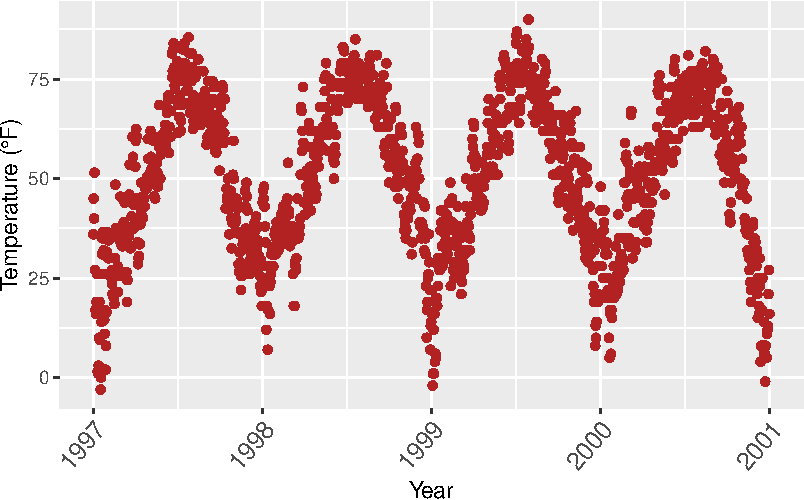
\includegraphics{ch4_files/figure-pdf/axis-text-1.pdf}

\section{Removing Axis Text \& Ticks}\label{removing-axis-text-ticks}

There might be rare occasions where you need to remove axis text and
ticks. Here's how you can achieve it:

\begin{Shaded}
\begin{Highlighting}[]
\FunctionTok{ggplot}\NormalTok{(chic, }\FunctionTok{aes}\NormalTok{(}\AttributeTok{x =}\NormalTok{ date, }\AttributeTok{y =}\NormalTok{ temp)) }\SpecialCharTok{+}
  \FunctionTok{geom\_point}\NormalTok{(}\AttributeTok{color =} \StringTok{"firebrick"}\NormalTok{) }\SpecialCharTok{+}
  \FunctionTok{labs}\NormalTok{(}\AttributeTok{x =} \StringTok{"Year"}\NormalTok{, }\AttributeTok{y =} \StringTok{"Temperature (°F)"}\NormalTok{) }\SpecialCharTok{+}
  \FunctionTok{theme}\NormalTok{(}\AttributeTok{axis.ticks.y =} \FunctionTok{element\_blank}\NormalTok{(),}
        \AttributeTok{axis.text.y =} \FunctionTok{element\_blank}\NormalTok{())}
\end{Highlighting}
\end{Shaded}

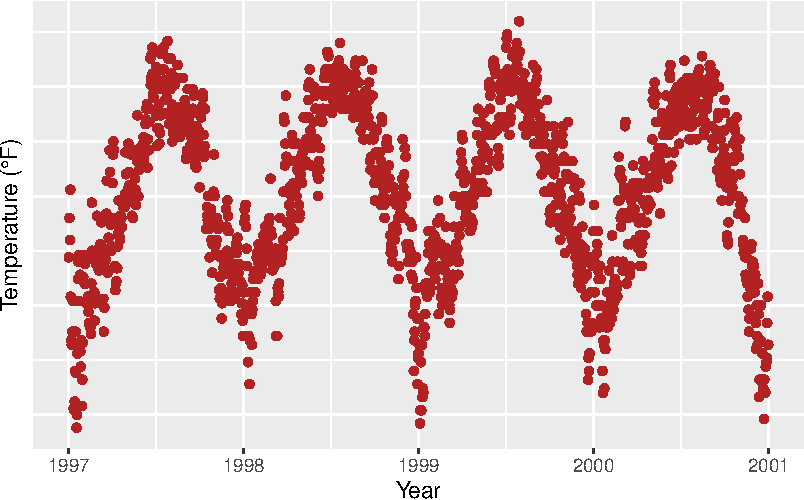
\includegraphics{ch4_files/figure-pdf/axis-no-labs-1.pdf}

I've introduced three theme elements---text, lines, and rectangles---but
there's actually one more: \texttt{element\_blank()}, which removes the
element entirely. However, it's not considered an official element like
the others.

💡 \textbf{If you wish to remove a theme element entirely, you can
always use \texttt{element\_blank()}.}

\section{Removing Axis Titles}\label{removing-axis-titles}

We can use \texttt{theme\_blank()}, but it's much simpler to just omit
the label in the \texttt{labs()} (or \texttt{xlab()}) call:

\begin{Shaded}
\begin{Highlighting}[]
\FunctionTok{ggplot}\NormalTok{(chic, }\FunctionTok{aes}\NormalTok{(}\AttributeTok{x =}\NormalTok{ date, }\AttributeTok{y =}\NormalTok{ temp)) }\SpecialCharTok{+}
  \FunctionTok{geom\_point}\NormalTok{(}\AttributeTok{color =} \StringTok{"firebrick"}\NormalTok{) }\SpecialCharTok{+}
  \FunctionTok{labs}\NormalTok{(}\AttributeTok{x =} \ConstantTok{NULL}\NormalTok{, }\AttributeTok{y =} \StringTok{""}\NormalTok{)}
\end{Highlighting}
\end{Shaded}

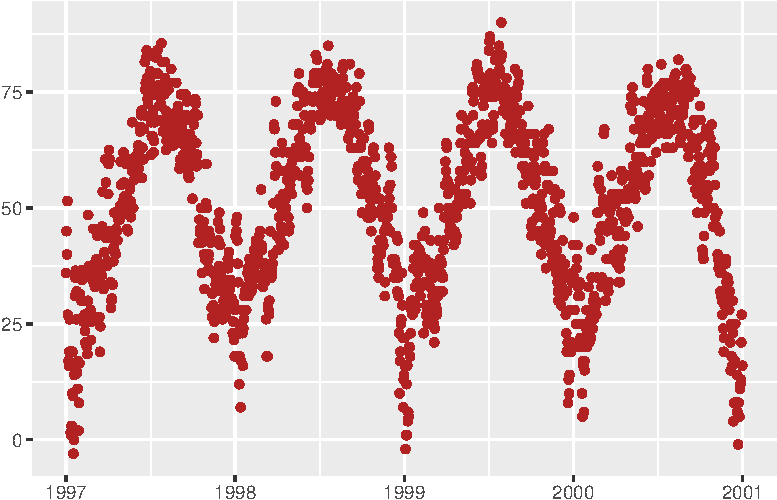
\includegraphics{ch4_files/figure-pdf/axis-no-title-1.pdf}

💡 \textbf{Note that \texttt{NULL} removes the element (similarly to
\texttt{element\_blank()}), while empty quotes \texttt{""} will keep the
spacing for the axis title but print nothing.}

\section{Limiting Axis Range}\label{limiting-axis-range}

Occasionally, you may want to focus on a specific range of your data
without altering the dataset itself. You can accomplish this with ease:

\begin{Shaded}
\begin{Highlighting}[]
\FunctionTok{ggplot}\NormalTok{(chic, }\FunctionTok{aes}\NormalTok{(}\AttributeTok{x =}\NormalTok{ date, }\AttributeTok{y =}\NormalTok{ temp)) }\SpecialCharTok{+}
  \FunctionTok{geom\_point}\NormalTok{(}\AttributeTok{color =} \StringTok{"firebrick"}\NormalTok{) }\SpecialCharTok{+}
  \FunctionTok{labs}\NormalTok{(}\AttributeTok{x =} \StringTok{"Year"}\NormalTok{, }\AttributeTok{y =} \StringTok{"Temperature (°F)"}\NormalTok{) }\SpecialCharTok{+}
  \FunctionTok{ylim}\NormalTok{(}\FunctionTok{c}\NormalTok{(}\DecValTok{0}\NormalTok{, }\DecValTok{50}\NormalTok{))}
\end{Highlighting}
\end{Shaded}

\begin{verbatim}
Warning: Removed 777 rows containing missing values or values outside the scale range
(`geom_point()`).
\end{verbatim}

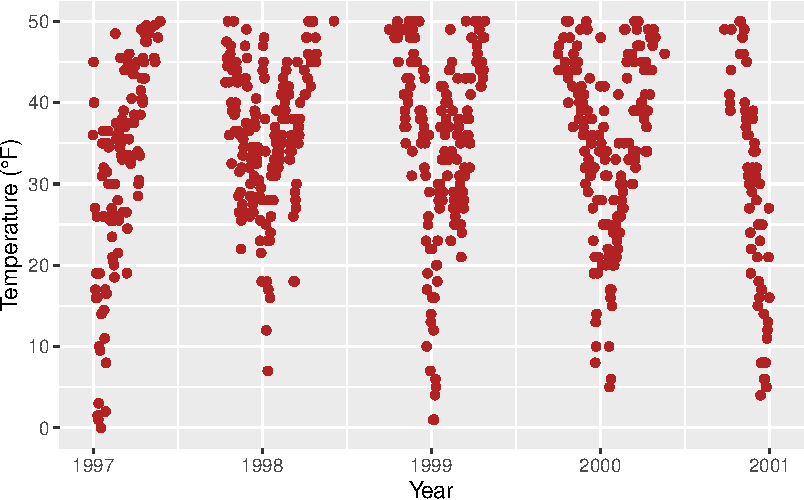
\includegraphics{ch4_files/figure-pdf/axis-limit-1.pdf}

Alternatively, you can utilize
\texttt{scale\_y\_continuous(limits\ =\ c(0,\ 50))} or
\texttt{coord\_cartesian(ylim\ =\ c(0,\ 50))}. The former removes all
data points outside the specified range, while the latter adjusts the
visible area, similar to \texttt{ylim(c(0,\ 50))}. At first glance, it
may seem that both approaches yield the same result. However, there is
an important distinction---compare the following two plots:

\begin{verbatim}
Warning: Removed 777 rows containing missing values or values outside the scale range
(`geom_point()`).
\end{verbatim}

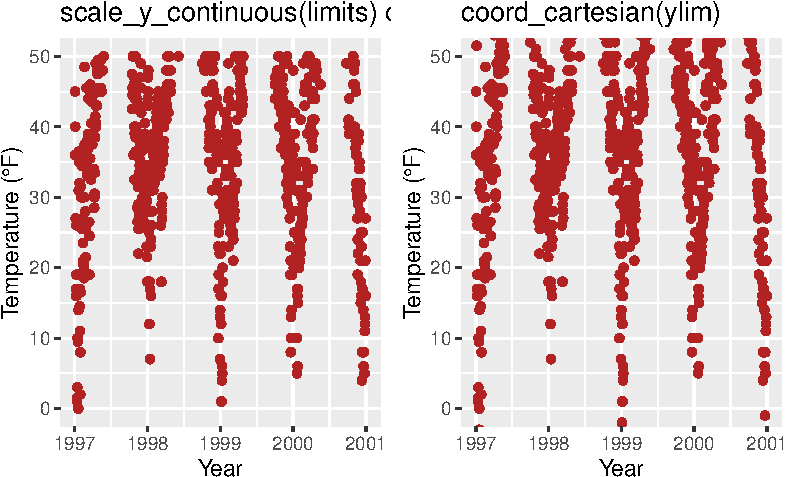
\includegraphics{ch4_files/figure-pdf/axis-limit-comp-1.pdf}

You may have noticed that on the left, there is some empty buffer around
your y limits, while on the right, points are plotted right up to the
border and even beyond. This effectively illustrates the concept of
subsetting (left) versus zooming (right). To demonstrate why this
distinction is significant, let's examine a different chart type: a box
plot.

\begin{verbatim}
Warning: Removed 777 rows containing non-finite outside the scale range
(`stat_boxplot()`).
\end{verbatim}

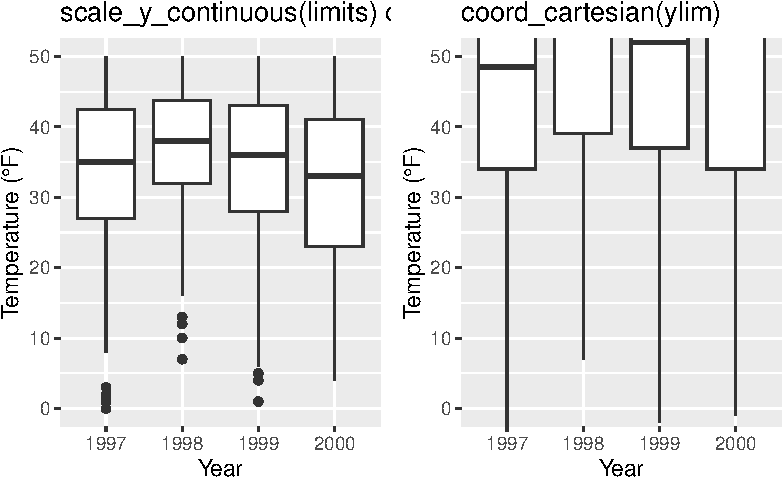
\includegraphics{ch4_files/figure-pdf/axis-limit-comp-box-1.pdf}

Indeed, because \texttt{scale\_x\textbar{}y\_continuous()} subsets the
data first, we obtain completely different (and potentially incorrect,
especially if this was not our intention) estimates for the box plots!
This realization highlights the importance of ensuring data integrity
throughout the plotting process. It's crucial to avoid inadvertently
manipulating the data while plotting, as it could lead to inaccurate
summary statistics reported in your report, paper, or thesis.

\section{Forcing Plot to Start at
Origin}\label{forcing-plot-to-start-at-origin}

Related to that, you can instruct R to plot the graph starting at the
origin:

\begin{Shaded}
\begin{Highlighting}[]
\NormalTok{chic\_high }\OtherTok{\textless{}{-}}\NormalTok{ dplyr}\SpecialCharTok{::}\FunctionTok{filter}\NormalTok{(chic, temp }\SpecialCharTok{\textgreater{}} \DecValTok{25}\NormalTok{, o3 }\SpecialCharTok{\textgreater{}} \DecValTok{20}\NormalTok{)}

\FunctionTok{ggplot}\NormalTok{(chic\_high, }\FunctionTok{aes}\NormalTok{(}\AttributeTok{x =}\NormalTok{ temp, }\AttributeTok{y =}\NormalTok{ o3)) }\SpecialCharTok{+}
  \FunctionTok{geom\_point}\NormalTok{(}\AttributeTok{color =} \StringTok{"darkcyan"}\NormalTok{) }\SpecialCharTok{+}
  \FunctionTok{labs}\NormalTok{(}\AttributeTok{x =} \StringTok{"Temperature higher than 25°F"}\NormalTok{,}
       \AttributeTok{y =} \StringTok{"Ozone higher than 20 ppb"}\NormalTok{) }\SpecialCharTok{+}
  \FunctionTok{expand\_limits}\NormalTok{(}\AttributeTok{x =} \DecValTok{0}\NormalTok{, }\AttributeTok{y =} \DecValTok{0}\NormalTok{)}
\end{Highlighting}
\end{Shaded}

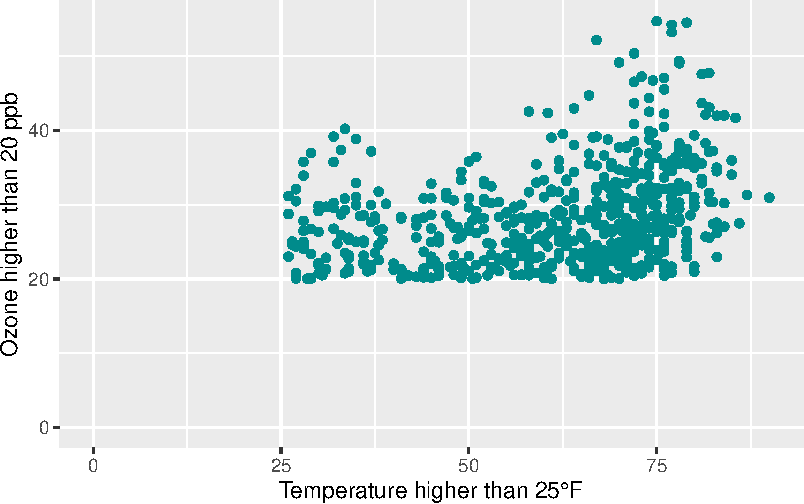
\includegraphics{ch4_files/figure-pdf/origin-1.pdf}

💁 Using
\texttt{coord\_cartesian(xlim\ =\ c(0,\ NA),\ ylim\ =\ c(0,\ NA))} will
produce the same result. CLICK to See the example below:

\begin{Shaded}
\begin{Highlighting}[]
\NormalTok{chic\_high }\OtherTok{\textless{}{-}}\NormalTok{ dplyr}\SpecialCharTok{::}\FunctionTok{filter}\NormalTok{(chic, temp }\SpecialCharTok{\textgreater{}} \DecValTok{25}\NormalTok{, o3 }\SpecialCharTok{\textgreater{}} \DecValTok{20}\NormalTok{)}

\FunctionTok{ggplot}\NormalTok{(chic\_high, }\FunctionTok{aes}\NormalTok{(}\AttributeTok{x =}\NormalTok{ temp, }\AttributeTok{y =}\NormalTok{ o3)) }\SpecialCharTok{+}
  \FunctionTok{geom\_point}\NormalTok{(}\AttributeTok{color =} \StringTok{"darkcyan"}\NormalTok{) }\SpecialCharTok{+}
  \FunctionTok{labs}\NormalTok{(}\AttributeTok{x =} \StringTok{"Temperature higher than 25°F"}\NormalTok{,}
       \AttributeTok{y =} \StringTok{"Ozone higher than 20 ppb"}\NormalTok{) }\SpecialCharTok{+}
  \FunctionTok{coord\_cartesian}\NormalTok{(}\AttributeTok{xlim =} \FunctionTok{c}\NormalTok{(}\DecValTok{0}\NormalTok{, }\ConstantTok{NA}\NormalTok{), }\AttributeTok{ylim =} \FunctionTok{c}\NormalTok{(}\DecValTok{0}\NormalTok{, }\ConstantTok{NA}\NormalTok{))}
\end{Highlighting}
\end{Shaded}

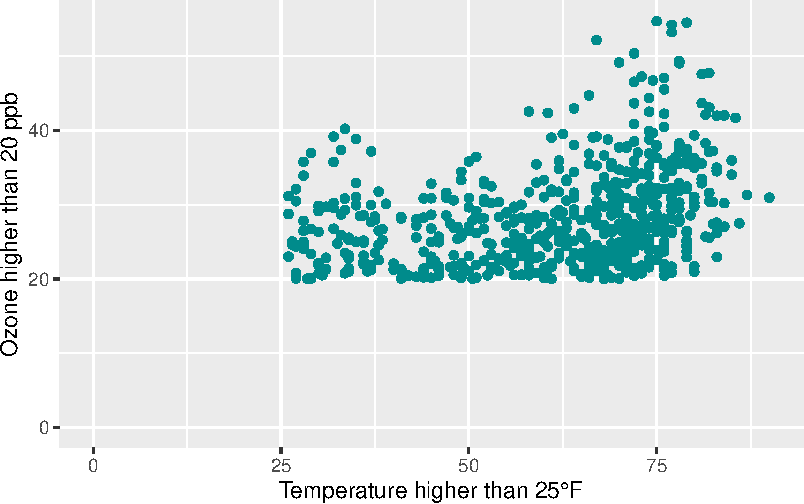
\includegraphics{ch4_files/figure-pdf/origin-coord-1.pdf}

But we can also ensure that it \emph{truly} starts at the origin!

\begin{Shaded}
\begin{Highlighting}[]
\FunctionTok{ggplot}\NormalTok{(chic\_high, }\FunctionTok{aes}\NormalTok{(}\AttributeTok{x =}\NormalTok{ temp, }\AttributeTok{y =}\NormalTok{ o3)) }\SpecialCharTok{+}
  \FunctionTok{geom\_point}\NormalTok{(}\AttributeTok{color =} \StringTok{"darkcyan"}\NormalTok{) }\SpecialCharTok{+}
  \FunctionTok{labs}\NormalTok{(}\AttributeTok{x =} \StringTok{"Temperature higher than 25°F"}\NormalTok{,}
       \AttributeTok{y =} \StringTok{"Ozone higher than 20 ppb"}\NormalTok{) }\SpecialCharTok{+}
  \FunctionTok{expand\_limits}\NormalTok{(}\AttributeTok{x =} \DecValTok{0}\NormalTok{, }\AttributeTok{y =} \DecValTok{0}\NormalTok{) }\SpecialCharTok{+}
  \FunctionTok{coord\_cartesian}\NormalTok{(}\AttributeTok{expand =} \ConstantTok{FALSE}\NormalTok{, }\AttributeTok{clip =} \StringTok{"off"}\NormalTok{)}
\end{Highlighting}
\end{Shaded}

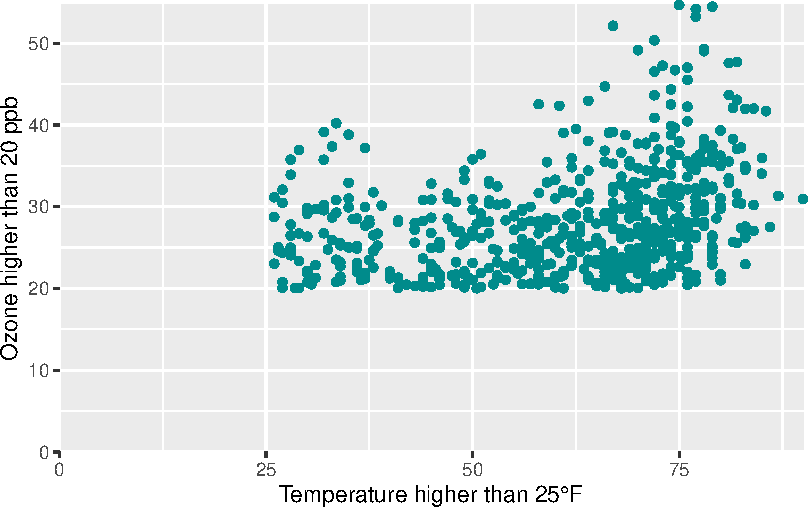
\includegraphics{ch4_files/figure-pdf/origin-force-1.pdf}

💡 \textbf{The \texttt{clip\ =\ "off"} argument in any coordinate
system, always starting with \texttt{coord\_*}, enables drawing outside
of the panel area.}

Here, I invoke it to ensure that the tick marks at \texttt{c(0,\ 0)}
remain intact and are not truncated. For further insights, refer to the
\href{https://twitter.com/clauswilke/status/991542952802619392?lang=en}{Twitter
thread by Claus Wilke}.

\section{Axes with Same Scaling}\label{axes-with-same-scaling}

For demonstration purposes, let's plot temperature against temperature
with some random noise. The \texttt{coord\_equal()} function provides a
coordinate system with a specified ratio, representing the number of
units on the y-axis equivalent to one unit on the x-axis. By default,
\texttt{ratio\ =\ 1} ensures that one unit on the x-axis is the same
length as one unit on the y-axis:

\begin{Shaded}
\begin{Highlighting}[]
\FunctionTok{ggplot}\NormalTok{(chic, }\FunctionTok{aes}\NormalTok{(}\AttributeTok{x =}\NormalTok{ temp, }\AttributeTok{y =}\NormalTok{ temp }\SpecialCharTok{+} \FunctionTok{rnorm}\NormalTok{(}\FunctionTok{nrow}\NormalTok{(chic), }\AttributeTok{sd =} \DecValTok{20}\NormalTok{))) }\SpecialCharTok{+}
  \FunctionTok{geom\_point}\NormalTok{(}\AttributeTok{color =} \StringTok{"sienna"}\NormalTok{) }\SpecialCharTok{+}
  \FunctionTok{labs}\NormalTok{(}\AttributeTok{x =} \StringTok{"Temperature (°F)"}\NormalTok{, }\AttributeTok{y =} \StringTok{"Temperature (°F) + random noise"}\NormalTok{) }\SpecialCharTok{+}
  \FunctionTok{xlim}\NormalTok{(}\FunctionTok{c}\NormalTok{(}\DecValTok{0}\NormalTok{, }\DecValTok{100}\NormalTok{)) }\SpecialCharTok{+} \FunctionTok{ylim}\NormalTok{(}\FunctionTok{c}\NormalTok{(}\DecValTok{0}\NormalTok{, }\DecValTok{150}\NormalTok{)) }\SpecialCharTok{+}
  \FunctionTok{coord\_fixed}\NormalTok{()}
\end{Highlighting}
\end{Shaded}

\begin{verbatim}
Warning: Removed 53 rows containing missing values or values outside the scale range
(`geom_point()`).
\end{verbatim}

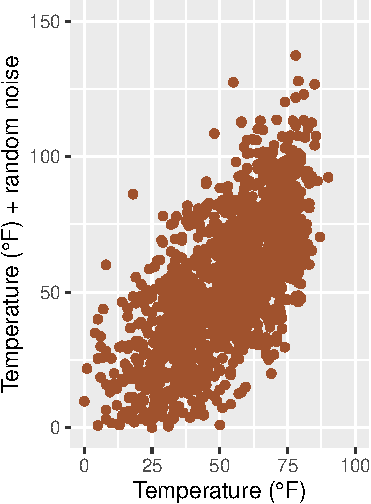
\includegraphics{ch4_files/figure-pdf/axes-equal-1.pdf}

Ratios higher than one result in units on the y-axis being longer than
units on the x-axis, while ratios lower than one have the opposite
effect:

\begin{Shaded}
\begin{Highlighting}[]
\FunctionTok{ggplot}\NormalTok{(chic, }\FunctionTok{aes}\NormalTok{(}\AttributeTok{x =}\NormalTok{ temp, }\AttributeTok{y =}\NormalTok{ temp }\SpecialCharTok{+} \FunctionTok{rnorm}\NormalTok{(}\FunctionTok{nrow}\NormalTok{(chic), }\AttributeTok{sd =} \DecValTok{20}\NormalTok{))) }\SpecialCharTok{+}
  \FunctionTok{geom\_point}\NormalTok{(}\AttributeTok{color =} \StringTok{"sienna"}\NormalTok{) }\SpecialCharTok{+}
  \FunctionTok{labs}\NormalTok{(}\AttributeTok{x =} \StringTok{"Temperature (°F)"}\NormalTok{, }\AttributeTok{y =} \StringTok{"Temperature (°F) + random noise"}\NormalTok{) }\SpecialCharTok{+}
  \FunctionTok{xlim}\NormalTok{(}\FunctionTok{c}\NormalTok{(}\DecValTok{0}\NormalTok{, }\DecValTok{100}\NormalTok{)) }\SpecialCharTok{+} \FunctionTok{ylim}\NormalTok{(}\FunctionTok{c}\NormalTok{(}\DecValTok{0}\NormalTok{, }\DecValTok{150}\NormalTok{)) }\SpecialCharTok{+}
  \FunctionTok{coord\_fixed}\NormalTok{(}\AttributeTok{ratio =} \DecValTok{1}\SpecialCharTok{/}\DecValTok{5}\NormalTok{)}
\end{Highlighting}
\end{Shaded}

\begin{verbatim}
Warning: Removed 49 rows containing missing values or values outside the scale range
(`geom_point()`).
\end{verbatim}

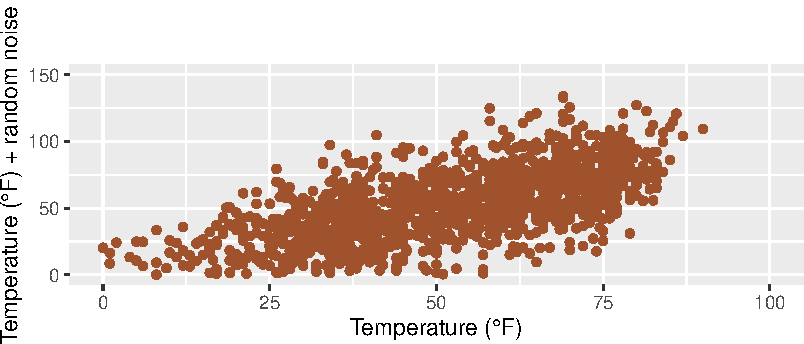
\includegraphics{ch4_files/figure-pdf/axes-fixed-2-1.pdf}

\section{Using a Function to Alter
Labels}\label{using-a-function-to-alter-labels}

Occasionally, it's useful to slightly modify your labels, such as adding
units or percent signs, without altering your underlying data. You can
achieve this using a function:

\begin{Shaded}
\begin{Highlighting}[]
\FunctionTok{ggplot}\NormalTok{(chic, }\FunctionTok{aes}\NormalTok{(}\AttributeTok{x =}\NormalTok{ date, }\AttributeTok{y =}\NormalTok{ temp)) }\SpecialCharTok{+}
  \FunctionTok{geom\_point}\NormalTok{(}\AttributeTok{color =} \StringTok{"firebrick"}\NormalTok{) }\SpecialCharTok{+}
  \FunctionTok{labs}\NormalTok{(}\AttributeTok{x =} \StringTok{"Year"}\NormalTok{, }\AttributeTok{y =} \ConstantTok{NULL}\NormalTok{) }\SpecialCharTok{+}
  \FunctionTok{scale\_y\_continuous}\NormalTok{(}\AttributeTok{label =} \ControlFlowTok{function}\NormalTok{(x) \{}\FunctionTok{return}\NormalTok{(}\FunctionTok{paste}\NormalTok{(x, }\StringTok{"Degrees Fahrenheit"}\NormalTok{))\})}
\end{Highlighting}
\end{Shaded}

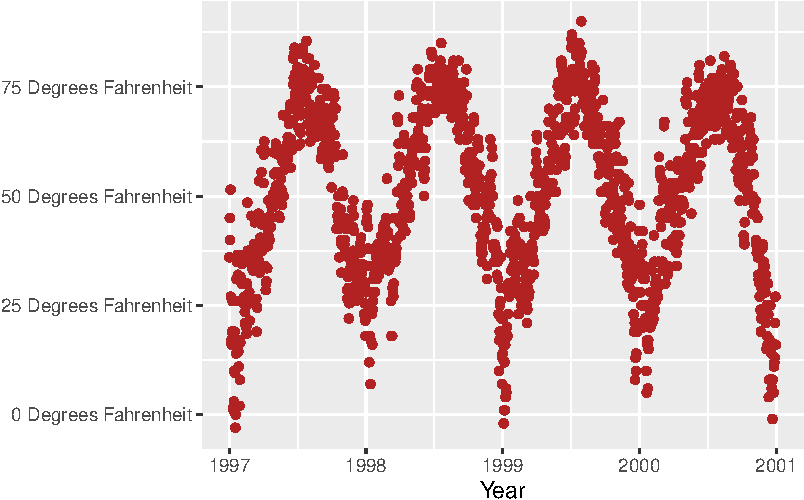
\includegraphics{ch4_files/figure-pdf/labs-alt-1.pdf}

\bookmarksetup{startatroot}

\chapter{Working with Titles}\label{titles}

\section{Add a Title}\label{add-a-title}

We can add a title by using the \texttt{ggtitle()} function:

\begin{Shaded}
\begin{Highlighting}[]
\FunctionTok{ggplot}\NormalTok{(chic, }\FunctionTok{aes}\NormalTok{(}\AttributeTok{x =}\NormalTok{ date, }\AttributeTok{y =}\NormalTok{ temp)) }\SpecialCharTok{+}
  \FunctionTok{geom\_point}\NormalTok{(}\AttributeTok{color =} \StringTok{"firebrick"}\NormalTok{) }\SpecialCharTok{+}
  \FunctionTok{labs}\NormalTok{(}\AttributeTok{x =} \StringTok{"Year"}\NormalTok{, }\AttributeTok{y =} \StringTok{"Temperature (°F)"}\NormalTok{) }\SpecialCharTok{+}
  \FunctionTok{ggtitle}\NormalTok{(}\StringTok{"Temperatures in Chicago"}\NormalTok{)}
\end{Highlighting}
\end{Shaded}

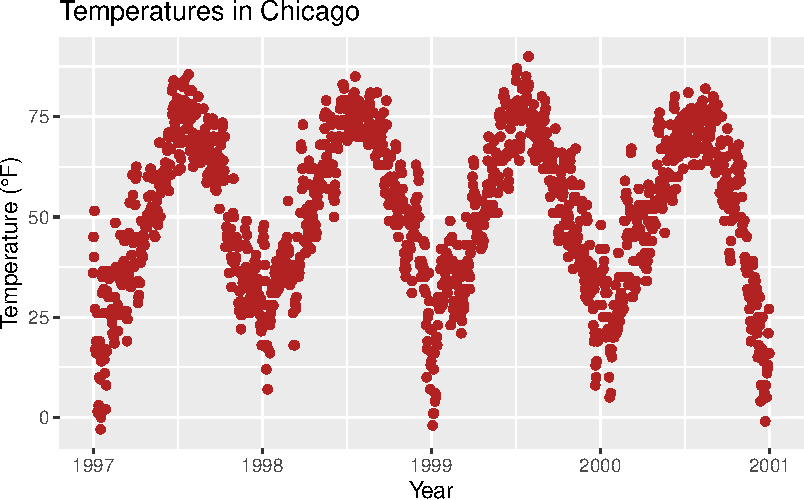
\includegraphics{ch5_files/figure-pdf/title-1.pdf}

Alternatively, you can utilize \texttt{labs()}. Here, you can include
multiple arguments, such as a subtitle, a caption, and a tag, in
addition to axis titles as demonstrated earlier:

\begin{Shaded}
\begin{Highlighting}[]
\FunctionTok{ggplot}\NormalTok{(chic, }\FunctionTok{aes}\NormalTok{(}\AttributeTok{x =}\NormalTok{ date, }\AttributeTok{y =}\NormalTok{ temp)) }\SpecialCharTok{+}
  \FunctionTok{geom\_point}\NormalTok{(}\AttributeTok{color =} \StringTok{"firebrick"}\NormalTok{) }\SpecialCharTok{+}
  \FunctionTok{labs}\NormalTok{(}\AttributeTok{x =} \StringTok{"Year"}\NormalTok{, }\AttributeTok{y =} \StringTok{"Temperature (°F)"}\NormalTok{,}
       \AttributeTok{title =} \StringTok{"Temperatures in Chicago"}\NormalTok{,}
       \AttributeTok{subtitle =} \StringTok{"Seasonal pattern of daily temperatures from 1997 to 2001"}\NormalTok{,}
       \AttributeTok{caption =} \StringTok{"Data: NMMAPS"}\NormalTok{,}
       \AttributeTok{tag =} \StringTok{"Fig. 1"}\NormalTok{)}
\end{Highlighting}
\end{Shaded}

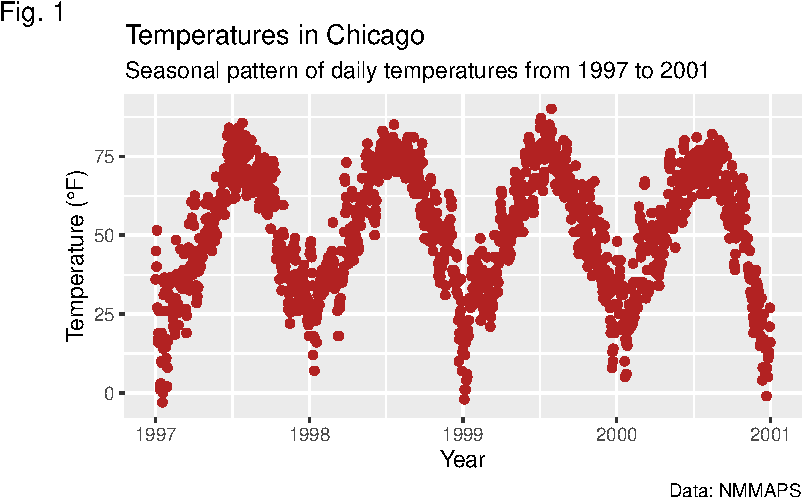
\includegraphics{ch5_files/figure-pdf/title-labs-1.pdf}

\section{Making Title Bold \& Adding a Space at the
Baseline}\label{making-title-bold-adding-a-space-at-the-baseline}

Once again, to adjust the properties of a theme element, we employ the
\texttt{theme()} function. Similar to modifying text elements like
\texttt{axis.title} and \texttt{axis.text}, we can alter the font face
and margin for the title. These modifications apply not only to the
title but also to other labels such as \texttt{plot.subtitle},
\texttt{plot.caption}, \texttt{plot.tag}, \texttt{legend.title},
\texttt{legend.text}, \texttt{axis.title}, and \texttt{axis.text}.

\begin{Shaded}
\begin{Highlighting}[]
\FunctionTok{ggplot}\NormalTok{(chic, }\FunctionTok{aes}\NormalTok{(}\AttributeTok{x =}\NormalTok{ date, }\AttributeTok{y =}\NormalTok{ temp)) }\SpecialCharTok{+}
  \FunctionTok{geom\_point}\NormalTok{(}\AttributeTok{color =} \StringTok{"firebrick"}\NormalTok{) }\SpecialCharTok{+}
  \FunctionTok{labs}\NormalTok{(}\AttributeTok{x =} \StringTok{"Year"}\NormalTok{, }\AttributeTok{y =} \StringTok{"Temperature (°F)"}\NormalTok{,}
       \AttributeTok{title =} \StringTok{"Temperatures in Chicago"}\NormalTok{) }\SpecialCharTok{+}
  \FunctionTok{theme}\NormalTok{(}\AttributeTok{plot.title =} \FunctionTok{element\_text}\NormalTok{(}\AttributeTok{face =} \StringTok{"bold"}\NormalTok{,}
                                  \AttributeTok{margin =} \FunctionTok{margin}\NormalTok{(}\DecValTok{10}\NormalTok{, }\DecValTok{0}\NormalTok{, }\DecValTok{10}\NormalTok{, }\DecValTok{0}\NormalTok{),}
                                  \AttributeTok{size =} \DecValTok{14}\NormalTok{))}
\end{Highlighting}
\end{Shaded}

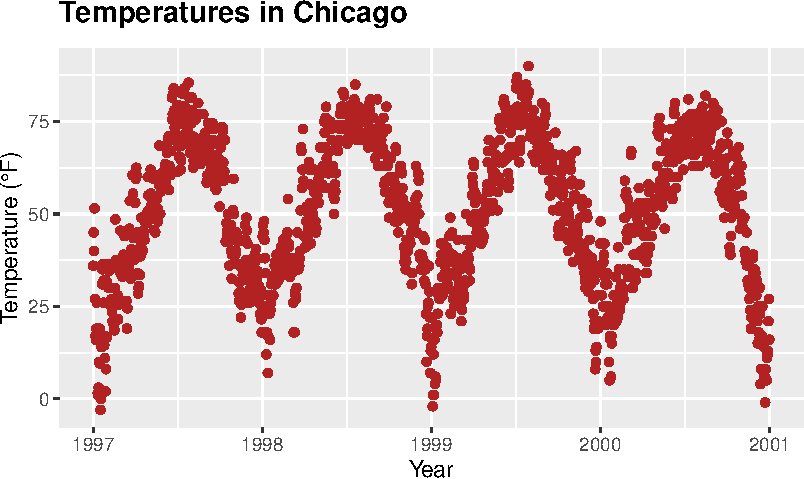
\includegraphics{ch5_files/figure-pdf/title-bold-1.pdf}

💡 \textbf{A helpful mnemonic for remembering the order of the margin
arguments is ``\emph{t}-\emph{r}-oub-\emph{l}-\emph{e}'', which
corresponds to the first letter of each side.}

\section{Adjusting Position of
Titles}\label{adjusting-position-of-titles}

The general alignment (left, center, right) is controlled by
\texttt{hjust} (horizontal adjustment):

\begin{Shaded}
\begin{Highlighting}[]
\FunctionTok{ggplot}\NormalTok{(chic, }\FunctionTok{aes}\NormalTok{(}\AttributeTok{x =}\NormalTok{ date, }\AttributeTok{y =}\NormalTok{ temp)) }\SpecialCharTok{+}
  \FunctionTok{geom\_point}\NormalTok{(}\AttributeTok{color =} \StringTok{"firebrick"}\NormalTok{) }\SpecialCharTok{+}
  \FunctionTok{labs}\NormalTok{(}\AttributeTok{x =} \StringTok{"Year"}\NormalTok{, }\AttributeTok{y =} \ConstantTok{NULL}\NormalTok{,}
       \AttributeTok{title =} \StringTok{"Temperatures in Chicago"}\NormalTok{,}
       \AttributeTok{caption =} \StringTok{"Data: NMMAPS"}\NormalTok{) }\SpecialCharTok{+}
  \FunctionTok{theme}\NormalTok{(}\AttributeTok{plot.title =} \FunctionTok{element\_text}\NormalTok{(}\AttributeTok{hjust =} \DecValTok{1}\NormalTok{, }\AttributeTok{size =} \DecValTok{16}\NormalTok{, }\AttributeTok{face =} \StringTok{"bold.italic"}\NormalTok{))}
\end{Highlighting}
\end{Shaded}

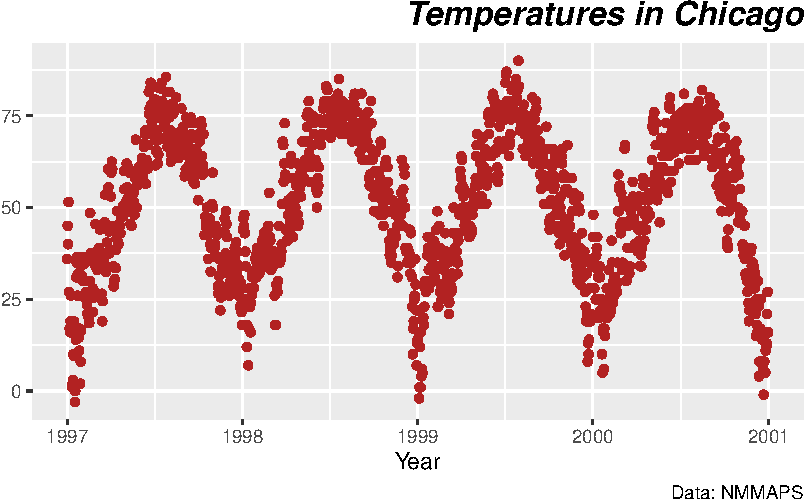
\includegraphics{ch5_files/figure-pdf/title-adjust-1.pdf}

Certainly, it's also possible to adjust the vertical alignment, which is
controlled by \texttt{vjust}. Since 2019, users have been able to
specify the alignment of the title, subtitle, and caption either based
on the panel area (the default) or the plot margin via
\texttt{plot.title.position} and \texttt{plot.caption.position}. The
latter is often the preferred choice from a design perspective, as it
yields better results in most cases. Many users have expressed
satisfaction with this new feature, particularly as it addresses issues
with alignment, especially when dealing with very long y-axis labels:

\begin{Shaded}
\begin{Highlighting}[]
\NormalTok{(g }\OtherTok{\textless{}{-}} \FunctionTok{ggplot}\NormalTok{(chic, }\FunctionTok{aes}\NormalTok{(}\AttributeTok{x =}\NormalTok{ date, }\AttributeTok{y =}\NormalTok{ temp)) }\SpecialCharTok{+}
  \FunctionTok{geom\_point}\NormalTok{(}\AttributeTok{color =} \StringTok{"firebrick"}\NormalTok{) }\SpecialCharTok{+}
  \FunctionTok{scale\_y\_continuous}\NormalTok{(}\AttributeTok{label =} \ControlFlowTok{function}\NormalTok{(x) \{}\FunctionTok{return}\NormalTok{(}\FunctionTok{paste}\NormalTok{(x, }\StringTok{"Degrees Fahrenheit"}\NormalTok{))\}) }\SpecialCharTok{+}
  \FunctionTok{labs}\NormalTok{(}\AttributeTok{x =} \StringTok{"Year"}\NormalTok{, }\AttributeTok{y =} \ConstantTok{NULL}\NormalTok{,}
       \AttributeTok{title =} \StringTok{"Temperatures in Chicago between 1997 and 2001 in Degrees Fahrenheit"}\NormalTok{,}
       \AttributeTok{caption =} \StringTok{"Data: NMMAPS"}\NormalTok{) }\SpecialCharTok{+}
  \FunctionTok{theme}\NormalTok{(}\AttributeTok{plot.title =} \FunctionTok{element\_text}\NormalTok{(}\AttributeTok{size =} \DecValTok{14}\NormalTok{, }\AttributeTok{face =} \StringTok{"bold.italic"}\NormalTok{),}
        \AttributeTok{plot.caption =} \FunctionTok{element\_text}\NormalTok{(}\AttributeTok{hjust =} \DecValTok{0}\NormalTok{)))}
\end{Highlighting}
\end{Shaded}

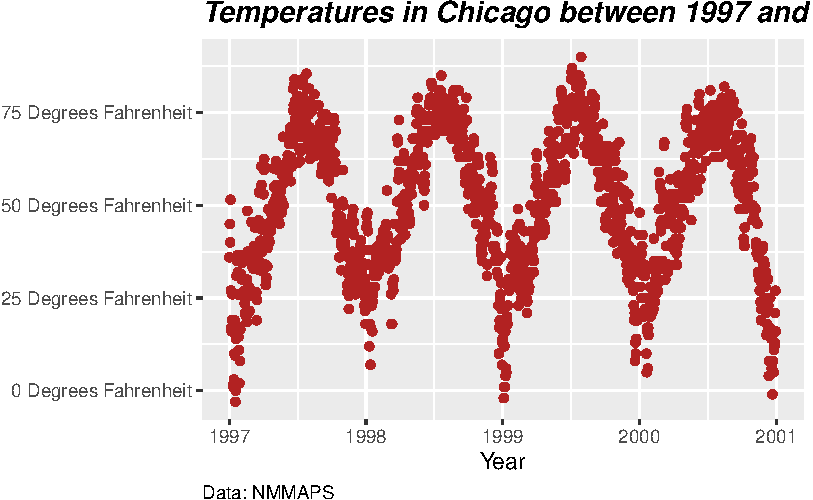
\includegraphics{ch5_files/figure-pdf/title-position-default-1.pdf}

\begin{Shaded}
\begin{Highlighting}[]
\NormalTok{g }\SpecialCharTok{+} \FunctionTok{theme}\NormalTok{(}\AttributeTok{plot.title.position =} \StringTok{"plot"}\NormalTok{,}
          \AttributeTok{plot.caption.position =} \StringTok{"plot"}\NormalTok{)}
\end{Highlighting}
\end{Shaded}

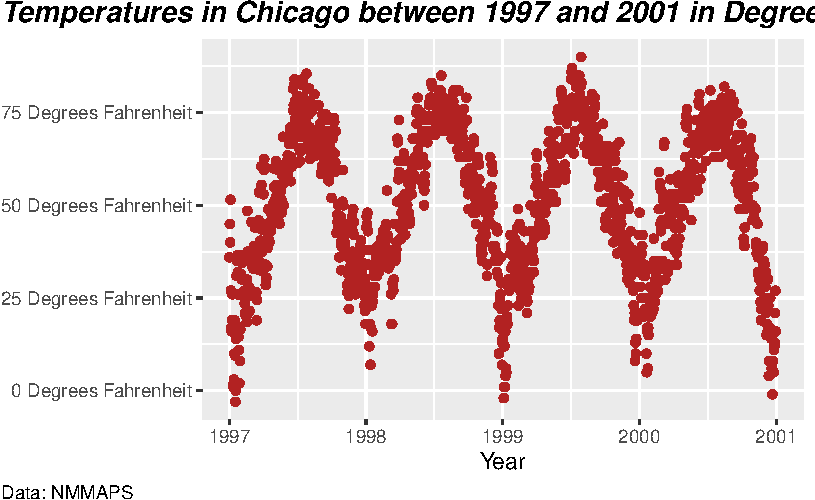
\includegraphics{ch5_files/figure-pdf/title-position-plot-1.pdf}

\section{Using a Non-Traditional Font in Your
Title}\label{using-a-non-traditional-font-in-your-title}

You can incorporate different fonts, not just the default one provided
by ggplot (which can vary between operating systems). Several packages
facilitate the usage of fonts installed on your machine, such as the
\href{https://github.com/yixuan/showtext}{\texttt{showtext} package},
which simplifies the utilization of various font types (TrueType,
OpenType, Type 1, web fonts, etc.) in R plots.

Once the package is loaded, you'll need to import the desired font,
which must also be installed on your device. I often utilize
\href{https://fonts.google.com/}{Google fonts}, which can be imported
using the \texttt{font\_add\_google()} function. However, you can add
other fonts using \texttt{font\_add()} as well. It's important to note
that even when using Google fonts, you must install the font and restart
RStudio to apply it. if you found any warnings after doing all the
steps, or the fonts aren't working. Just install \texttt{extrafont}
package and run \texttt{font\_import()} function to import all the fonts
in your system. and then
\texttt{loadfonts(device\ =\ "win",\ quiet\ =\ TRUE)} to load the fonts.
It'll work like a charm. You can also check the available fonts in your
system by running \texttt{fonts()}.

\begin{Shaded}
\begin{Highlighting}[]
\FunctionTok{library}\NormalTok{(showtext)}
\FunctionTok{library}\NormalTok{(extrafont)}
\FunctionTok{font\_add\_google}\NormalTok{(}\StringTok{"Playfair Display"}\NormalTok{, }\DocumentationTok{\#\# name of Google font}
                \StringTok{"Playfair Display"}\NormalTok{)  }\DocumentationTok{\#\# name that will be used in R}
\FunctionTok{font\_add\_google}\NormalTok{(}\StringTok{"Bangers"}\NormalTok{, }\StringTok{"Bangers"}\NormalTok{)}
\FunctionTok{loadfonts}\NormalTok{(}\AttributeTok{device =} \StringTok{"win"}\NormalTok{, }\AttributeTok{quiet =} \ConstantTok{TRUE}\NormalTok{)}
\end{Highlighting}
\end{Shaded}

Now, we can use those font families by \texttt{theme()} function:

\begin{Shaded}
\begin{Highlighting}[]
\FunctionTok{ggplot}\NormalTok{(chic, }\FunctionTok{aes}\NormalTok{(}\AttributeTok{x =}\NormalTok{ date, }\AttributeTok{y =}\NormalTok{ temp)) }\SpecialCharTok{+}
  \FunctionTok{geom\_point}\NormalTok{(}\AttributeTok{color =} \StringTok{"firebrick"}\NormalTok{) }\SpecialCharTok{+}
  \FunctionTok{labs}\NormalTok{(}\AttributeTok{x =} \StringTok{"Year"}\NormalTok{, }\AttributeTok{y =} \StringTok{"Temperature (°F)"}\NormalTok{,}
       \AttributeTok{title =} \StringTok{"Temperatures in Chicago"}\NormalTok{,}
       \AttributeTok{subtitle =} \StringTok{"Daily temperatures in °F from 1997 to 2001"}\NormalTok{) }\SpecialCharTok{+}
  \FunctionTok{theme}\NormalTok{(}\AttributeTok{plot.title =} \FunctionTok{element\_text}\NormalTok{(}\AttributeTok{family =} \StringTok{"Bangers"}\NormalTok{, }\AttributeTok{hjust =}\NormalTok{ .}\DecValTok{5}\NormalTok{, }\AttributeTok{size =} \DecValTok{25}\NormalTok{),}
        \AttributeTok{plot.subtitle =} \FunctionTok{element\_text}\NormalTok{(}\AttributeTok{family =} \StringTok{"Playfair Display"}\NormalTok{, }\AttributeTok{hjust =}\NormalTok{ .}\DecValTok{5}\NormalTok{, }\AttributeTok{size =} \DecValTok{15}\NormalTok{))}
\end{Highlighting}
\end{Shaded}

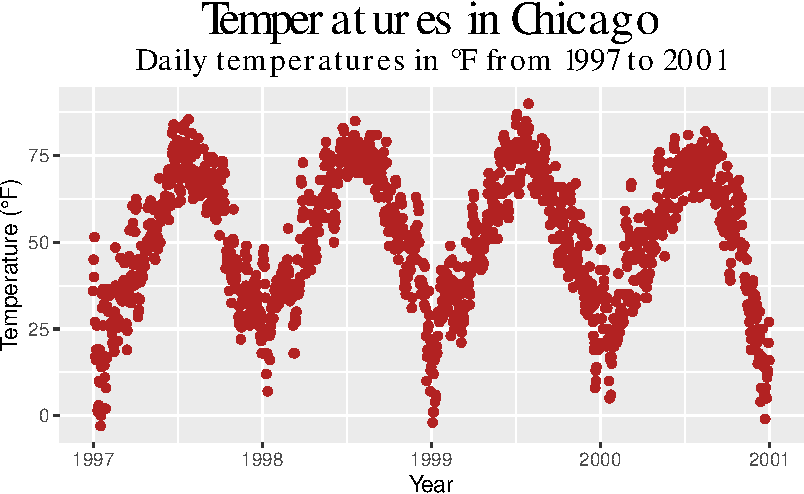
\includegraphics{ch5_files/figure-pdf/title-style-1.pdf}

You can also establish a non-default font for all text elements of your
plots. For more details, refer to the section
\hyperref[themes]{``Working with Themes''}. In this case, I'll use
\emph{Roboto Condensed} as the new font for all subsequent plots.

\begin{Shaded}
\begin{Highlighting}[]
\FunctionTok{font\_add\_google}\NormalTok{(}\StringTok{"Roboto Condensed"}\NormalTok{, }\StringTok{"Roboto Condensed"}\NormalTok{)}
\FunctionTok{theme\_set}\NormalTok{(}\FunctionTok{theme\_bw}\NormalTok{(}\AttributeTok{base\_size =} \DecValTok{12}\NormalTok{, }\AttributeTok{base\_family =} \StringTok{"Roboto Condensed"}\NormalTok{))}
\end{Highlighting}
\end{Shaded}

(Previously, this tutorial utilized the
\href{https://cran.r-project.org/web/packages/extrafont/README.html}{\texttt{\{extrafont\}}
package}, which performed admirably until last year. However, suddenly I
encountered issues where I couldn't add any new fonts, and even after
acquiring a new laptop, the package failed to detect any fonts
altogether. As an alternative, I typically recommend the
\href{https://ragg.r-lib.org/}{\texttt{\{ragg\}} package} now. However,
I encountered difficulties in making it work for my homepage. Therefore,
I'm utilizing the \texttt{\{showtext\}} package, which is also
excellent, albeit with a key distinction: you need to explicitly import
the font you wish to use with \texttt{\{showtext\}}. Nonetheless, it
appears that there are some technical challenges that are not optimally
resolved by \texttt{\{showtext\}} (as mentioned in
\href{https://twitter.com/thomasp85/status/1355083725156077571}{this
Twitter thread}), so you may want to consider using the package only as
a last resort.)

\section{Adjusting Spacing in Multi-Line
Text}\label{adjusting-spacing-in-multi-line-text}

To modify the spacing between lines, you can utilize the
\texttt{lineheight} argument. In the following example, I've compressed
the lines together (lineheight \textless{} 1).

\begin{Shaded}
\begin{Highlighting}[]
\FunctionTok{ggplot}\NormalTok{(chic, }\FunctionTok{aes}\NormalTok{(}\AttributeTok{x =}\NormalTok{ date, }\AttributeTok{y =}\NormalTok{ temp)) }\SpecialCharTok{+}
  \FunctionTok{geom\_point}\NormalTok{(}\AttributeTok{color =} \StringTok{"firebrick"}\NormalTok{) }\SpecialCharTok{+}
  \FunctionTok{labs}\NormalTok{(}\AttributeTok{x =} \StringTok{"Year"}\NormalTok{, }\AttributeTok{y =} \StringTok{"Temperature (°F)"}\NormalTok{) }\SpecialCharTok{+}
  \FunctionTok{ggtitle}\NormalTok{(}\StringTok{"Temperatures in Chicago}\SpecialCharTok{\textbackslash{}n}\StringTok{from 1997 to 2001"}\NormalTok{) }\SpecialCharTok{+}
  \FunctionTok{theme}\NormalTok{(}\AttributeTok{plot.title =} \FunctionTok{element\_text}\NormalTok{(}\AttributeTok{lineheight =}\NormalTok{ .}\DecValTok{8}\NormalTok{, }\AttributeTok{size =} \DecValTok{16}\NormalTok{))}
\end{Highlighting}
\end{Shaded}

\begin{verbatim}
Warning in grid.Call(C_stringMetric, as.graphicsAnnot(x$label)): font metrics
unknown for character 0x4d
\end{verbatim}

\begin{verbatim}
Warning in grid.Call(C_stringMetric, as.graphicsAnnot(x$label)): font width
unknown for character 0x67
\end{verbatim}

\begin{verbatim}
Warning in grid.Call(C_stringMetric, as.graphicsAnnot(x$label)): font width
unknown for character 0x6a
\end{verbatim}

\begin{verbatim}
Warning in grid.Call(C_stringMetric, as.graphicsAnnot(x$label)): font width
unknown for character 0x70
\end{verbatim}

\begin{verbatim}
Warning in grid.Call(C_stringMetric, as.graphicsAnnot(x$label)): font width
unknown for character 0x71
\end{verbatim}

\begin{verbatim}
Warning in grid.Call(C_stringMetric, as.graphicsAnnot(x$label)): font width
unknown for character 0x79
\end{verbatim}

\begin{verbatim}
Warning in grid.Call(C_stringMetric, as.graphicsAnnot(x$label)): font width
unknown for character 0x51
\end{verbatim}

\begin{verbatim}
Warning in grid.Call(C_textBounds, as.graphicsAnnot(x$label), x$x, x$y, : font
width unknown for character 0x31
\end{verbatim}

\begin{verbatim}
Warning in grid.Call(C_textBounds, as.graphicsAnnot(x$label), x$x, x$y, : font
width unknown for character 0x39

Warning in grid.Call(C_textBounds, as.graphicsAnnot(x$label), x$x, x$y, : font
width unknown for character 0x39
\end{verbatim}

\begin{verbatim}
Warning in grid.Call(C_textBounds, as.graphicsAnnot(x$label), x$x, x$y, : font
width unknown for character 0x37
\end{verbatim}

\begin{verbatim}
Warning in grid.Call(C_textBounds, as.graphicsAnnot(x$label), x$x, x$y, : font
width unknown for character 0x31
\end{verbatim}

\begin{verbatim}
Warning in grid.Call(C_textBounds, as.graphicsAnnot(x$label), x$x, x$y, : font
width unknown for character 0x39

Warning in grid.Call(C_textBounds, as.graphicsAnnot(x$label), x$x, x$y, : font
width unknown for character 0x39
\end{verbatim}

\begin{verbatim}
Warning in grid.Call(C_textBounds, as.graphicsAnnot(x$label), x$x, x$y, : font
width unknown for character 0x38
\end{verbatim}

\begin{verbatim}
Warning in grid.Call(C_textBounds, as.graphicsAnnot(x$label), x$x, x$y, : font
width unknown for character 0x31
\end{verbatim}

\begin{verbatim}
Warning in grid.Call(C_textBounds, as.graphicsAnnot(x$label), x$x, x$y, : font
width unknown for character 0x39

Warning in grid.Call(C_textBounds, as.graphicsAnnot(x$label), x$x, x$y, : font
width unknown for character 0x39

Warning in grid.Call(C_textBounds, as.graphicsAnnot(x$label), x$x, x$y, : font
width unknown for character 0x39
\end{verbatim}

\begin{verbatim}
Warning in grid.Call(C_textBounds, as.graphicsAnnot(x$label), x$x, x$y, : font
width unknown for character 0x32
\end{verbatim}

\begin{verbatim}
Warning in grid.Call(C_textBounds, as.graphicsAnnot(x$label), x$x, x$y, : font
width unknown for character 0x30

Warning in grid.Call(C_textBounds, as.graphicsAnnot(x$label), x$x, x$y, : font
width unknown for character 0x30

Warning in grid.Call(C_textBounds, as.graphicsAnnot(x$label), x$x, x$y, : font
width unknown for character 0x30
\end{verbatim}

\begin{verbatim}
Warning in grid.Call(C_textBounds, as.graphicsAnnot(x$label), x$x, x$y, : font
width unknown for character 0x32
\end{verbatim}

\begin{verbatim}
Warning in grid.Call(C_textBounds, as.graphicsAnnot(x$label), x$x, x$y, : font
width unknown for character 0x30

Warning in grid.Call(C_textBounds, as.graphicsAnnot(x$label), x$x, x$y, : font
width unknown for character 0x30
\end{verbatim}

\begin{verbatim}
Warning in grid.Call(C_textBounds, as.graphicsAnnot(x$label), x$x, x$y, : font
width unknown for character 0x31
\end{verbatim}

\begin{verbatim}
Warning in grid.Call(C_textBounds, as.graphicsAnnot(x$label), x$x, x$y, : font
width unknown for character 0x30
\end{verbatim}

\begin{verbatim}
Warning in grid.Call(C_textBounds, as.graphicsAnnot(x$label), x$x, x$y, : font
width unknown for character 0x32
\end{verbatim}

\begin{verbatim}
Warning in grid.Call(C_textBounds, as.graphicsAnnot(x$label), x$x, x$y, : font
width unknown for character 0x35

Warning in grid.Call(C_textBounds, as.graphicsAnnot(x$label), x$x, x$y, : font
width unknown for character 0x35
\end{verbatim}

\begin{verbatim}
Warning in grid.Call(C_textBounds, as.graphicsAnnot(x$label), x$x, x$y, : font
width unknown for character 0x30
\end{verbatim}

\begin{verbatim}
Warning in grid.Call(C_textBounds, as.graphicsAnnot(x$label), x$x, x$y, : font
width unknown for character 0x37
\end{verbatim}

\begin{verbatim}
Warning in grid.Call(C_textBounds, as.graphicsAnnot(x$label), x$x, x$y, : font
width unknown for character 0x35
\end{verbatim}

\begin{verbatim}
Warning in grid.Call(C_stringMetric, as.graphicsAnnot(x$label)): font metrics
unknown for character 0x4d
\end{verbatim}

\begin{verbatim}
Warning in grid.Call(C_stringMetric, as.graphicsAnnot(x$label)): font width
unknown for character 0x67
\end{verbatim}

\begin{verbatim}
Warning in grid.Call(C_stringMetric, as.graphicsAnnot(x$label)): font width
unknown for character 0x6a
\end{verbatim}

\begin{verbatim}
Warning in grid.Call(C_stringMetric, as.graphicsAnnot(x$label)): font width
unknown for character 0x70
\end{verbatim}

\begin{verbatim}
Warning in grid.Call(C_stringMetric, as.graphicsAnnot(x$label)): font width
unknown for character 0x71
\end{verbatim}

\begin{verbatim}
Warning in grid.Call(C_stringMetric, as.graphicsAnnot(x$label)): font width
unknown for character 0x79
\end{verbatim}

\begin{verbatim}
Warning in grid.Call(C_stringMetric, as.graphicsAnnot(x$label)): font width
unknown for character 0x51
\end{verbatim}

\begin{verbatim}
Warning in grid.Call(C_stringMetric, as.graphicsAnnot(x$label)): font metrics
unknown for character 0x4d
\end{verbatim}

\begin{verbatim}
Warning in grid.Call(C_stringMetric, as.graphicsAnnot(x$label)): font width
unknown for character 0x67
\end{verbatim}

\begin{verbatim}
Warning in grid.Call(C_stringMetric, as.graphicsAnnot(x$label)): font width
unknown for character 0x6a
\end{verbatim}

\begin{verbatim}
Warning in grid.Call(C_stringMetric, as.graphicsAnnot(x$label)): font width
unknown for character 0x70
\end{verbatim}

\begin{verbatim}
Warning in grid.Call(C_stringMetric, as.graphicsAnnot(x$label)): font width
unknown for character 0x71
\end{verbatim}

\begin{verbatim}
Warning in grid.Call(C_stringMetric, as.graphicsAnnot(x$label)): font width
unknown for character 0x79
\end{verbatim}

\begin{verbatim}
Warning in grid.Call(C_stringMetric, as.graphicsAnnot(x$label)): font width
unknown for character 0x51
\end{verbatim}

\begin{verbatim}
Warning in grid.Call(C_textBounds, as.graphicsAnnot(x$label), x$x, x$y, : font
width unknown for character 0x54
\end{verbatim}

\begin{verbatim}
Warning in grid.Call(C_textBounds, as.graphicsAnnot(x$label), x$x, x$y, : font
width unknown for character 0xab
\end{verbatim}

\begin{verbatim}
Warning in grid.Call(C_textBounds, as.graphicsAnnot(x$label), x$x, x$y, : font
width unknown for character 0xcd
\end{verbatim}

\begin{verbatim}
Warning in grid.Call(C_textBounds, as.graphicsAnnot(x$label), x$x, x$y, : font
width unknown for character 0xf4
\end{verbatim}

\begin{verbatim}
Warning in grid.Call(C_textBounds, as.graphicsAnnot(x$label), x$x, x$y, : font
width unknown for character 0xfd
\end{verbatim}

\begin{verbatim}
Warning in grid.Call(C_textBounds, as.graphicsAnnot(x$label), x$x, x$y, : font
width unknown for character 0x7f
\end{verbatim}

\begin{verbatim}
Warning in grid.Call(C_textBounds, as.graphicsAnnot(x$label), x$x, x$y, : font
metrics unknown for character 0x4d
\end{verbatim}

\begin{verbatim}
Warning in grid.Call(C_textBounds, as.graphicsAnnot(x$label), x$x, x$y, : font
width unknown for character 0x54
\end{verbatim}

\begin{verbatim}
Warning in grid.Call(C_textBounds, as.graphicsAnnot(x$label), x$x, x$y, : font
width unknown for character 0x65
\end{verbatim}

\begin{verbatim}
Warning in grid.Call(C_textBounds, as.graphicsAnnot(x$label), x$x, x$y, : font
width unknown for character 0x6d
\end{verbatim}

\begin{verbatim}
Warning in grid.Call(C_textBounds, as.graphicsAnnot(x$label), x$x, x$y, : font
width unknown for character 0x70
\end{verbatim}

\begin{verbatim}
Warning in grid.Call(C_textBounds, as.graphicsAnnot(x$label), x$x, x$y, : font
width unknown for character 0x65
\end{verbatim}

\begin{verbatim}
Warning in grid.Call(C_textBounds, as.graphicsAnnot(x$label), x$x, x$y, : font
width unknown for character 0x72
\end{verbatim}

\begin{verbatim}
Warning in grid.Call(C_textBounds, as.graphicsAnnot(x$label), x$x, x$y, : font
width unknown for character 0x61
\end{verbatim}

\begin{verbatim}
Warning in grid.Call(C_textBounds, as.graphicsAnnot(x$label), x$x, x$y, : font
width unknown for character 0x74
\end{verbatim}

\begin{verbatim}
Warning in grid.Call(C_textBounds, as.graphicsAnnot(x$label), x$x, x$y, : font
width unknown for character 0x75
\end{verbatim}

\begin{verbatim}
Warning in grid.Call(C_textBounds, as.graphicsAnnot(x$label), x$x, x$y, : font
width unknown for character 0x72
\end{verbatim}

\begin{verbatim}
Warning in grid.Call(C_textBounds, as.graphicsAnnot(x$label), x$x, x$y, : font
width unknown for character 0x65
\end{verbatim}

\begin{verbatim}
Warning in grid.Call(C_textBounds, as.graphicsAnnot(x$label), x$x, x$y, : font
width unknown for character 0x73
\end{verbatim}

\begin{verbatim}
Warning in grid.Call(C_textBounds, as.graphicsAnnot(x$label), x$x, x$y, : font
width unknown for character 0x20
\end{verbatim}

\begin{verbatim}
Warning in grid.Call(C_textBounds, as.graphicsAnnot(x$label), x$x, x$y, : font
width unknown for character 0x69
\end{verbatim}

\begin{verbatim}
Warning in grid.Call(C_textBounds, as.graphicsAnnot(x$label), x$x, x$y, : font
width unknown for character 0x6e
\end{verbatim}

\begin{verbatim}
Warning in grid.Call(C_textBounds, as.graphicsAnnot(x$label), x$x, x$y, : font
width unknown for character 0x20
\end{verbatim}

\begin{verbatim}
Warning in grid.Call(C_textBounds, as.graphicsAnnot(x$label), x$x, x$y, : font
width unknown for character 0x43
\end{verbatim}

\begin{verbatim}
Warning in grid.Call(C_textBounds, as.graphicsAnnot(x$label), x$x, x$y, : font
width unknown for character 0x68
\end{verbatim}

\begin{verbatim}
Warning in grid.Call(C_textBounds, as.graphicsAnnot(x$label), x$x, x$y, : font
width unknown for character 0x69
\end{verbatim}

\begin{verbatim}
Warning in grid.Call(C_textBounds, as.graphicsAnnot(x$label), x$x, x$y, : font
width unknown for character 0x63
\end{verbatim}

\begin{verbatim}
Warning in grid.Call(C_textBounds, as.graphicsAnnot(x$label), x$x, x$y, : font
width unknown for character 0x61
\end{verbatim}

\begin{verbatim}
Warning in grid.Call(C_textBounds, as.graphicsAnnot(x$label), x$x, x$y, : font
width unknown for character 0x67
\end{verbatim}

\begin{verbatim}
Warning in grid.Call(C_textBounds, as.graphicsAnnot(x$label), x$x, x$y, : font
width unknown for character 0x6f
\end{verbatim}

\begin{verbatim}
Warning in grid.Call(C_textBounds, as.graphicsAnnot(x$label), x$x, x$y, : font
width unknown for character 0x66
\end{verbatim}

\begin{verbatim}
Warning in grid.Call(C_textBounds, as.graphicsAnnot(x$label), x$x, x$y, : font
width unknown for character 0x72
\end{verbatim}

\begin{verbatim}
Warning in grid.Call(C_textBounds, as.graphicsAnnot(x$label), x$x, x$y, : font
width unknown for character 0x6f
\end{verbatim}

\begin{verbatim}
Warning in grid.Call(C_textBounds, as.graphicsAnnot(x$label), x$x, x$y, : font
width unknown for character 0x6d
\end{verbatim}

\begin{verbatim}
Warning in grid.Call(C_textBounds, as.graphicsAnnot(x$label), x$x, x$y, : font
width unknown for character 0x20
\end{verbatim}

\begin{verbatim}
Warning in grid.Call(C_textBounds, as.graphicsAnnot(x$label), x$x, x$y, : font
width unknown for character 0x31
\end{verbatim}

\begin{verbatim}
Warning in grid.Call(C_textBounds, as.graphicsAnnot(x$label), x$x, x$y, : font
width unknown for character 0x39

Warning in grid.Call(C_textBounds, as.graphicsAnnot(x$label), x$x, x$y, : font
width unknown for character 0x39
\end{verbatim}

\begin{verbatim}
Warning in grid.Call(C_textBounds, as.graphicsAnnot(x$label), x$x, x$y, : font
width unknown for character 0x37
\end{verbatim}

\begin{verbatim}
Warning in grid.Call(C_textBounds, as.graphicsAnnot(x$label), x$x, x$y, : font
width unknown for character 0x20
\end{verbatim}

\begin{verbatim}
Warning in grid.Call(C_textBounds, as.graphicsAnnot(x$label), x$x, x$y, : font
width unknown for character 0x74
\end{verbatim}

\begin{verbatim}
Warning in grid.Call(C_textBounds, as.graphicsAnnot(x$label), x$x, x$y, : font
width unknown for character 0x6f
\end{verbatim}

\begin{verbatim}
Warning in grid.Call(C_textBounds, as.graphicsAnnot(x$label), x$x, x$y, : font
width unknown for character 0x20
\end{verbatim}

\begin{verbatim}
Warning in grid.Call(C_textBounds, as.graphicsAnnot(x$label), x$x, x$y, : font
width unknown for character 0x32
\end{verbatim}

\begin{verbatim}
Warning in grid.Call(C_textBounds, as.graphicsAnnot(x$label), x$x, x$y, : font
width unknown for character 0x30

Warning in grid.Call(C_textBounds, as.graphicsAnnot(x$label), x$x, x$y, : font
width unknown for character 0x30
\end{verbatim}

\begin{verbatim}
Warning in grid.Call(C_textBounds, as.graphicsAnnot(x$label), x$x, x$y, : font
width unknown for character 0x31
\end{verbatim}

\begin{verbatim}
Warning in grid.Call(C_textBounds, as.graphicsAnnot(x$label), x$x, x$y, : font
metrics unknown for character 0x4d
\end{verbatim}

\begin{verbatim}
Warning in grid.Call(C_textBounds, as.graphicsAnnot(x$label), x$x, x$y, : font
width unknown for character 0x59
\end{verbatim}

\begin{verbatim}
Warning in grid.Call(C_textBounds, as.graphicsAnnot(x$label), x$x, x$y, : font
width unknown for character 0x65
\end{verbatim}

\begin{verbatim}
Warning in grid.Call(C_textBounds, as.graphicsAnnot(x$label), x$x, x$y, : font
width unknown for character 0x61
\end{verbatim}

\begin{verbatim}
Warning in grid.Call(C_textBounds, as.graphicsAnnot(x$label), x$x, x$y, : font
width unknown for character 0x72
\end{verbatim}

\begin{verbatim}
Warning in grid.Call(C_textBounds, as.graphicsAnnot(x$label), x$x, x$y, : font
metrics unknown for character 0x4d
\end{verbatim}

\begin{verbatim}
Warning in grid.Call.graphics(C_text, as.graphicsAnnot(x$label), x$x, x$y, :
font width unknown for character 0x30
\end{verbatim}

\begin{verbatim}
Warning in grid.Call.graphics(C_text, as.graphicsAnnot(x$label), x$x, x$y, :
font metrics unknown for character 0x4d
\end{verbatim}

\begin{verbatim}
Warning in grid.Call.graphics(C_text, as.graphicsAnnot(x$label), x$x, x$y, :
font width unknown for character 0x32
\end{verbatim}

\begin{verbatim}
Warning in grid.Call.graphics(C_text, as.graphicsAnnot(x$label), x$x, x$y, :
font width unknown for character 0x35

Warning in grid.Call.graphics(C_text, as.graphicsAnnot(x$label), x$x, x$y, :
font width unknown for character 0x35
\end{verbatim}

\begin{verbatim}
Warning in grid.Call.graphics(C_text, as.graphicsAnnot(x$label), x$x, x$y, :
font width unknown for character 0x30
\end{verbatim}

\begin{verbatim}
Warning in grid.Call.graphics(C_text, as.graphicsAnnot(x$label), x$x, x$y, :
font width unknown for character 0x37
\end{verbatim}

\begin{verbatim}
Warning in grid.Call.graphics(C_text, as.graphicsAnnot(x$label), x$x, x$y, :
font width unknown for character 0x35
\end{verbatim}

\begin{verbatim}
Warning in grid.Call.graphics(C_text, as.graphicsAnnot(x$label), x$x, x$y, :
font width unknown for character 0x31
\end{verbatim}

\begin{verbatim}
Warning in grid.Call.graphics(C_text, as.graphicsAnnot(x$label), x$x, x$y, :
font width unknown for character 0x39

Warning in grid.Call.graphics(C_text, as.graphicsAnnot(x$label), x$x, x$y, :
font width unknown for character 0x39
\end{verbatim}

\begin{verbatim}
Warning in grid.Call.graphics(C_text, as.graphicsAnnot(x$label), x$x, x$y, :
font width unknown for character 0x37
\end{verbatim}

\begin{verbatim}
Warning in grid.Call.graphics(C_text, as.graphicsAnnot(x$label), x$x, x$y, :
font width unknown for character 0x31
\end{verbatim}

\begin{verbatim}
Warning in grid.Call.graphics(C_text, as.graphicsAnnot(x$label), x$x, x$y, :
font width unknown for character 0x39

Warning in grid.Call.graphics(C_text, as.graphicsAnnot(x$label), x$x, x$y, :
font width unknown for character 0x39
\end{verbatim}

\begin{verbatim}
Warning in grid.Call.graphics(C_text, as.graphicsAnnot(x$label), x$x, x$y, :
font width unknown for character 0x38
\end{verbatim}

\begin{verbatim}
Warning in grid.Call.graphics(C_text, as.graphicsAnnot(x$label), x$x, x$y, :
font width unknown for character 0x31
\end{verbatim}

\begin{verbatim}
Warning in grid.Call.graphics(C_text, as.graphicsAnnot(x$label), x$x, x$y, :
font width unknown for character 0x39

Warning in grid.Call.graphics(C_text, as.graphicsAnnot(x$label), x$x, x$y, :
font width unknown for character 0x39

Warning in grid.Call.graphics(C_text, as.graphicsAnnot(x$label), x$x, x$y, :
font width unknown for character 0x39
\end{verbatim}

\begin{verbatim}
Warning in grid.Call.graphics(C_text, as.graphicsAnnot(x$label), x$x, x$y, :
font width unknown for character 0x32
\end{verbatim}

\begin{verbatim}
Warning in grid.Call.graphics(C_text, as.graphicsAnnot(x$label), x$x, x$y, :
font width unknown for character 0x30

Warning in grid.Call.graphics(C_text, as.graphicsAnnot(x$label), x$x, x$y, :
font width unknown for character 0x30

Warning in grid.Call.graphics(C_text, as.graphicsAnnot(x$label), x$x, x$y, :
font width unknown for character 0x30
\end{verbatim}

\begin{verbatim}
Warning in grid.Call.graphics(C_text, as.graphicsAnnot(x$label), x$x, x$y, :
font width unknown for character 0x32
\end{verbatim}

\begin{verbatim}
Warning in grid.Call.graphics(C_text, as.graphicsAnnot(x$label), x$x, x$y, :
font width unknown for character 0x30

Warning in grid.Call.graphics(C_text, as.graphicsAnnot(x$label), x$x, x$y, :
font width unknown for character 0x30
\end{verbatim}

\begin{verbatim}
Warning in grid.Call.graphics(C_text, as.graphicsAnnot(x$label), x$x, x$y, :
font width unknown for character 0x31
\end{verbatim}

\begin{verbatim}
Warning in grid.Call.graphics(C_text, as.graphicsAnnot(x$label), x$x, x$y, :
font width unknown for character 0x59
\end{verbatim}

\begin{verbatim}
Warning in grid.Call.graphics(C_text, as.graphicsAnnot(x$label), x$x, x$y, :
font width unknown for character 0x65
\end{verbatim}

\begin{verbatim}
Warning in grid.Call.graphics(C_text, as.graphicsAnnot(x$label), x$x, x$y, :
font width unknown for character 0x61
\end{verbatim}

\begin{verbatim}
Warning in grid.Call.graphics(C_text, as.graphicsAnnot(x$label), x$x, x$y, :
font width unknown for character 0x72
\end{verbatim}

\begin{verbatim}
Warning in grid.Call.graphics(C_text, as.graphicsAnnot(x$label), x$x, x$y, :
font metrics unknown for character 0x4d
\end{verbatim}

\begin{verbatim}
Warning in grid.Call.graphics(C_text, as.graphicsAnnot(x$label), x$x, x$y, :
font width unknown for character 0x54
\end{verbatim}

\begin{verbatim}
Warning in grid.Call.graphics(C_text, as.graphicsAnnot(x$label), x$x, x$y, :
font width unknown for character 0xab
\end{verbatim}

\begin{verbatim}
Warning in grid.Call.graphics(C_text, as.graphicsAnnot(x$label), x$x, x$y, :
font width unknown for character 0xcd
\end{verbatim}

\begin{verbatim}
Warning in grid.Call.graphics(C_text, as.graphicsAnnot(x$label), x$x, x$y, :
font width unknown for character 0xf4
\end{verbatim}

\begin{verbatim}
Warning in grid.Call.graphics(C_text, as.graphicsAnnot(x$label), x$x, x$y, :
font width unknown for character 0xfd
\end{verbatim}

\begin{verbatim}
Warning in grid.Call.graphics(C_text, as.graphicsAnnot(x$label), x$x, x$y, :
font width unknown for character 0x7f
\end{verbatim}

\begin{verbatim}
Warning in grid.Call.graphics(C_text, as.graphicsAnnot(x$label), x$x, x$y, :
font width unknown for character 0x54
\end{verbatim}

\begin{verbatim}
Warning in grid.Call.graphics(C_text, as.graphicsAnnot(x$label), x$x, x$y, :
font width unknown for character 0x65
\end{verbatim}

\begin{verbatim}
Warning in grid.Call.graphics(C_text, as.graphicsAnnot(x$label), x$x, x$y, :
font width unknown for character 0x6d
\end{verbatim}

\begin{verbatim}
Warning in grid.Call.graphics(C_text, as.graphicsAnnot(x$label), x$x, x$y, :
font width unknown for character 0x70
\end{verbatim}

\begin{verbatim}
Warning in grid.Call.graphics(C_text, as.graphicsAnnot(x$label), x$x, x$y, :
font width unknown for character 0x65
\end{verbatim}

\begin{verbatim}
Warning in grid.Call.graphics(C_text, as.graphicsAnnot(x$label), x$x, x$y, :
font width unknown for character 0x72
\end{verbatim}

\begin{verbatim}
Warning in grid.Call.graphics(C_text, as.graphicsAnnot(x$label), x$x, x$y, :
font width unknown for character 0x61
\end{verbatim}

\begin{verbatim}
Warning in grid.Call.graphics(C_text, as.graphicsAnnot(x$label), x$x, x$y, :
font width unknown for character 0x74
\end{verbatim}

\begin{verbatim}
Warning in grid.Call.graphics(C_text, as.graphicsAnnot(x$label), x$x, x$y, :
font width unknown for character 0x75
\end{verbatim}

\begin{verbatim}
Warning in grid.Call.graphics(C_text, as.graphicsAnnot(x$label), x$x, x$y, :
font width unknown for character 0x72
\end{verbatim}

\begin{verbatim}
Warning in grid.Call.graphics(C_text, as.graphicsAnnot(x$label), x$x, x$y, :
font width unknown for character 0x65
\end{verbatim}

\begin{verbatim}
Warning in grid.Call.graphics(C_text, as.graphicsAnnot(x$label), x$x, x$y, :
font width unknown for character 0x73
\end{verbatim}

\begin{verbatim}
Warning in grid.Call.graphics(C_text, as.graphicsAnnot(x$label), x$x, x$y, :
font width unknown for character 0x20
\end{verbatim}

\begin{verbatim}
Warning in grid.Call.graphics(C_text, as.graphicsAnnot(x$label), x$x, x$y, :
font width unknown for character 0x69
\end{verbatim}

\begin{verbatim}
Warning in grid.Call.graphics(C_text, as.graphicsAnnot(x$label), x$x, x$y, :
font width unknown for character 0x6e
\end{verbatim}

\begin{verbatim}
Warning in grid.Call.graphics(C_text, as.graphicsAnnot(x$label), x$x, x$y, :
font width unknown for character 0x20
\end{verbatim}

\begin{verbatim}
Warning in grid.Call.graphics(C_text, as.graphicsAnnot(x$label), x$x, x$y, :
font width unknown for character 0x43
\end{verbatim}

\begin{verbatim}
Warning in grid.Call.graphics(C_text, as.graphicsAnnot(x$label), x$x, x$y, :
font width unknown for character 0x68
\end{verbatim}

\begin{verbatim}
Warning in grid.Call.graphics(C_text, as.graphicsAnnot(x$label), x$x, x$y, :
font width unknown for character 0x69
\end{verbatim}

\begin{verbatim}
Warning in grid.Call.graphics(C_text, as.graphicsAnnot(x$label), x$x, x$y, :
font width unknown for character 0x63
\end{verbatim}

\begin{verbatim}
Warning in grid.Call.graphics(C_text, as.graphicsAnnot(x$label), x$x, x$y, :
font width unknown for character 0x61
\end{verbatim}

\begin{verbatim}
Warning in grid.Call.graphics(C_text, as.graphicsAnnot(x$label), x$x, x$y, :
font width unknown for character 0x67
\end{verbatim}

\begin{verbatim}
Warning in grid.Call.graphics(C_text, as.graphicsAnnot(x$label), x$x, x$y, :
font width unknown for character 0x6f
\end{verbatim}

\begin{verbatim}
Warning in grid.Call.graphics(C_text, as.graphicsAnnot(x$label), x$x, x$y, :
font metrics unknown for character 0x4d
\end{verbatim}

\begin{verbatim}
Warning in grid.Call.graphics(C_text, as.graphicsAnnot(x$label), x$x, x$y, :
font width unknown for character 0x66
\end{verbatim}

\begin{verbatim}
Warning in grid.Call.graphics(C_text, as.graphicsAnnot(x$label), x$x, x$y, :
font width unknown for character 0x72
\end{verbatim}

\begin{verbatim}
Warning in grid.Call.graphics(C_text, as.graphicsAnnot(x$label), x$x, x$y, :
font width unknown for character 0x6f
\end{verbatim}

\begin{verbatim}
Warning in grid.Call.graphics(C_text, as.graphicsAnnot(x$label), x$x, x$y, :
font width unknown for character 0x6d
\end{verbatim}

\begin{verbatim}
Warning in grid.Call.graphics(C_text, as.graphicsAnnot(x$label), x$x, x$y, :
font width unknown for character 0x20
\end{verbatim}

\begin{verbatim}
Warning in grid.Call.graphics(C_text, as.graphicsAnnot(x$label), x$x, x$y, :
font width unknown for character 0x31
\end{verbatim}

\begin{verbatim}
Warning in grid.Call.graphics(C_text, as.graphicsAnnot(x$label), x$x, x$y, :
font width unknown for character 0x39

Warning in grid.Call.graphics(C_text, as.graphicsAnnot(x$label), x$x, x$y, :
font width unknown for character 0x39
\end{verbatim}

\begin{verbatim}
Warning in grid.Call.graphics(C_text, as.graphicsAnnot(x$label), x$x, x$y, :
font width unknown for character 0x37
\end{verbatim}

\begin{verbatim}
Warning in grid.Call.graphics(C_text, as.graphicsAnnot(x$label), x$x, x$y, :
font width unknown for character 0x20
\end{verbatim}

\begin{verbatim}
Warning in grid.Call.graphics(C_text, as.graphicsAnnot(x$label), x$x, x$y, :
font width unknown for character 0x74
\end{verbatim}

\begin{verbatim}
Warning in grid.Call.graphics(C_text, as.graphicsAnnot(x$label), x$x, x$y, :
font width unknown for character 0x6f
\end{verbatim}

\begin{verbatim}
Warning in grid.Call.graphics(C_text, as.graphicsAnnot(x$label), x$x, x$y, :
font width unknown for character 0x20
\end{verbatim}

\begin{verbatim}
Warning in grid.Call.graphics(C_text, as.graphicsAnnot(x$label), x$x, x$y, :
font width unknown for character 0x32
\end{verbatim}

\begin{verbatim}
Warning in grid.Call.graphics(C_text, as.graphicsAnnot(x$label), x$x, x$y, :
font width unknown for character 0x30

Warning in grid.Call.graphics(C_text, as.graphicsAnnot(x$label), x$x, x$y, :
font width unknown for character 0x30
\end{verbatim}

\begin{verbatim}
Warning in grid.Call.graphics(C_text, as.graphicsAnnot(x$label), x$x, x$y, :
font width unknown for character 0x31
\end{verbatim}

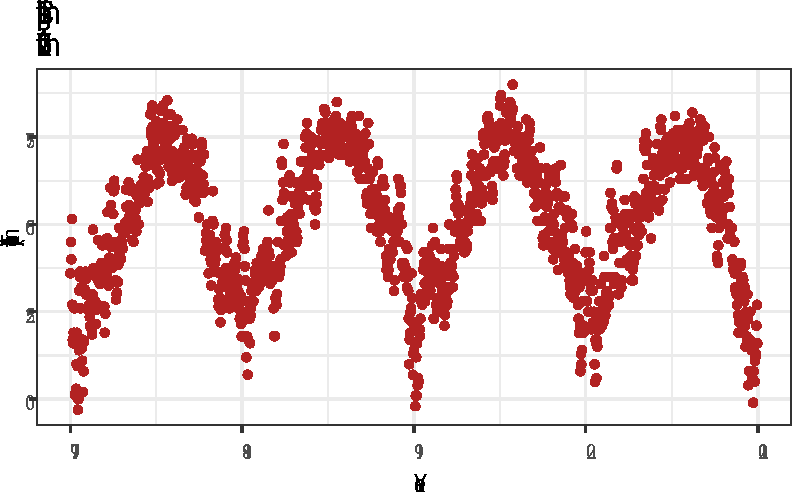
\includegraphics{ch5_files/figure-pdf/multiline-title-1.pdf}

Now You can Change fonts on the fly!

\begin{Shaded}
\begin{Highlighting}[]
\FunctionTok{ggplot}\NormalTok{(chic, }\FunctionTok{aes}\NormalTok{(}\AttributeTok{x =}\NormalTok{ date, }\AttributeTok{y =}\NormalTok{ temp)) }\SpecialCharTok{+}
    \FunctionTok{geom\_point}\NormalTok{(}\AttributeTok{color =} \StringTok{"firebrick"}\NormalTok{) }\SpecialCharTok{+}
    \FunctionTok{labs}\NormalTok{(}\AttributeTok{x =} \StringTok{"Year"}\NormalTok{, }\AttributeTok{y =} \StringTok{"Temperature (°F)"}\NormalTok{) }\SpecialCharTok{+}
    \FunctionTok{ggtitle}\NormalTok{(}\StringTok{"Temperatures in Chicago}\SpecialCharTok{\textbackslash{}n}\StringTok{from 1997 to 2001"}\NormalTok{) }\SpecialCharTok{+}
    \FunctionTok{theme\_bw}\NormalTok{(}\AttributeTok{base\_family =} \StringTok{"Berkshire Swash"}\NormalTok{)}
\end{Highlighting}
\end{Shaded}

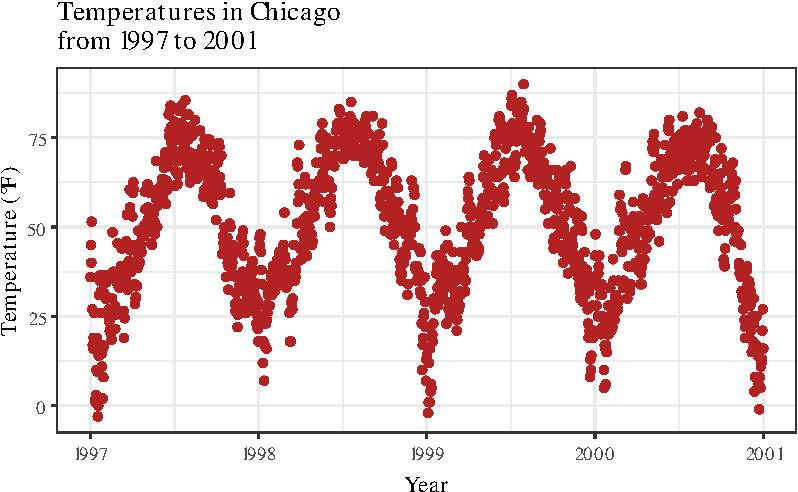
\includegraphics{ch5_files/figure-pdf/unnamed-chunk-1-1.pdf}

Or, Change it to Traditional \texttt{Times\ New\ Roman}:

\begin{Shaded}
\begin{Highlighting}[]
\FunctionTok{ggplot}\NormalTok{(chic, }\FunctionTok{aes}\NormalTok{(}\AttributeTok{x =}\NormalTok{ date, }\AttributeTok{y =}\NormalTok{ temp)) }\SpecialCharTok{+}
    \FunctionTok{geom\_point}\NormalTok{(}\AttributeTok{color =} \StringTok{"firebrick"}\NormalTok{) }\SpecialCharTok{+}
    \FunctionTok{labs}\NormalTok{(}\AttributeTok{x =} \StringTok{"Year"}\NormalTok{, }\AttributeTok{y =} \StringTok{"Temperature (°F)"}\NormalTok{) }\SpecialCharTok{+}
    \FunctionTok{ggtitle}\NormalTok{(}\StringTok{"Temperatures in Chicago}\SpecialCharTok{\textbackslash{}n}\StringTok{from 1997 to 2001"}\NormalTok{) }\SpecialCharTok{+}
    \FunctionTok{theme\_bw}\NormalTok{(}\AttributeTok{base\_family =} \StringTok{"Times New Roman"}\NormalTok{)}
\end{Highlighting}
\end{Shaded}

\begin{verbatim}
Warning in grid.Call(C_stringMetric, as.graphicsAnnot(x$label)): font metrics
unknown for character 0x4d
\end{verbatim}

\begin{verbatim}
Warning in grid.Call(C_stringMetric, as.graphicsAnnot(x$label)): font width
unknown for character 0x67
\end{verbatim}

\begin{verbatim}
Warning in grid.Call(C_stringMetric, as.graphicsAnnot(x$label)): font width
unknown for character 0x6a
\end{verbatim}

\begin{verbatim}
Warning in grid.Call(C_stringMetric, as.graphicsAnnot(x$label)): font width
unknown for character 0x70
\end{verbatim}

\begin{verbatim}
Warning in grid.Call(C_stringMetric, as.graphicsAnnot(x$label)): font width
unknown for character 0x71
\end{verbatim}

\begin{verbatim}
Warning in grid.Call(C_stringMetric, as.graphicsAnnot(x$label)): font width
unknown for character 0x79
\end{verbatim}

\begin{verbatim}
Warning in grid.Call(C_stringMetric, as.graphicsAnnot(x$label)): font width
unknown for character 0x51
\end{verbatim}

\begin{verbatim}
Warning in grid.Call(C_textBounds, as.graphicsAnnot(x$label), x$x, x$y, : font
width unknown for character 0x31
\end{verbatim}

\begin{verbatim}
Warning in grid.Call(C_textBounds, as.graphicsAnnot(x$label), x$x, x$y, : font
width unknown for character 0x39

Warning in grid.Call(C_textBounds, as.graphicsAnnot(x$label), x$x, x$y, : font
width unknown for character 0x39
\end{verbatim}

\begin{verbatim}
Warning in grid.Call(C_textBounds, as.graphicsAnnot(x$label), x$x, x$y, : font
width unknown for character 0x37
\end{verbatim}

\begin{verbatim}
Warning in grid.Call(C_textBounds, as.graphicsAnnot(x$label), x$x, x$y, : font
width unknown for character 0x31
\end{verbatim}

\begin{verbatim}
Warning in grid.Call(C_textBounds, as.graphicsAnnot(x$label), x$x, x$y, : font
width unknown for character 0x39

Warning in grid.Call(C_textBounds, as.graphicsAnnot(x$label), x$x, x$y, : font
width unknown for character 0x39
\end{verbatim}

\begin{verbatim}
Warning in grid.Call(C_textBounds, as.graphicsAnnot(x$label), x$x, x$y, : font
width unknown for character 0x38
\end{verbatim}

\begin{verbatim}
Warning in grid.Call(C_textBounds, as.graphicsAnnot(x$label), x$x, x$y, : font
width unknown for character 0x31
\end{verbatim}

\begin{verbatim}
Warning in grid.Call(C_textBounds, as.graphicsAnnot(x$label), x$x, x$y, : font
width unknown for character 0x39

Warning in grid.Call(C_textBounds, as.graphicsAnnot(x$label), x$x, x$y, : font
width unknown for character 0x39

Warning in grid.Call(C_textBounds, as.graphicsAnnot(x$label), x$x, x$y, : font
width unknown for character 0x39
\end{verbatim}

\begin{verbatim}
Warning in grid.Call(C_textBounds, as.graphicsAnnot(x$label), x$x, x$y, : font
width unknown for character 0x32
\end{verbatim}

\begin{verbatim}
Warning in grid.Call(C_textBounds, as.graphicsAnnot(x$label), x$x, x$y, : font
width unknown for character 0x30

Warning in grid.Call(C_textBounds, as.graphicsAnnot(x$label), x$x, x$y, : font
width unknown for character 0x30

Warning in grid.Call(C_textBounds, as.graphicsAnnot(x$label), x$x, x$y, : font
width unknown for character 0x30
\end{verbatim}

\begin{verbatim}
Warning in grid.Call(C_textBounds, as.graphicsAnnot(x$label), x$x, x$y, : font
width unknown for character 0x32
\end{verbatim}

\begin{verbatim}
Warning in grid.Call(C_textBounds, as.graphicsAnnot(x$label), x$x, x$y, : font
width unknown for character 0x30

Warning in grid.Call(C_textBounds, as.graphicsAnnot(x$label), x$x, x$y, : font
width unknown for character 0x30
\end{verbatim}

\begin{verbatim}
Warning in grid.Call(C_textBounds, as.graphicsAnnot(x$label), x$x, x$y, : font
width unknown for character 0x31
\end{verbatim}

\begin{verbatim}
Warning in grid.Call(C_textBounds, as.graphicsAnnot(x$label), x$x, x$y, : font
width unknown for character 0x30
\end{verbatim}

\begin{verbatim}
Warning in grid.Call(C_textBounds, as.graphicsAnnot(x$label), x$x, x$y, : font
width unknown for character 0x32
\end{verbatim}

\begin{verbatim}
Warning in grid.Call(C_textBounds, as.graphicsAnnot(x$label), x$x, x$y, : font
width unknown for character 0x35

Warning in grid.Call(C_textBounds, as.graphicsAnnot(x$label), x$x, x$y, : font
width unknown for character 0x35
\end{verbatim}

\begin{verbatim}
Warning in grid.Call(C_textBounds, as.graphicsAnnot(x$label), x$x, x$y, : font
width unknown for character 0x30
\end{verbatim}

\begin{verbatim}
Warning in grid.Call(C_textBounds, as.graphicsAnnot(x$label), x$x, x$y, : font
width unknown for character 0x37
\end{verbatim}

\begin{verbatim}
Warning in grid.Call(C_textBounds, as.graphicsAnnot(x$label), x$x, x$y, : font
width unknown for character 0x35
\end{verbatim}

\begin{verbatim}
Warning in grid.Call(C_stringMetric, as.graphicsAnnot(x$label)): font metrics
unknown for character 0x4d
\end{verbatim}

\begin{verbatim}
Warning in grid.Call(C_stringMetric, as.graphicsAnnot(x$label)): font width
unknown for character 0x67
\end{verbatim}

\begin{verbatim}
Warning in grid.Call(C_stringMetric, as.graphicsAnnot(x$label)): font width
unknown for character 0x6a
\end{verbatim}

\begin{verbatim}
Warning in grid.Call(C_stringMetric, as.graphicsAnnot(x$label)): font width
unknown for character 0x70
\end{verbatim}

\begin{verbatim}
Warning in grid.Call(C_stringMetric, as.graphicsAnnot(x$label)): font width
unknown for character 0x71
\end{verbatim}

\begin{verbatim}
Warning in grid.Call(C_stringMetric, as.graphicsAnnot(x$label)): font width
unknown for character 0x79
\end{verbatim}

\begin{verbatim}
Warning in grid.Call(C_stringMetric, as.graphicsAnnot(x$label)): font width
unknown for character 0x51
\end{verbatim}

\begin{verbatim}
Warning in grid.Call(C_stringMetric, as.graphicsAnnot(x$label)): font metrics
unknown for character 0x4d
\end{verbatim}

\begin{verbatim}
Warning in grid.Call(C_stringMetric, as.graphicsAnnot(x$label)): font width
unknown for character 0x67
\end{verbatim}

\begin{verbatim}
Warning in grid.Call(C_stringMetric, as.graphicsAnnot(x$label)): font width
unknown for character 0x6a
\end{verbatim}

\begin{verbatim}
Warning in grid.Call(C_stringMetric, as.graphicsAnnot(x$label)): font width
unknown for character 0x70
\end{verbatim}

\begin{verbatim}
Warning in grid.Call(C_stringMetric, as.graphicsAnnot(x$label)): font width
unknown for character 0x71
\end{verbatim}

\begin{verbatim}
Warning in grid.Call(C_stringMetric, as.graphicsAnnot(x$label)): font width
unknown for character 0x79
\end{verbatim}

\begin{verbatim}
Warning in grid.Call(C_stringMetric, as.graphicsAnnot(x$label)): font width
unknown for character 0x51
\end{verbatim}

\begin{verbatim}
Warning in grid.Call(C_textBounds, as.graphicsAnnot(x$label), x$x, x$y, : font
width unknown for character 0x54
\end{verbatim}

\begin{verbatim}
Warning in grid.Call(C_textBounds, as.graphicsAnnot(x$label), x$x, x$y, : font
width unknown for character 0xab
\end{verbatim}

\begin{verbatim}
Warning in grid.Call(C_textBounds, as.graphicsAnnot(x$label), x$x, x$y, : font
width unknown for character 0xcd
\end{verbatim}

\begin{verbatim}
Warning in grid.Call(C_textBounds, as.graphicsAnnot(x$label), x$x, x$y, : font
width unknown for character 0xf4
\end{verbatim}

\begin{verbatim}
Warning in grid.Call(C_textBounds, as.graphicsAnnot(x$label), x$x, x$y, : font
width unknown for character 0xfd
\end{verbatim}

\begin{verbatim}
Warning in grid.Call(C_textBounds, as.graphicsAnnot(x$label), x$x, x$y, : font
width unknown for character 0x7f
\end{verbatim}

\begin{verbatim}
Warning in grid.Call(C_textBounds, as.graphicsAnnot(x$label), x$x, x$y, : font
metrics unknown for character 0x4d
\end{verbatim}

\begin{verbatim}
Warning in grid.Call(C_textBounds, as.graphicsAnnot(x$label), x$x, x$y, : font
width unknown for character 0x54
\end{verbatim}

\begin{verbatim}
Warning in grid.Call(C_textBounds, as.graphicsAnnot(x$label), x$x, x$y, : font
width unknown for character 0x65
\end{verbatim}

\begin{verbatim}
Warning in grid.Call(C_textBounds, as.graphicsAnnot(x$label), x$x, x$y, : font
width unknown for character 0x6d
\end{verbatim}

\begin{verbatim}
Warning in grid.Call(C_textBounds, as.graphicsAnnot(x$label), x$x, x$y, : font
width unknown for character 0x70
\end{verbatim}

\begin{verbatim}
Warning in grid.Call(C_textBounds, as.graphicsAnnot(x$label), x$x, x$y, : font
width unknown for character 0x65
\end{verbatim}

\begin{verbatim}
Warning in grid.Call(C_textBounds, as.graphicsAnnot(x$label), x$x, x$y, : font
width unknown for character 0x72
\end{verbatim}

\begin{verbatim}
Warning in grid.Call(C_textBounds, as.graphicsAnnot(x$label), x$x, x$y, : font
width unknown for character 0x61
\end{verbatim}

\begin{verbatim}
Warning in grid.Call(C_textBounds, as.graphicsAnnot(x$label), x$x, x$y, : font
width unknown for character 0x74
\end{verbatim}

\begin{verbatim}
Warning in grid.Call(C_textBounds, as.graphicsAnnot(x$label), x$x, x$y, : font
width unknown for character 0x75
\end{verbatim}

\begin{verbatim}
Warning in grid.Call(C_textBounds, as.graphicsAnnot(x$label), x$x, x$y, : font
width unknown for character 0x72
\end{verbatim}

\begin{verbatim}
Warning in grid.Call(C_textBounds, as.graphicsAnnot(x$label), x$x, x$y, : font
width unknown for character 0x65
\end{verbatim}

\begin{verbatim}
Warning in grid.Call(C_textBounds, as.graphicsAnnot(x$label), x$x, x$y, : font
width unknown for character 0x73
\end{verbatim}

\begin{verbatim}
Warning in grid.Call(C_textBounds, as.graphicsAnnot(x$label), x$x, x$y, : font
width unknown for character 0x20
\end{verbatim}

\begin{verbatim}
Warning in grid.Call(C_textBounds, as.graphicsAnnot(x$label), x$x, x$y, : font
width unknown for character 0x69
\end{verbatim}

\begin{verbatim}
Warning in grid.Call(C_textBounds, as.graphicsAnnot(x$label), x$x, x$y, : font
width unknown for character 0x6e
\end{verbatim}

\begin{verbatim}
Warning in grid.Call(C_textBounds, as.graphicsAnnot(x$label), x$x, x$y, : font
width unknown for character 0x20
\end{verbatim}

\begin{verbatim}
Warning in grid.Call(C_textBounds, as.graphicsAnnot(x$label), x$x, x$y, : font
width unknown for character 0x43
\end{verbatim}

\begin{verbatim}
Warning in grid.Call(C_textBounds, as.graphicsAnnot(x$label), x$x, x$y, : font
width unknown for character 0x68
\end{verbatim}

\begin{verbatim}
Warning in grid.Call(C_textBounds, as.graphicsAnnot(x$label), x$x, x$y, : font
width unknown for character 0x69
\end{verbatim}

\begin{verbatim}
Warning in grid.Call(C_textBounds, as.graphicsAnnot(x$label), x$x, x$y, : font
width unknown for character 0x63
\end{verbatim}

\begin{verbatim}
Warning in grid.Call(C_textBounds, as.graphicsAnnot(x$label), x$x, x$y, : font
width unknown for character 0x61
\end{verbatim}

\begin{verbatim}
Warning in grid.Call(C_textBounds, as.graphicsAnnot(x$label), x$x, x$y, : font
width unknown for character 0x67
\end{verbatim}

\begin{verbatim}
Warning in grid.Call(C_textBounds, as.graphicsAnnot(x$label), x$x, x$y, : font
width unknown for character 0x6f
\end{verbatim}

\begin{verbatim}
Warning in grid.Call(C_textBounds, as.graphicsAnnot(x$label), x$x, x$y, : font
width unknown for character 0x66
\end{verbatim}

\begin{verbatim}
Warning in grid.Call(C_textBounds, as.graphicsAnnot(x$label), x$x, x$y, : font
width unknown for character 0x72
\end{verbatim}

\begin{verbatim}
Warning in grid.Call(C_textBounds, as.graphicsAnnot(x$label), x$x, x$y, : font
width unknown for character 0x6f
\end{verbatim}

\begin{verbatim}
Warning in grid.Call(C_textBounds, as.graphicsAnnot(x$label), x$x, x$y, : font
width unknown for character 0x6d
\end{verbatim}

\begin{verbatim}
Warning in grid.Call(C_textBounds, as.graphicsAnnot(x$label), x$x, x$y, : font
width unknown for character 0x20
\end{verbatim}

\begin{verbatim}
Warning in grid.Call(C_textBounds, as.graphicsAnnot(x$label), x$x, x$y, : font
width unknown for character 0x31
\end{verbatim}

\begin{verbatim}
Warning in grid.Call(C_textBounds, as.graphicsAnnot(x$label), x$x, x$y, : font
width unknown for character 0x39

Warning in grid.Call(C_textBounds, as.graphicsAnnot(x$label), x$x, x$y, : font
width unknown for character 0x39
\end{verbatim}

\begin{verbatim}
Warning in grid.Call(C_textBounds, as.graphicsAnnot(x$label), x$x, x$y, : font
width unknown for character 0x37
\end{verbatim}

\begin{verbatim}
Warning in grid.Call(C_textBounds, as.graphicsAnnot(x$label), x$x, x$y, : font
width unknown for character 0x20
\end{verbatim}

\begin{verbatim}
Warning in grid.Call(C_textBounds, as.graphicsAnnot(x$label), x$x, x$y, : font
width unknown for character 0x74
\end{verbatim}

\begin{verbatim}
Warning in grid.Call(C_textBounds, as.graphicsAnnot(x$label), x$x, x$y, : font
width unknown for character 0x6f
\end{verbatim}

\begin{verbatim}
Warning in grid.Call(C_textBounds, as.graphicsAnnot(x$label), x$x, x$y, : font
width unknown for character 0x20
\end{verbatim}

\begin{verbatim}
Warning in grid.Call(C_textBounds, as.graphicsAnnot(x$label), x$x, x$y, : font
width unknown for character 0x32
\end{verbatim}

\begin{verbatim}
Warning in grid.Call(C_textBounds, as.graphicsAnnot(x$label), x$x, x$y, : font
width unknown for character 0x30

Warning in grid.Call(C_textBounds, as.graphicsAnnot(x$label), x$x, x$y, : font
width unknown for character 0x30
\end{verbatim}

\begin{verbatim}
Warning in grid.Call(C_textBounds, as.graphicsAnnot(x$label), x$x, x$y, : font
width unknown for character 0x31
\end{verbatim}

\begin{verbatim}
Warning in grid.Call(C_textBounds, as.graphicsAnnot(x$label), x$x, x$y, : font
metrics unknown for character 0x4d
\end{verbatim}

\begin{verbatim}
Warning in grid.Call(C_textBounds, as.graphicsAnnot(x$label), x$x, x$y, : font
width unknown for character 0x59
\end{verbatim}

\begin{verbatim}
Warning in grid.Call(C_textBounds, as.graphicsAnnot(x$label), x$x, x$y, : font
width unknown for character 0x65
\end{verbatim}

\begin{verbatim}
Warning in grid.Call(C_textBounds, as.graphicsAnnot(x$label), x$x, x$y, : font
width unknown for character 0x61
\end{verbatim}

\begin{verbatim}
Warning in grid.Call(C_textBounds, as.graphicsAnnot(x$label), x$x, x$y, : font
width unknown for character 0x72
\end{verbatim}

\begin{verbatim}
Warning in grid.Call(C_textBounds, as.graphicsAnnot(x$label), x$x, x$y, : font
metrics unknown for character 0x4d
\end{verbatim}

\begin{verbatim}
Warning in grid.Call.graphics(C_text, as.graphicsAnnot(x$label), x$x, x$y, :
font width unknown for character 0x30
\end{verbatim}

\begin{verbatim}
Warning in grid.Call.graphics(C_text, as.graphicsAnnot(x$label), x$x, x$y, :
font metrics unknown for character 0x4d
\end{verbatim}

\begin{verbatim}
Warning in grid.Call.graphics(C_text, as.graphicsAnnot(x$label), x$x, x$y, :
font width unknown for character 0x32
\end{verbatim}

\begin{verbatim}
Warning in grid.Call.graphics(C_text, as.graphicsAnnot(x$label), x$x, x$y, :
font width unknown for character 0x35

Warning in grid.Call.graphics(C_text, as.graphicsAnnot(x$label), x$x, x$y, :
font width unknown for character 0x35
\end{verbatim}

\begin{verbatim}
Warning in grid.Call.graphics(C_text, as.graphicsAnnot(x$label), x$x, x$y, :
font width unknown for character 0x30
\end{verbatim}

\begin{verbatim}
Warning in grid.Call.graphics(C_text, as.graphicsAnnot(x$label), x$x, x$y, :
font width unknown for character 0x37
\end{verbatim}

\begin{verbatim}
Warning in grid.Call.graphics(C_text, as.graphicsAnnot(x$label), x$x, x$y, :
font width unknown for character 0x35
\end{verbatim}

\begin{verbatim}
Warning in grid.Call.graphics(C_text, as.graphicsAnnot(x$label), x$x, x$y, :
font width unknown for character 0x31
\end{verbatim}

\begin{verbatim}
Warning in grid.Call.graphics(C_text, as.graphicsAnnot(x$label), x$x, x$y, :
font width unknown for character 0x39

Warning in grid.Call.graphics(C_text, as.graphicsAnnot(x$label), x$x, x$y, :
font width unknown for character 0x39
\end{verbatim}

\begin{verbatim}
Warning in grid.Call.graphics(C_text, as.graphicsAnnot(x$label), x$x, x$y, :
font width unknown for character 0x37
\end{verbatim}

\begin{verbatim}
Warning in grid.Call.graphics(C_text, as.graphicsAnnot(x$label), x$x, x$y, :
font width unknown for character 0x31
\end{verbatim}

\begin{verbatim}
Warning in grid.Call.graphics(C_text, as.graphicsAnnot(x$label), x$x, x$y, :
font width unknown for character 0x39

Warning in grid.Call.graphics(C_text, as.graphicsAnnot(x$label), x$x, x$y, :
font width unknown for character 0x39
\end{verbatim}

\begin{verbatim}
Warning in grid.Call.graphics(C_text, as.graphicsAnnot(x$label), x$x, x$y, :
font width unknown for character 0x38
\end{verbatim}

\begin{verbatim}
Warning in grid.Call.graphics(C_text, as.graphicsAnnot(x$label), x$x, x$y, :
font width unknown for character 0x31
\end{verbatim}

\begin{verbatim}
Warning in grid.Call.graphics(C_text, as.graphicsAnnot(x$label), x$x, x$y, :
font width unknown for character 0x39

Warning in grid.Call.graphics(C_text, as.graphicsAnnot(x$label), x$x, x$y, :
font width unknown for character 0x39

Warning in grid.Call.graphics(C_text, as.graphicsAnnot(x$label), x$x, x$y, :
font width unknown for character 0x39
\end{verbatim}

\begin{verbatim}
Warning in grid.Call.graphics(C_text, as.graphicsAnnot(x$label), x$x, x$y, :
font width unknown for character 0x32
\end{verbatim}

\begin{verbatim}
Warning in grid.Call.graphics(C_text, as.graphicsAnnot(x$label), x$x, x$y, :
font width unknown for character 0x30

Warning in grid.Call.graphics(C_text, as.graphicsAnnot(x$label), x$x, x$y, :
font width unknown for character 0x30

Warning in grid.Call.graphics(C_text, as.graphicsAnnot(x$label), x$x, x$y, :
font width unknown for character 0x30
\end{verbatim}

\begin{verbatim}
Warning in grid.Call.graphics(C_text, as.graphicsAnnot(x$label), x$x, x$y, :
font width unknown for character 0x32
\end{verbatim}

\begin{verbatim}
Warning in grid.Call.graphics(C_text, as.graphicsAnnot(x$label), x$x, x$y, :
font width unknown for character 0x30

Warning in grid.Call.graphics(C_text, as.graphicsAnnot(x$label), x$x, x$y, :
font width unknown for character 0x30
\end{verbatim}

\begin{verbatim}
Warning in grid.Call.graphics(C_text, as.graphicsAnnot(x$label), x$x, x$y, :
font width unknown for character 0x31
\end{verbatim}

\begin{verbatim}
Warning in grid.Call.graphics(C_text, as.graphicsAnnot(x$label), x$x, x$y, :
font width unknown for character 0x59
\end{verbatim}

\begin{verbatim}
Warning in grid.Call.graphics(C_text, as.graphicsAnnot(x$label), x$x, x$y, :
font width unknown for character 0x65
\end{verbatim}

\begin{verbatim}
Warning in grid.Call.graphics(C_text, as.graphicsAnnot(x$label), x$x, x$y, :
font width unknown for character 0x61
\end{verbatim}

\begin{verbatim}
Warning in grid.Call.graphics(C_text, as.graphicsAnnot(x$label), x$x, x$y, :
font width unknown for character 0x72
\end{verbatim}

\begin{verbatim}
Warning in grid.Call.graphics(C_text, as.graphicsAnnot(x$label), x$x, x$y, :
font metrics unknown for character 0x4d
\end{verbatim}

\begin{verbatim}
Warning in grid.Call.graphics(C_text, as.graphicsAnnot(x$label), x$x, x$y, :
font width unknown for character 0x54
\end{verbatim}

\begin{verbatim}
Warning in grid.Call.graphics(C_text, as.graphicsAnnot(x$label), x$x, x$y, :
font width unknown for character 0xab
\end{verbatim}

\begin{verbatim}
Warning in grid.Call.graphics(C_text, as.graphicsAnnot(x$label), x$x, x$y, :
font width unknown for character 0xcd
\end{verbatim}

\begin{verbatim}
Warning in grid.Call.graphics(C_text, as.graphicsAnnot(x$label), x$x, x$y, :
font width unknown for character 0xf4
\end{verbatim}

\begin{verbatim}
Warning in grid.Call.graphics(C_text, as.graphicsAnnot(x$label), x$x, x$y, :
font width unknown for character 0xfd
\end{verbatim}

\begin{verbatim}
Warning in grid.Call.graphics(C_text, as.graphicsAnnot(x$label), x$x, x$y, :
font width unknown for character 0x7f
\end{verbatim}

\begin{verbatim}
Warning in grid.Call.graphics(C_text, as.graphicsAnnot(x$label), x$x, x$y, :
font width unknown for character 0x54
\end{verbatim}

\begin{verbatim}
Warning in grid.Call.graphics(C_text, as.graphicsAnnot(x$label), x$x, x$y, :
font width unknown for character 0x65
\end{verbatim}

\begin{verbatim}
Warning in grid.Call.graphics(C_text, as.graphicsAnnot(x$label), x$x, x$y, :
font width unknown for character 0x6d
\end{verbatim}

\begin{verbatim}
Warning in grid.Call.graphics(C_text, as.graphicsAnnot(x$label), x$x, x$y, :
font width unknown for character 0x70
\end{verbatim}

\begin{verbatim}
Warning in grid.Call.graphics(C_text, as.graphicsAnnot(x$label), x$x, x$y, :
font width unknown for character 0x65
\end{verbatim}

\begin{verbatim}
Warning in grid.Call.graphics(C_text, as.graphicsAnnot(x$label), x$x, x$y, :
font width unknown for character 0x72
\end{verbatim}

\begin{verbatim}
Warning in grid.Call.graphics(C_text, as.graphicsAnnot(x$label), x$x, x$y, :
font width unknown for character 0x61
\end{verbatim}

\begin{verbatim}
Warning in grid.Call.graphics(C_text, as.graphicsAnnot(x$label), x$x, x$y, :
font width unknown for character 0x74
\end{verbatim}

\begin{verbatim}
Warning in grid.Call.graphics(C_text, as.graphicsAnnot(x$label), x$x, x$y, :
font width unknown for character 0x75
\end{verbatim}

\begin{verbatim}
Warning in grid.Call.graphics(C_text, as.graphicsAnnot(x$label), x$x, x$y, :
font width unknown for character 0x72
\end{verbatim}

\begin{verbatim}
Warning in grid.Call.graphics(C_text, as.graphicsAnnot(x$label), x$x, x$y, :
font width unknown for character 0x65
\end{verbatim}

\begin{verbatim}
Warning in grid.Call.graphics(C_text, as.graphicsAnnot(x$label), x$x, x$y, :
font width unknown for character 0x73
\end{verbatim}

\begin{verbatim}
Warning in grid.Call.graphics(C_text, as.graphicsAnnot(x$label), x$x, x$y, :
font width unknown for character 0x20
\end{verbatim}

\begin{verbatim}
Warning in grid.Call.graphics(C_text, as.graphicsAnnot(x$label), x$x, x$y, :
font width unknown for character 0x69
\end{verbatim}

\begin{verbatim}
Warning in grid.Call.graphics(C_text, as.graphicsAnnot(x$label), x$x, x$y, :
font width unknown for character 0x6e
\end{verbatim}

\begin{verbatim}
Warning in grid.Call.graphics(C_text, as.graphicsAnnot(x$label), x$x, x$y, :
font width unknown for character 0x20
\end{verbatim}

\begin{verbatim}
Warning in grid.Call.graphics(C_text, as.graphicsAnnot(x$label), x$x, x$y, :
font width unknown for character 0x43
\end{verbatim}

\begin{verbatim}
Warning in grid.Call.graphics(C_text, as.graphicsAnnot(x$label), x$x, x$y, :
font width unknown for character 0x68
\end{verbatim}

\begin{verbatim}
Warning in grid.Call.graphics(C_text, as.graphicsAnnot(x$label), x$x, x$y, :
font width unknown for character 0x69
\end{verbatim}

\begin{verbatim}
Warning in grid.Call.graphics(C_text, as.graphicsAnnot(x$label), x$x, x$y, :
font width unknown for character 0x63
\end{verbatim}

\begin{verbatim}
Warning in grid.Call.graphics(C_text, as.graphicsAnnot(x$label), x$x, x$y, :
font width unknown for character 0x61
\end{verbatim}

\begin{verbatim}
Warning in grid.Call.graphics(C_text, as.graphicsAnnot(x$label), x$x, x$y, :
font width unknown for character 0x67
\end{verbatim}

\begin{verbatim}
Warning in grid.Call.graphics(C_text, as.graphicsAnnot(x$label), x$x, x$y, :
font width unknown for character 0x6f
\end{verbatim}

\begin{verbatim}
Warning in grid.Call.graphics(C_text, as.graphicsAnnot(x$label), x$x, x$y, :
font metrics unknown for character 0x4d
\end{verbatim}

\begin{verbatim}
Warning in grid.Call.graphics(C_text, as.graphicsAnnot(x$label), x$x, x$y, :
font width unknown for character 0x66
\end{verbatim}

\begin{verbatim}
Warning in grid.Call.graphics(C_text, as.graphicsAnnot(x$label), x$x, x$y, :
font width unknown for character 0x72
\end{verbatim}

\begin{verbatim}
Warning in grid.Call.graphics(C_text, as.graphicsAnnot(x$label), x$x, x$y, :
font width unknown for character 0x6f
\end{verbatim}

\begin{verbatim}
Warning in grid.Call.graphics(C_text, as.graphicsAnnot(x$label), x$x, x$y, :
font width unknown for character 0x6d
\end{verbatim}

\begin{verbatim}
Warning in grid.Call.graphics(C_text, as.graphicsAnnot(x$label), x$x, x$y, :
font width unknown for character 0x20
\end{verbatim}

\begin{verbatim}
Warning in grid.Call.graphics(C_text, as.graphicsAnnot(x$label), x$x, x$y, :
font width unknown for character 0x31
\end{verbatim}

\begin{verbatim}
Warning in grid.Call.graphics(C_text, as.graphicsAnnot(x$label), x$x, x$y, :
font width unknown for character 0x39

Warning in grid.Call.graphics(C_text, as.graphicsAnnot(x$label), x$x, x$y, :
font width unknown for character 0x39
\end{verbatim}

\begin{verbatim}
Warning in grid.Call.graphics(C_text, as.graphicsAnnot(x$label), x$x, x$y, :
font width unknown for character 0x37
\end{verbatim}

\begin{verbatim}
Warning in grid.Call.graphics(C_text, as.graphicsAnnot(x$label), x$x, x$y, :
font width unknown for character 0x20
\end{verbatim}

\begin{verbatim}
Warning in grid.Call.graphics(C_text, as.graphicsAnnot(x$label), x$x, x$y, :
font width unknown for character 0x74
\end{verbatim}

\begin{verbatim}
Warning in grid.Call.graphics(C_text, as.graphicsAnnot(x$label), x$x, x$y, :
font width unknown for character 0x6f
\end{verbatim}

\begin{verbatim}
Warning in grid.Call.graphics(C_text, as.graphicsAnnot(x$label), x$x, x$y, :
font width unknown for character 0x20
\end{verbatim}

\begin{verbatim}
Warning in grid.Call.graphics(C_text, as.graphicsAnnot(x$label), x$x, x$y, :
font width unknown for character 0x32
\end{verbatim}

\begin{verbatim}
Warning in grid.Call.graphics(C_text, as.graphicsAnnot(x$label), x$x, x$y, :
font width unknown for character 0x30

Warning in grid.Call.graphics(C_text, as.graphicsAnnot(x$label), x$x, x$y, :
font width unknown for character 0x30
\end{verbatim}

\begin{verbatim}
Warning in grid.Call.graphics(C_text, as.graphicsAnnot(x$label), x$x, x$y, :
font width unknown for character 0x31
\end{verbatim}

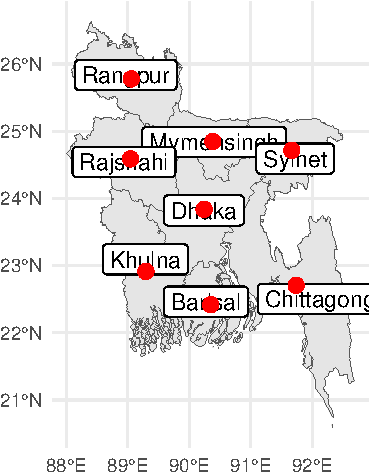
\includegraphics{ch5_files/figure-pdf/unnamed-chunk-2-1.pdf}

\bookmarksetup{startatroot}

\chapter{Working with Legends}\label{legends}

\begin{center}\rule{0.5\linewidth}{0.5pt}\end{center}

In this section, we will color code the plot based on the season. Or, to
phrase it more in the style of ggplot: we'll map the variable
\texttt{season} to the aesthetic \texttt{color}. One of the advantages
of \texttt{\{ggplot2\}} is that it automatically adds a legend when
mapping a variable to an aesthetic. As a result, the legend title
defaults to what we specified in the color argument:

\begin{Shaded}
\begin{Highlighting}[]
\FunctionTok{ggplot}\NormalTok{(chic,}
       \FunctionTok{aes}\NormalTok{(}\AttributeTok{x =}\NormalTok{ date, }\AttributeTok{y =}\NormalTok{ temp, }\AttributeTok{color =}\NormalTok{ season)) }\SpecialCharTok{+}
  \FunctionTok{geom\_point}\NormalTok{() }\SpecialCharTok{+}
  \FunctionTok{labs}\NormalTok{(}\AttributeTok{x =} \StringTok{"Year"}\NormalTok{, }\AttributeTok{y =} \StringTok{"Temperature (°F)"}\NormalTok{)}
\end{Highlighting}
\end{Shaded}

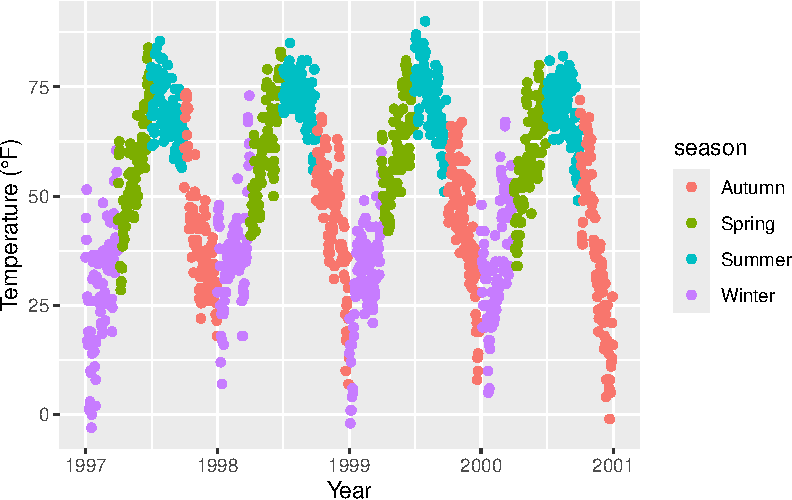
\includegraphics{ch6_files/figure-pdf/legend-default-1.pdf}

\section{Disabling the Legend}\label{disabling-the-legend}

One of the most common questions is: ``How do I remove the legend?''

It's quite straightforward and always effective with
\texttt{theme(legend.position\ =\ "none")}:

\begin{Shaded}
\begin{Highlighting}[]
\FunctionTok{ggplot}\NormalTok{(chic,}
       \FunctionTok{aes}\NormalTok{(}\AttributeTok{x =}\NormalTok{ date, }\AttributeTok{y =}\NormalTok{ temp, }\AttributeTok{color =}\NormalTok{ season)) }\SpecialCharTok{+}
  \FunctionTok{geom\_point}\NormalTok{() }\SpecialCharTok{+}
  \FunctionTok{labs}\NormalTok{(}\AttributeTok{x =} \StringTok{"Year"}\NormalTok{, }\AttributeTok{y =} \StringTok{"Temperature (°F)"}\NormalTok{) }\SpecialCharTok{+}
  \FunctionTok{theme}\NormalTok{(}\AttributeTok{legend.position =} \StringTok{"none"}\NormalTok{)}
\end{Highlighting}
\end{Shaded}

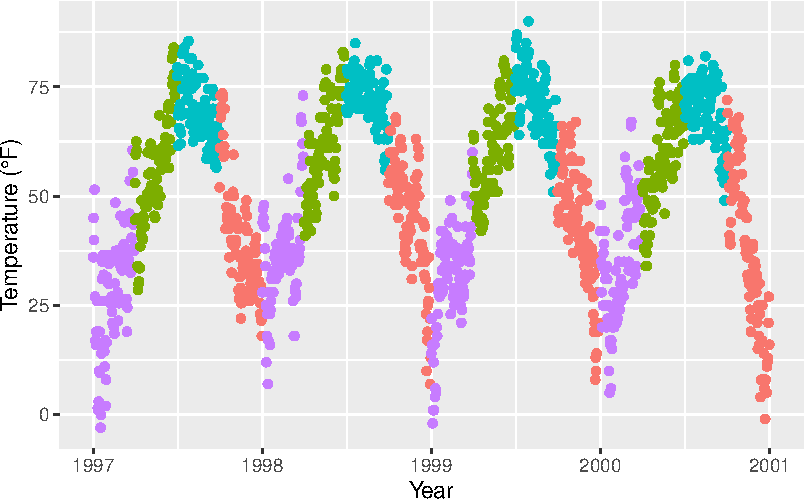
\includegraphics{ch6_files/figure-pdf/legend-none-1.pdf}

You can also utilize \texttt{guides(color\ =\ "none")} or
\texttt{scale\_color\_discrete(guide\ =\ "none")}, depending on the
specific case. While altering the theme element removes all legends at
once, you can selectively remove specific legends using the latter
options while keeping others:

\begin{Shaded}
\begin{Highlighting}[]
\FunctionTok{ggplot}\NormalTok{(chic,}
       \FunctionTok{aes}\NormalTok{(}\AttributeTok{x =}\NormalTok{ date, }\AttributeTok{y =}\NormalTok{ temp,}
           \AttributeTok{color =}\NormalTok{ season, }\AttributeTok{shape =}\NormalTok{ season)) }\SpecialCharTok{+}
  \FunctionTok{geom\_point}\NormalTok{() }\SpecialCharTok{+}
  \FunctionTok{labs}\NormalTok{(}\AttributeTok{x =} \StringTok{"Year"}\NormalTok{, }\AttributeTok{y =} \StringTok{"Temperature (°F)"}\NormalTok{) }\SpecialCharTok{+}
  \FunctionTok{guides}\NormalTok{(}\AttributeTok{color =} \StringTok{"none"}\NormalTok{)}
\end{Highlighting}
\end{Shaded}

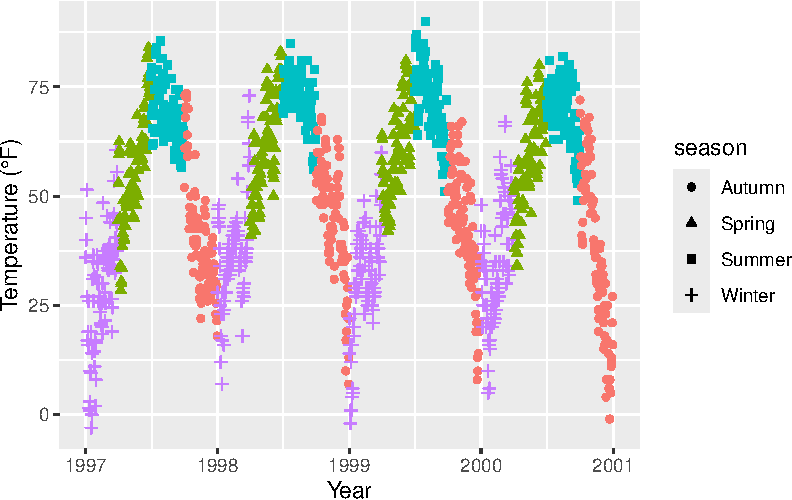
\includegraphics{ch6_files/figure-pdf/legend-none-guides-1.pdf}

Here, for example, we retain the legend for the shapes while discarding
the one for the colors.

\section{Eliminating Legend Titles}\label{eliminating-legend-titles}

As we've previously learned, utilize \texttt{element\_blank()} to render
\emph{nothing}:

\begin{Shaded}
\begin{Highlighting}[]
\FunctionTok{ggplot}\NormalTok{(chic, }\FunctionTok{aes}\NormalTok{(}\AttributeTok{x =}\NormalTok{ date, }\AttributeTok{y =}\NormalTok{ temp, }\AttributeTok{color =}\NormalTok{ season)) }\SpecialCharTok{+}
  \FunctionTok{geom\_point}\NormalTok{() }\SpecialCharTok{+}
  \FunctionTok{labs}\NormalTok{(}\AttributeTok{x =} \StringTok{"Year"}\NormalTok{, }\AttributeTok{y =} \StringTok{"Temperature (°F)"}\NormalTok{) }\SpecialCharTok{+}
  \FunctionTok{theme}\NormalTok{(}\AttributeTok{legend.title =} \FunctionTok{element\_blank}\NormalTok{())}
\end{Highlighting}
\end{Shaded}

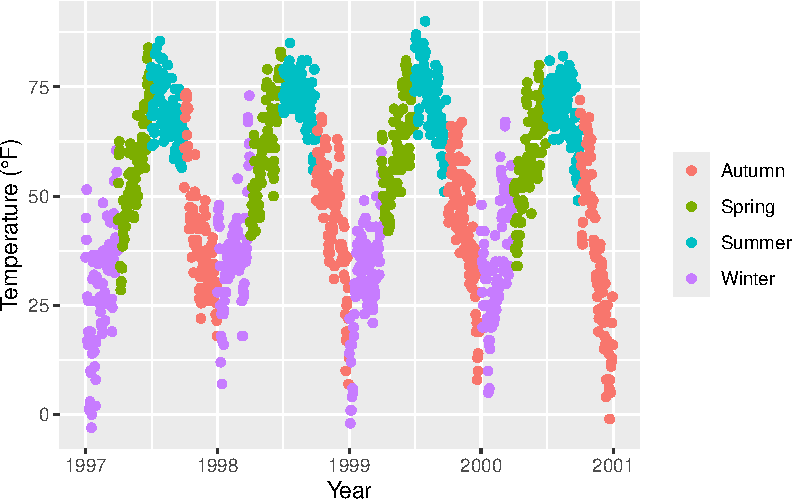
\includegraphics{ch6_files/figure-pdf/legend-title-off-1.pdf}

💁 You can achieve the same outcome by setting the legend name to
\texttt{NULL}, either through
\texttt{scale\_color\_discrete(name\ =\ NULL)} or
\texttt{labs(color\ =\ NULL)}. Expand to see examples.

\begin{Shaded}
\begin{Highlighting}[]
\FunctionTok{ggplot}\NormalTok{(chic, }\FunctionTok{aes}\NormalTok{(}\AttributeTok{x =}\NormalTok{ date, }\AttributeTok{y =}\NormalTok{ temp, }\AttributeTok{color =}\NormalTok{ season)) }\SpecialCharTok{+}
  \FunctionTok{geom\_point}\NormalTok{() }\SpecialCharTok{+}
  \FunctionTok{labs}\NormalTok{(}\AttributeTok{x =} \StringTok{"Year"}\NormalTok{, }\AttributeTok{y =} \StringTok{"Temperature (°F)"}\NormalTok{) }\SpecialCharTok{+}
  \FunctionTok{scale\_color\_discrete}\NormalTok{(}\AttributeTok{name =} \ConstantTok{NULL}\NormalTok{)}
\end{Highlighting}
\end{Shaded}

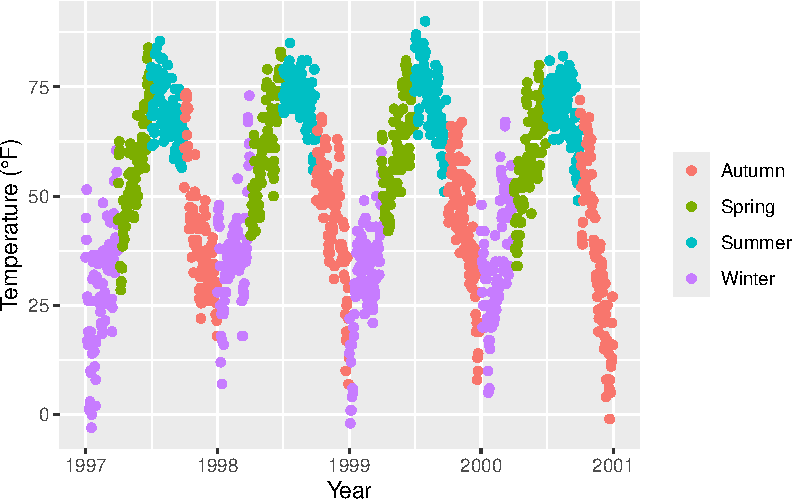
\includegraphics{ch6_files/figure-pdf/legend-title-null-1.pdf}

\begin{Shaded}
\begin{Highlighting}[]
\FunctionTok{ggplot}\NormalTok{(chic, }\FunctionTok{aes}\NormalTok{(}\AttributeTok{x =}\NormalTok{ date, }\AttributeTok{y =}\NormalTok{ temp, }\AttributeTok{color =}\NormalTok{ season)) }\SpecialCharTok{+}
  \FunctionTok{geom\_point}\NormalTok{() }\SpecialCharTok{+}
  \FunctionTok{labs}\NormalTok{(}\AttributeTok{x =} \StringTok{"Year"}\NormalTok{, }\AttributeTok{y =} \StringTok{"Temperature (°F)"}\NormalTok{) }\SpecialCharTok{+}
  \FunctionTok{labs}\NormalTok{(}\AttributeTok{color =} \ConstantTok{NULL}\NormalTok{)}
\end{Highlighting}
\end{Shaded}

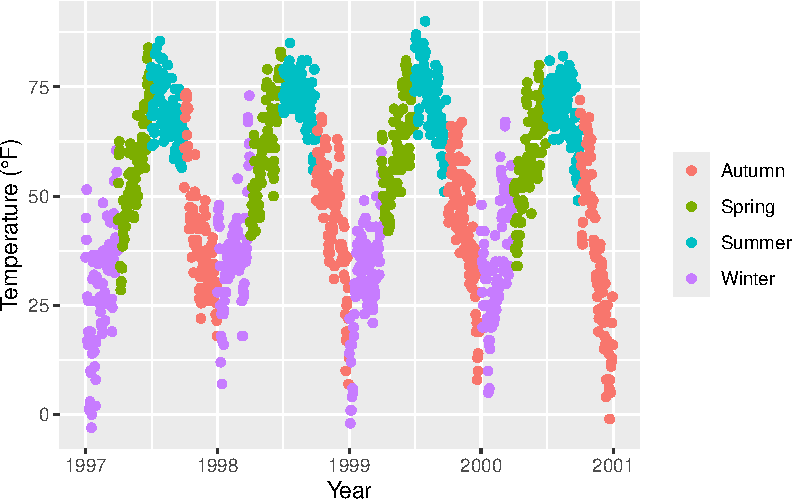
\includegraphics{ch6_files/figure-pdf/legend-title-labs-null-1.pdf}

\section{Adjusting Legend Position}\label{adjusting-legend-position}

To relocate the legend from its default position on the right side, you
can use the \texttt{legend.position} argument within \texttt{theme}.
Available positions include ``top'', ``right'' (the default),
``bottom'', and ``left''.

\begin{Shaded}
\begin{Highlighting}[]
\FunctionTok{ggplot}\NormalTok{(chic, }\FunctionTok{aes}\NormalTok{(}\AttributeTok{x =}\NormalTok{ date, }\AttributeTok{y =}\NormalTok{ temp, }\AttributeTok{color =}\NormalTok{ season)) }\SpecialCharTok{+}
  \FunctionTok{geom\_point}\NormalTok{() }\SpecialCharTok{+}
  \FunctionTok{labs}\NormalTok{(}\AttributeTok{x =} \StringTok{"Year"}\NormalTok{, }\AttributeTok{y =} \StringTok{"Temperature (°F)"}\NormalTok{) }\SpecialCharTok{+}
  \FunctionTok{theme}\NormalTok{(}\AttributeTok{legend.position =} \StringTok{"top"}\NormalTok{)}
\end{Highlighting}
\end{Shaded}

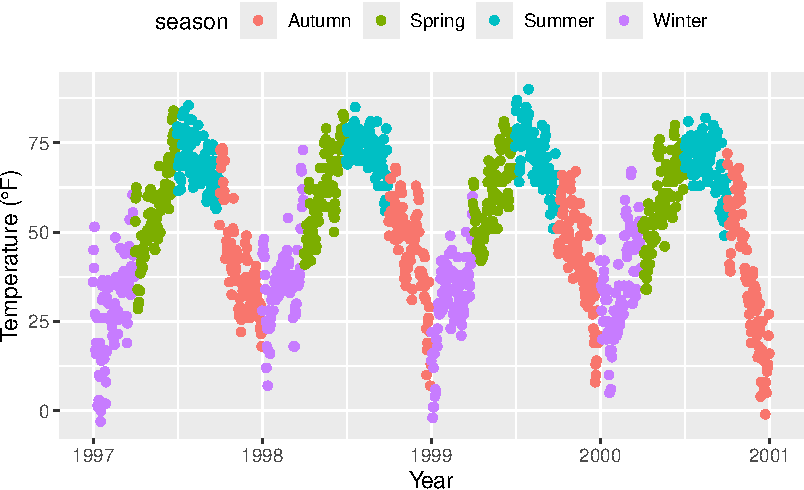
\includegraphics{ch6_files/figure-pdf/legend-top-1.pdf}

You can also position the legend inside the panel by specifying a vector
with relative \texttt{x} and \texttt{y} coordinates ranging from 0 (left
or bottom) to 1 (right or top):

\begin{Shaded}
\begin{Highlighting}[]
\FunctionTok{ggplot}\NormalTok{(chic, }\FunctionTok{aes}\NormalTok{(}\AttributeTok{x =}\NormalTok{ date, }\AttributeTok{y =}\NormalTok{ temp, }\AttributeTok{color =}\NormalTok{ season)) }\SpecialCharTok{+}
  \FunctionTok{geom\_point}\NormalTok{() }\SpecialCharTok{+}
  \FunctionTok{labs}\NormalTok{(}\AttributeTok{x =} \StringTok{"Year"}\NormalTok{, }\AttributeTok{y =} \StringTok{"Temperature (°F)"}\NormalTok{,}
       \AttributeTok{color =} \ConstantTok{NULL}\NormalTok{) }\SpecialCharTok{+}
  \FunctionTok{theme}\NormalTok{(}\AttributeTok{legend.position =} \FunctionTok{c}\NormalTok{(.}\DecValTok{15}\NormalTok{, .}\DecValTok{15}\NormalTok{),}
        \AttributeTok{legend.background =} \FunctionTok{element\_rect}\NormalTok{(}\AttributeTok{fill =} \StringTok{"transparent"}\NormalTok{))}
\end{Highlighting}
\end{Shaded}

\begin{verbatim}
Warning: A numeric `legend.position` argument in `theme()` was deprecated in ggplot2
3.5.0.
i Please use the `legend.position.inside` argument of `theme()` instead.
\end{verbatim}

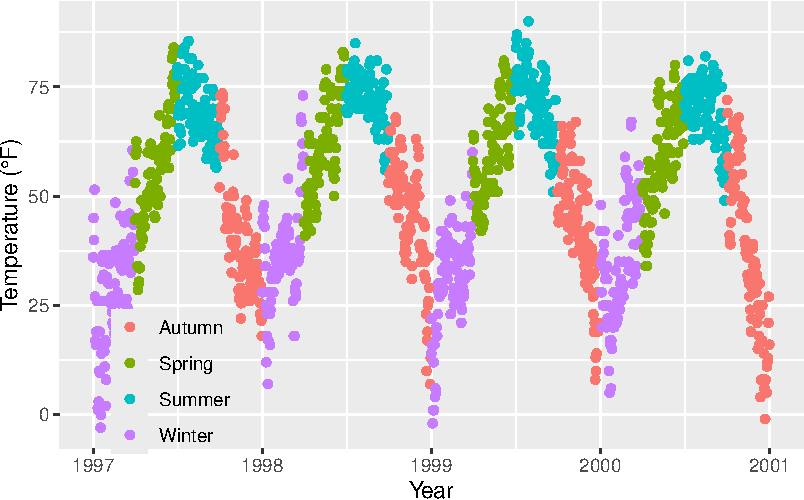
\includegraphics{ch6_files/figure-pdf/legend-inside-1.pdf}

Here, I also override the default white legend background with a
transparent fill to ensure the legend doesn't obscure any data points.

\section{Modifying Legend Direction}\label{modifying-legend-direction}

By default, the legend direction is vertical. However, when you select
either the ``top'' or ``bottom'' position, it becomes horizontal.
Nevertheless, you can freely switch the direction as desired:

\begin{Shaded}
\begin{Highlighting}[]
\FunctionTok{ggplot}\NormalTok{(chic, }\FunctionTok{aes}\NormalTok{(}\AttributeTok{x =}\NormalTok{ date, }\AttributeTok{y =}\NormalTok{ temp, }\AttributeTok{color =}\NormalTok{ season)) }\SpecialCharTok{+}
  \FunctionTok{geom\_point}\NormalTok{() }\SpecialCharTok{+}
  \FunctionTok{labs}\NormalTok{(}\AttributeTok{x =} \StringTok{"Year"}\NormalTok{, }\AttributeTok{y =} \StringTok{"Temperature (°F)"}\NormalTok{) }\SpecialCharTok{+}
  \FunctionTok{theme}\NormalTok{(}\AttributeTok{legend.position =} \FunctionTok{c}\NormalTok{(.}\DecValTok{5}\NormalTok{, .}\DecValTok{97}\NormalTok{),}
        \AttributeTok{legend.background =} \FunctionTok{element\_rect}\NormalTok{(}\AttributeTok{fill =} \StringTok{"transparent"}\NormalTok{)) }\SpecialCharTok{+}
  \FunctionTok{guides}\NormalTok{(}\AttributeTok{color =} \FunctionTok{guide\_legend}\NormalTok{(}\AttributeTok{direction =} \StringTok{"horizontal"}\NormalTok{))}
\end{Highlighting}
\end{Shaded}

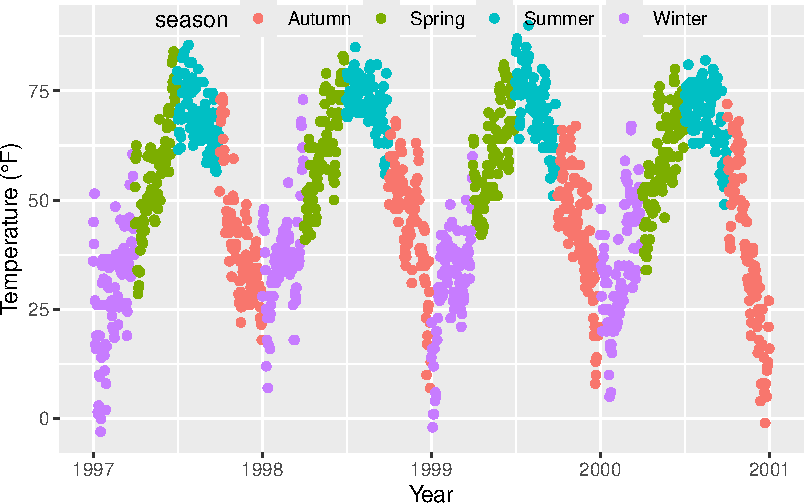
\includegraphics{ch6_files/figure-pdf/legend-orientation-1.pdf}

\section{Change Style of the Legend
Title}\label{change-style-of-the-legend-title}

You can customize the appearance of the legend title by adjusting the
theme element \texttt{legend.title}:

\begin{Shaded}
\begin{Highlighting}[]
\FunctionTok{ggplot}\NormalTok{(chic, }\FunctionTok{aes}\NormalTok{(}\AttributeTok{x =}\NormalTok{ date, }\AttributeTok{y =}\NormalTok{ temp, }\AttributeTok{color =}\NormalTok{ season)) }\SpecialCharTok{+}
  \FunctionTok{geom\_point}\NormalTok{() }\SpecialCharTok{+}
  \FunctionTok{labs}\NormalTok{(}\AttributeTok{x =} \StringTok{"Year"}\NormalTok{, }\AttributeTok{y =} \StringTok{"Temperature (°F)"}\NormalTok{) }\SpecialCharTok{+}
  \FunctionTok{theme}\NormalTok{(}\AttributeTok{legend.title =} \FunctionTok{element\_text}\NormalTok{(}\AttributeTok{family =} \StringTok{"Playfair Display"}\NormalTok{,}
                                    \AttributeTok{color =} \StringTok{"chocolate"}\NormalTok{,}
                                    \AttributeTok{size =} \DecValTok{14}\NormalTok{, }\AttributeTok{face =} \StringTok{"bold"}\NormalTok{))}
\end{Highlighting}
\end{Shaded}

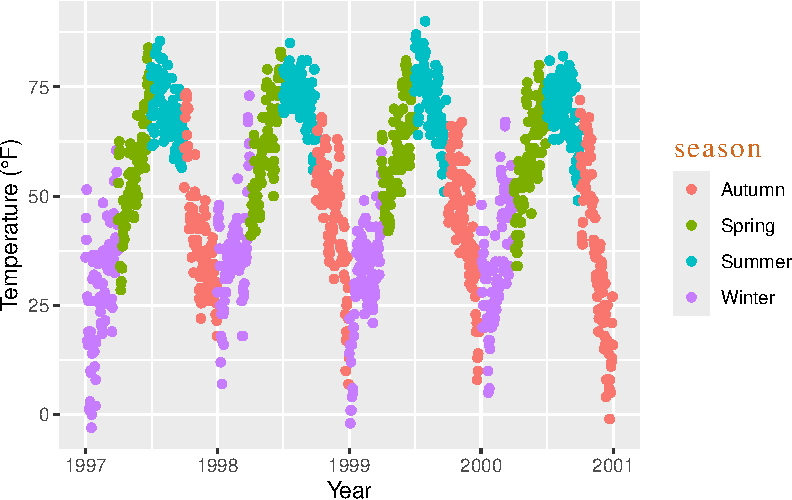
\includegraphics{ch6_files/figure-pdf/legend-style-1.pdf}

\section{Modifying Legend Title}\label{modifying-legend-title}

The simplest method to change the title of the legend is through the
\texttt{labs()} layer:

\begin{Shaded}
\begin{Highlighting}[]
\FunctionTok{ggplot}\NormalTok{(chic, }\FunctionTok{aes}\NormalTok{(}\AttributeTok{x =}\NormalTok{ date, }\AttributeTok{y =}\NormalTok{ temp, }\AttributeTok{color =}\NormalTok{ season)) }\SpecialCharTok{+}
  \FunctionTok{geom\_point}\NormalTok{() }\SpecialCharTok{+}
  \FunctionTok{labs}\NormalTok{(}\AttributeTok{x =} \StringTok{"Year"}\NormalTok{, }\AttributeTok{y =} \StringTok{"Temperature (°F)"}\NormalTok{,}
       \AttributeTok{color =} \StringTok{"Seasons}\SpecialCharTok{\textbackslash{}n}\StringTok{indicated}\SpecialCharTok{\textbackslash{}n}\StringTok{by colors:"}\NormalTok{) }\SpecialCharTok{+}
  \FunctionTok{theme}\NormalTok{(}\AttributeTok{legend.title =} \FunctionTok{element\_text}\NormalTok{(}\AttributeTok{family =} \StringTok{"Playfair Display"}\NormalTok{,}
                                    \AttributeTok{color =} \StringTok{"chocolate"}\NormalTok{,}
                                    \AttributeTok{size =} \DecValTok{14}\NormalTok{, }\AttributeTok{face =} \StringTok{"bold"}\NormalTok{))}
\end{Highlighting}
\end{Shaded}

\includegraphics{ch6_files/figure-pdf/legend-title-labs-1.pdf}

You can adjust the legend details using
\texttt{scale\_color\_discrete(name\ =\ "title")} or
\texttt{guides(color\ =\ guide\_legend("title"))}:

\begin{Shaded}
\begin{Highlighting}[]
\FunctionTok{ggplot}\NormalTok{(chic, }\FunctionTok{aes}\NormalTok{(}\AttributeTok{x =}\NormalTok{ date, }\AttributeTok{y =}\NormalTok{ temp, }\AttributeTok{color =}\NormalTok{ season)) }\SpecialCharTok{+}
  \FunctionTok{geom\_point}\NormalTok{() }\SpecialCharTok{+}
  \FunctionTok{labs}\NormalTok{(}\AttributeTok{x =} \StringTok{"Year"}\NormalTok{, }\AttributeTok{y =} \StringTok{"Temperature (°F)"}\NormalTok{) }\SpecialCharTok{+}
  \FunctionTok{theme}\NormalTok{(}\AttributeTok{legend.title =} \FunctionTok{element\_text}\NormalTok{(}\AttributeTok{family =} \StringTok{"Playfair Display"}\NormalTok{,}
                                    \AttributeTok{color =} \StringTok{"chocolate"}\NormalTok{,}
                                    \AttributeTok{size =} \DecValTok{14}\NormalTok{, }\AttributeTok{face =} \StringTok{"bold"}\NormalTok{)) }\SpecialCharTok{+}
  \FunctionTok{scale\_color\_discrete}\NormalTok{(}\AttributeTok{name =} \StringTok{"Seasons}\SpecialCharTok{\textbackslash{}n}\StringTok{indicated}\SpecialCharTok{\textbackslash{}n}\StringTok{by colors:"}\NormalTok{)}
\end{Highlighting}
\end{Shaded}

\includegraphics{ch6_files/figure-pdf/legend-title-1.pdf}

\section{Rearrange Order of Legend
Keys}\label{rearrange-order-of-legend-keys}

This can be accomplished by changing the levels of \texttt{season}:

\begin{Shaded}
\begin{Highlighting}[]
\NormalTok{chic}\SpecialCharTok{$}\NormalTok{season }\OtherTok{\textless{}{-}}
  \FunctionTok{factor}\NormalTok{(chic}\SpecialCharTok{$}\NormalTok{season,}
         \AttributeTok{levels =} \FunctionTok{c}\NormalTok{(}\StringTok{"Winter"}\NormalTok{, }\StringTok{"Spring"}\NormalTok{, }\StringTok{"Summer"}\NormalTok{, }\StringTok{"Autumn"}\NormalTok{))}

\FunctionTok{ggplot}\NormalTok{(chic, }\FunctionTok{aes}\NormalTok{(}\AttributeTok{x =}\NormalTok{ date, }\AttributeTok{y =}\NormalTok{ temp, }\AttributeTok{color =}\NormalTok{ season)) }\SpecialCharTok{+}
  \FunctionTok{geom\_point}\NormalTok{() }\SpecialCharTok{+}
  \FunctionTok{labs}\NormalTok{(}\AttributeTok{x =} \StringTok{"Year"}\NormalTok{, }\AttributeTok{y =} \StringTok{"Temperature (°F)"}\NormalTok{)}
\end{Highlighting}
\end{Shaded}

\includegraphics{ch6_files/figure-pdf/legend-order-1.pdf}

\section{Modify Legend Labels}\label{modify-legend-labels}

To replace the seasons with the months they represent, provide a vector
of names in the \texttt{scale\_color\_discrete()} call:

\begin{Shaded}
\begin{Highlighting}[]
\FunctionTok{ggplot}\NormalTok{(chic, }\FunctionTok{aes}\NormalTok{(}\AttributeTok{x =}\NormalTok{ date, }\AttributeTok{y =}\NormalTok{ temp, }\AttributeTok{color =}\NormalTok{ season)) }\SpecialCharTok{+}
  \FunctionTok{geom\_point}\NormalTok{() }\SpecialCharTok{+}
  \FunctionTok{labs}\NormalTok{(}\AttributeTok{x =} \StringTok{"Year"}\NormalTok{, }\AttributeTok{y =} \StringTok{"Temperature (°F)"}\NormalTok{) }\SpecialCharTok{+}
  \FunctionTok{scale\_color\_discrete}\NormalTok{(}
    \AttributeTok{name =} \StringTok{"Seasons:"}\NormalTok{,}
    \AttributeTok{labels =} \FunctionTok{c}\NormalTok{(}\StringTok{"Mar—May"}\NormalTok{, }\StringTok{"Jun—Aug"}\NormalTok{, }\StringTok{"Sep—Nov"}\NormalTok{, }\StringTok{"Dec—Feb"}\NormalTok{)}
\NormalTok{  ) }\SpecialCharTok{+}
  \FunctionTok{theme}\NormalTok{(}\AttributeTok{legend.title =} \FunctionTok{element\_text}\NormalTok{(}
    \AttributeTok{family =} \StringTok{"Playfair Display"}\NormalTok{, }\AttributeTok{color =} \StringTok{"chocolate"}\NormalTok{, }\AttributeTok{size =} \DecValTok{14}\NormalTok{, }\AttributeTok{face =} \DecValTok{2}
\NormalTok{  ))}
\end{Highlighting}
\end{Shaded}

\includegraphics{ch6_files/figure-pdf/legend-labels-1.pdf}

\section{Adjust Background Boxes in the
Legend}\label{adjust-background-boxes-in-the-legend}

To alter the background color (fill) of the legend keys, we modify the
setting for the theme element \texttt{legend.key}:

\begin{Shaded}
\begin{Highlighting}[]
\FunctionTok{ggplot}\NormalTok{(chic, }\FunctionTok{aes}\NormalTok{(}\AttributeTok{x =}\NormalTok{ date, }\AttributeTok{y =}\NormalTok{ temp, }\AttributeTok{color =}\NormalTok{ season)) }\SpecialCharTok{+}
  \FunctionTok{geom\_point}\NormalTok{() }\SpecialCharTok{+}
  \FunctionTok{labs}\NormalTok{(}\AttributeTok{x =} \StringTok{"Year"}\NormalTok{, }\AttributeTok{y =} \StringTok{"Temperature (°F)"}\NormalTok{) }\SpecialCharTok{+}
  \FunctionTok{theme}\NormalTok{(}\AttributeTok{legend.key =} \FunctionTok{element\_rect}\NormalTok{(}\AttributeTok{fill =} \StringTok{"darkgoldenrod1"}\NormalTok{),}
        \AttributeTok{legend.title =} \FunctionTok{element\_text}\NormalTok{(}\AttributeTok{family =} \StringTok{"Playfair Display"}\NormalTok{,}
                                    \AttributeTok{color =} \StringTok{"chocolate"}\NormalTok{,}
                                    \AttributeTok{size =} \DecValTok{14}\NormalTok{, }\AttributeTok{face =} \DecValTok{2}\NormalTok{)) }\SpecialCharTok{+}
  \FunctionTok{scale\_color\_discrete}\NormalTok{(}\StringTok{"Seasons:"}\NormalTok{)}
\end{Highlighting}
\end{Shaded}

\includegraphics{ch6_files/figure-pdf/legend-boxes-1.pdf}

If you wish to remove them entirely, use \texttt{fill\ =\ NA} or
\texttt{fill\ =\ "transparent"}.

\section{Adjust Size of Legend
Symbols}\label{adjust-size-of-legend-symbols}

The default size of points in the legend may cause them to appear too
small, especially without boxes. To modify this, you can again use the
\texttt{guides} layer as follows:

\begin{Shaded}
\begin{Highlighting}[]
\FunctionTok{ggplot}\NormalTok{(chic, }\FunctionTok{aes}\NormalTok{(}\AttributeTok{x =}\NormalTok{ date, }\AttributeTok{y =}\NormalTok{ temp, }\AttributeTok{color =}\NormalTok{ season)) }\SpecialCharTok{+}
  \FunctionTok{geom\_point}\NormalTok{() }\SpecialCharTok{+}
  \FunctionTok{labs}\NormalTok{(}\AttributeTok{x =} \StringTok{"Year"}\NormalTok{, }\AttributeTok{y =} \StringTok{"Temperature (°F)"}\NormalTok{) }\SpecialCharTok{+}
  \FunctionTok{theme}\NormalTok{(}\AttributeTok{legend.key =} \FunctionTok{element\_rect}\NormalTok{(}\AttributeTok{fill =} \ConstantTok{NA}\NormalTok{),}
        \AttributeTok{legend.title =} \FunctionTok{element\_text}\NormalTok{(}\AttributeTok{color =} \StringTok{"chocolate"}\NormalTok{,}
                                    \AttributeTok{size =} \DecValTok{14}\NormalTok{, }\AttributeTok{face =} \DecValTok{2}\NormalTok{)) }\SpecialCharTok{+}
  \FunctionTok{scale\_color\_discrete}\NormalTok{(}\StringTok{"Seasons:"}\NormalTok{) }\SpecialCharTok{+}
  \FunctionTok{guides}\NormalTok{(}\AttributeTok{color =} \FunctionTok{guide\_legend}\NormalTok{(}\AttributeTok{override.aes =} \FunctionTok{list}\NormalTok{(}\AttributeTok{size =} \DecValTok{6}\NormalTok{)))}
\end{Highlighting}
\end{Shaded}

\includegraphics{ch6_files/figure-pdf/legend-symbols-1.pdf}

\section{Exclude a Layer from the
Legend}\label{exclude-a-layer-from-the-legend}

Suppose you have two different geometric layers mapped to the same
variable, such as color being used as an aesthetic for both a point
layer and a rug layer of the same data. By default, both the points and
the ``line'' end up in the legend like this:

\begin{Shaded}
\begin{Highlighting}[]
\FunctionTok{ggplot}\NormalTok{(chic, }\FunctionTok{aes}\NormalTok{(}\AttributeTok{x =}\NormalTok{ date, }\AttributeTok{y =}\NormalTok{ temp, }\AttributeTok{color =}\NormalTok{ season)) }\SpecialCharTok{+}
  \FunctionTok{geom\_point}\NormalTok{() }\SpecialCharTok{+}
  \FunctionTok{labs}\NormalTok{(}\AttributeTok{x =} \StringTok{"Year"}\NormalTok{, }\AttributeTok{y =} \StringTok{"Temperature (°F)"}\NormalTok{) }\SpecialCharTok{+}
  \FunctionTok{geom\_rug}\NormalTok{()}
\end{Highlighting}
\end{Shaded}

\includegraphics{ch6_files/figure-pdf/legend-layer-1-1.pdf}

You can utilize \texttt{show.legend\ =\ FALSE} to exclude a layer from
the legend:

\begin{Shaded}
\begin{Highlighting}[]
\FunctionTok{ggplot}\NormalTok{(chic, }\FunctionTok{aes}\NormalTok{(}\AttributeTok{x =}\NormalTok{ date, }\AttributeTok{y =}\NormalTok{ temp, }\AttributeTok{color =}\NormalTok{ season)) }\SpecialCharTok{+}
  \FunctionTok{geom\_point}\NormalTok{() }\SpecialCharTok{+}
  \FunctionTok{labs}\NormalTok{(}\AttributeTok{x =} \StringTok{"Year"}\NormalTok{, }\AttributeTok{y =} \StringTok{"Temperature (°F)"}\NormalTok{) }\SpecialCharTok{+}
  \FunctionTok{geom\_rug}\NormalTok{(}\AttributeTok{show.legend =} \ConstantTok{FALSE}\NormalTok{)}
\end{Highlighting}
\end{Shaded}

\includegraphics{ch6_files/figure-pdf/legend-layer-2-1.pdf}

\section{Manually Adding Legend
Items}\label{manually-adding-legend-items}

By default, \texttt{\{ggplot2\}} won't add a legend unless you map
aesthetics (color, size, etc.) to a variable. However, there are
occasions where you may want to include a legend for clarity.

Here's the default behavior:

\begin{Shaded}
\begin{Highlighting}[]
\FunctionTok{ggplot}\NormalTok{(chic, }\FunctionTok{aes}\NormalTok{(}\AttributeTok{x =}\NormalTok{ date, }\AttributeTok{y =}\NormalTok{ o3)) }\SpecialCharTok{+}
  \FunctionTok{geom\_line}\NormalTok{(}\AttributeTok{color =} \StringTok{"gray"}\NormalTok{) }\SpecialCharTok{+}
  \FunctionTok{geom\_point}\NormalTok{(}\AttributeTok{color =} \StringTok{"darkorange2"}\NormalTok{) }\SpecialCharTok{+}
  \FunctionTok{labs}\NormalTok{(}\AttributeTok{x =} \StringTok{"Year"}\NormalTok{, }\AttributeTok{y =} \StringTok{"Ozone"}\NormalTok{)}
\end{Highlighting}
\end{Shaded}

\includegraphics{ch6_files/figure-pdf/legend-default-2-1.pdf}

To force a legend, we can map a guide to a \emph{variable}. Here, we're
mapping the lines and the points using \texttt{aes()}, but we're not
mapping to a variable in our dataset. Instead, we're using a single
string for each, ensuring we get just one color for each.

\begin{Shaded}
\begin{Highlighting}[]
\FunctionTok{ggplot}\NormalTok{(chic, }\FunctionTok{aes}\NormalTok{(}\AttributeTok{x =}\NormalTok{ date, }\AttributeTok{y =}\NormalTok{ o3)) }\SpecialCharTok{+}
  \FunctionTok{geom\_line}\NormalTok{(}\FunctionTok{aes}\NormalTok{(}\AttributeTok{color =} \StringTok{"line"}\NormalTok{)) }\SpecialCharTok{+}
  \FunctionTok{geom\_point}\NormalTok{(}\FunctionTok{aes}\NormalTok{(}\AttributeTok{color =} \StringTok{"points"}\NormalTok{)) }\SpecialCharTok{+}
  \FunctionTok{labs}\NormalTok{(}\AttributeTok{x =} \StringTok{"Year"}\NormalTok{, }\AttributeTok{y =} \StringTok{"Ozone"}\NormalTok{) }\SpecialCharTok{+}
  \FunctionTok{scale\_color\_discrete}\NormalTok{(}\StringTok{"Type:"}\NormalTok{)}
\end{Highlighting}
\end{Shaded}

\includegraphics{ch6_files/figure-pdf/legend-force-1.pdf}

We're getting close, but this is not what we want. We desire gray lines
and red points. To change the colors, we use
\texttt{scale\_color\_manual()}. Additionally, we override the legend
aesthetics using the \texttt{guide()} function.

Now, we have a plot with gray lines and red points, as well as a single
gray line and a single red point as legend symbols.

\begin{Shaded}
\begin{Highlighting}[]
\FunctionTok{ggplot}\NormalTok{(chic, }\FunctionTok{aes}\NormalTok{(}\AttributeTok{x =}\NormalTok{ date, }\AttributeTok{y =}\NormalTok{ o3)) }\SpecialCharTok{+}
  \FunctionTok{geom\_line}\NormalTok{(}\FunctionTok{aes}\NormalTok{(}\AttributeTok{color =} \StringTok{"line"}\NormalTok{)) }\SpecialCharTok{+}
  \FunctionTok{geom\_point}\NormalTok{(}\FunctionTok{aes}\NormalTok{(}\AttributeTok{color =} \StringTok{"points"}\NormalTok{)) }\SpecialCharTok{+}
  \FunctionTok{labs}\NormalTok{(}\AttributeTok{x =} \StringTok{"Year"}\NormalTok{, }\AttributeTok{y =} \StringTok{"Ozone"}\NormalTok{) }\SpecialCharTok{+}
  \FunctionTok{scale\_color\_manual}\NormalTok{(}\AttributeTok{name =} \ConstantTok{NULL}\NormalTok{,}
                     \AttributeTok{guide =} \StringTok{"legend"}\NormalTok{,}
                     \AttributeTok{values =} \FunctionTok{c}\NormalTok{(}\StringTok{"points"} \OtherTok{=} \StringTok{"darkorange2"}\NormalTok{,}
                                \StringTok{"line"} \OtherTok{=} \StringTok{"gray"}\NormalTok{)) }\SpecialCharTok{+}
  \FunctionTok{guides}\NormalTok{(}\AttributeTok{color =} \FunctionTok{guide\_legend}\NormalTok{(}\AttributeTok{override.aes =} \FunctionTok{list}\NormalTok{(}\AttributeTok{linetype =} \FunctionTok{c}\NormalTok{(}\DecValTok{1}\NormalTok{, }\DecValTok{0}\NormalTok{),}
                                                  \AttributeTok{shape =} \FunctionTok{c}\NormalTok{(}\ConstantTok{NA}\NormalTok{, }\DecValTok{16}\NormalTok{))))}
\end{Highlighting}
\end{Shaded}

\includegraphics{ch6_files/figure-pdf/legend-manual-1.pdf}

\section{Use Other Legend Styles}\label{use-other-legend-styles}

The default legend for categorical variables such as \texttt{season} is
a \texttt{guide\_legend()}, as you have seen in several previous
examples. However, if you map a continuous variable to an aesthetic,
\texttt{\{ggplot2\}} will by default not use \texttt{guide\_legend()}
but \texttt{guide\_colorbar()} (or \texttt{guide\_colourbar()}).

\begin{Shaded}
\begin{Highlighting}[]
\FunctionTok{ggplot}\NormalTok{(chic,}
       \FunctionTok{aes}\NormalTok{(}\AttributeTok{x =}\NormalTok{ date, }\AttributeTok{y =}\NormalTok{ temp, }\AttributeTok{color =}\NormalTok{ temp)) }\SpecialCharTok{+}
  \FunctionTok{geom\_point}\NormalTok{() }\SpecialCharTok{+}
  \FunctionTok{labs}\NormalTok{(}\AttributeTok{x =} \StringTok{"Year"}\NormalTok{, }\AttributeTok{y =} \StringTok{"Temperature (°F)"}\NormalTok{, }\AttributeTok{color =} \StringTok{"Temperature (°F)"}\NormalTok{)}
\end{Highlighting}
\end{Shaded}

\includegraphics{ch6_files/figure-pdf/legend-guide-cont-default-1.pdf}

However, by using \texttt{guide\_legend()}, you can force the legend to
display discrete colors for a given number of breaks as in the case of a
categorical variable:

\begin{Shaded}
\begin{Highlighting}[]
\FunctionTok{ggplot}\NormalTok{(chic,}
       \FunctionTok{aes}\NormalTok{(}\AttributeTok{x =}\NormalTok{ date, }\AttributeTok{y =}\NormalTok{ temp, }\AttributeTok{color =}\NormalTok{ temp)) }\SpecialCharTok{+}
  \FunctionTok{geom\_point}\NormalTok{() }\SpecialCharTok{+}
  \FunctionTok{labs}\NormalTok{(}\AttributeTok{x =} \StringTok{"Year"}\NormalTok{, }\AttributeTok{y =} \StringTok{"Temperature (°F)"}\NormalTok{, }\AttributeTok{color =} \StringTok{"Temperature (°F)"}\NormalTok{) }\SpecialCharTok{+}
  \FunctionTok{guides}\NormalTok{(}\AttributeTok{color =} \FunctionTok{guide\_legend}\NormalTok{())}
\end{Highlighting}
\end{Shaded}

\includegraphics{ch6_files/figure-pdf/legend-guide-cont-legend-1.pdf}

You can also utilize \emph{\emph{binned scales}}:

\begin{Shaded}
\begin{Highlighting}[]
\FunctionTok{ggplot}\NormalTok{(chic,}
       \FunctionTok{aes}\NormalTok{(}\AttributeTok{x =}\NormalTok{ date, }\AttributeTok{y =}\NormalTok{ temp, }\AttributeTok{color =}\NormalTok{ temp)) }\SpecialCharTok{+}
  \FunctionTok{geom\_point}\NormalTok{() }\SpecialCharTok{+}
  \FunctionTok{labs}\NormalTok{(}\AttributeTok{x =} \StringTok{"Year"}\NormalTok{, }\AttributeTok{y =} \StringTok{"Temperature (°F)"}\NormalTok{, }\AttributeTok{color =} \StringTok{"Temperature (°F)"}\NormalTok{) }\SpecialCharTok{+}
  \FunctionTok{guides}\NormalTok{(}\AttributeTok{color =} \FunctionTok{guide\_bins}\NormalTok{())}
\end{Highlighting}
\end{Shaded}

\includegraphics{ch6_files/figure-pdf/legend-guide-cont-bins-1.pdf}

\ldots{} or binned scales as \emph{\emph{discrete colorbars}}:

\begin{Shaded}
\begin{Highlighting}[]
\FunctionTok{ggplot}\NormalTok{(chic,}
       \FunctionTok{aes}\NormalTok{(}\AttributeTok{x =}\NormalTok{ date, }\AttributeTok{y =}\NormalTok{ temp, }\AttributeTok{color =}\NormalTok{ temp)) }\SpecialCharTok{+}
  \FunctionTok{geom\_point}\NormalTok{() }\SpecialCharTok{+}
  \FunctionTok{labs}\NormalTok{(}\AttributeTok{x =} \StringTok{"Year"}\NormalTok{, }\AttributeTok{y =} \StringTok{"Temperature (°F)"}\NormalTok{, }\AttributeTok{color =} \StringTok{"Temperature (°F)"}\NormalTok{) }\SpecialCharTok{+}
  \FunctionTok{guides}\NormalTok{(}\AttributeTok{color =} \FunctionTok{guide\_colorsteps}\NormalTok{())}
\end{Highlighting}
\end{Shaded}

\includegraphics{ch6_files/figure-pdf/legend-guide-cont-steps-1.pdf}

\bookmarksetup{startatroot}

\chapter{Working with Backgrounds \& Grid Lines}\label{style}

To modify the overall appearance of your plot, you can use various
functions. While altering the entire theme of your plot is one option
(covered in detail in the \hyperref[themes]{``Working with Themes''}
section below), you can also make specific changes to individual
elements such as backgrounds and grid lines.

\section{Change the Panel Background
Color}\label{change-the-panel-background-color}

You can adjust the background color (fill) of the panel area (where the
data is plotted) by modifying the theme element
\texttt{panel.background}:

\begin{Shaded}
\begin{Highlighting}[]
\FunctionTok{ggplot}\NormalTok{(chic, }\FunctionTok{aes}\NormalTok{(}\AttributeTok{x =}\NormalTok{ date, }\AttributeTok{y =}\NormalTok{ temp)) }\SpecialCharTok{+}
  \FunctionTok{geom\_point}\NormalTok{(}\AttributeTok{color =} \StringTok{"\#1D8565"}\NormalTok{, }\AttributeTok{size =} \DecValTok{2}\NormalTok{) }\SpecialCharTok{+}
  \FunctionTok{labs}\NormalTok{(}\AttributeTok{x =} \StringTok{"Year"}\NormalTok{, }\AttributeTok{y =} \StringTok{"Temperature (°F)"}\NormalTok{) }\SpecialCharTok{+}
  \FunctionTok{theme}\NormalTok{(}\AttributeTok{panel.background =} \FunctionTok{element\_rect}\NormalTok{(}
    \AttributeTok{fill =} \StringTok{"\#64D2AA"}\NormalTok{, }\AttributeTok{color =} \StringTok{"\#64D2AA"}\NormalTok{, }\AttributeTok{linewidth =} \DecValTok{2}\NormalTok{)}
\NormalTok{  )}
\end{Highlighting}
\end{Shaded}

\includegraphics{ch7_files/figure-pdf/panel-color-1.pdf}

Keep in mind that the true color --- the outline of the panel background
--- didn't change despite our specification. This is because there's a
layer on top of \texttt{panel.background}, namely \texttt{panel.border}.
However, it's important to use a transparent fill here; otherwise, your
data will be hidden behind this layer. In the following example, I
illustrate this by using a semitransparent hex color for the
\texttt{fill} argument in \texttt{element\_rect}:

\begin{Shaded}
\begin{Highlighting}[]
\FunctionTok{ggplot}\NormalTok{(chic, }\FunctionTok{aes}\NormalTok{(}\AttributeTok{x =}\NormalTok{ date, }\AttributeTok{y =}\NormalTok{ temp)) }\SpecialCharTok{+}
  \FunctionTok{geom\_point}\NormalTok{(}\AttributeTok{color =} \StringTok{"\#1D8565"}\NormalTok{, }\AttributeTok{size =} \DecValTok{2}\NormalTok{) }\SpecialCharTok{+}
  \FunctionTok{labs}\NormalTok{(}\AttributeTok{x =} \StringTok{"Year"}\NormalTok{, }\AttributeTok{y =} \StringTok{"Temperature (°F)"}\NormalTok{) }\SpecialCharTok{+}
  \FunctionTok{theme}\NormalTok{(}\AttributeTok{panel.border =} \FunctionTok{element\_rect}\NormalTok{(}
    \AttributeTok{fill =} \StringTok{"\#64D2AA99"}\NormalTok{, }\AttributeTok{color =} \StringTok{"\#64D2AA"}\NormalTok{, }\AttributeTok{linewidth =} \DecValTok{2}\NormalTok{)}
\NormalTok{  )}
\end{Highlighting}
\end{Shaded}

\includegraphics{ch7_files/figure-pdf/panel-color-2-1.pdf}

\section{Change Grid Lines}\label{change-grid-lines}

There are two types of grid lines: major grid lines indicating the ticks
and minor grid lines between the major ones. You can customize both by
overwriting the defaults for \texttt{panel.grid} or for each set of
gridlines separately, \texttt{panel.grid.major} and
\texttt{panel.grid.minor}.

\begin{Shaded}
\begin{Highlighting}[]
\FunctionTok{ggplot}\NormalTok{(chic, }\FunctionTok{aes}\NormalTok{(}\AttributeTok{x =}\NormalTok{ date, }\AttributeTok{y =}\NormalTok{ temp)) }\SpecialCharTok{+}
  \FunctionTok{geom\_point}\NormalTok{(}\AttributeTok{color =} \StringTok{"firebrick"}\NormalTok{) }\SpecialCharTok{+}
  \FunctionTok{labs}\NormalTok{(}\AttributeTok{x =} \StringTok{"Year"}\NormalTok{, }\AttributeTok{y =} \StringTok{"Temperature (°F)"}\NormalTok{) }\SpecialCharTok{+}
  \FunctionTok{theme}\NormalTok{(}\AttributeTok{panel.grid.major =} \FunctionTok{element\_line}\NormalTok{(}\AttributeTok{color =} \StringTok{"gray10"}\NormalTok{, }\AttributeTok{linewidth =}\NormalTok{ .}\DecValTok{5}\NormalTok{),}
        \AttributeTok{panel.grid.minor =} \FunctionTok{element\_line}\NormalTok{(}\AttributeTok{color =} \StringTok{"gray70"}\NormalTok{, }\AttributeTok{linewidth =}\NormalTok{ .}\DecValTok{25}\NormalTok{))}
\end{Highlighting}
\end{Shaded}

\includegraphics{ch7_files/figure-pdf/grid-lines-1.pdf}

You can even specify settings for all four different levels of grid
lines: major horizontal, major vertical, minor horizontal, and minor
vertical.

\begin{Shaded}
\begin{Highlighting}[]
\FunctionTok{ggplot}\NormalTok{(chic, }\FunctionTok{aes}\NormalTok{(}\AttributeTok{x =}\NormalTok{ date, }\AttributeTok{y =}\NormalTok{ temp)) }\SpecialCharTok{+}
  \FunctionTok{geom\_point}\NormalTok{(}\AttributeTok{color =} \StringTok{"firebrick"}\NormalTok{) }\SpecialCharTok{+}
  \FunctionTok{labs}\NormalTok{(}\AttributeTok{x =} \StringTok{"Year"}\NormalTok{, }\AttributeTok{y =} \StringTok{"Temperature (°F)"}\NormalTok{) }\SpecialCharTok{+}
  \FunctionTok{theme}\NormalTok{(}\AttributeTok{panel.grid.major =} \FunctionTok{element\_line}\NormalTok{(}\AttributeTok{linewidth =}\NormalTok{ .}\DecValTok{5}\NormalTok{, }\AttributeTok{linetype =} \StringTok{"dashed"}\NormalTok{),}
        \AttributeTok{panel.grid.minor =} \FunctionTok{element\_line}\NormalTok{(}\AttributeTok{linewidth =}\NormalTok{ .}\DecValTok{25}\NormalTok{, }\AttributeTok{linetype =} \StringTok{"dotted"}\NormalTok{),}
        \AttributeTok{panel.grid.major.x =} \FunctionTok{element\_line}\NormalTok{(}\AttributeTok{color =} \StringTok{"red1"}\NormalTok{),}
        \AttributeTok{panel.grid.major.y =} \FunctionTok{element\_line}\NormalTok{(}\AttributeTok{color =} \StringTok{"blue1"}\NormalTok{),}
        \AttributeTok{panel.grid.minor.x =} \FunctionTok{element\_line}\NormalTok{(}\AttributeTok{color =} \StringTok{"red4"}\NormalTok{),}
        \AttributeTok{panel.grid.minor.y =} \FunctionTok{element\_line}\NormalTok{(}\AttributeTok{color =} \StringTok{"blue4"}\NormalTok{))}
\end{Highlighting}
\end{Shaded}

\includegraphics{ch7_files/figure-pdf/grid-lines-x-y-1.pdf}

And, of course, you can remove some or all grid lines if you like. For
instance, to remove all grid lines, you can set
\texttt{panel.grid\ =\ element\_blank()}. Alternatively, you can remove
only major or minor grid lines by specifying \texttt{panel.grid.major}
or \texttt{panel.grid.minor} accordingly and setting them to
\texttt{element\_blank()}.

\begin{Shaded}
\begin{Highlighting}[]
\FunctionTok{ggplot}\NormalTok{(chic, }\FunctionTok{aes}\NormalTok{(}\AttributeTok{x =}\NormalTok{ date, }\AttributeTok{y =}\NormalTok{ temp)) }\SpecialCharTok{+}
  \FunctionTok{geom\_point}\NormalTok{(}\AttributeTok{color =} \StringTok{"firebrick"}\NormalTok{) }\SpecialCharTok{+}
  \FunctionTok{labs}\NormalTok{(}\AttributeTok{x =} \StringTok{"Year"}\NormalTok{, }\AttributeTok{y =} \StringTok{"Temperature (°F)"}\NormalTok{) }\SpecialCharTok{+}
  \FunctionTok{theme}\NormalTok{(}\AttributeTok{panel.grid.minor =} \FunctionTok{element\_blank}\NormalTok{())}
\end{Highlighting}
\end{Shaded}

\includegraphics{ch7_files/figure-pdf/grid-remove-1.pdf}

\begin{Shaded}
\begin{Highlighting}[]
\FunctionTok{ggplot}\NormalTok{(chic, }\FunctionTok{aes}\NormalTok{(}\AttributeTok{x =}\NormalTok{ date, }\AttributeTok{y =}\NormalTok{ temp)) }\SpecialCharTok{+}
  \FunctionTok{geom\_point}\NormalTok{(}\AttributeTok{color =} \StringTok{"firebrick"}\NormalTok{) }\SpecialCharTok{+}
  \FunctionTok{labs}\NormalTok{(}\AttributeTok{x =} \StringTok{"Year"}\NormalTok{, }\AttributeTok{y =} \StringTok{"Temperature (°F)"}\NormalTok{) }\SpecialCharTok{+}
  \FunctionTok{theme}\NormalTok{(}\AttributeTok{panel.grid =} \FunctionTok{element\_blank}\NormalTok{())}
\end{Highlighting}
\end{Shaded}

\includegraphics{ch7_files/figure-pdf/grid-blank-1.pdf}

\section{Change Spacing of Gridlines}\label{change-spacing-of-gridlines}

Furthermore, you can also define the breaks between both major and minor
grid lines by specifying the \texttt{breaks} argument.

\begin{Shaded}
\begin{Highlighting}[]
\FunctionTok{ggplot}\NormalTok{(chic, }\FunctionTok{aes}\NormalTok{(}\AttributeTok{x =}\NormalTok{ date, }\AttributeTok{y =}\NormalTok{ temp)) }\SpecialCharTok{+}
  \FunctionTok{geom\_point}\NormalTok{(}\AttributeTok{color =} \StringTok{"firebrick"}\NormalTok{) }\SpecialCharTok{+}
  \FunctionTok{labs}\NormalTok{(}\AttributeTok{x =} \StringTok{"Year"}\NormalTok{, }\AttributeTok{y =} \StringTok{"Temperature (°F)"}\NormalTok{) }\SpecialCharTok{+}
  \FunctionTok{scale\_y\_continuous}\NormalTok{(}\AttributeTok{breaks =} \FunctionTok{seq}\NormalTok{(}\DecValTok{0}\NormalTok{, }\DecValTok{100}\NormalTok{, }\DecValTok{10}\NormalTok{),}
                     \AttributeTok{minor\_breaks =} \FunctionTok{seq}\NormalTok{(}\DecValTok{0}\NormalTok{, }\DecValTok{100}\NormalTok{, }\FloatTok{2.5}\NormalTok{))}
\end{Highlighting}
\end{Shaded}

\includegraphics{ch7_files/figure-pdf/grid-breaks-1.pdf}

\section{Change the Plot Background
Color}\label{change-the-plot-background-color}

Similarly, to change the background color (fill) of the plot area, you
can modify the theme element \texttt{plot.background} using the
\texttt{theme()} function. This allows you to customize the appearance
of the entire plot area according to your preferences.

\begin{Shaded}
\begin{Highlighting}[]
\FunctionTok{ggplot}\NormalTok{(chic, }\FunctionTok{aes}\NormalTok{(}\AttributeTok{x =}\NormalTok{ date, }\AttributeTok{y =}\NormalTok{ temp)) }\SpecialCharTok{+}
  \FunctionTok{geom\_point}\NormalTok{(}\AttributeTok{color =} \StringTok{"firebrick"}\NormalTok{) }\SpecialCharTok{+}
  \FunctionTok{labs}\NormalTok{(}\AttributeTok{x =} \StringTok{"Year"}\NormalTok{, }\AttributeTok{y =} \StringTok{"Temperature (°F)"}\NormalTok{) }\SpecialCharTok{+}
  \FunctionTok{theme}\NormalTok{(}\AttributeTok{plot.background =} \FunctionTok{element\_rect}\NormalTok{(}\AttributeTok{fill =} \StringTok{"gray60"}\NormalTok{,}
                                       \AttributeTok{color =} \StringTok{"gray30"}\NormalTok{, }\AttributeTok{linewidth =} \DecValTok{2}\NormalTok{))}
\end{Highlighting}
\end{Shaded}

\includegraphics{ch7_files/figure-pdf/background-color-1.pdf}

You can achieve a unique background color by either setting the same
colors in both \texttt{panel.background} and \texttt{plot.background} or
by setting the background filling of the panel to \texttt{"transparent"}
or \texttt{NA}. This customization can help you create visually
appealing plots that match your design preferences.

\begin{Shaded}
\begin{Highlighting}[]
\FunctionTok{ggplot}\NormalTok{(chic, }\FunctionTok{aes}\NormalTok{(}\AttributeTok{x =}\NormalTok{ date, }\AttributeTok{y =}\NormalTok{ temp)) }\SpecialCharTok{+}
  \FunctionTok{geom\_point}\NormalTok{(}\AttributeTok{color =} \StringTok{"firebrick"}\NormalTok{) }\SpecialCharTok{+}
  \FunctionTok{labs}\NormalTok{(}\AttributeTok{x =} \StringTok{"Year"}\NormalTok{, }\AttributeTok{y =} \StringTok{"Temperature (°F)"}\NormalTok{) }\SpecialCharTok{+}
  \FunctionTok{theme}\NormalTok{(}\AttributeTok{panel.background =} \FunctionTok{element\_rect}\NormalTok{(}\AttributeTok{fill =} \ConstantTok{NA}\NormalTok{),}
        \AttributeTok{plot.background =} \FunctionTok{element\_rect}\NormalTok{(}\AttributeTok{fill =} \StringTok{"gray60"}\NormalTok{,}
                                       \AttributeTok{color =} \StringTok{"gray30"}\NormalTok{, }\AttributeTok{linewidth =} \DecValTok{2}\NormalTok{))}
\end{Highlighting}
\end{Shaded}

\includegraphics{ch7_files/figure-pdf/background-color-same-1.pdf}

\bookmarksetup{startatroot}

\chapter{Working with Margins}\label{margins}

Sometimes it is useful to add a little space to the plot margin. Similar
to the previous examples, we can use an argument to the \texttt{theme()}
function. In this case, the argument is \texttt{plot.margin}. As
illustrated in the previous example where we changed the background
color using \texttt{plot.background}, we can now add extra space to both
the left and right.

The \texttt{plot.margin} argument can handle a variety of different
units (cm, inches, etc.), but it requires the use of the \texttt{unit}
function from the package \texttt{grid} to specify the units. You can
either provide the same value for all sides (easiest via
\texttt{rep(x,\ 4)}) or particular distances for each. Here, I am using
a 1cm margin on the top and bottom, 3 cm margin on the right, and an 8
cm margin on the left.

\begin{Shaded}
\begin{Highlighting}[]
\FunctionTok{ggplot}\NormalTok{(chic, }\FunctionTok{aes}\NormalTok{(}\AttributeTok{x =}\NormalTok{ date, }\AttributeTok{y =}\NormalTok{ temp)) }\SpecialCharTok{+}
  \FunctionTok{geom\_point}\NormalTok{(}\AttributeTok{color =} \StringTok{"firebrick"}\NormalTok{) }\SpecialCharTok{+}
  \FunctionTok{labs}\NormalTok{(}\AttributeTok{x =} \StringTok{"Year"}\NormalTok{, }\AttributeTok{y =} \StringTok{"Temperature (°F)"}\NormalTok{) }\SpecialCharTok{+}
  \FunctionTok{theme}\NormalTok{(}\AttributeTok{plot.background =} \FunctionTok{element\_rect}\NormalTok{(}\AttributeTok{fill =} \StringTok{"gray60"}\NormalTok{),}
        \AttributeTok{plot.margin =} \FunctionTok{margin}\NormalTok{(}\AttributeTok{t =} \DecValTok{1}\NormalTok{, }\AttributeTok{r =} \DecValTok{3}\NormalTok{, }\AttributeTok{b =} \DecValTok{1}\NormalTok{, }\AttributeTok{l =} \DecValTok{8}\NormalTok{, }\AttributeTok{unit =} \StringTok{"cm"}\NormalTok{))}
\end{Highlighting}
\end{Shaded}

\includegraphics{ch8_files/figure-pdf/margin-1.pdf}

💁 You can also use \texttt{unit()} instead of \texttt{margin()}. Expand
to see example.

\begin{Shaded}
\begin{Highlighting}[]
\FunctionTok{ggplot}\NormalTok{(chic, }\FunctionTok{aes}\NormalTok{(}\AttributeTok{x =}\NormalTok{ date, }\AttributeTok{y =}\NormalTok{ temp)) }\SpecialCharTok{+}
  \FunctionTok{geom\_point}\NormalTok{(}\AttributeTok{color =} \StringTok{"firebrick"}\NormalTok{) }\SpecialCharTok{+}
  \FunctionTok{labs}\NormalTok{(}\AttributeTok{x =} \StringTok{"Year"}\NormalTok{, }\AttributeTok{y =} \StringTok{"Temperature (°F)"}\NormalTok{) }\SpecialCharTok{+}
  \FunctionTok{theme}\NormalTok{(}\AttributeTok{plot.background =} \FunctionTok{element\_rect}\NormalTok{(}\AttributeTok{fill =} \StringTok{"gray60"}\NormalTok{),}
        \AttributeTok{plot.margin =} \FunctionTok{unit}\NormalTok{(}\FunctionTok{c}\NormalTok{(}\DecValTok{1}\NormalTok{, }\DecValTok{3}\NormalTok{, }\DecValTok{1}\NormalTok{, }\DecValTok{8}\NormalTok{), }\StringTok{"cm"}\NormalTok{))}
\end{Highlighting}
\end{Shaded}

\includegraphics{ch8_files/figure-pdf/margin-2-1.pdf}

\bookmarksetup{startatroot}

\chapter{Working with Multi-Panel Plots}\label{panels}

The \texttt{\{ggplot2\}} package offers two handy functions for creating
multi-panel plots, called \emph{facets}. They are related but have
slight differences: \texttt{facet\_wrap} creates a ribbon of plots based
on a single variable, while \texttt{facet\_grid} spans a grid of plots
based on two variables.

\section{Create a Grid of Small Multiples Based on Two
Variables}\label{create-a-grid-of-small-multiples-based-on-two-variables}

When dealing with two variables, \texttt{facet\_grid} is the appropriate
choice. In this function, the order of the variables determines the
number of rows and columns in the grid:

\begin{Shaded}
\begin{Highlighting}[]
\FunctionTok{ggplot}\NormalTok{(chic, }\FunctionTok{aes}\NormalTok{(}\AttributeTok{x =}\NormalTok{ date, }\AttributeTok{y =}\NormalTok{ temp)) }\SpecialCharTok{+}
  \FunctionTok{geom\_point}\NormalTok{(}\AttributeTok{color =} \StringTok{"orangered"}\NormalTok{, }\AttributeTok{alpha =}\NormalTok{ .}\DecValTok{3}\NormalTok{) }\SpecialCharTok{+}
  \FunctionTok{theme}\NormalTok{(}\AttributeTok{axis.text.x =} \FunctionTok{element\_text}\NormalTok{(}\AttributeTok{angle =} \DecValTok{45}\NormalTok{, }\AttributeTok{vjust =} \DecValTok{1}\NormalTok{, }\AttributeTok{hjust =} \DecValTok{1}\NormalTok{)) }\SpecialCharTok{+}
  \FunctionTok{labs}\NormalTok{(}\AttributeTok{x =} \StringTok{"Year"}\NormalTok{, }\AttributeTok{y =} \StringTok{"Temperature (°F)"}\NormalTok{) }\SpecialCharTok{+}
  \FunctionTok{facet\_grid}\NormalTok{(year }\SpecialCharTok{\textasciitilde{}}\NormalTok{ season)}
\end{Highlighting}
\end{Shaded}

\includegraphics{ch9_files/figure-pdf/grid-plots-1.pdf}

To switch from a row-based arrangement to a column-based one, you can
modify \texttt{facet\_grid(year\ \textasciitilde{}\ season)} to
\texttt{facet\_grid(season\ \textasciitilde{}\ year)}.

\section{Create Small Multiples Based on One
Variable}\label{create-small-multiples-based-on-one-variable}

\texttt{facet\_wrap} creates a facet of a single variable, specified
with a tilde in front:
\texttt{facet\_wrap(\textasciitilde{}\ variable)}. The appearance of
these subplots is determined by the arguments \texttt{ncol} and
\texttt{nrow}:

\begin{Shaded}
\begin{Highlighting}[]
\NormalTok{g }\OtherTok{\textless{}{-}}
  \FunctionTok{ggplot}\NormalTok{(chic, }\FunctionTok{aes}\NormalTok{(}\AttributeTok{x =}\NormalTok{ date, }\AttributeTok{y =}\NormalTok{ temp)) }\SpecialCharTok{+}
    \FunctionTok{geom\_point}\NormalTok{(}\AttributeTok{color =} \StringTok{"chartreuse4"}\NormalTok{, }\AttributeTok{alpha =}\NormalTok{ .}\DecValTok{3}\NormalTok{) }\SpecialCharTok{+}
    \FunctionTok{labs}\NormalTok{(}\AttributeTok{x =} \StringTok{"Year"}\NormalTok{, }\AttributeTok{y =} \StringTok{"Temperature (°F)"}\NormalTok{) }\SpecialCharTok{+}
    \FunctionTok{theme}\NormalTok{(}\AttributeTok{axis.text.x =} \FunctionTok{element\_text}\NormalTok{(}\AttributeTok{angle =} \DecValTok{45}\NormalTok{, }\AttributeTok{vjust =} \DecValTok{1}\NormalTok{, }\AttributeTok{hjust =} \DecValTok{1}\NormalTok{))}

\NormalTok{g }\SpecialCharTok{+} \FunctionTok{facet\_wrap}\NormalTok{(}\SpecialCharTok{\textasciitilde{}}\NormalTok{ year)}
\end{Highlighting}
\end{Shaded}

\includegraphics{ch9_files/figure-pdf/wrap-plots-1-row-1.pdf}

Accordingly, you can arrange the plots as you like, instead as a matrix
in one row\ldots{}

\begin{Shaded}
\begin{Highlighting}[]
\NormalTok{g }\SpecialCharTok{+} \FunctionTok{facet\_wrap}\NormalTok{(}\SpecialCharTok{\textasciitilde{}}\NormalTok{ year, }\AttributeTok{nrow =} \DecValTok{1}\NormalTok{)}
\end{Highlighting}
\end{Shaded}

\includegraphics{ch9_files/figure-pdf/wrap-plots-2-rows-1.pdf}

\ldots{} or even as a asymmetric grid of plots:

\begin{Shaded}
\begin{Highlighting}[]
\NormalTok{g }\SpecialCharTok{+} \FunctionTok{facet\_wrap}\NormalTok{(}\SpecialCharTok{\textasciitilde{}}\NormalTok{ year, }\AttributeTok{ncol =} \DecValTok{3}\NormalTok{) }\SpecialCharTok{+} \FunctionTok{theme}\NormalTok{(}\AttributeTok{axis.title.x =} \FunctionTok{element\_text}\NormalTok{(}\AttributeTok{hjust =}\NormalTok{ .}\DecValTok{15}\NormalTok{))}
\end{Highlighting}
\end{Shaded}

\includegraphics{ch9_files/figure-pdf/wrap-plots-2-rows-3-col-1.pdf}

\section{Allow Axes to Roam Free}\label{allow-axes-to-roam-free}

The default for multi-panel plots in \texttt{\{ggplot2\}} is to use
equivalent scales in each panel. But sometimes you want to allow a
panels own data to determine the scale. This is often not a good idea
since it may give your user the wrong impression about the data. But
sometimes it is indeed useful and to do this you can set
\texttt{scales\ =\ "free"}:

\begin{Shaded}
\begin{Highlighting}[]
\NormalTok{g }\SpecialCharTok{+} \FunctionTok{facet\_wrap}\NormalTok{(}\SpecialCharTok{\textasciitilde{}}\NormalTok{ year, }\AttributeTok{nrow =} \DecValTok{2}\NormalTok{, }\AttributeTok{scales =} \StringTok{"free"}\NormalTok{)}
\end{Highlighting}
\end{Shaded}

\includegraphics{ch9_files/figure-pdf/wrap-plots-scales-free-1.pdf}

Note that both, x and y axes differ in their range!

\subsubsection{\texorpdfstring{Use \texttt{facet\_wrap} with Two
Variables}{Use facet\_wrap with Two Variables}}\label{use-facet_wrap-with-two-variables}

The function \texttt{facet\_wrap} can also take two variables:

\begin{Shaded}
\begin{Highlighting}[]
\NormalTok{g }\SpecialCharTok{+} \FunctionTok{facet\_wrap}\NormalTok{(year }\SpecialCharTok{\textasciitilde{}}\NormalTok{ season, }\AttributeTok{nrow =} \DecValTok{4}\NormalTok{, }\AttributeTok{scales =} \StringTok{"free\_x"}\NormalTok{)}
\end{Highlighting}
\end{Shaded}

\includegraphics{ch9_files/figure-pdf/wrap-plots-two-vars-1.pdf}

When using \texttt{facet\_wrap} you are still able to control the grid
design: you can rearrange the number of plots per row and column and you
can also let all axes roam free. In contrast, \texttt{facet\_grid} will
also take a \texttt{free} argument but will only let it roam free per
column or row:

\begin{Shaded}
\begin{Highlighting}[]
\NormalTok{g }\SpecialCharTok{+} \FunctionTok{facet\_grid}\NormalTok{(year }\SpecialCharTok{\textasciitilde{}}\NormalTok{ season, }\AttributeTok{scales =} \StringTok{"free\_x"}\NormalTok{)}
\end{Highlighting}
\end{Shaded}

\includegraphics{ch9_files/figure-pdf/grid-plots-two-vars-1.pdf}

\section{Modify Style of Strip Texts}\label{modify-style-of-strip-texts}

By using \texttt{theme}, you can modify the appearance of the strip text
(i.e.~the title for each facet) and the strip text boxes:

\begin{Shaded}
\begin{Highlighting}[]
\NormalTok{g }\SpecialCharTok{+} \FunctionTok{facet\_wrap}\NormalTok{(}\SpecialCharTok{\textasciitilde{}}\NormalTok{ year, }\AttributeTok{nrow =} \DecValTok{1}\NormalTok{, }\AttributeTok{scales =} \StringTok{"free\_x"}\NormalTok{) }\SpecialCharTok{+}
  \FunctionTok{theme}\NormalTok{(}\AttributeTok{strip.text =} \FunctionTok{element\_text}\NormalTok{(}\AttributeTok{face =} \StringTok{"bold"}\NormalTok{, }\AttributeTok{color =} \StringTok{"chartreuse4"}\NormalTok{,}
                                  \AttributeTok{hjust =} \DecValTok{0}\NormalTok{, }\AttributeTok{size =} \DecValTok{20}\NormalTok{),}
        \AttributeTok{strip.background =} \FunctionTok{element\_rect}\NormalTok{(}\AttributeTok{fill =} \StringTok{"chartreuse3"}\NormalTok{, }\AttributeTok{linetype =} \StringTok{"dotted"}\NormalTok{))}
\end{Highlighting}
\end{Shaded}

\includegraphics{ch9_files/figure-pdf/facet-modify-striptext-1.pdf}

The following
\href{https://stackoverflow.com/questions/60332202/conditionally-fill-ggtext-text-boxes-in-facet-wrap}{two
functions adapted from this answer by Claus Wilke}, the author of the
\href{https://wilkelab.org/ggtext/}{\texttt{\{ggtext\}} package}, allow
to highlight specific labels in combination with
\texttt{element\_textbox()} that is provided by \texttt{\{ggtext\}}.

\begin{Shaded}
\begin{Highlighting}[]
\FunctionTok{library}\NormalTok{(ggtext)}
\FunctionTok{library}\NormalTok{(purrr) }\DocumentationTok{\#\# for \%||\%}

\NormalTok{element\_textbox\_highlight }\OtherTok{\textless{}{-}} \ControlFlowTok{function}\NormalTok{(..., }\AttributeTok{hi.labels =} \ConstantTok{NULL}\NormalTok{, }\AttributeTok{hi.fill =} \ConstantTok{NULL}\NormalTok{,}
                                      \AttributeTok{hi.col =} \ConstantTok{NULL}\NormalTok{, }\AttributeTok{hi.box.col =} \ConstantTok{NULL}\NormalTok{, }\AttributeTok{hi.family =} \ConstantTok{NULL}\NormalTok{) \{}
  \FunctionTok{structure}\NormalTok{(}
    \FunctionTok{c}\NormalTok{(}\FunctionTok{element\_textbox}\NormalTok{(...),}
      \FunctionTok{list}\NormalTok{(}\AttributeTok{hi.labels =}\NormalTok{ hi.labels, }\AttributeTok{hi.fill =}\NormalTok{ hi.fill, }\AttributeTok{hi.col =}\NormalTok{ hi.col, }\AttributeTok{hi.box.col =}\NormalTok{ hi.box.col, }\AttributeTok{hi.family =}\NormalTok{ hi.family)}
\NormalTok{    ),}
    \AttributeTok{class =} \FunctionTok{c}\NormalTok{(}\StringTok{"element\_textbox\_highlight"}\NormalTok{, }\StringTok{"element\_textbox"}\NormalTok{, }\StringTok{"element\_text"}\NormalTok{, }\StringTok{"element"}\NormalTok{)}
\NormalTok{  )}
\NormalTok{\}}

\NormalTok{element\_grob.element\_textbox\_highlight }\OtherTok{\textless{}{-}} \ControlFlowTok{function}\NormalTok{(element, }\AttributeTok{label =} \StringTok{""}\NormalTok{, ...) \{}
  \ControlFlowTok{if}\NormalTok{ (label }\SpecialCharTok{\%in\%}\NormalTok{ element}\SpecialCharTok{$}\NormalTok{hi.labels) \{}
\NormalTok{    element}\SpecialCharTok{$}\NormalTok{fill }\OtherTok{\textless{}{-}}\NormalTok{ element}\SpecialCharTok{$}\NormalTok{hi.fill }\SpecialCharTok{\%||\%}\NormalTok{ element}\SpecialCharTok{$}\NormalTok{fill}
\NormalTok{    element}\SpecialCharTok{$}\NormalTok{colour }\OtherTok{\textless{}{-}}\NormalTok{ element}\SpecialCharTok{$}\NormalTok{hi.col }\SpecialCharTok{\%||\%}\NormalTok{ element}\SpecialCharTok{$}\NormalTok{colour}
\NormalTok{    element}\SpecialCharTok{$}\NormalTok{box.colour }\OtherTok{\textless{}{-}}\NormalTok{ element}\SpecialCharTok{$}\NormalTok{hi.box.col }\SpecialCharTok{\%||\%}\NormalTok{ element}\SpecialCharTok{$}\NormalTok{box.colour}
\NormalTok{    element}\SpecialCharTok{$}\NormalTok{family }\OtherTok{\textless{}{-}}\NormalTok{ element}\SpecialCharTok{$}\NormalTok{hi.family }\SpecialCharTok{\%||\%}\NormalTok{ element}\SpecialCharTok{$}\NormalTok{family}
\NormalTok{  \}}
  \FunctionTok{NextMethod}\NormalTok{()}
\NormalTok{\}}
\end{Highlighting}
\end{Shaded}

Now you can use it and specify for example all striptexts:

\begin{Shaded}
\begin{Highlighting}[]
\NormalTok{g }\SpecialCharTok{+} \FunctionTok{facet\_wrap}\NormalTok{(year }\SpecialCharTok{\textasciitilde{}}\NormalTok{ season, }\AttributeTok{nrow =} \DecValTok{4}\NormalTok{, }\AttributeTok{scales =} \StringTok{"free\_x"}\NormalTok{) }\SpecialCharTok{+}
  \FunctionTok{theme}\NormalTok{(}
    \AttributeTok{strip.background =} \FunctionTok{element\_blank}\NormalTok{(),}
    \AttributeTok{strip.text =} \FunctionTok{element\_textbox\_highlight}\NormalTok{(}
      \AttributeTok{family =} \StringTok{"Playfair Display"}\NormalTok{, }\AttributeTok{size =} \DecValTok{12}\NormalTok{, }\AttributeTok{face =} \StringTok{"bold"}\NormalTok{,}
      \AttributeTok{fill =} \StringTok{"white"}\NormalTok{, }\AttributeTok{box.color =} \StringTok{"chartreuse4"}\NormalTok{, }\AttributeTok{color =} \StringTok{"chartreuse4"}\NormalTok{,}
      \AttributeTok{halign =}\NormalTok{ .}\DecValTok{5}\NormalTok{, }\AttributeTok{linetype =} \DecValTok{1}\NormalTok{, }\AttributeTok{r =} \FunctionTok{unit}\NormalTok{(}\DecValTok{5}\NormalTok{, }\StringTok{"pt"}\NormalTok{), }\AttributeTok{width =} \FunctionTok{unit}\NormalTok{(}\DecValTok{1}\NormalTok{, }\StringTok{"npc"}\NormalTok{),}
      \AttributeTok{padding =} \FunctionTok{margin}\NormalTok{(}\DecValTok{5}\NormalTok{, }\DecValTok{0}\NormalTok{, }\DecValTok{3}\NormalTok{, }\DecValTok{0}\NormalTok{), }\AttributeTok{margin =} \FunctionTok{margin}\NormalTok{(}\DecValTok{0}\NormalTok{, }\DecValTok{1}\NormalTok{, }\DecValTok{3}\NormalTok{, }\DecValTok{1}\NormalTok{),}
      \AttributeTok{hi.labels =} \FunctionTok{c}\NormalTok{(}\StringTok{"1997"}\NormalTok{, }\StringTok{"1998"}\NormalTok{, }\StringTok{"1999"}\NormalTok{, }\StringTok{"2000"}\NormalTok{),}
      \AttributeTok{hi.fill =} \StringTok{"chartreuse4"}\NormalTok{, }\AttributeTok{hi.box.col =} \StringTok{"black"}\NormalTok{, }\AttributeTok{hi.col =} \StringTok{"white"}
\NormalTok{    )}
\NormalTok{  )}
\end{Highlighting}
\end{Shaded}

\begin{verbatim}
Warning in grid.Call(C_textBounds, as.graphicsAnnot(x$label), x$x, x$y, : font
width unknown for character 0x41

Warning in grid.Call(C_textBounds, as.graphicsAnnot(x$label), x$x, x$y, : font
width unknown for character 0x41
\end{verbatim}

\begin{verbatim}
Warning in grid.Call.graphics(C_text, as.graphicsAnnot(x$label), x$x, x$y, :
font width unknown for character 0x41

Warning in grid.Call.graphics(C_text, as.graphicsAnnot(x$label), x$x, x$y, :
font width unknown for character 0x41

Warning in grid.Call.graphics(C_text, as.graphicsAnnot(x$label), x$x, x$y, :
font width unknown for character 0x41

Warning in grid.Call.graphics(C_text, as.graphicsAnnot(x$label), x$x, x$y, :
font width unknown for character 0x41
\end{verbatim}

\includegraphics{ch9_files/figure-pdf/facet-color-striptext-A-1.pdf}

\begin{Shaded}
\begin{Highlighting}[]
\FunctionTok{ggplot}\NormalTok{(chic, }\FunctionTok{aes}\NormalTok{(}\AttributeTok{x =}\NormalTok{ date, }\AttributeTok{y =}\NormalTok{ temp)) }\SpecialCharTok{+}
  \FunctionTok{geom\_point}\NormalTok{(}\FunctionTok{aes}\NormalTok{(}\AttributeTok{color =}\NormalTok{ season }\SpecialCharTok{==} \StringTok{"Summer"}\NormalTok{), }\AttributeTok{alpha =}\NormalTok{ .}\DecValTok{3}\NormalTok{) }\SpecialCharTok{+}
  \FunctionTok{labs}\NormalTok{(}\AttributeTok{x =} \StringTok{"Year"}\NormalTok{, }\AttributeTok{y =} \StringTok{"Temperature (°F)"}\NormalTok{) }\SpecialCharTok{+}
  \FunctionTok{facet\_wrap}\NormalTok{(}\SpecialCharTok{\textasciitilde{}}\NormalTok{ season, }\AttributeTok{nrow =} \DecValTok{1}\NormalTok{) }\SpecialCharTok{+}
  \FunctionTok{scale\_color\_manual}\NormalTok{(}\AttributeTok{values =} \FunctionTok{c}\NormalTok{(}\StringTok{"gray40"}\NormalTok{, }\StringTok{"firebrick"}\NormalTok{), }\AttributeTok{guide =} \StringTok{"none"}\NormalTok{) }\SpecialCharTok{+}
  \FunctionTok{theme}\NormalTok{(}
    \AttributeTok{axis.text.x =} \FunctionTok{element\_text}\NormalTok{(}\AttributeTok{angle =} \DecValTok{45}\NormalTok{, }\AttributeTok{vjust =} \DecValTok{1}\NormalTok{, }\AttributeTok{hjust =} \DecValTok{1}\NormalTok{),}
    \AttributeTok{strip.background =} \FunctionTok{element\_blank}\NormalTok{(),}
    \AttributeTok{strip.text =} \FunctionTok{element\_textbox\_highlight}\NormalTok{(}
      \AttributeTok{size =} \DecValTok{12}\NormalTok{, }\AttributeTok{face =} \StringTok{"bold"}\NormalTok{,}
      \AttributeTok{fill =} \StringTok{"white"}\NormalTok{, }\AttributeTok{box.color =} \StringTok{"white"}\NormalTok{, }\AttributeTok{color =} \StringTok{"gray40"}\NormalTok{,}
      \AttributeTok{halign =}\NormalTok{ .}\DecValTok{5}\NormalTok{, }\AttributeTok{linetype =} \DecValTok{1}\NormalTok{, }\AttributeTok{r =} \FunctionTok{unit}\NormalTok{(}\DecValTok{0}\NormalTok{, }\StringTok{"pt"}\NormalTok{), }\AttributeTok{width =} \FunctionTok{unit}\NormalTok{(}\DecValTok{1}\NormalTok{, }\StringTok{"npc"}\NormalTok{),}
      \AttributeTok{padding =} \FunctionTok{margin}\NormalTok{(}\DecValTok{2}\NormalTok{, }\DecValTok{0}\NormalTok{, }\DecValTok{1}\NormalTok{, }\DecValTok{0}\NormalTok{), }\AttributeTok{margin =} \FunctionTok{margin}\NormalTok{(}\DecValTok{0}\NormalTok{, }\DecValTok{1}\NormalTok{, }\DecValTok{3}\NormalTok{, }\DecValTok{1}\NormalTok{),}
      \AttributeTok{hi.labels =} \StringTok{"Summer"}\NormalTok{, }\AttributeTok{hi.family =} \StringTok{"Bangers"}\NormalTok{,}
      \AttributeTok{hi.fill =} \StringTok{"firebrick"}\NormalTok{, }\AttributeTok{hi.box.col =} \StringTok{"firebrick"}\NormalTok{, }\AttributeTok{hi.col =} \StringTok{"white"}
\NormalTok{    )}
\NormalTok{  )}
\end{Highlighting}
\end{Shaded}

\includegraphics{ch9_files/figure-pdf/r-facet-color-striptext-B-1.pdf}

\section{Create a Panel of Different
Plots}\label{create-a-panel-of-different-plots}

There are several ways how plots can be combined. The easiest approach
in my opinion is the
\href{https://github.com/thomasp85/patchwork}{\texttt{\{patchwork\}}
package} by Thomas Lin Pedersen:

\begin{Shaded}
\begin{Highlighting}[]
\NormalTok{p1 }\OtherTok{\textless{}{-}} \FunctionTok{ggplot}\NormalTok{(chic, }\FunctionTok{aes}\NormalTok{(}\AttributeTok{x =}\NormalTok{ date, }\AttributeTok{y =}\NormalTok{ temp,}
                       \AttributeTok{color =}\NormalTok{ season)) }\SpecialCharTok{+}
        \FunctionTok{geom\_point}\NormalTok{() }\SpecialCharTok{+}
        \FunctionTok{geom\_rug}\NormalTok{() }\SpecialCharTok{+}
        \FunctionTok{labs}\NormalTok{(}\AttributeTok{x =} \StringTok{"Year"}\NormalTok{, }\AttributeTok{y =} \StringTok{"Temperature (°F)"}\NormalTok{)}

\NormalTok{p2 }\OtherTok{\textless{}{-}} \FunctionTok{ggplot}\NormalTok{(chic, }\FunctionTok{aes}\NormalTok{(}\AttributeTok{x =}\NormalTok{ date, }\AttributeTok{y =}\NormalTok{ o3)) }\SpecialCharTok{+}
        \FunctionTok{geom\_line}\NormalTok{(}\AttributeTok{color =} \StringTok{"gray"}\NormalTok{) }\SpecialCharTok{+}
        \FunctionTok{geom\_point}\NormalTok{(}\AttributeTok{color =} \StringTok{"darkorange2"}\NormalTok{) }\SpecialCharTok{+}
        \FunctionTok{labs}\NormalTok{(}\AttributeTok{x =} \StringTok{"Year"}\NormalTok{, }\AttributeTok{y =} \StringTok{"Ozone"}\NormalTok{)}

\FunctionTok{library}\NormalTok{(patchwork)}
\NormalTok{p1 }\SpecialCharTok{+}\NormalTok{ p2}
\end{Highlighting}
\end{Shaded}

\includegraphics{ch9_files/figure-pdf/combine-plots-patchwork-1.pdf}

We can change the order by ``dividing'' both plots (and note the
alignment even though one has a legend and one doesn't!):

\begin{Shaded}
\begin{Highlighting}[]
\NormalTok{p1 }\SpecialCharTok{/}\NormalTok{ p2}
\end{Highlighting}
\end{Shaded}

\includegraphics{ch9_files/figure-pdf/combine-plots-patchwork-2-1.pdf}

And also nested plots are possible!

\begin{Shaded}
\begin{Highlighting}[]
\NormalTok{(g }\SpecialCharTok{+}\NormalTok{ p2) }\SpecialCharTok{/}\NormalTok{ p1}
\end{Highlighting}
\end{Shaded}

\includegraphics{ch9_files/figure-pdf/combine-plots-patchwork-3-1.pdf}

(Note the alignment of the plots even though only one plot includes a
legend.)

Alternatively, the
\href{https://wilkelab.org/cowplot/articles/introduction.html}{\texttt{\{cowplot\}}
package} by Claus Wilke provides the functionality to combine multiple
plots (and lots of other good utilities):

\begin{Shaded}
\begin{Highlighting}[]
\FunctionTok{library}\NormalTok{(cowplot)}
\end{Highlighting}
\end{Shaded}

\begin{verbatim}

Attaching package: 'cowplot'
\end{verbatim}

\begin{verbatim}
The following object is masked from 'package:patchwork':

    align_plots
\end{verbatim}

\begin{verbatim}
The following object is masked from 'package:lubridate':

    stamp
\end{verbatim}

\begin{Shaded}
\begin{Highlighting}[]
\FunctionTok{plot\_grid}\NormalTok{(}\FunctionTok{plot\_grid}\NormalTok{(g, p1), p2, }\AttributeTok{ncol =} \DecValTok{1}\NormalTok{)}
\end{Highlighting}
\end{Shaded}

\includegraphics{ch9_files/figure-pdf/combine-plots-cowplot-1.pdf}

\ldots{} and so does the
\href{https://cran.r-project.org/web/packages/gridExtra/vignettes/arrangeGrob.html}{\texttt{\{gridExtra\}}
package} as well:

\begin{Shaded}
\begin{Highlighting}[]
\FunctionTok{library}\NormalTok{(gridExtra)}
\end{Highlighting}
\end{Shaded}

\begin{verbatim}

Attaching package: 'gridExtra'
\end{verbatim}

\begin{verbatim}
The following object is masked from 'package:dplyr':

    combine
\end{verbatim}

\begin{Shaded}
\begin{Highlighting}[]
\FunctionTok{grid.arrange}\NormalTok{(g, p1, p2,}
             \AttributeTok{layout\_matrix =} \FunctionTok{rbind}\NormalTok{(}\FunctionTok{c}\NormalTok{(}\DecValTok{1}\NormalTok{, }\DecValTok{2}\NormalTok{), }\FunctionTok{c}\NormalTok{(}\DecValTok{3}\NormalTok{, }\DecValTok{3}\NormalTok{)))}
\end{Highlighting}
\end{Shaded}

\includegraphics{ch9_files/figure-pdf/combine-plots-grid-1.pdf}

The same idea of defining a layout can be used with
\texttt{\{patchwork\}} which allows creating complex compositions:

\begin{Shaded}
\begin{Highlighting}[]
\NormalTok{layout }\OtherTok{\textless{}{-}} \StringTok{"}
\StringTok{AABBBB\#}
\StringTok{AACCDDE}
\StringTok{\#\#CCDD\#}
\StringTok{\#\#CC\#\#\#}
\StringTok{"}

\NormalTok{p2 }\SpecialCharTok{+}\NormalTok{ p1 }\SpecialCharTok{+}\NormalTok{ p1 }\SpecialCharTok{+}\NormalTok{ g }\SpecialCharTok{+}\NormalTok{ p2 }\SpecialCharTok{+}
  \FunctionTok{plot\_layout}\NormalTok{(}\AttributeTok{design =}\NormalTok{ layout)}
\end{Highlighting}
\end{Shaded}

\includegraphics{ch9_files/figure-pdf/combine-plots-patchwork-layout-1.pdf}

\bookmarksetup{startatroot}

\chapter{Working with Colors}\label{colors}

For simple applications working with colors is straightforward in
\texttt{\{ggplot2\}}. For a more advanced treatment of the topic you
should probably get your hands on
\href{http://www.springer.com/de/book/9780387981413\#otherversion=9780387981406}{Hadley's
book} which has nice coverage. Other good sources are the
\href{http://www.cookbook-r.com/Graphs/Colors_(ggplot2)/}{R Cookbook}
and the \href{https://www.r-graph-gallery.com/ggplot2-color.html}{`color
section in the R Graph Gallery} by Yan Holtz.

There are two main differences when it comes to colors in
\texttt{\{ggplot2\}}. Both arguments, \texttt{color} and \texttt{fill},
can be

\begin{enumerate}
\def\labelenumi{\arabic{enumi}.}
\tightlist
\item
  specified as single color or
\item
  assigned to variables.
\end{enumerate}

As you have already seen in the beginning of this tutorial, variables
that are \emph{inside} the \texttt{aes}thetics are encoded by variables
and those that are \emph{outside} are properties that are unrelated to
the variables. This complete nonsense plot showing the number of records
per year and season illustrates that fact:

\begin{Shaded}
\begin{Highlighting}[]
\FunctionTok{ggplot}\NormalTok{(chic, }\FunctionTok{aes}\NormalTok{(year)) }\SpecialCharTok{+}
  \FunctionTok{geom\_bar}\NormalTok{(}\FunctionTok{aes}\NormalTok{(}\AttributeTok{fill =}\NormalTok{ season), }\AttributeTok{color =} \StringTok{"grey"}\NormalTok{, }\AttributeTok{linewidth =} \DecValTok{2}\NormalTok{) }\SpecialCharTok{+}
  \FunctionTok{labs}\NormalTok{(}\AttributeTok{x =} \StringTok{"Year"}\NormalTok{, }\AttributeTok{y =} \StringTok{"Observations"}\NormalTok{, }\AttributeTok{fill =} \StringTok{"Season:"}\NormalTok{)}
\end{Highlighting}
\end{Shaded}

\includegraphics{ch10_files/figure-pdf/inside-outside-aes-1.pdf}

\section{Specify Single Colors}\label{specify-single-colors}

Static, single colors are simple to use. We can specify a single color
for a geom:

\begin{Shaded}
\begin{Highlighting}[]
\FunctionTok{ggplot}\NormalTok{(chic, }\FunctionTok{aes}\NormalTok{(}\AttributeTok{x =}\NormalTok{ date, }\AttributeTok{y =}\NormalTok{ temp)) }\SpecialCharTok{+}
  \FunctionTok{geom\_point}\NormalTok{(}\AttributeTok{color =} \StringTok{"steelblue"}\NormalTok{, }\AttributeTok{size =} \DecValTok{2}\NormalTok{) }\SpecialCharTok{+}
  \FunctionTok{labs}\NormalTok{(}\AttributeTok{x =} \StringTok{"Year"}\NormalTok{, }\AttributeTok{y =} \StringTok{"Temperature (°F)"}\NormalTok{)}
\end{Highlighting}
\end{Shaded}

\includegraphics{ch10_files/figure-pdf/color-static-1.pdf}

\ldots{} and in case it provides both, a \texttt{color} (outline color)
and a \texttt{fill} (filling color):

\begin{Shaded}
\begin{Highlighting}[]
\FunctionTok{ggplot}\NormalTok{(chic, }\FunctionTok{aes}\NormalTok{(}\AttributeTok{x =}\NormalTok{ date, }\AttributeTok{y =}\NormalTok{ temp)) }\SpecialCharTok{+}
  \FunctionTok{geom\_point}\NormalTok{(}\AttributeTok{shape =} \DecValTok{21}\NormalTok{, }\AttributeTok{size =} \DecValTok{2}\NormalTok{, }\AttributeTok{stroke =} \DecValTok{1}\NormalTok{,}
             \AttributeTok{color =} \StringTok{"\#3cc08f"}\NormalTok{, }\AttributeTok{fill =} \StringTok{"\#c08f3c"}\NormalTok{) }\SpecialCharTok{+}
  \FunctionTok{labs}\NormalTok{(}\AttributeTok{x =} \StringTok{"Year"}\NormalTok{, }\AttributeTok{y =} \StringTok{"Temperature (°F)"}\NormalTok{)}
\end{Highlighting}
\end{Shaded}

\includegraphics{ch10_files/figure-pdf/color-fill-static-1.pdf}

Tian Zheng at Columbia has created a useful
\href{http://www.stat.columbia.edu/~tzheng/files/Rcolor.pdf}{PDF of R
colors}. Of course, you can also specify hex color codes (simply as
strings as in the example above) as well as RGB or RGBA values (via the
\texttt{rgb()} function: \texttt{rgb(red,\ green,\ blue,\ alpha)}).

\section{Assign Colors to Variables}\label{assign-colors-to-variables}

In \texttt{\{ggplot2\}}, colors that are assigned to variables are
modified via the \texttt{scale\_color\_*} and the
\texttt{scale\_fill\_*} functions. In order to use color with your data,
most importantly you need to know if you are dealing with a categorical
or continuous variable. The color palette should be chosen depending on
type of the variable, with sequential or diverging color palettes being
used for continuous variables and qualitative color palettes for
categorical variables:

\section{Qualitative Variables}\label{qualitative-variables}

Qualitative or categorical variables represent types of data which can
be divided into groups (\emph{categories}). The variable can be further
specified as nominal, ordinal, and binary (dichotomous). Examples of
qualitative/categorical variables are:

The default categorical color palette looks like this:

\begin{Shaded}
\begin{Highlighting}[]
\NormalTok{(ga }\OtherTok{\textless{}{-}} \FunctionTok{ggplot}\NormalTok{(chic, }\FunctionTok{aes}\NormalTok{(}\AttributeTok{x =}\NormalTok{ date, }\AttributeTok{y =}\NormalTok{ temp, }\AttributeTok{color =}\NormalTok{ season)) }\SpecialCharTok{+}
  \FunctionTok{geom\_point}\NormalTok{() }\SpecialCharTok{+}
  \FunctionTok{labs}\NormalTok{(}\AttributeTok{x =} \StringTok{"Year"}\NormalTok{, }\AttributeTok{y =} \StringTok{"Temperature (°F)"}\NormalTok{, }\AttributeTok{color =} \ConstantTok{NULL}\NormalTok{))}
\end{Highlighting}
\end{Shaded}

\includegraphics{ch10_files/figure-pdf/color-cat-default-1.pdf}

\subsection{Manually Select Qualitative
Colors}\label{manually-select-qualitative-colors}

You can pick your own set of colors and assign them to a categorical
variables via the function \texttt{scale\_*\_manual()} (the \texttt{*}
can be either \texttt{color}, \texttt{colour}, or \texttt{fill}). The
number of specified colors has to match the number of categories:

\begin{Shaded}
\begin{Highlighting}[]
\NormalTok{ga }\SpecialCharTok{+} \FunctionTok{scale\_color\_manual}\NormalTok{(}\AttributeTok{values =} \FunctionTok{c}\NormalTok{(}\StringTok{"dodgerblue4"}\NormalTok{,}
                                   \StringTok{"darkolivegreen4"}\NormalTok{,}
                                   \StringTok{"darkorchid3"}\NormalTok{,}
                                   \StringTok{"goldenrod1"}\NormalTok{))}
\end{Highlighting}
\end{Shaded}

\includegraphics{ch10_files/figure-pdf/color-cat-manual-1.pdf}

\subsection{Use Built-In Qualitative Color
Palettes}\label{use-built-in-qualitative-color-palettes}

The \href{http://colorbrewer2.org/}{ColorBrewer palettes} is a popular
online tool for selecting color schemes for maps. The different sets of
colors have been designed to produce attractive color schemes of similar
appearance ranging from three to twelve. Those palettes are available as
built-in functions in the \texttt{\{ggplot2\}} package and can be
applied by calling \texttt{scale\_*\_brewer()}:

\begin{Shaded}
\begin{Highlighting}[]
\NormalTok{ga }\SpecialCharTok{+} \FunctionTok{scale\_color\_brewer}\NormalTok{(}\AttributeTok{palette =} \StringTok{"Set1"}\NormalTok{)}
\end{Highlighting}
\end{Shaded}

\includegraphics{ch10_files/figure-pdf/color-brewer-1.pdf}

💡 \textbf{You can explore all schemes available via
\texttt{RColorBrewer::display.brewer.all()}.}

\subsection{Use Qualitative Color Palettes from Extension
Packages}\label{use-qualitative-color-palettes-from-extension-packages}

There are many extension packages that provide additional color
palettes. Their use differs depending on the way the package is
designed. For an extensive overview of color palettes available in R,
check the
\href{https://github.com/EmilHvitfeldt/r-color-palettes/blob/master/README.md\#comprehensive-list-of-color-palettes-in-r}{collection
provided by Emil Hvitfeldt}. One can also use his
\href{https://github.com/EmilHvitfeldt/paletteer}{\texttt{\{paletteer\}}
package}, a comprehensive collection of color palettes in R that uses a
consistent syntax.

\textbf{Examples:}

The \href{https://jrnold.github.io/ggthemes/}{\texttt{\{ggthemes\}}
package} for example lets R users access the Tableau colors. Tableau is
a famous visualiztion software with a
\href{http://www.tableau.com/de-de/about/blog/2016/7/colors-upgrade-tableau-10-56782}{well-known
color palette}.

\begin{Shaded}
\begin{Highlighting}[]
\FunctionTok{library}\NormalTok{(ggthemes)}
\NormalTok{ga }\SpecialCharTok{+} \FunctionTok{scale\_color\_tableau}\NormalTok{()}
\end{Highlighting}
\end{Shaded}

\includegraphics{ch10_files/figure-pdf/color-tableau-1.pdf}

The \href{https://nanx.me/ggsci/articles/ggsci.html}{\texttt{\{ggsci\}}
package} provides scientific journal and sci-fi themed color palettes.
Want to have a plot with colors that look like being published in
\emph{Science} or \emph{Nature}? Here you go!

\begin{Shaded}
\begin{Highlighting}[]
\FunctionTok{library}\NormalTok{(ggsci)}
\NormalTok{g1 }\OtherTok{\textless{}{-}}\NormalTok{ ga }\SpecialCharTok{+} \FunctionTok{scale\_color\_aaas}\NormalTok{()}
\NormalTok{g2 }\OtherTok{\textless{}{-}}\NormalTok{ ga }\SpecialCharTok{+} \FunctionTok{scale\_color\_npg}\NormalTok{()}

\FunctionTok{library}\NormalTok{(patchwork)}
\NormalTok{(g1 }\SpecialCharTok{+}\NormalTok{ g2) }\SpecialCharTok{*} \FunctionTok{theme}\NormalTok{(}\AttributeTok{legend.position =} \StringTok{"top"}\NormalTok{)}
\end{Highlighting}
\end{Shaded}

\includegraphics{ch10_files/figure-pdf/color-science-nature-1.pdf}

\section{Quantitative Variables}\label{quantitative-variables}

Quantitative variables represent a measurable quantity and are thus
numerical. Quantitative data can be further classified as being either
continuous (floating numbers possible) or discrete (integers only):

In our example we will change the variable we want to color to ozone, a
continuous variable that is strongly related to temperature (higher
temperature = higher ozone). The function \texttt{scale\_*\_gradient()}
is a sequential gradient while \texttt{scale\_*\_gradient2()} is
diverging.

Here is the default \texttt{\{ggplot2\}} sequential color scheme for
continuous variables:

\begin{Shaded}
\begin{Highlighting}[]
\NormalTok{gb }\OtherTok{\textless{}{-}} \FunctionTok{ggplot}\NormalTok{(chic, }\FunctionTok{aes}\NormalTok{(}\AttributeTok{x =}\NormalTok{ date, }\AttributeTok{y =}\NormalTok{ temp, }\AttributeTok{color =}\NormalTok{ temp)) }\SpecialCharTok{+}
  \FunctionTok{geom\_point}\NormalTok{() }\SpecialCharTok{+}
  \FunctionTok{labs}\NormalTok{(}\AttributeTok{x =} \StringTok{"Year"}\NormalTok{, }\AttributeTok{y =} \StringTok{"Temperature (°F)"}\NormalTok{, }\AttributeTok{color =} \StringTok{"Temperature (°F):"}\NormalTok{)}

\NormalTok{gb }\SpecialCharTok{+} \FunctionTok{scale\_color\_continuous}\NormalTok{()}
\end{Highlighting}
\end{Shaded}

\includegraphics{ch10_files/figure-pdf/colors-seq-1.pdf}

This code produces the same plot:

\begin{Shaded}
\begin{Highlighting}[]
\NormalTok{gb }\SpecialCharTok{+} \FunctionTok{scale\_color\_gradient}\NormalTok{()}
\end{Highlighting}
\end{Shaded}

And here is the diverging default color scheme:

\begin{Shaded}
\begin{Highlighting}[]
\NormalTok{mid }\OtherTok{\textless{}{-}} \FunctionTok{mean}\NormalTok{(chic}\SpecialCharTok{$}\NormalTok{temp)  }\DocumentationTok{\#\# midpoint}

\NormalTok{gb }\SpecialCharTok{+} \FunctionTok{scale\_color\_gradient2}\NormalTok{(}\AttributeTok{midpoint =}\NormalTok{ mid)}
\end{Highlighting}
\end{Shaded}

\includegraphics{ch10_files/figure-pdf/colors-seq-alt-2-1.pdf}

\subsection{Manually Set a Sequential Color
Scheme}\label{manually-set-a-sequential-color-scheme}

You can manually set gradually changing color palettes for continuous
variables via \texttt{scale\_*\_gradient()}:

\begin{Shaded}
\begin{Highlighting}[]
\NormalTok{gb }\SpecialCharTok{+} \FunctionTok{scale\_color\_gradient}\NormalTok{(}\AttributeTok{low =} \StringTok{"darkkhaki"}\NormalTok{,}
                          \AttributeTok{high =} \StringTok{"darkgreen"}\NormalTok{)}
\end{Highlighting}
\end{Shaded}

\includegraphics{ch10_files/figure-pdf/scale-color-gradient-1.pdf}

Temperature data is normally distributed so how about a diverging color
scheme (rather than sequential)\ldots{} For diverging color you can use
the \texttt{scale\_*\_gradient2()} function:

\begin{Shaded}
\begin{Highlighting}[]
\NormalTok{gb }\SpecialCharTok{+} \FunctionTok{scale\_color\_gradient2}\NormalTok{(}\AttributeTok{midpoint =}\NormalTok{ mid, }\AttributeTok{low =} \StringTok{"\#dd8a0b"}\NormalTok{,}
                           \AttributeTok{mid =} \StringTok{"grey92"}\NormalTok{, }\AttributeTok{high =} \StringTok{"\#32a676"}\NormalTok{)}
\end{Highlighting}
\end{Shaded}

\includegraphics{ch10_files/figure-pdf/scale-color-gradient2-1.pdf}

\subsection{The Beautiful Viridis Color
Palette}\label{the-beautiful-viridis-color-palette}

The
\href{https://sjmgarnier.github.io/viridis/articles/intro-to-viridis.html}{\textbf{viridis}
color palettes} do not only make your plots look pretty and good to
perceive but also easier to read by those with colorblindness and print
well in gray scale. You can test how your plots might appear under
various form of colorblindness using
\href{https://cran.r-project.org/web/packages/dichromat/index.html}{\texttt{\{dichromat\}}}
package.

And they also come now shipped with \texttt{\{ggplot2\}}! The following
multi-panel plot illustrates three out of the four viridis palettes:

\begin{Shaded}
\begin{Highlighting}[]
\NormalTok{p1 }\OtherTok{\textless{}{-}}\NormalTok{ gb }\SpecialCharTok{+} \FunctionTok{scale\_color\_viridis\_c}\NormalTok{() }\SpecialCharTok{+} \FunctionTok{ggtitle}\NormalTok{(}\StringTok{"\textquotesingle{}viridis\textquotesingle{} (default)"}\NormalTok{)}
\NormalTok{p2 }\OtherTok{\textless{}{-}}\NormalTok{ gb }\SpecialCharTok{+} \FunctionTok{scale\_color\_viridis\_c}\NormalTok{(}\AttributeTok{option =} \StringTok{"inferno"}\NormalTok{) }\SpecialCharTok{+} \FunctionTok{ggtitle}\NormalTok{(}\StringTok{"\textquotesingle{}inferno\textquotesingle{}"}\NormalTok{)}
\NormalTok{p3 }\OtherTok{\textless{}{-}}\NormalTok{ gb }\SpecialCharTok{+} \FunctionTok{scale\_color\_viridis\_c}\NormalTok{(}\AttributeTok{option =} \StringTok{"plasma"}\NormalTok{) }\SpecialCharTok{+} \FunctionTok{ggtitle}\NormalTok{(}\StringTok{"\textquotesingle{}plasma\textquotesingle{}"}\NormalTok{)}
\NormalTok{p4 }\OtherTok{\textless{}{-}}\NormalTok{ gb }\SpecialCharTok{+} \FunctionTok{scale\_color\_viridis\_c}\NormalTok{(}\AttributeTok{option =} \StringTok{"cividis"}\NormalTok{) }\SpecialCharTok{+} \FunctionTok{ggtitle}\NormalTok{(}\StringTok{"\textquotesingle{}cividis\textquotesingle{}"}\NormalTok{)}

\FunctionTok{library}\NormalTok{(patchwork)}
\NormalTok{(p1 }\SpecialCharTok{+}\NormalTok{ p2 }\SpecialCharTok{+}\NormalTok{ p3 }\SpecialCharTok{+}\NormalTok{ p4) }\SpecialCharTok{*} \FunctionTok{theme}\NormalTok{(}\AttributeTok{legend.position =} \StringTok{"bottom"}\NormalTok{)}
\end{Highlighting}
\end{Shaded}

\includegraphics{ch10_files/figure-pdf/viridis-continuous-1.pdf}

It is also possible to use the viridis color palettes for discrete
variables:

\begin{Shaded}
\begin{Highlighting}[]
\NormalTok{ga }\SpecialCharTok{+} \FunctionTok{scale\_color\_viridis\_d}\NormalTok{(}\AttributeTok{guide =} \StringTok{"none"}\NormalTok{)}
\end{Highlighting}
\end{Shaded}

\includegraphics{ch10_files/figure-pdf/viridis-discrete-1.pdf}

\subsection{Use Quantitative Color Palettes from Extension
Packages}\label{use-quantitative-color-palettes-from-extension-packages}

The many extension packages provide not only additional categorical
color palettes but also sequential, diverging and even cyclical
palettes. Again, I point you to the great
\href{https://github.com/EmilHvitfeldt/r-color-palettes/blob/master/README.md\#comprehensive-list-of-color-palettes-in-r}{collection
provided by Emil Hvitfeldt} for an overview.

\textbf{Examples:}

The
\href{https://github.com/Nowosad/rcartocolor}{\texttt{\{rcartocolors\}}
packages} ports the beautiful
\href{https://www.google.com/search?client=firefox-b-d&q=carto+oclors}{CARTOcolors}
to \texttt{\{ggplot2\}} and contains several of my most-used palettes:

\begin{Shaded}
\begin{Highlighting}[]
\FunctionTok{library}\NormalTok{(rcartocolor)}
\NormalTok{g1 }\OtherTok{\textless{}{-}}\NormalTok{ gb }\SpecialCharTok{+} \FunctionTok{scale\_color\_carto\_c}\NormalTok{(}\AttributeTok{palette =} \StringTok{"BurgYl"}\NormalTok{)}
\NormalTok{g2 }\OtherTok{\textless{}{-}}\NormalTok{ gb }\SpecialCharTok{+} \FunctionTok{scale\_color\_carto\_c}\NormalTok{(}\AttributeTok{palette =} \StringTok{"Earth"}\NormalTok{)}

\NormalTok{(g1 }\SpecialCharTok{+}\NormalTok{ g2) }\SpecialCharTok{*} \FunctionTok{theme}\NormalTok{(}\AttributeTok{legend.position =} \StringTok{"bottom"}\NormalTok{)}
\end{Highlighting}
\end{Shaded}

\includegraphics{ch10_files/figure-pdf/color-carto-1.pdf}

The \href{https://github.com/thomasp85/scico}{\texttt{\{scico\}}
package} provides access to the
\href{http://www.fabiocrameri.ch/colourmaps.php}{color palettes
developed by Fabio Crameri}. These color palettes are not only beautiful
and often unusual but also a good choice since they have been developed
to be perceptually uniform and ordered. In addition, they work for
people with color vision deficiency and in grayscale:

\begin{Shaded}
\begin{Highlighting}[]
\FunctionTok{library}\NormalTok{(scico)}
\NormalTok{g1 }\OtherTok{\textless{}{-}}\NormalTok{ gb }\SpecialCharTok{+} \FunctionTok{scale\_color\_scico}\NormalTok{(}\AttributeTok{palette =} \StringTok{"berlin"}\NormalTok{)}
\NormalTok{g2 }\OtherTok{\textless{}{-}}\NormalTok{ gb }\SpecialCharTok{+} \FunctionTok{scale\_color\_scico}\NormalTok{(}\AttributeTok{palette =} \StringTok{"hawaii"}\NormalTok{, }\AttributeTok{direction =} \SpecialCharTok{{-}}\DecValTok{1}\NormalTok{)}

\NormalTok{(g1 }\SpecialCharTok{+}\NormalTok{ g2) }\SpecialCharTok{*} \FunctionTok{theme}\NormalTok{(}\AttributeTok{legend.position =} \StringTok{"bottom"}\NormalTok{)}
\end{Highlighting}
\end{Shaded}

\includegraphics{ch10_files/figure-pdf/color-scico-1.pdf}

\subsubsection{Modify Color Palettes
Afterwards}\label{modify-color-palettes-afterwards}

Since the release of \texttt{ggplot2\ 3.0.0}, one can modify layer
aesthetics after they have been mapped to the data. Or as the
\texttt{\{ggplot2\}} phrases it: ``Use \texttt{after\_scale()} to flag
evaluation of mapping for after data has been scaled.''

So why not use the modified colors in the first place? Since
\texttt{\{ggplot2\}} can only handle one \texttt{color} and one
\texttt{fill} scale, this is an interesting functionality. Look closer
at the following example where we use \texttt{clr\_negate()} from the
\href{https://emilhvitfeldt.github.io/prismatic/}{\texttt{\{prismatic\}}
package}:

\begin{Shaded}
\begin{Highlighting}[]
\FunctionTok{library}\NormalTok{(prismatic)}

\FunctionTok{ggplot}\NormalTok{(chic, }\FunctionTok{aes}\NormalTok{(date, temp, }\AttributeTok{color =}\NormalTok{ temp)) }\SpecialCharTok{+}
  \FunctionTok{geom\_point}\NormalTok{(}\AttributeTok{size =} \DecValTok{5}\NormalTok{) }\SpecialCharTok{+}
  \FunctionTok{geom\_point}\NormalTok{(}\FunctionTok{aes}\NormalTok{(}\AttributeTok{color =}\NormalTok{ temp,}
                 \AttributeTok{color =} \FunctionTok{after\_scale}\NormalTok{(}\FunctionTok{clr\_negate}\NormalTok{(color))),}
             \AttributeTok{size =} \DecValTok{2}\NormalTok{) }\SpecialCharTok{+}
  \FunctionTok{scale\_color\_scico}\NormalTok{(}\AttributeTok{palette =} \StringTok{"hawaii"}\NormalTok{, }\AttributeTok{guide =} \StringTok{"none"}\NormalTok{) }\SpecialCharTok{+}
  \FunctionTok{labs}\NormalTok{(}\AttributeTok{x =} \StringTok{"Year"}\NormalTok{, }\AttributeTok{y =} \StringTok{"Temperature (°F)"}\NormalTok{)}
\end{Highlighting}
\end{Shaded}

\begin{verbatim}
Warning: Duplicated aesthetics after name standardisation: colour
\end{verbatim}

\includegraphics{ch10_files/figure-pdf/aftercale-1.pdf}

Changing the color scheme afterwards is especially fun with functions
from the \texttt{\{prismatic\}} packages, namely \texttt{clr\_negate()},
\texttt{clr\_lighten()}, \texttt{clr\_darken()} and
\texttt{clr\_desaturate()}. You can even combine those functions. Here,
we plot a box plot that has both arguments, \texttt{color} and
\texttt{fill}:

\begin{Shaded}
\begin{Highlighting}[]
\FunctionTok{library}\NormalTok{(prismatic)}

\FunctionTok{ggplot}\NormalTok{(chic, }\FunctionTok{aes}\NormalTok{(date, temp)) }\SpecialCharTok{+}
  \FunctionTok{geom\_boxplot}\NormalTok{(}
    \FunctionTok{aes}\NormalTok{(}\AttributeTok{color =}\NormalTok{ season,}
        \AttributeTok{fill =} \FunctionTok{after\_scale}\NormalTok{(}\FunctionTok{clr\_desaturate}\NormalTok{(}\FunctionTok{clr\_lighten}\NormalTok{(color, .}\DecValTok{6}\NormalTok{), .}\DecValTok{6}\NormalTok{))),}
    \AttributeTok{linewidth =} \DecValTok{1}
\NormalTok{  ) }\SpecialCharTok{+}
  \FunctionTok{scale\_color\_brewer}\NormalTok{(}\AttributeTok{palette =} \StringTok{"Dark2"}\NormalTok{, }\AttributeTok{guide =} \StringTok{"none"}\NormalTok{) }\SpecialCharTok{+}
  \FunctionTok{labs}\NormalTok{(}\AttributeTok{x =} \StringTok{"Year"}\NormalTok{, }\AttributeTok{y =} \StringTok{"Temperature (°F)"}\NormalTok{)}
\end{Highlighting}
\end{Shaded}

\includegraphics{ch10_files/figure-pdf/aftercale-comb-1.pdf}

Note that you need to specify the \texttt{color} and/or \texttt{fill} in
the \texttt{aes()} of the respective \texttt{geom\_*()} or
\texttt{stat\_*()} to make \texttt{after\_scale()} work.

💡 \textbf{This seems a bit complicated for now---one could simply use
the \texttt{color} and \texttt{fill} scales for both. Yes, that is true
but think about use cases where you need several \texttt{color} and/or
\texttt{fill} scales. In such a case, it would be senseless to occupy
the \texttt{fill} scale with a slightly darker version of the palette
used for \texttt{color}.}

\bookmarksetup{startatroot}

\chapter{Working with Themes}\label{themes}

\section{Change the Overall Plotting
Style}\label{change-the-overall-plotting-style}

You can change the entire look of the plots by using themes.
\texttt{\{ggplot2\}} comes with eight built-in themes:

\begin{verbatim}

Attaching package: 'gridExtra'
\end{verbatim}

\begin{verbatim}
The following object is masked from 'package:dplyr':

    combine
\end{verbatim}

\includegraphics{ch11_files/figure-pdf/ggplot2-theme-gallery-1.pdf}

There are several packages that provide additional themes, some even
with different default color palettes. As an example, Jeffrey Arnold has
put together the library \texttt{\{ggthemes\}} with several custom
themes imitating popular designs. For a list you can visit the
\href{https://github.com/jrnold/ggthemes}{\texttt{\{ggthemes\}} package
site}. Without any coding you can just adapt several styles, some of
them well known for their style and aesthetics.

Here is an example copying the
\href{https://www.google.de/search?q=economist+graphic&tbm=isch}{plotting
style} in the \href{http://www.economist.com/}{The Economist} magazine
by using \texttt{theme\_economist()} and
\texttt{scale\_color\_economist()}:

\begin{Shaded}
\begin{Highlighting}[]
\FunctionTok{library}\NormalTok{(ggthemes)}

\FunctionTok{ggplot}\NormalTok{(chic, }\FunctionTok{aes}\NormalTok{(}\AttributeTok{x =}\NormalTok{ date, }\AttributeTok{y =}\NormalTok{ temp, }\AttributeTok{color =}\NormalTok{ season)) }\SpecialCharTok{+}
  \FunctionTok{geom\_point}\NormalTok{() }\SpecialCharTok{+}
  \FunctionTok{labs}\NormalTok{(}\AttributeTok{x =} \StringTok{"Year"}\NormalTok{, }\AttributeTok{y =} \StringTok{"Temperature (°F)"}\NormalTok{) }\SpecialCharTok{+}
  \FunctionTok{ggtitle}\NormalTok{(}\StringTok{"Ups and Downs of Chicago\textquotesingle{}s Daily Temperatures"}\NormalTok{) }\SpecialCharTok{+}
  \FunctionTok{theme\_economist}\NormalTok{() }\SpecialCharTok{+}
  \FunctionTok{scale\_color\_economist}\NormalTok{(}\AttributeTok{name =} \ConstantTok{NULL}\NormalTok{)}
\end{Highlighting}
\end{Shaded}

\includegraphics{ch11_files/figure-pdf/Economist-1.pdf}

Another example is the plotting style of Tufte, a minimal ink theme
based on \href{http://ww\%20w.aiga.org/medalist-edwardtufte}{Edward
Tufte}'s book \href{https://www.edwardtufte.com/tufte/books_vdqi}{The
Visual Display of Quantitative Information}. This is the book that
popularized \href{https://www.edwardtufte.com/tufte/minard}{Minard's
chart depicting Napoleon's march on Russia} as one of the \textbf{best
statistical drawings ever created}. Tufte's plots became famous due to
the purism in their style. But see yourself:

\begin{Shaded}
\begin{Highlighting}[]
\FunctionTok{library}\NormalTok{(dplyr)}
\NormalTok{chic\_2000 }\OtherTok{\textless{}{-}} \FunctionTok{filter}\NormalTok{(chic, year }\SpecialCharTok{==} \DecValTok{2000}\NormalTok{)}

\FunctionTok{ggplot}\NormalTok{(chic\_2000, }\FunctionTok{aes}\NormalTok{(}\AttributeTok{x =}\NormalTok{ temp, }\AttributeTok{y =}\NormalTok{ o3)) }\SpecialCharTok{+}
  \FunctionTok{geom\_point}\NormalTok{() }\SpecialCharTok{+}
  \FunctionTok{labs}\NormalTok{(}\AttributeTok{x =} \StringTok{"Temperature (°F)"}\NormalTok{, }\AttributeTok{y =} \StringTok{"Ozone"}\NormalTok{) }\SpecialCharTok{+}
  \FunctionTok{ggtitle}\NormalTok{(}\StringTok{"Temperature and Ozone Levels During the Year 2000 in Chicago"}\NormalTok{) }\SpecialCharTok{+}
  \FunctionTok{theme\_tufte}\NormalTok{()}
\end{Highlighting}
\end{Shaded}

\includegraphics{ch11_files/figure-pdf/Tufte-1.pdf}

I reduced the number of data points here simply to fit it Tufte's
minimalism style. If you like the way of plotting have a look on
\href{http://motioninsocial.com/tufte/}{this blog entry} creating
several Tufte plots in R.

Another neat packages with modern themes and a preset of non-default
fonts is the
\href{https://github.com/hrbrmstr/hrbrthemes}{\texttt{\{hrbrthemes\}}
package by Bob Rudis} with several light but also dark themes:

\begin{Shaded}
\begin{Highlighting}[]
\FunctionTok{library}\NormalTok{(hrbrthemes)}

\FunctionTok{ggplot}\NormalTok{(chic, }\FunctionTok{aes}\NormalTok{(}\AttributeTok{x =}\NormalTok{ temp, }\AttributeTok{y =}\NormalTok{ o3)) }\SpecialCharTok{+}
  \FunctionTok{geom\_point}\NormalTok{(}\FunctionTok{aes}\NormalTok{(}\AttributeTok{color =}\NormalTok{ dewpoint), }\AttributeTok{show.legend =} \ConstantTok{FALSE}\NormalTok{) }\SpecialCharTok{+}
  \FunctionTok{labs}\NormalTok{(}\AttributeTok{x =} \StringTok{"Temperature (°F)"}\NormalTok{, }\AttributeTok{y =} \StringTok{"Ozone"}\NormalTok{) }\SpecialCharTok{+}
  \FunctionTok{ggtitle}\NormalTok{(}\StringTok{"Temperature and Ozone Levels in Chicago"}\NormalTok{)}
\end{Highlighting}
\end{Shaded}

\includegraphics{ch11_files/figure-pdf/hrbrthemes-1.pdf}

\section{Change the Font of All Text
Elements}\label{change-the-font-of-all-text-elements}

It is incredibly easy to change the settings of all the text elements at
once. All themes come with an argument called \texttt{base\_family}:

\begin{Shaded}
\begin{Highlighting}[]
\NormalTok{g }\OtherTok{\textless{}{-}} \FunctionTok{ggplot}\NormalTok{(chic, }\FunctionTok{aes}\NormalTok{(}\AttributeTok{x =}\NormalTok{ date, }\AttributeTok{y =}\NormalTok{ temp)) }\SpecialCharTok{+}
  \FunctionTok{geom\_point}\NormalTok{(}\AttributeTok{color =} \StringTok{"firebrick"}\NormalTok{) }\SpecialCharTok{+}
  \FunctionTok{labs}\NormalTok{(}\AttributeTok{x =} \StringTok{"Year"}\NormalTok{, }\AttributeTok{y =} \StringTok{"Temperature (°F)"}\NormalTok{,}
       \AttributeTok{title =} \StringTok{"Temperatures in Chicago"}\NormalTok{)}

\NormalTok{g }\SpecialCharTok{+} \FunctionTok{theme\_bw}\NormalTok{(}\AttributeTok{base\_family =} \StringTok{"Playfair Display"}\NormalTok{)}
\end{Highlighting}
\end{Shaded}

\includegraphics{ch11_files/figure-pdf/theme-base-text-family-1.pdf}

\section{Change the Size of All Text
Elements}\label{change-the-size-of-all-text-elements}

The \texttt{theme\_*()} functions also come with several other
\texttt{base\_*} arguments. If you have a closer look at the default
theme (see chapter ``Create and Use Your Custom Theme'' below) you will
notice that the sizes of all the elements are relative \texttt{(rel())}
to the \texttt{base\_size}. As a result, you can simply change the
\texttt{base\_size} if you want to increase readability of your plots:

\begin{Shaded}
\begin{Highlighting}[]
\NormalTok{g }\SpecialCharTok{+} \FunctionTok{theme\_bw}\NormalTok{(}\AttributeTok{base\_size =} \DecValTok{30}\NormalTok{, }\AttributeTok{base\_family =} \StringTok{"Roboto Condensed"}\NormalTok{)}
\end{Highlighting}
\end{Shaded}

\begin{verbatim}
Warning in grid.Call(C_stringMetric, as.graphicsAnnot(x$label)): font metrics
unknown for character 0x4d
\end{verbatim}

\begin{verbatim}
Warning in grid.Call(C_stringMetric, as.graphicsAnnot(x$label)): font width
unknown for character 0x67
\end{verbatim}

\begin{verbatim}
Warning in grid.Call(C_stringMetric, as.graphicsAnnot(x$label)): font width
unknown for character 0x6a
\end{verbatim}

\begin{verbatim}
Warning in grid.Call(C_stringMetric, as.graphicsAnnot(x$label)): font width
unknown for character 0x70
\end{verbatim}

\begin{verbatim}
Warning in grid.Call(C_stringMetric, as.graphicsAnnot(x$label)): font width
unknown for character 0x71
\end{verbatim}

\begin{verbatim}
Warning in grid.Call(C_stringMetric, as.graphicsAnnot(x$label)): font width
unknown for character 0x79
\end{verbatim}

\begin{verbatim}
Warning in grid.Call(C_stringMetric, as.graphicsAnnot(x$label)): font width
unknown for character 0x51
\end{verbatim}

\begin{verbatim}
Warning in grid.Call(C_textBounds, as.graphicsAnnot(x$label), x$x, x$y, : font
width unknown for character 0x31
\end{verbatim}

\begin{verbatim}
Warning in grid.Call(C_textBounds, as.graphicsAnnot(x$label), x$x, x$y, : font
width unknown for character 0x39

Warning in grid.Call(C_textBounds, as.graphicsAnnot(x$label), x$x, x$y, : font
width unknown for character 0x39
\end{verbatim}

\begin{verbatim}
Warning in grid.Call(C_textBounds, as.graphicsAnnot(x$label), x$x, x$y, : font
width unknown for character 0x37
\end{verbatim}

\begin{verbatim}
Warning in grid.Call(C_textBounds, as.graphicsAnnot(x$label), x$x, x$y, : font
width unknown for character 0x31
\end{verbatim}

\begin{verbatim}
Warning in grid.Call(C_textBounds, as.graphicsAnnot(x$label), x$x, x$y, : font
width unknown for character 0x39

Warning in grid.Call(C_textBounds, as.graphicsAnnot(x$label), x$x, x$y, : font
width unknown for character 0x39
\end{verbatim}

\begin{verbatim}
Warning in grid.Call(C_textBounds, as.graphicsAnnot(x$label), x$x, x$y, : font
width unknown for character 0x38
\end{verbatim}

\begin{verbatim}
Warning in grid.Call(C_textBounds, as.graphicsAnnot(x$label), x$x, x$y, : font
width unknown for character 0x31
\end{verbatim}

\begin{verbatim}
Warning in grid.Call(C_textBounds, as.graphicsAnnot(x$label), x$x, x$y, : font
width unknown for character 0x39

Warning in grid.Call(C_textBounds, as.graphicsAnnot(x$label), x$x, x$y, : font
width unknown for character 0x39

Warning in grid.Call(C_textBounds, as.graphicsAnnot(x$label), x$x, x$y, : font
width unknown for character 0x39
\end{verbatim}

\begin{verbatim}
Warning in grid.Call(C_textBounds, as.graphicsAnnot(x$label), x$x, x$y, : font
width unknown for character 0x32
\end{verbatim}

\begin{verbatim}
Warning in grid.Call(C_textBounds, as.graphicsAnnot(x$label), x$x, x$y, : font
width unknown for character 0x30

Warning in grid.Call(C_textBounds, as.graphicsAnnot(x$label), x$x, x$y, : font
width unknown for character 0x30

Warning in grid.Call(C_textBounds, as.graphicsAnnot(x$label), x$x, x$y, : font
width unknown for character 0x30
\end{verbatim}

\begin{verbatim}
Warning in grid.Call(C_textBounds, as.graphicsAnnot(x$label), x$x, x$y, : font
width unknown for character 0x32
\end{verbatim}

\begin{verbatim}
Warning in grid.Call(C_textBounds, as.graphicsAnnot(x$label), x$x, x$y, : font
width unknown for character 0x30

Warning in grid.Call(C_textBounds, as.graphicsAnnot(x$label), x$x, x$y, : font
width unknown for character 0x30
\end{verbatim}

\begin{verbatim}
Warning in grid.Call(C_textBounds, as.graphicsAnnot(x$label), x$x, x$y, : font
width unknown for character 0x31
\end{verbatim}

\begin{verbatim}
Warning in grid.Call(C_textBounds, as.graphicsAnnot(x$label), x$x, x$y, : font
width unknown for character 0x30
\end{verbatim}

\begin{verbatim}
Warning in grid.Call(C_textBounds, as.graphicsAnnot(x$label), x$x, x$y, : font
width unknown for character 0x32
\end{verbatim}

\begin{verbatim}
Warning in grid.Call(C_textBounds, as.graphicsAnnot(x$label), x$x, x$y, : font
width unknown for character 0x35

Warning in grid.Call(C_textBounds, as.graphicsAnnot(x$label), x$x, x$y, : font
width unknown for character 0x35
\end{verbatim}

\begin{verbatim}
Warning in grid.Call(C_textBounds, as.graphicsAnnot(x$label), x$x, x$y, : font
width unknown for character 0x30
\end{verbatim}

\begin{verbatim}
Warning in grid.Call(C_textBounds, as.graphicsAnnot(x$label), x$x, x$y, : font
width unknown for character 0x37
\end{verbatim}

\begin{verbatim}
Warning in grid.Call(C_textBounds, as.graphicsAnnot(x$label), x$x, x$y, : font
width unknown for character 0x35
\end{verbatim}

\begin{verbatim}
Warning in grid.Call(C_stringMetric, as.graphicsAnnot(x$label)): font metrics
unknown for character 0x4d
\end{verbatim}

\begin{verbatim}
Warning in grid.Call(C_stringMetric, as.graphicsAnnot(x$label)): font width
unknown for character 0x67
\end{verbatim}

\begin{verbatim}
Warning in grid.Call(C_stringMetric, as.graphicsAnnot(x$label)): font width
unknown for character 0x6a
\end{verbatim}

\begin{verbatim}
Warning in grid.Call(C_stringMetric, as.graphicsAnnot(x$label)): font width
unknown for character 0x70
\end{verbatim}

\begin{verbatim}
Warning in grid.Call(C_stringMetric, as.graphicsAnnot(x$label)): font width
unknown for character 0x71
\end{verbatim}

\begin{verbatim}
Warning in grid.Call(C_stringMetric, as.graphicsAnnot(x$label)): font width
unknown for character 0x79
\end{verbatim}

\begin{verbatim}
Warning in grid.Call(C_stringMetric, as.graphicsAnnot(x$label)): font width
unknown for character 0x51
\end{verbatim}

\begin{verbatim}
Warning in grid.Call(C_stringMetric, as.graphicsAnnot(x$label)): font metrics
unknown for character 0x4d
\end{verbatim}

\begin{verbatim}
Warning in grid.Call(C_stringMetric, as.graphicsAnnot(x$label)): font width
unknown for character 0x67
\end{verbatim}

\begin{verbatim}
Warning in grid.Call(C_stringMetric, as.graphicsAnnot(x$label)): font width
unknown for character 0x6a
\end{verbatim}

\begin{verbatim}
Warning in grid.Call(C_stringMetric, as.graphicsAnnot(x$label)): font width
unknown for character 0x70
\end{verbatim}

\begin{verbatim}
Warning in grid.Call(C_stringMetric, as.graphicsAnnot(x$label)): font width
unknown for character 0x71
\end{verbatim}

\begin{verbatim}
Warning in grid.Call(C_stringMetric, as.graphicsAnnot(x$label)): font width
unknown for character 0x79
\end{verbatim}

\begin{verbatim}
Warning in grid.Call(C_stringMetric, as.graphicsAnnot(x$label)): font width
unknown for character 0x51
\end{verbatim}

\begin{verbatim}
Warning in grid.Call(C_textBounds, as.graphicsAnnot(x$label), x$x, x$y, : font
width unknown for character 0x54
\end{verbatim}

\begin{verbatim}
Warning in grid.Call(C_textBounds, as.graphicsAnnot(x$label), x$x, x$y, : font
width unknown for character 0xab
\end{verbatim}

\begin{verbatim}
Warning in grid.Call(C_textBounds, as.graphicsAnnot(x$label), x$x, x$y, : font
width unknown for character 0xcd
\end{verbatim}

\begin{verbatim}
Warning in grid.Call(C_textBounds, as.graphicsAnnot(x$label), x$x, x$y, : font
width unknown for character 0xf4
\end{verbatim}

\begin{verbatim}
Warning in grid.Call(C_textBounds, as.graphicsAnnot(x$label), x$x, x$y, : font
width unknown for character 0xfd
\end{verbatim}

\begin{verbatim}
Warning in grid.Call(C_textBounds, as.graphicsAnnot(x$label), x$x, x$y, : font
width unknown for character 0x7f
\end{verbatim}

\begin{verbatim}
Warning in grid.Call(C_textBounds, as.graphicsAnnot(x$label), x$x, x$y, : font
metrics unknown for character 0x4d
\end{verbatim}

\begin{verbatim}
Warning in grid.Call(C_textBounds, as.graphicsAnnot(x$label), x$x, x$y, : font
width unknown for character 0x54
\end{verbatim}

\begin{verbatim}
Warning in grid.Call(C_textBounds, as.graphicsAnnot(x$label), x$x, x$y, : font
width unknown for character 0x65
\end{verbatim}

\begin{verbatim}
Warning in grid.Call(C_textBounds, as.graphicsAnnot(x$label), x$x, x$y, : font
width unknown for character 0x6d
\end{verbatim}

\begin{verbatim}
Warning in grid.Call(C_textBounds, as.graphicsAnnot(x$label), x$x, x$y, : font
width unknown for character 0x70
\end{verbatim}

\begin{verbatim}
Warning in grid.Call(C_textBounds, as.graphicsAnnot(x$label), x$x, x$y, : font
width unknown for character 0x65
\end{verbatim}

\begin{verbatim}
Warning in grid.Call(C_textBounds, as.graphicsAnnot(x$label), x$x, x$y, : font
width unknown for character 0x72
\end{verbatim}

\begin{verbatim}
Warning in grid.Call(C_textBounds, as.graphicsAnnot(x$label), x$x, x$y, : font
width unknown for character 0x61
\end{verbatim}

\begin{verbatim}
Warning in grid.Call(C_textBounds, as.graphicsAnnot(x$label), x$x, x$y, : font
width unknown for character 0x74
\end{verbatim}

\begin{verbatim}
Warning in grid.Call(C_textBounds, as.graphicsAnnot(x$label), x$x, x$y, : font
width unknown for character 0x75
\end{verbatim}

\begin{verbatim}
Warning in grid.Call(C_textBounds, as.graphicsAnnot(x$label), x$x, x$y, : font
width unknown for character 0x72
\end{verbatim}

\begin{verbatim}
Warning in grid.Call(C_textBounds, as.graphicsAnnot(x$label), x$x, x$y, : font
width unknown for character 0x65
\end{verbatim}

\begin{verbatim}
Warning in grid.Call(C_textBounds, as.graphicsAnnot(x$label), x$x, x$y, : font
width unknown for character 0x73
\end{verbatim}

\begin{verbatim}
Warning in grid.Call(C_textBounds, as.graphicsAnnot(x$label), x$x, x$y, : font
width unknown for character 0x20
\end{verbatim}

\begin{verbatim}
Warning in grid.Call(C_textBounds, as.graphicsAnnot(x$label), x$x, x$y, : font
width unknown for character 0x69
\end{verbatim}

\begin{verbatim}
Warning in grid.Call(C_textBounds, as.graphicsAnnot(x$label), x$x, x$y, : font
width unknown for character 0x6e
\end{verbatim}

\begin{verbatim}
Warning in grid.Call(C_textBounds, as.graphicsAnnot(x$label), x$x, x$y, : font
width unknown for character 0x20
\end{verbatim}

\begin{verbatim}
Warning in grid.Call(C_textBounds, as.graphicsAnnot(x$label), x$x, x$y, : font
width unknown for character 0x43
\end{verbatim}

\begin{verbatim}
Warning in grid.Call(C_textBounds, as.graphicsAnnot(x$label), x$x, x$y, : font
width unknown for character 0x68
\end{verbatim}

\begin{verbatim}
Warning in grid.Call(C_textBounds, as.graphicsAnnot(x$label), x$x, x$y, : font
width unknown for character 0x69
\end{verbatim}

\begin{verbatim}
Warning in grid.Call(C_textBounds, as.graphicsAnnot(x$label), x$x, x$y, : font
width unknown for character 0x63
\end{verbatim}

\begin{verbatim}
Warning in grid.Call(C_textBounds, as.graphicsAnnot(x$label), x$x, x$y, : font
width unknown for character 0x61
\end{verbatim}

\begin{verbatim}
Warning in grid.Call(C_textBounds, as.graphicsAnnot(x$label), x$x, x$y, : font
width unknown for character 0x67
\end{verbatim}

\begin{verbatim}
Warning in grid.Call(C_textBounds, as.graphicsAnnot(x$label), x$x, x$y, : font
width unknown for character 0x6f
\end{verbatim}

\begin{verbatim}
Warning in grid.Call(C_textBounds, as.graphicsAnnot(x$label), x$x, x$y, : font
metrics unknown for character 0x4d
\end{verbatim}

\begin{verbatim}
Warning in grid.Call(C_textBounds, as.graphicsAnnot(x$label), x$x, x$y, : font
width unknown for character 0x59
\end{verbatim}

\begin{verbatim}
Warning in grid.Call(C_textBounds, as.graphicsAnnot(x$label), x$x, x$y, : font
width unknown for character 0x65
\end{verbatim}

\begin{verbatim}
Warning in grid.Call(C_textBounds, as.graphicsAnnot(x$label), x$x, x$y, : font
width unknown for character 0x61
\end{verbatim}

\begin{verbatim}
Warning in grid.Call(C_textBounds, as.graphicsAnnot(x$label), x$x, x$y, : font
width unknown for character 0x72
\end{verbatim}

\begin{verbatim}
Warning in grid.Call(C_textBounds, as.graphicsAnnot(x$label), x$x, x$y, : font
metrics unknown for character 0x4d
\end{verbatim}

\begin{verbatim}
Warning in grid.Call.graphics(C_text, as.graphicsAnnot(x$label), x$x, x$y, :
font width unknown for character 0x30
\end{verbatim}

\begin{verbatim}
Warning in grid.Call.graphics(C_text, as.graphicsAnnot(x$label), x$x, x$y, :
font metrics unknown for character 0x4d
\end{verbatim}

\begin{verbatim}
Warning in grid.Call.graphics(C_text, as.graphicsAnnot(x$label), x$x, x$y, :
font width unknown for character 0x32
\end{verbatim}

\begin{verbatim}
Warning in grid.Call.graphics(C_text, as.graphicsAnnot(x$label), x$x, x$y, :
font width unknown for character 0x35

Warning in grid.Call.graphics(C_text, as.graphicsAnnot(x$label), x$x, x$y, :
font width unknown for character 0x35
\end{verbatim}

\begin{verbatim}
Warning in grid.Call.graphics(C_text, as.graphicsAnnot(x$label), x$x, x$y, :
font width unknown for character 0x30
\end{verbatim}

\begin{verbatim}
Warning in grid.Call.graphics(C_text, as.graphicsAnnot(x$label), x$x, x$y, :
font width unknown for character 0x37
\end{verbatim}

\begin{verbatim}
Warning in grid.Call.graphics(C_text, as.graphicsAnnot(x$label), x$x, x$y, :
font width unknown for character 0x35
\end{verbatim}

\begin{verbatim}
Warning in grid.Call.graphics(C_text, as.graphicsAnnot(x$label), x$x, x$y, :
font width unknown for character 0x31
\end{verbatim}

\begin{verbatim}
Warning in grid.Call.graphics(C_text, as.graphicsAnnot(x$label), x$x, x$y, :
font width unknown for character 0x39

Warning in grid.Call.graphics(C_text, as.graphicsAnnot(x$label), x$x, x$y, :
font width unknown for character 0x39
\end{verbatim}

\begin{verbatim}
Warning in grid.Call.graphics(C_text, as.graphicsAnnot(x$label), x$x, x$y, :
font width unknown for character 0x37
\end{verbatim}

\begin{verbatim}
Warning in grid.Call.graphics(C_text, as.graphicsAnnot(x$label), x$x, x$y, :
font width unknown for character 0x31
\end{verbatim}

\begin{verbatim}
Warning in grid.Call.graphics(C_text, as.graphicsAnnot(x$label), x$x, x$y, :
font width unknown for character 0x39

Warning in grid.Call.graphics(C_text, as.graphicsAnnot(x$label), x$x, x$y, :
font width unknown for character 0x39
\end{verbatim}

\begin{verbatim}
Warning in grid.Call.graphics(C_text, as.graphicsAnnot(x$label), x$x, x$y, :
font width unknown for character 0x38
\end{verbatim}

\begin{verbatim}
Warning in grid.Call.graphics(C_text, as.graphicsAnnot(x$label), x$x, x$y, :
font width unknown for character 0x31
\end{verbatim}

\begin{verbatim}
Warning in grid.Call.graphics(C_text, as.graphicsAnnot(x$label), x$x, x$y, :
font width unknown for character 0x39

Warning in grid.Call.graphics(C_text, as.graphicsAnnot(x$label), x$x, x$y, :
font width unknown for character 0x39

Warning in grid.Call.graphics(C_text, as.graphicsAnnot(x$label), x$x, x$y, :
font width unknown for character 0x39
\end{verbatim}

\begin{verbatim}
Warning in grid.Call.graphics(C_text, as.graphicsAnnot(x$label), x$x, x$y, :
font width unknown for character 0x32
\end{verbatim}

\begin{verbatim}
Warning in grid.Call.graphics(C_text, as.graphicsAnnot(x$label), x$x, x$y, :
font width unknown for character 0x30

Warning in grid.Call.graphics(C_text, as.graphicsAnnot(x$label), x$x, x$y, :
font width unknown for character 0x30

Warning in grid.Call.graphics(C_text, as.graphicsAnnot(x$label), x$x, x$y, :
font width unknown for character 0x30
\end{verbatim}

\begin{verbatim}
Warning in grid.Call.graphics(C_text, as.graphicsAnnot(x$label), x$x, x$y, :
font width unknown for character 0x32
\end{verbatim}

\begin{verbatim}
Warning in grid.Call.graphics(C_text, as.graphicsAnnot(x$label), x$x, x$y, :
font width unknown for character 0x30

Warning in grid.Call.graphics(C_text, as.graphicsAnnot(x$label), x$x, x$y, :
font width unknown for character 0x30
\end{verbatim}

\begin{verbatim}
Warning in grid.Call.graphics(C_text, as.graphicsAnnot(x$label), x$x, x$y, :
font width unknown for character 0x31
\end{verbatim}

\begin{verbatim}
Warning in grid.Call.graphics(C_text, as.graphicsAnnot(x$label), x$x, x$y, :
font width unknown for character 0x59
\end{verbatim}

\begin{verbatim}
Warning in grid.Call.graphics(C_text, as.graphicsAnnot(x$label), x$x, x$y, :
font width unknown for character 0x65
\end{verbatim}

\begin{verbatim}
Warning in grid.Call.graphics(C_text, as.graphicsAnnot(x$label), x$x, x$y, :
font width unknown for character 0x61
\end{verbatim}

\begin{verbatim}
Warning in grid.Call.graphics(C_text, as.graphicsAnnot(x$label), x$x, x$y, :
font width unknown for character 0x72
\end{verbatim}

\begin{verbatim}
Warning in grid.Call.graphics(C_text, as.graphicsAnnot(x$label), x$x, x$y, :
font metrics unknown for character 0x4d
\end{verbatim}

\begin{verbatim}
Warning in grid.Call.graphics(C_text, as.graphicsAnnot(x$label), x$x, x$y, :
font width unknown for character 0x54
\end{verbatim}

\begin{verbatim}
Warning in grid.Call.graphics(C_text, as.graphicsAnnot(x$label), x$x, x$y, :
font width unknown for character 0xab
\end{verbatim}

\begin{verbatim}
Warning in grid.Call.graphics(C_text, as.graphicsAnnot(x$label), x$x, x$y, :
font width unknown for character 0xcd
\end{verbatim}

\begin{verbatim}
Warning in grid.Call.graphics(C_text, as.graphicsAnnot(x$label), x$x, x$y, :
font width unknown for character 0xf4
\end{verbatim}

\begin{verbatim}
Warning in grid.Call.graphics(C_text, as.graphicsAnnot(x$label), x$x, x$y, :
font width unknown for character 0xfd
\end{verbatim}

\begin{verbatim}
Warning in grid.Call.graphics(C_text, as.graphicsAnnot(x$label), x$x, x$y, :
font width unknown for character 0x7f
\end{verbatim}

\begin{verbatim}
Warning in grid.Call.graphics(C_text, as.graphicsAnnot(x$label), x$x, x$y, :
font width unknown for character 0x54
\end{verbatim}

\begin{verbatim}
Warning in grid.Call.graphics(C_text, as.graphicsAnnot(x$label), x$x, x$y, :
font width unknown for character 0x65
\end{verbatim}

\begin{verbatim}
Warning in grid.Call.graphics(C_text, as.graphicsAnnot(x$label), x$x, x$y, :
font width unknown for character 0x6d
\end{verbatim}

\begin{verbatim}
Warning in grid.Call.graphics(C_text, as.graphicsAnnot(x$label), x$x, x$y, :
font width unknown for character 0x70
\end{verbatim}

\begin{verbatim}
Warning in grid.Call.graphics(C_text, as.graphicsAnnot(x$label), x$x, x$y, :
font width unknown for character 0x65
\end{verbatim}

\begin{verbatim}
Warning in grid.Call.graphics(C_text, as.graphicsAnnot(x$label), x$x, x$y, :
font width unknown for character 0x72
\end{verbatim}

\begin{verbatim}
Warning in grid.Call.graphics(C_text, as.graphicsAnnot(x$label), x$x, x$y, :
font width unknown for character 0x61
\end{verbatim}

\begin{verbatim}
Warning in grid.Call.graphics(C_text, as.graphicsAnnot(x$label), x$x, x$y, :
font width unknown for character 0x74
\end{verbatim}

\begin{verbatim}
Warning in grid.Call.graphics(C_text, as.graphicsAnnot(x$label), x$x, x$y, :
font width unknown for character 0x75
\end{verbatim}

\begin{verbatim}
Warning in grid.Call.graphics(C_text, as.graphicsAnnot(x$label), x$x, x$y, :
font width unknown for character 0x72
\end{verbatim}

\begin{verbatim}
Warning in grid.Call.graphics(C_text, as.graphicsAnnot(x$label), x$x, x$y, :
font width unknown for character 0x65
\end{verbatim}

\begin{verbatim}
Warning in grid.Call.graphics(C_text, as.graphicsAnnot(x$label), x$x, x$y, :
font width unknown for character 0x73
\end{verbatim}

\begin{verbatim}
Warning in grid.Call.graphics(C_text, as.graphicsAnnot(x$label), x$x, x$y, :
font width unknown for character 0x20
\end{verbatim}

\begin{verbatim}
Warning in grid.Call.graphics(C_text, as.graphicsAnnot(x$label), x$x, x$y, :
font width unknown for character 0x69
\end{verbatim}

\begin{verbatim}
Warning in grid.Call.graphics(C_text, as.graphicsAnnot(x$label), x$x, x$y, :
font width unknown for character 0x6e
\end{verbatim}

\begin{verbatim}
Warning in grid.Call.graphics(C_text, as.graphicsAnnot(x$label), x$x, x$y, :
font width unknown for character 0x20
\end{verbatim}

\begin{verbatim}
Warning in grid.Call.graphics(C_text, as.graphicsAnnot(x$label), x$x, x$y, :
font width unknown for character 0x43
\end{verbatim}

\begin{verbatim}
Warning in grid.Call.graphics(C_text, as.graphicsAnnot(x$label), x$x, x$y, :
font width unknown for character 0x68
\end{verbatim}

\begin{verbatim}
Warning in grid.Call.graphics(C_text, as.graphicsAnnot(x$label), x$x, x$y, :
font width unknown for character 0x69
\end{verbatim}

\begin{verbatim}
Warning in grid.Call.graphics(C_text, as.graphicsAnnot(x$label), x$x, x$y, :
font width unknown for character 0x63
\end{verbatim}

\begin{verbatim}
Warning in grid.Call.graphics(C_text, as.graphicsAnnot(x$label), x$x, x$y, :
font width unknown for character 0x61
\end{verbatim}

\begin{verbatim}
Warning in grid.Call.graphics(C_text, as.graphicsAnnot(x$label), x$x, x$y, :
font width unknown for character 0x67
\end{verbatim}

\begin{verbatim}
Warning in grid.Call.graphics(C_text, as.graphicsAnnot(x$label), x$x, x$y, :
font width unknown for character 0x6f
\end{verbatim}

\begin{verbatim}
Warning in grid.Call.graphics(C_text, as.graphicsAnnot(x$label), x$x, x$y, :
font metrics unknown for character 0x4d
\end{verbatim}

\includegraphics{ch11_files/figure-pdf/theme-base-text-size-1.pdf}

\section{Change the Size of All Line and Rect
Elements}\label{change-the-size-of-all-line-and-rect-elements}

Similarly, you can change the size of all elements of type \texttt{line}
and \texttt{rect}:

\begin{Shaded}
\begin{Highlighting}[]
\NormalTok{g }\SpecialCharTok{+} \FunctionTok{theme\_bw}\NormalTok{(}\AttributeTok{base\_line\_size =} \DecValTok{1}\NormalTok{, }\AttributeTok{base\_rect\_size =} \DecValTok{1}\NormalTok{)}
\end{Highlighting}
\end{Shaded}

\includegraphics{ch11_files/figure-pdf/theme-base-line-size-1.pdf}

\section{Create Your Own Theme}\label{create-your-own-theme}

If you want to change the theme for an entire session you can use
\texttt{theme\_set} as in \texttt{theme\_set(theme\_bw())}. The default
is called \texttt{theme\_gray} (or \texttt{theme\_gray}). If you wanted
to create your own custom theme, you could extract the code directly
from the gray theme and modify. Note that the \texttt{rel()} function
change the sizes relative to the \texttt{base\_size}.

\begin{Shaded}
\begin{Highlighting}[]
\NormalTok{theme\_gray}
\end{Highlighting}
\end{Shaded}

\begin{verbatim}
function (base_size = 11, base_family = "", base_line_size = base_size/22, 
    base_rect_size = base_size/22) 
{
    half_line <- base_size/2
    t <- theme(line = element_line(colour = "black", linewidth = base_line_size, 
        linetype = 1, lineend = "butt"), rect = element_rect(fill = "white", 
        colour = "black", linewidth = base_rect_size, linetype = 1), 
        text = element_text(family = base_family, face = "plain", 
            colour = "black", size = base_size, lineheight = 0.9, 
            hjust = 0.5, vjust = 0.5, angle = 0, margin = margin(), 
            debug = FALSE), axis.line = element_blank(), axis.line.x = NULL, 
        axis.line.y = NULL, axis.text = element_text(size = rel(0.8), 
            colour = "grey30"), axis.text.x = element_text(margin = margin(t = 0.8 * 
            half_line/2), vjust = 1), axis.text.x.top = element_text(margin = margin(b = 0.8 * 
            half_line/2), vjust = 0), axis.text.y = element_text(margin = margin(r = 0.8 * 
            half_line/2), hjust = 1), axis.text.y.right = element_text(margin = margin(l = 0.8 * 
            half_line/2), hjust = 0), axis.text.r = element_text(margin = margin(l = 0.8 * 
            half_line/2, r = 0.8 * half_line/2), hjust = 0.5), 
        axis.ticks = element_line(colour = "grey20"), axis.ticks.length = unit(half_line/2, 
            "pt"), axis.ticks.length.x = NULL, axis.ticks.length.x.top = NULL, 
        axis.ticks.length.x.bottom = NULL, axis.ticks.length.y = NULL, 
        axis.ticks.length.y.left = NULL, axis.ticks.length.y.right = NULL, 
        axis.minor.ticks.length = rel(0.75), axis.title.x = element_text(margin = margin(t = half_line/2), 
            vjust = 1), axis.title.x.top = element_text(margin = margin(b = half_line/2), 
            vjust = 0), axis.title.y = element_text(angle = 90, 
            margin = margin(r = half_line/2), vjust = 1), axis.title.y.right = element_text(angle = -90, 
            margin = margin(l = half_line/2), vjust = 1), legend.background = element_rect(colour = NA), 
        legend.spacing = unit(2 * half_line, "pt"), legend.spacing.x = NULL, 
        legend.spacing.y = NULL, legend.margin = margin(half_line, 
            half_line, half_line, half_line), legend.key = NULL, 
        legend.key.size = unit(1.2, "lines"), legend.key.height = NULL, 
        legend.key.width = NULL, legend.key.spacing = unit(half_line, 
            "pt"), legend.text = element_text(size = rel(0.8)), 
        legend.title = element_text(hjust = 0), legend.ticks.length = rel(0.2), 
        legend.position = "right", legend.direction = NULL, legend.justification = "center", 
        legend.box = NULL, legend.box.margin = margin(0, 0, 0, 
            0, "cm"), legend.box.background = element_blank(), 
        legend.box.spacing = unit(2 * half_line, "pt"), panel.background = element_rect(fill = "grey92", 
            colour = NA), panel.border = element_blank(), panel.grid = element_line(colour = "white"), 
        panel.grid.minor = element_line(linewidth = rel(0.5)), 
        panel.spacing = unit(half_line, "pt"), panel.spacing.x = NULL, 
        panel.spacing.y = NULL, panel.ontop = FALSE, strip.background = element_rect(fill = "grey85", 
            colour = NA), strip.clip = "inherit", strip.text = element_text(colour = "grey10", 
            size = rel(0.8), margin = margin(0.8 * half_line, 
                0.8 * half_line, 0.8 * half_line, 0.8 * half_line)), 
        strip.text.x = NULL, strip.text.y = element_text(angle = -90), 
        strip.text.y.left = element_text(angle = 90), strip.placement = "inside", 
        strip.placement.x = NULL, strip.placement.y = NULL, strip.switch.pad.grid = unit(half_line/2, 
            "pt"), strip.switch.pad.wrap = unit(half_line/2, 
            "pt"), plot.background = element_rect(colour = "white"), 
        plot.title = element_text(size = rel(1.2), hjust = 0, 
            vjust = 1, margin = margin(b = half_line)), plot.title.position = "panel", 
        plot.subtitle = element_text(hjust = 0, vjust = 1, margin = margin(b = half_line)), 
        plot.caption = element_text(size = rel(0.8), hjust = 1, 
            vjust = 1, margin = margin(t = half_line)), plot.caption.position = "panel", 
        plot.tag = element_text(size = rel(1.2), hjust = 0.5, 
            vjust = 0.5), plot.tag.position = "topleft", plot.margin = margin(half_line, 
            half_line, half_line, half_line), complete = TRUE)
    ggplot_global$theme_all_null %+replace% t
}
<bytecode: 0x000001650e3112b0>
<environment: namespace:ggplot2>
\end{verbatim}

Now, let us modify the default theme function and have a look at the
result:

\begin{Shaded}
\begin{Highlighting}[]
\NormalTok{theme\_2hin }\OtherTok{\textless{}{-}} \ControlFlowTok{function}\NormalTok{ (}\AttributeTok{base\_size =} \DecValTok{12}\NormalTok{, }\AttributeTok{base\_family =} \StringTok{"Roboto Condensed"}\NormalTok{) \{}
\NormalTok{  half\_line }\OtherTok{\textless{}{-}}\NormalTok{ base\_size}\SpecialCharTok{/}\DecValTok{2}
  \FunctionTok{theme}\NormalTok{(}
    \AttributeTok{line =} \FunctionTok{element\_line}\NormalTok{(}\AttributeTok{color =} \StringTok{"black"}\NormalTok{, }\AttributeTok{linewidth =}\NormalTok{ .}\DecValTok{5}\NormalTok{,}
                        \AttributeTok{linetype =} \DecValTok{1}\NormalTok{, }\AttributeTok{lineend =} \StringTok{"butt"}\NormalTok{),}
    \AttributeTok{rect =} \FunctionTok{element\_rect}\NormalTok{(}\AttributeTok{fill =} \StringTok{"white"}\NormalTok{, }\AttributeTok{color =} \StringTok{"black"}\NormalTok{,}
                        \AttributeTok{linewidth =}\NormalTok{ .}\DecValTok{5}\NormalTok{, }\AttributeTok{linetype =} \DecValTok{1}\NormalTok{),}
    \AttributeTok{text =} \FunctionTok{element\_text}\NormalTok{(}\AttributeTok{family =}\NormalTok{ base\_family, }\AttributeTok{face =} \StringTok{"plain"}\NormalTok{,}
                        \AttributeTok{color =} \StringTok{"black"}\NormalTok{, }\AttributeTok{size =}\NormalTok{ base\_size,}
                        \AttributeTok{lineheight =}\NormalTok{ .}\DecValTok{9}\NormalTok{, }\AttributeTok{hjust =}\NormalTok{ .}\DecValTok{5}\NormalTok{, }\AttributeTok{vjust =}\NormalTok{ .}\DecValTok{5}\NormalTok{,}
                        \AttributeTok{angle =} \DecValTok{0}\NormalTok{, }\AttributeTok{margin =} \FunctionTok{margin}\NormalTok{(), }\AttributeTok{debug =} \ConstantTok{FALSE}\NormalTok{),}
    \AttributeTok{axis.line =} \FunctionTok{element\_blank}\NormalTok{(),}
    \AttributeTok{axis.line.x =} \ConstantTok{NULL}\NormalTok{,}
    \AttributeTok{axis.line.y =} \ConstantTok{NULL}\NormalTok{,}
    \AttributeTok{axis.text =} \FunctionTok{element\_text}\NormalTok{(}\AttributeTok{size =}\NormalTok{ base\_size }\SpecialCharTok{*} \FloatTok{1.1}\NormalTok{, }\AttributeTok{color =} \StringTok{"gray30"}\NormalTok{),}
    \AttributeTok{axis.text.x =} \FunctionTok{element\_text}\NormalTok{(}\AttributeTok{margin =} \FunctionTok{margin}\NormalTok{(}\AttributeTok{t =}\NormalTok{ .}\DecValTok{8} \SpecialCharTok{*}\NormalTok{ half\_line}\SpecialCharTok{/}\DecValTok{2}\NormalTok{),}
                               \AttributeTok{vjust =} \DecValTok{1}\NormalTok{),}
    \AttributeTok{axis.text.x.top =} \FunctionTok{element\_text}\NormalTok{(}\AttributeTok{margin =} \FunctionTok{margin}\NormalTok{(}\AttributeTok{b =}\NormalTok{ .}\DecValTok{8} \SpecialCharTok{*}\NormalTok{ half\_line}\SpecialCharTok{/}\DecValTok{2}\NormalTok{),}
                                   \AttributeTok{vjust =} \DecValTok{0}\NormalTok{),}
    \AttributeTok{axis.text.y =} \FunctionTok{element\_text}\NormalTok{(}\AttributeTok{margin =} \FunctionTok{margin}\NormalTok{(}\AttributeTok{r =}\NormalTok{ .}\DecValTok{8} \SpecialCharTok{*}\NormalTok{ half\_line}\SpecialCharTok{/}\DecValTok{2}\NormalTok{),}
                               \AttributeTok{hjust =} \DecValTok{1}\NormalTok{),}
    \AttributeTok{axis.text.y.right =} \FunctionTok{element\_text}\NormalTok{(}\AttributeTok{margin =} \FunctionTok{margin}\NormalTok{(}\AttributeTok{l =}\NormalTok{ .}\DecValTok{8} \SpecialCharTok{*}\NormalTok{ half\_line}\SpecialCharTok{/}\DecValTok{2}\NormalTok{),}
                                     \AttributeTok{hjust =} \DecValTok{0}\NormalTok{),}
    \AttributeTok{axis.ticks =} \FunctionTok{element\_line}\NormalTok{(}\AttributeTok{color =} \StringTok{"gray30"}\NormalTok{, }\AttributeTok{linewidth =}\NormalTok{ .}\DecValTok{7}\NormalTok{),}
    \AttributeTok{axis.ticks.length =} \FunctionTok{unit}\NormalTok{(half\_line }\SpecialCharTok{/} \FloatTok{1.5}\NormalTok{, }\StringTok{"pt"}\NormalTok{),}
    \AttributeTok{axis.ticks.length.x =} \ConstantTok{NULL}\NormalTok{,}
    \AttributeTok{axis.ticks.length.x.top =} \ConstantTok{NULL}\NormalTok{,}
    \AttributeTok{axis.ticks.length.x.bottom =} \ConstantTok{NULL}\NormalTok{,}
    \AttributeTok{axis.ticks.length.y =} \ConstantTok{NULL}\NormalTok{,}
    \AttributeTok{axis.ticks.length.y.left =} \ConstantTok{NULL}\NormalTok{,}
    \AttributeTok{axis.ticks.length.y.right =} \ConstantTok{NULL}\NormalTok{,}
    \AttributeTok{axis.title.x =} \FunctionTok{element\_text}\NormalTok{(}\AttributeTok{margin =} \FunctionTok{margin}\NormalTok{(}\AttributeTok{t =}\NormalTok{ half\_line),}
                                \AttributeTok{vjust =} \DecValTok{1}\NormalTok{, }\AttributeTok{size =}\NormalTok{ base\_size }\SpecialCharTok{*} \FloatTok{1.3}\NormalTok{,}
                                \AttributeTok{face =} \StringTok{"bold"}\NormalTok{),}
    \AttributeTok{axis.title.x.top =} \FunctionTok{element\_text}\NormalTok{(}\AttributeTok{margin =} \FunctionTok{margin}\NormalTok{(}\AttributeTok{b =}\NormalTok{ half\_line),}
                                    \AttributeTok{vjust =} \DecValTok{0}\NormalTok{),}
    \AttributeTok{axis.title.y =} \FunctionTok{element\_text}\NormalTok{(}\AttributeTok{angle =} \DecValTok{90}\NormalTok{, }\AttributeTok{vjust =} \DecValTok{1}\NormalTok{,}
                                \AttributeTok{margin =} \FunctionTok{margin}\NormalTok{(}\AttributeTok{r =}\NormalTok{ half\_line),}
                                \AttributeTok{size =}\NormalTok{ base\_size }\SpecialCharTok{*} \FloatTok{1.3}\NormalTok{, }\AttributeTok{face =} \StringTok{"bold"}\NormalTok{),}
    \AttributeTok{axis.title.y.right =} \FunctionTok{element\_text}\NormalTok{(}\AttributeTok{angle =} \SpecialCharTok{{-}}\DecValTok{90}\NormalTok{, }\AttributeTok{vjust =} \DecValTok{0}\NormalTok{,}
                                      \AttributeTok{margin =} \FunctionTok{margin}\NormalTok{(}\AttributeTok{l =}\NormalTok{ half\_line)),}
    \AttributeTok{legend.background =} \FunctionTok{element\_rect}\NormalTok{(}\AttributeTok{color =} \ConstantTok{NA}\NormalTok{),}
    \AttributeTok{legend.spacing =} \FunctionTok{unit}\NormalTok{(.}\DecValTok{4}\NormalTok{, }\StringTok{"cm"}\NormalTok{),}
    \AttributeTok{legend.spacing.x =} \ConstantTok{NULL}\NormalTok{,}
    \AttributeTok{legend.spacing.y =} \ConstantTok{NULL}\NormalTok{,}
    \AttributeTok{legend.margin =} \FunctionTok{margin}\NormalTok{(.}\DecValTok{2}\NormalTok{, .}\DecValTok{2}\NormalTok{, .}\DecValTok{2}\NormalTok{, .}\DecValTok{2}\NormalTok{, }\StringTok{"cm"}\NormalTok{),}
    \AttributeTok{legend.key =} \FunctionTok{element\_rect}\NormalTok{(}\AttributeTok{fill =} \StringTok{"gray95"}\NormalTok{, }\AttributeTok{color =} \StringTok{"white"}\NormalTok{),}
    \AttributeTok{legend.key.size =} \FunctionTok{unit}\NormalTok{(}\FloatTok{1.2}\NormalTok{, }\StringTok{"lines"}\NormalTok{),}
    \AttributeTok{legend.key.height =} \ConstantTok{NULL}\NormalTok{,}
    \AttributeTok{legend.key.width =} \ConstantTok{NULL}\NormalTok{,}
    \AttributeTok{legend.text =} \FunctionTok{element\_text}\NormalTok{(}\AttributeTok{size =} \FunctionTok{rel}\NormalTok{(.}\DecValTok{8}\NormalTok{)),}
    \AttributeTok{legend.text.align =} \ConstantTok{NULL}\NormalTok{,}
    \AttributeTok{legend.title =} \FunctionTok{element\_text}\NormalTok{(}\AttributeTok{hjust =} \DecValTok{0}\NormalTok{),}
    \AttributeTok{legend.title.align =} \ConstantTok{NULL}\NormalTok{,}
    \AttributeTok{legend.position =} \StringTok{"right"}\NormalTok{,}
    \AttributeTok{legend.direction =} \ConstantTok{NULL}\NormalTok{,}
    \AttributeTok{legend.justification =} \StringTok{"center"}\NormalTok{,}
    \AttributeTok{legend.box =} \ConstantTok{NULL}\NormalTok{,}
    \AttributeTok{legend.box.margin =} \FunctionTok{margin}\NormalTok{(}\DecValTok{0}\NormalTok{, }\DecValTok{0}\NormalTok{, }\DecValTok{0}\NormalTok{, }\DecValTok{0}\NormalTok{, }\StringTok{"cm"}\NormalTok{),}
    \AttributeTok{legend.box.background =} \FunctionTok{element\_blank}\NormalTok{(),}
    \AttributeTok{legend.box.spacing =} \FunctionTok{unit}\NormalTok{(.}\DecValTok{4}\NormalTok{, }\StringTok{"cm"}\NormalTok{),}
    \AttributeTok{panel.background =} \FunctionTok{element\_rect}\NormalTok{(}\AttributeTok{fill =} \StringTok{"white"}\NormalTok{, }\AttributeTok{color =} \ConstantTok{NA}\NormalTok{),}
    \AttributeTok{panel.border =} \FunctionTok{element\_rect}\NormalTok{(}\AttributeTok{color =} \StringTok{"gray30"}\NormalTok{,}
                                \AttributeTok{fill =} \ConstantTok{NA}\NormalTok{, }\AttributeTok{linewidth =}\NormalTok{ .}\DecValTok{7}\NormalTok{),}
    \AttributeTok{panel.grid.major =} \FunctionTok{element\_line}\NormalTok{(}\AttributeTok{color =} \StringTok{"gray90"}\NormalTok{, }\AttributeTok{linewidth =} \DecValTok{1}\NormalTok{),}
    \AttributeTok{panel.grid.minor =} \FunctionTok{element\_line}\NormalTok{(}\AttributeTok{color =} \StringTok{"gray90"}\NormalTok{, }\AttributeTok{linewidth =}\NormalTok{ .}\DecValTok{5}\NormalTok{,}
                                    \AttributeTok{linetype =} \StringTok{"dashed"}\NormalTok{),}
    \AttributeTok{panel.spacing =} \FunctionTok{unit}\NormalTok{(base\_size, }\StringTok{"pt"}\NormalTok{),}
    \AttributeTok{panel.spacing.x =} \ConstantTok{NULL}\NormalTok{,}
    \AttributeTok{panel.spacing.y =} \ConstantTok{NULL}\NormalTok{,}
    \AttributeTok{panel.ontop =} \ConstantTok{FALSE}\NormalTok{,}
    \AttributeTok{strip.background =} \FunctionTok{element\_rect}\NormalTok{(}\AttributeTok{fill =} \StringTok{"white"}\NormalTok{, }\AttributeTok{color =} \StringTok{"gray30"}\NormalTok{),}
    \AttributeTok{strip.text =} \FunctionTok{element\_text}\NormalTok{(}\AttributeTok{color =} \StringTok{"black"}\NormalTok{, }\AttributeTok{size =}\NormalTok{ base\_size),}
    \AttributeTok{strip.text.x =} \FunctionTok{element\_text}\NormalTok{(}\AttributeTok{margin =} \FunctionTok{margin}\NormalTok{(}\AttributeTok{t =}\NormalTok{ half\_line,}
                                                \AttributeTok{b =}\NormalTok{ half\_line)),}
    \AttributeTok{strip.text.y =} \FunctionTok{element\_text}\NormalTok{(}\AttributeTok{angle =} \SpecialCharTok{{-}}\DecValTok{90}\NormalTok{,}
                                \AttributeTok{margin =} \FunctionTok{margin}\NormalTok{(}\AttributeTok{l =}\NormalTok{ half\_line,}
                                                \AttributeTok{r =}\NormalTok{ half\_line)),}
    \AttributeTok{strip.text.y.left =} \FunctionTok{element\_text}\NormalTok{(}\AttributeTok{angle =} \DecValTok{90}\NormalTok{),}
    \AttributeTok{strip.placement =} \StringTok{"inside"}\NormalTok{,}
    \AttributeTok{strip.placement.x =} \ConstantTok{NULL}\NormalTok{,}
    \AttributeTok{strip.placement.y =} \ConstantTok{NULL}\NormalTok{,}
    \AttributeTok{strip.switch.pad.grid =} \FunctionTok{unit}\NormalTok{(}\FloatTok{0.1}\NormalTok{, }\StringTok{"cm"}\NormalTok{),}
    \AttributeTok{strip.switch.pad.wrap =} \FunctionTok{unit}\NormalTok{(}\FloatTok{0.1}\NormalTok{, }\StringTok{"cm"}\NormalTok{),}
    \AttributeTok{plot.background =} \FunctionTok{element\_rect}\NormalTok{(}\AttributeTok{color =} \ConstantTok{NA}\NormalTok{),}
    \AttributeTok{plot.title =} \FunctionTok{element\_text}\NormalTok{(}\AttributeTok{size =}\NormalTok{ base\_size }\SpecialCharTok{*} \FloatTok{1.8}\NormalTok{, }\AttributeTok{hjust =}\NormalTok{ .}\DecValTok{5}\NormalTok{,}
                              \AttributeTok{vjust =} \DecValTok{1}\NormalTok{, }\AttributeTok{face =} \StringTok{"bold"}\NormalTok{,}
                              \AttributeTok{margin =} \FunctionTok{margin}\NormalTok{(}\AttributeTok{b =}\NormalTok{ half\_line }\SpecialCharTok{*} \FloatTok{1.2}\NormalTok{)),}
    \AttributeTok{plot.title.position =} \StringTok{"panel"}\NormalTok{,}
    \AttributeTok{plot.subtitle =} \FunctionTok{element\_text}\NormalTok{(}\AttributeTok{size =}\NormalTok{ base\_size }\SpecialCharTok{*} \FloatTok{1.3}\NormalTok{,}
                                 \AttributeTok{hjust =}\NormalTok{ .}\DecValTok{5}\NormalTok{, }\AttributeTok{vjust =} \DecValTok{1}\NormalTok{,}
                                 \AttributeTok{margin =} \FunctionTok{margin}\NormalTok{(}\AttributeTok{b =}\NormalTok{ half\_line }\SpecialCharTok{*}\NormalTok{ .}\DecValTok{9}\NormalTok{)),}
    \AttributeTok{plot.caption =} \FunctionTok{element\_text}\NormalTok{(}\AttributeTok{size =} \FunctionTok{rel}\NormalTok{(}\FloatTok{0.9}\NormalTok{), }\AttributeTok{hjust =} \DecValTok{1}\NormalTok{, }\AttributeTok{vjust =} \DecValTok{1}\NormalTok{,}
                                \AttributeTok{margin =} \FunctionTok{margin}\NormalTok{(}\AttributeTok{t =}\NormalTok{ half\_line }\SpecialCharTok{*}\NormalTok{ .}\DecValTok{9}\NormalTok{)),}
    \AttributeTok{plot.caption.position =} \StringTok{"panel"}\NormalTok{,}
    \AttributeTok{plot.tag =} \FunctionTok{element\_text}\NormalTok{(}\AttributeTok{size =} \FunctionTok{rel}\NormalTok{(}\FloatTok{1.2}\NormalTok{), }\AttributeTok{hjust =}\NormalTok{ .}\DecValTok{5}\NormalTok{, }\AttributeTok{vjust =}\NormalTok{ .}\DecValTok{5}\NormalTok{),}
    \AttributeTok{plot.tag.position =} \StringTok{"topleft"}\NormalTok{,}
    \AttributeTok{plot.margin =} \FunctionTok{margin}\NormalTok{(}\FunctionTok{rep}\NormalTok{(base\_size, }\DecValTok{4}\NormalTok{)),}
    \AttributeTok{complete =} \ConstantTok{TRUE}
\NormalTok{  )}
\NormalTok{\}}
\end{Highlighting}
\end{Shaded}

💡 \textbf{You can only overwrite the defaults for all elements you want
to change. Here I listed all so you can see that you can change
\emph{literally} change everything!}

Have a look on the modified aesthetics with its new look of panel and
gridlines as well as axes ticks, texts and titles:

\begin{Shaded}
\begin{Highlighting}[]
\FunctionTok{theme\_set}\NormalTok{(}\FunctionTok{theme\_2hin}\NormalTok{())}

\FunctionTok{ggplot}\NormalTok{(chic, }\FunctionTok{aes}\NormalTok{(}\AttributeTok{x =}\NormalTok{ date, }\AttributeTok{y =}\NormalTok{ temp, }\AttributeTok{color =}\NormalTok{ season)) }\SpecialCharTok{+}
  \FunctionTok{geom\_point}\NormalTok{() }\SpecialCharTok{+} \FunctionTok{labs}\NormalTok{(}\AttributeTok{x =} \StringTok{"Year"}\NormalTok{, }\AttributeTok{y =} \StringTok{"Temperature (°F)"}\NormalTok{) }\SpecialCharTok{+} \FunctionTok{guides}\NormalTok{(}\AttributeTok{color =} \StringTok{"none"}\NormalTok{)}
\end{Highlighting}
\end{Shaded}

\begin{verbatim}
Warning in grid.Call(C_stringMetric, as.graphicsAnnot(x$label)): font metrics
unknown for character 0x4d
\end{verbatim}

\begin{verbatim}
Warning in grid.Call(C_stringMetric, as.graphicsAnnot(x$label)): font width
unknown for character 0x67
\end{verbatim}

\begin{verbatim}
Warning in grid.Call(C_stringMetric, as.graphicsAnnot(x$label)): font width
unknown for character 0x6a
\end{verbatim}

\begin{verbatim}
Warning in grid.Call(C_stringMetric, as.graphicsAnnot(x$label)): font width
unknown for character 0x70
\end{verbatim}

\begin{verbatim}
Warning in grid.Call(C_stringMetric, as.graphicsAnnot(x$label)): font width
unknown for character 0x71
\end{verbatim}

\begin{verbatim}
Warning in grid.Call(C_stringMetric, as.graphicsAnnot(x$label)): font width
unknown for character 0x79
\end{verbatim}

\begin{verbatim}
Warning in grid.Call(C_stringMetric, as.graphicsAnnot(x$label)): font width
unknown for character 0x51
\end{verbatim}

\begin{verbatim}
Warning in grid.Call(C_textBounds, as.graphicsAnnot(x$label), x$x, x$y, : font
width unknown for character 0x31
\end{verbatim}

\begin{verbatim}
Warning in grid.Call(C_textBounds, as.graphicsAnnot(x$label), x$x, x$y, : font
width unknown for character 0x39

Warning in grid.Call(C_textBounds, as.graphicsAnnot(x$label), x$x, x$y, : font
width unknown for character 0x39
\end{verbatim}

\begin{verbatim}
Warning in grid.Call(C_textBounds, as.graphicsAnnot(x$label), x$x, x$y, : font
width unknown for character 0x37
\end{verbatim}

\begin{verbatim}
Warning in grid.Call(C_textBounds, as.graphicsAnnot(x$label), x$x, x$y, : font
width unknown for character 0x31
\end{verbatim}

\begin{verbatim}
Warning in grid.Call(C_textBounds, as.graphicsAnnot(x$label), x$x, x$y, : font
width unknown for character 0x39

Warning in grid.Call(C_textBounds, as.graphicsAnnot(x$label), x$x, x$y, : font
width unknown for character 0x39
\end{verbatim}

\begin{verbatim}
Warning in grid.Call(C_textBounds, as.graphicsAnnot(x$label), x$x, x$y, : font
width unknown for character 0x38
\end{verbatim}

\begin{verbatim}
Warning in grid.Call(C_textBounds, as.graphicsAnnot(x$label), x$x, x$y, : font
width unknown for character 0x31
\end{verbatim}

\begin{verbatim}
Warning in grid.Call(C_textBounds, as.graphicsAnnot(x$label), x$x, x$y, : font
width unknown for character 0x39

Warning in grid.Call(C_textBounds, as.graphicsAnnot(x$label), x$x, x$y, : font
width unknown for character 0x39

Warning in grid.Call(C_textBounds, as.graphicsAnnot(x$label), x$x, x$y, : font
width unknown for character 0x39
\end{verbatim}

\begin{verbatim}
Warning in grid.Call(C_textBounds, as.graphicsAnnot(x$label), x$x, x$y, : font
width unknown for character 0x32
\end{verbatim}

\begin{verbatim}
Warning in grid.Call(C_textBounds, as.graphicsAnnot(x$label), x$x, x$y, : font
width unknown for character 0x30

Warning in grid.Call(C_textBounds, as.graphicsAnnot(x$label), x$x, x$y, : font
width unknown for character 0x30

Warning in grid.Call(C_textBounds, as.graphicsAnnot(x$label), x$x, x$y, : font
width unknown for character 0x30
\end{verbatim}

\begin{verbatim}
Warning in grid.Call(C_textBounds, as.graphicsAnnot(x$label), x$x, x$y, : font
width unknown for character 0x32
\end{verbatim}

\begin{verbatim}
Warning in grid.Call(C_textBounds, as.graphicsAnnot(x$label), x$x, x$y, : font
width unknown for character 0x30

Warning in grid.Call(C_textBounds, as.graphicsAnnot(x$label), x$x, x$y, : font
width unknown for character 0x30
\end{verbatim}

\begin{verbatim}
Warning in grid.Call(C_textBounds, as.graphicsAnnot(x$label), x$x, x$y, : font
width unknown for character 0x31
\end{verbatim}

\begin{verbatim}
Warning in grid.Call(C_textBounds, as.graphicsAnnot(x$label), x$x, x$y, : font
width unknown for character 0x30
\end{verbatim}

\begin{verbatim}
Warning in grid.Call(C_textBounds, as.graphicsAnnot(x$label), x$x, x$y, : font
width unknown for character 0x32
\end{verbatim}

\begin{verbatim}
Warning in grid.Call(C_textBounds, as.graphicsAnnot(x$label), x$x, x$y, : font
width unknown for character 0x35

Warning in grid.Call(C_textBounds, as.graphicsAnnot(x$label), x$x, x$y, : font
width unknown for character 0x35
\end{verbatim}

\begin{verbatim}
Warning in grid.Call(C_textBounds, as.graphicsAnnot(x$label), x$x, x$y, : font
width unknown for character 0x30
\end{verbatim}

\begin{verbatim}
Warning in grid.Call(C_textBounds, as.graphicsAnnot(x$label), x$x, x$y, : font
width unknown for character 0x37
\end{verbatim}

\begin{verbatim}
Warning in grid.Call(C_textBounds, as.graphicsAnnot(x$label), x$x, x$y, : font
width unknown for character 0x35
\end{verbatim}

\begin{verbatim}
Warning in grid.Call(C_stringMetric, as.graphicsAnnot(x$label)): font metrics
unknown for character 0x4d
\end{verbatim}

\begin{verbatim}
Warning in grid.Call(C_stringMetric, as.graphicsAnnot(x$label)): font width
unknown for character 0x67
\end{verbatim}

\begin{verbatim}
Warning in grid.Call(C_stringMetric, as.graphicsAnnot(x$label)): font width
unknown for character 0x6a
\end{verbatim}

\begin{verbatim}
Warning in grid.Call(C_stringMetric, as.graphicsAnnot(x$label)): font width
unknown for character 0x70
\end{verbatim}

\begin{verbatim}
Warning in grid.Call(C_stringMetric, as.graphicsAnnot(x$label)): font width
unknown for character 0x71
\end{verbatim}

\begin{verbatim}
Warning in grid.Call(C_stringMetric, as.graphicsAnnot(x$label)): font width
unknown for character 0x79
\end{verbatim}

\begin{verbatim}
Warning in grid.Call(C_stringMetric, as.graphicsAnnot(x$label)): font width
unknown for character 0x51
\end{verbatim}

\begin{verbatim}
Warning in grid.Call(C_textBounds, as.graphicsAnnot(x$label), x$x, x$y, : font
width unknown for character 0x54
\end{verbatim}

\begin{verbatim}
Warning in grid.Call(C_textBounds, as.graphicsAnnot(x$label), x$x, x$y, : font
width unknown for character 0xab
\end{verbatim}

\begin{verbatim}
Warning in grid.Call(C_textBounds, as.graphicsAnnot(x$label), x$x, x$y, : font
width unknown for character 0xcd
\end{verbatim}

\begin{verbatim}
Warning in grid.Call(C_textBounds, as.graphicsAnnot(x$label), x$x, x$y, : font
width unknown for character 0xf4
\end{verbatim}

\begin{verbatim}
Warning in grid.Call(C_textBounds, as.graphicsAnnot(x$label), x$x, x$y, : font
width unknown for character 0xfd
\end{verbatim}

\begin{verbatim}
Warning in grid.Call(C_textBounds, as.graphicsAnnot(x$label), x$x, x$y, : font
width unknown for character 0x7f
\end{verbatim}

\begin{verbatim}
Warning in grid.Call(C_textBounds, as.graphicsAnnot(x$label), x$x, x$y, : font
metrics unknown for character 0x4d
\end{verbatim}

\begin{verbatim}
Warning in grid.Call(C_textBounds, as.graphicsAnnot(x$label), x$x, x$y, : font
width unknown for character 0x59
\end{verbatim}

\begin{verbatim}
Warning in grid.Call(C_textBounds, as.graphicsAnnot(x$label), x$x, x$y, : font
width unknown for character 0x65
\end{verbatim}

\begin{verbatim}
Warning in grid.Call(C_textBounds, as.graphicsAnnot(x$label), x$x, x$y, : font
width unknown for character 0x61
\end{verbatim}

\begin{verbatim}
Warning in grid.Call(C_textBounds, as.graphicsAnnot(x$label), x$x, x$y, : font
width unknown for character 0x72
\end{verbatim}

\begin{verbatim}
Warning in grid.Call.graphics(C_text, as.graphicsAnnot(x$label), x$x, x$y, :
font width unknown for character 0x30
\end{verbatim}

\begin{verbatim}
Warning in grid.Call.graphics(C_text, as.graphicsAnnot(x$label), x$x, x$y, :
font metrics unknown for character 0x4d
\end{verbatim}

\begin{verbatim}
Warning in grid.Call.graphics(C_text, as.graphicsAnnot(x$label), x$x, x$y, :
font width unknown for character 0x32
\end{verbatim}

\begin{verbatim}
Warning in grid.Call.graphics(C_text, as.graphicsAnnot(x$label), x$x, x$y, :
font width unknown for character 0x35

Warning in grid.Call.graphics(C_text, as.graphicsAnnot(x$label), x$x, x$y, :
font width unknown for character 0x35
\end{verbatim}

\begin{verbatim}
Warning in grid.Call.graphics(C_text, as.graphicsAnnot(x$label), x$x, x$y, :
font width unknown for character 0x30
\end{verbatim}

\begin{verbatim}
Warning in grid.Call.graphics(C_text, as.graphicsAnnot(x$label), x$x, x$y, :
font width unknown for character 0x37
\end{verbatim}

\begin{verbatim}
Warning in grid.Call.graphics(C_text, as.graphicsAnnot(x$label), x$x, x$y, :
font width unknown for character 0x35
\end{verbatim}

\begin{verbatim}
Warning in grid.Call.graphics(C_text, as.graphicsAnnot(x$label), x$x, x$y, :
font width unknown for character 0x31
\end{verbatim}

\begin{verbatim}
Warning in grid.Call.graphics(C_text, as.graphicsAnnot(x$label), x$x, x$y, :
font width unknown for character 0x39

Warning in grid.Call.graphics(C_text, as.graphicsAnnot(x$label), x$x, x$y, :
font width unknown for character 0x39
\end{verbatim}

\begin{verbatim}
Warning in grid.Call.graphics(C_text, as.graphicsAnnot(x$label), x$x, x$y, :
font width unknown for character 0x37
\end{verbatim}

\begin{verbatim}
Warning in grid.Call.graphics(C_text, as.graphicsAnnot(x$label), x$x, x$y, :
font width unknown for character 0x31
\end{verbatim}

\begin{verbatim}
Warning in grid.Call.graphics(C_text, as.graphicsAnnot(x$label), x$x, x$y, :
font width unknown for character 0x39

Warning in grid.Call.graphics(C_text, as.graphicsAnnot(x$label), x$x, x$y, :
font width unknown for character 0x39
\end{verbatim}

\begin{verbatim}
Warning in grid.Call.graphics(C_text, as.graphicsAnnot(x$label), x$x, x$y, :
font width unknown for character 0x38
\end{verbatim}

\begin{verbatim}
Warning in grid.Call.graphics(C_text, as.graphicsAnnot(x$label), x$x, x$y, :
font width unknown for character 0x31
\end{verbatim}

\begin{verbatim}
Warning in grid.Call.graphics(C_text, as.graphicsAnnot(x$label), x$x, x$y, :
font width unknown for character 0x39

Warning in grid.Call.graphics(C_text, as.graphicsAnnot(x$label), x$x, x$y, :
font width unknown for character 0x39

Warning in grid.Call.graphics(C_text, as.graphicsAnnot(x$label), x$x, x$y, :
font width unknown for character 0x39
\end{verbatim}

\begin{verbatim}
Warning in grid.Call.graphics(C_text, as.graphicsAnnot(x$label), x$x, x$y, :
font width unknown for character 0x32
\end{verbatim}

\begin{verbatim}
Warning in grid.Call.graphics(C_text, as.graphicsAnnot(x$label), x$x, x$y, :
font width unknown for character 0x30

Warning in grid.Call.graphics(C_text, as.graphicsAnnot(x$label), x$x, x$y, :
font width unknown for character 0x30

Warning in grid.Call.graphics(C_text, as.graphicsAnnot(x$label), x$x, x$y, :
font width unknown for character 0x30
\end{verbatim}

\begin{verbatim}
Warning in grid.Call.graphics(C_text, as.graphicsAnnot(x$label), x$x, x$y, :
font width unknown for character 0x32
\end{verbatim}

\begin{verbatim}
Warning in grid.Call.graphics(C_text, as.graphicsAnnot(x$label), x$x, x$y, :
font width unknown for character 0x30

Warning in grid.Call.graphics(C_text, as.graphicsAnnot(x$label), x$x, x$y, :
font width unknown for character 0x30
\end{verbatim}

\begin{verbatim}
Warning in grid.Call.graphics(C_text, as.graphicsAnnot(x$label), x$x, x$y, :
font width unknown for character 0x31
\end{verbatim}

\begin{verbatim}
Warning in grid.Call.graphics(C_text, as.graphicsAnnot(x$label), x$x, x$y, :
font width unknown for character 0x59
\end{verbatim}

\begin{verbatim}
Warning in grid.Call.graphics(C_text, as.graphicsAnnot(x$label), x$x, x$y, :
font width unknown for character 0x65
\end{verbatim}

\begin{verbatim}
Warning in grid.Call.graphics(C_text, as.graphicsAnnot(x$label), x$x, x$y, :
font width unknown for character 0x61
\end{verbatim}

\begin{verbatim}
Warning in grid.Call.graphics(C_text, as.graphicsAnnot(x$label), x$x, x$y, :
font width unknown for character 0x72
\end{verbatim}

\begin{verbatim}
Warning in grid.Call.graphics(C_text, as.graphicsAnnot(x$label), x$x, x$y, :
font metrics unknown for character 0x4d
\end{verbatim}

\begin{verbatim}
Warning in grid.Call.graphics(C_text, as.graphicsAnnot(x$label), x$x, x$y, :
font width unknown for character 0x54
\end{verbatim}

\begin{verbatim}
Warning in grid.Call.graphics(C_text, as.graphicsAnnot(x$label), x$x, x$y, :
font width unknown for character 0xab
\end{verbatim}

\begin{verbatim}
Warning in grid.Call.graphics(C_text, as.graphicsAnnot(x$label), x$x, x$y, :
font width unknown for character 0xcd
\end{verbatim}

\begin{verbatim}
Warning in grid.Call.graphics(C_text, as.graphicsAnnot(x$label), x$x, x$y, :
font width unknown for character 0xf4
\end{verbatim}

\begin{verbatim}
Warning in grid.Call.graphics(C_text, as.graphicsAnnot(x$label), x$x, x$y, :
font width unknown for character 0xfd
\end{verbatim}

\begin{verbatim}
Warning in grid.Call.graphics(C_text, as.graphicsAnnot(x$label), x$x, x$y, :
font width unknown for character 0x7f
\end{verbatim}

\includegraphics{ch11_files/figure-pdf/theme-set-1.pdf}

\textbf{This way of changing the plot design is highly recommended!} It
allows you to quickly change any element of your plots by changing it
once. You can within a few seconds plot all your results in a congruent
style and adapt it to other needs (e.g.~a presentation with bigger font
size or journal requirements).

\section{Update the Current Theme}\label{update-the-current-theme}

You can also set quick changes using \texttt{theme\_update()}:

\begin{Shaded}
\begin{Highlighting}[]
\NormalTok{theme\_2hin }\OtherTok{\textless{}{-}} \FunctionTok{theme\_update}\NormalTok{(}\AttributeTok{panel.background =} \FunctionTok{element\_rect}\NormalTok{(}\AttributeTok{fill =} \StringTok{"gray60"}\NormalTok{))}

\FunctionTok{ggplot}\NormalTok{(chic, }\FunctionTok{aes}\NormalTok{(}\AttributeTok{x =}\NormalTok{ date, }\AttributeTok{y =}\NormalTok{ temp, }\AttributeTok{color =}\NormalTok{ season)) }\SpecialCharTok{+}
  \FunctionTok{geom\_point}\NormalTok{() }\SpecialCharTok{+} \FunctionTok{labs}\NormalTok{(}\AttributeTok{x =} \StringTok{"Year"}\NormalTok{, }\AttributeTok{y =} \StringTok{"Temperature (°F)"}\NormalTok{) }\SpecialCharTok{+} \FunctionTok{guides}\NormalTok{(}\AttributeTok{color =} \StringTok{"none"}\NormalTok{)}
\end{Highlighting}
\end{Shaded}

\begin{verbatim}
Warning in grid.Call(C_textBounds, as.graphicsAnnot(x$label), x$x, x$y, : font
width unknown for character 0x31
\end{verbatim}

\begin{verbatim}
Warning in grid.Call(C_textBounds, as.graphicsAnnot(x$label), x$x, x$y, : font
width unknown for character 0x39

Warning in grid.Call(C_textBounds, as.graphicsAnnot(x$label), x$x, x$y, : font
width unknown for character 0x39
\end{verbatim}

\begin{verbatim}
Warning in grid.Call(C_textBounds, as.graphicsAnnot(x$label), x$x, x$y, : font
width unknown for character 0x37
\end{verbatim}

\begin{verbatim}
Warning in grid.Call(C_textBounds, as.graphicsAnnot(x$label), x$x, x$y, : font
metrics unknown for character 0x4d
\end{verbatim}

\begin{verbatim}
Warning in grid.Call(C_textBounds, as.graphicsAnnot(x$label), x$x, x$y, : font
width unknown for character 0x31
\end{verbatim}

\begin{verbatim}
Warning in grid.Call(C_textBounds, as.graphicsAnnot(x$label), x$x, x$y, : font
width unknown for character 0x39

Warning in grid.Call(C_textBounds, as.graphicsAnnot(x$label), x$x, x$y, : font
width unknown for character 0x39
\end{verbatim}

\begin{verbatim}
Warning in grid.Call(C_textBounds, as.graphicsAnnot(x$label), x$x, x$y, : font
width unknown for character 0x38
\end{verbatim}

\begin{verbatim}
Warning in grid.Call(C_textBounds, as.graphicsAnnot(x$label), x$x, x$y, : font
width unknown for character 0x31
\end{verbatim}

\begin{verbatim}
Warning in grid.Call(C_textBounds, as.graphicsAnnot(x$label), x$x, x$y, : font
width unknown for character 0x39

Warning in grid.Call(C_textBounds, as.graphicsAnnot(x$label), x$x, x$y, : font
width unknown for character 0x39

Warning in grid.Call(C_textBounds, as.graphicsAnnot(x$label), x$x, x$y, : font
width unknown for character 0x39
\end{verbatim}

\begin{verbatim}
Warning in grid.Call(C_textBounds, as.graphicsAnnot(x$label), x$x, x$y, : font
width unknown for character 0x32
\end{verbatim}

\begin{verbatim}
Warning in grid.Call(C_textBounds, as.graphicsAnnot(x$label), x$x, x$y, : font
width unknown for character 0x30

Warning in grid.Call(C_textBounds, as.graphicsAnnot(x$label), x$x, x$y, : font
width unknown for character 0x30

Warning in grid.Call(C_textBounds, as.graphicsAnnot(x$label), x$x, x$y, : font
width unknown for character 0x30
\end{verbatim}

\begin{verbatim}
Warning in grid.Call(C_textBounds, as.graphicsAnnot(x$label), x$x, x$y, : font
width unknown for character 0x32
\end{verbatim}

\begin{verbatim}
Warning in grid.Call(C_textBounds, as.graphicsAnnot(x$label), x$x, x$y, : font
width unknown for character 0x30

Warning in grid.Call(C_textBounds, as.graphicsAnnot(x$label), x$x, x$y, : font
width unknown for character 0x30
\end{verbatim}

\begin{verbatim}
Warning in grid.Call(C_textBounds, as.graphicsAnnot(x$label), x$x, x$y, : font
width unknown for character 0x31
\end{verbatim}

\begin{verbatim}
Warning in grid.Call(C_textBounds, as.graphicsAnnot(x$label), x$x, x$y, : font
width unknown for character 0x30
\end{verbatim}

\begin{verbatim}
Warning in grid.Call(C_textBounds, as.graphicsAnnot(x$label), x$x, x$y, : font
width unknown for character 0x32
\end{verbatim}

\begin{verbatim}
Warning in grid.Call(C_textBounds, as.graphicsAnnot(x$label), x$x, x$y, : font
width unknown for character 0x35

Warning in grid.Call(C_textBounds, as.graphicsAnnot(x$label), x$x, x$y, : font
width unknown for character 0x35
\end{verbatim}

\begin{verbatim}
Warning in grid.Call(C_textBounds, as.graphicsAnnot(x$label), x$x, x$y, : font
width unknown for character 0x30
\end{verbatim}

\begin{verbatim}
Warning in grid.Call(C_textBounds, as.graphicsAnnot(x$label), x$x, x$y, : font
width unknown for character 0x37
\end{verbatim}

\begin{verbatim}
Warning in grid.Call(C_textBounds, as.graphicsAnnot(x$label), x$x, x$y, : font
width unknown for character 0x35
\end{verbatim}

\begin{verbatim}
Warning in grid.Call(C_textBounds, as.graphicsAnnot(x$label), x$x, x$y, : font
width unknown for character 0x54
\end{verbatim}

\begin{verbatim}
Warning in grid.Call(C_textBounds, as.graphicsAnnot(x$label), x$x, x$y, : font
width unknown for character 0xab
\end{verbatim}

\begin{verbatim}
Warning in grid.Call(C_textBounds, as.graphicsAnnot(x$label), x$x, x$y, : font
width unknown for character 0xcd
\end{verbatim}

\begin{verbatim}
Warning in grid.Call(C_textBounds, as.graphicsAnnot(x$label), x$x, x$y, : font
width unknown for character 0xf4
\end{verbatim}

\begin{verbatim}
Warning in grid.Call(C_textBounds, as.graphicsAnnot(x$label), x$x, x$y, : font
width unknown for character 0xfd
\end{verbatim}

\begin{verbatim}
Warning in grid.Call(C_textBounds, as.graphicsAnnot(x$label), x$x, x$y, : font
width unknown for character 0x7f
\end{verbatim}

\begin{verbatim}
Warning in grid.Call(C_textBounds, as.graphicsAnnot(x$label), x$x, x$y, : font
metrics unknown for character 0x4d
\end{verbatim}

\begin{verbatim}
Warning in grid.Call(C_textBounds, as.graphicsAnnot(x$label), x$x, x$y, : font
width unknown for character 0x59
\end{verbatim}

\begin{verbatim}
Warning in grid.Call(C_textBounds, as.graphicsAnnot(x$label), x$x, x$y, : font
width unknown for character 0x65
\end{verbatim}

\begin{verbatim}
Warning in grid.Call(C_textBounds, as.graphicsAnnot(x$label), x$x, x$y, : font
width unknown for character 0x61
\end{verbatim}

\begin{verbatim}
Warning in grid.Call(C_textBounds, as.graphicsAnnot(x$label), x$x, x$y, : font
width unknown for character 0x72
\end{verbatim}

\begin{verbatim}
Warning in grid.Call.graphics(C_text, as.graphicsAnnot(x$label), x$x, x$y, :
font width unknown for character 0x30
\end{verbatim}

\begin{verbatim}
Warning in grid.Call.graphics(C_text, as.graphicsAnnot(x$label), x$x, x$y, :
font metrics unknown for character 0x4d
\end{verbatim}

\begin{verbatim}
Warning in grid.Call.graphics(C_text, as.graphicsAnnot(x$label), x$x, x$y, :
font width unknown for character 0x32
\end{verbatim}

\begin{verbatim}
Warning in grid.Call.graphics(C_text, as.graphicsAnnot(x$label), x$x, x$y, :
font width unknown for character 0x35

Warning in grid.Call.graphics(C_text, as.graphicsAnnot(x$label), x$x, x$y, :
font width unknown for character 0x35
\end{verbatim}

\begin{verbatim}
Warning in grid.Call.graphics(C_text, as.graphicsAnnot(x$label), x$x, x$y, :
font width unknown for character 0x30
\end{verbatim}

\begin{verbatim}
Warning in grid.Call.graphics(C_text, as.graphicsAnnot(x$label), x$x, x$y, :
font width unknown for character 0x37
\end{verbatim}

\begin{verbatim}
Warning in grid.Call.graphics(C_text, as.graphicsAnnot(x$label), x$x, x$y, :
font width unknown for character 0x35
\end{verbatim}

\begin{verbatim}
Warning in grid.Call.graphics(C_text, as.graphicsAnnot(x$label), x$x, x$y, :
font width unknown for character 0x31
\end{verbatim}

\begin{verbatim}
Warning in grid.Call.graphics(C_text, as.graphicsAnnot(x$label), x$x, x$y, :
font width unknown for character 0x39

Warning in grid.Call.graphics(C_text, as.graphicsAnnot(x$label), x$x, x$y, :
font width unknown for character 0x39
\end{verbatim}

\begin{verbatim}
Warning in grid.Call.graphics(C_text, as.graphicsAnnot(x$label), x$x, x$y, :
font width unknown for character 0x37
\end{verbatim}

\begin{verbatim}
Warning in grid.Call.graphics(C_text, as.graphicsAnnot(x$label), x$x, x$y, :
font width unknown for character 0x31
\end{verbatim}

\begin{verbatim}
Warning in grid.Call.graphics(C_text, as.graphicsAnnot(x$label), x$x, x$y, :
font width unknown for character 0x39

Warning in grid.Call.graphics(C_text, as.graphicsAnnot(x$label), x$x, x$y, :
font width unknown for character 0x39
\end{verbatim}

\begin{verbatim}
Warning in grid.Call.graphics(C_text, as.graphicsAnnot(x$label), x$x, x$y, :
font width unknown for character 0x38
\end{verbatim}

\begin{verbatim}
Warning in grid.Call.graphics(C_text, as.graphicsAnnot(x$label), x$x, x$y, :
font width unknown for character 0x31
\end{verbatim}

\begin{verbatim}
Warning in grid.Call.graphics(C_text, as.graphicsAnnot(x$label), x$x, x$y, :
font width unknown for character 0x39

Warning in grid.Call.graphics(C_text, as.graphicsAnnot(x$label), x$x, x$y, :
font width unknown for character 0x39

Warning in grid.Call.graphics(C_text, as.graphicsAnnot(x$label), x$x, x$y, :
font width unknown for character 0x39
\end{verbatim}

\begin{verbatim}
Warning in grid.Call.graphics(C_text, as.graphicsAnnot(x$label), x$x, x$y, :
font width unknown for character 0x32
\end{verbatim}

\begin{verbatim}
Warning in grid.Call.graphics(C_text, as.graphicsAnnot(x$label), x$x, x$y, :
font width unknown for character 0x30

Warning in grid.Call.graphics(C_text, as.graphicsAnnot(x$label), x$x, x$y, :
font width unknown for character 0x30

Warning in grid.Call.graphics(C_text, as.graphicsAnnot(x$label), x$x, x$y, :
font width unknown for character 0x30
\end{verbatim}

\begin{verbatim}
Warning in grid.Call.graphics(C_text, as.graphicsAnnot(x$label), x$x, x$y, :
font width unknown for character 0x32
\end{verbatim}

\begin{verbatim}
Warning in grid.Call.graphics(C_text, as.graphicsAnnot(x$label), x$x, x$y, :
font width unknown for character 0x30

Warning in grid.Call.graphics(C_text, as.graphicsAnnot(x$label), x$x, x$y, :
font width unknown for character 0x30
\end{verbatim}

\begin{verbatim}
Warning in grid.Call.graphics(C_text, as.graphicsAnnot(x$label), x$x, x$y, :
font width unknown for character 0x31
\end{verbatim}

\begin{verbatim}
Warning in grid.Call.graphics(C_text, as.graphicsAnnot(x$label), x$x, x$y, :
font width unknown for character 0x59
\end{verbatim}

\begin{verbatim}
Warning in grid.Call.graphics(C_text, as.graphicsAnnot(x$label), x$x, x$y, :
font width unknown for character 0x65
\end{verbatim}

\begin{verbatim}
Warning in grid.Call.graphics(C_text, as.graphicsAnnot(x$label), x$x, x$y, :
font width unknown for character 0x61
\end{verbatim}

\begin{verbatim}
Warning in grid.Call.graphics(C_text, as.graphicsAnnot(x$label), x$x, x$y, :
font width unknown for character 0x72
\end{verbatim}

\begin{verbatim}
Warning in grid.Call.graphics(C_text, as.graphicsAnnot(x$label), x$x, x$y, :
font metrics unknown for character 0x4d
\end{verbatim}

\begin{verbatim}
Warning in grid.Call.graphics(C_text, as.graphicsAnnot(x$label), x$x, x$y, :
font width unknown for character 0x54
\end{verbatim}

\begin{verbatim}
Warning in grid.Call.graphics(C_text, as.graphicsAnnot(x$label), x$x, x$y, :
font width unknown for character 0xab
\end{verbatim}

\begin{verbatim}
Warning in grid.Call.graphics(C_text, as.graphicsAnnot(x$label), x$x, x$y, :
font width unknown for character 0xcd
\end{verbatim}

\begin{verbatim}
Warning in grid.Call.graphics(C_text, as.graphicsAnnot(x$label), x$x, x$y, :
font width unknown for character 0xf4
\end{verbatim}

\begin{verbatim}
Warning in grid.Call.graphics(C_text, as.graphicsAnnot(x$label), x$x, x$y, :
font width unknown for character 0xfd
\end{verbatim}

\begin{verbatim}
Warning in grid.Call.graphics(C_text, as.graphicsAnnot(x$label), x$x, x$y, :
font width unknown for character 0x7f
\end{verbatim}

\includegraphics{ch11_files/figure-pdf/theme-update-1.pdf}

For further exercises, we are going to use our own theme with a white
filling and without the minor grid lines:

\begin{Shaded}
\begin{Highlighting}[]
\NormalTok{theme\_2hin }\OtherTok{\textless{}{-}} \FunctionTok{theme\_update}\NormalTok{(}
  \AttributeTok{panel.background =} \FunctionTok{element\_rect}\NormalTok{(}\AttributeTok{fill =} \StringTok{"white"}\NormalTok{),}
  \AttributeTok{panel.grid.major =} \FunctionTok{element\_line}\NormalTok{(}\AttributeTok{linewidth =}\NormalTok{ .}\DecValTok{5}\NormalTok{),}
  \AttributeTok{panel.grid.minor =} \FunctionTok{element\_blank}\NormalTok{()}
\NormalTok{)}
\end{Highlighting}
\end{Shaded}

\bookmarksetup{startatroot}

\chapter{Working with Lines}\label{lines}

\section{Add Horizonal or Vertical Lines to a
Plot}\label{add-horizonal-or-vertical-lines-to-a-plot}

You might want to highlight a given range or threshold, which can be
done plotting a line at defined coordinates using \texttt{geom\_hline()}
(for ``horizontal lines'') or \texttt{geom\_vline()} (for ``vertical
lines''):

\begin{Shaded}
\begin{Highlighting}[]
\FunctionTok{ggplot}\NormalTok{(chic, }\FunctionTok{aes}\NormalTok{(}\AttributeTok{x =}\NormalTok{ date, }\AttributeTok{y =}\NormalTok{ temp, }\AttributeTok{color =}\NormalTok{ o3)) }\SpecialCharTok{+}
  \FunctionTok{geom\_point}\NormalTok{() }\SpecialCharTok{+}
  \FunctionTok{geom\_hline}\NormalTok{(}\AttributeTok{yintercept =} \FunctionTok{c}\NormalTok{(}\DecValTok{0}\NormalTok{, }\DecValTok{73}\NormalTok{)) }\SpecialCharTok{+}
  \FunctionTok{labs}\NormalTok{(}\AttributeTok{x =} \StringTok{"Year"}\NormalTok{, }\AttributeTok{y =} \StringTok{"Temperature (°F)"}\NormalTok{)}
\end{Highlighting}
\end{Shaded}

\includegraphics{ch12_files/figure-pdf/hline-1.pdf}

\begin{Shaded}
\begin{Highlighting}[]
\NormalTok{g }\OtherTok{\textless{}{-}} \FunctionTok{ggplot}\NormalTok{(chic, }\FunctionTok{aes}\NormalTok{(}\AttributeTok{x =}\NormalTok{ temp, }\AttributeTok{y =}\NormalTok{ dewpoint)) }\SpecialCharTok{+}
  \FunctionTok{geom\_point}\NormalTok{(}\AttributeTok{color =} \StringTok{"dodgerblue"}\NormalTok{, }\AttributeTok{alpha =}\NormalTok{ .}\DecValTok{5}\NormalTok{) }\SpecialCharTok{+}
  \FunctionTok{labs}\NormalTok{(}\AttributeTok{x =} \StringTok{"Temperature (°F)"}\NormalTok{, }\AttributeTok{y =} \StringTok{"Dewpoint"}\NormalTok{)}

\NormalTok{g }\SpecialCharTok{+}
  \FunctionTok{geom\_vline}\NormalTok{(}\FunctionTok{aes}\NormalTok{(}\AttributeTok{xintercept =} \FunctionTok{median}\NormalTok{(temp)), }\AttributeTok{linewidth =} \FloatTok{1.5}\NormalTok{,}
             \AttributeTok{color =} \StringTok{"firebrick"}\NormalTok{, }\AttributeTok{linetype =} \StringTok{"dashed"}\NormalTok{) }\SpecialCharTok{+}
  \FunctionTok{geom\_hline}\NormalTok{(}\FunctionTok{aes}\NormalTok{(}\AttributeTok{yintercept =} \FunctionTok{median}\NormalTok{(dewpoint)), }\AttributeTok{linewidth =} \FloatTok{1.5}\NormalTok{,}
             \AttributeTok{color =} \StringTok{"firebrick"}\NormalTok{, }\AttributeTok{linetype =} \StringTok{"dashed"}\NormalTok{)}
\end{Highlighting}
\end{Shaded}

\includegraphics{ch12_files/figure-pdf/vline-1.pdf}

If you want to add a line with a slope not being 0 or 1, respectively,
you need to use \texttt{geom\_abline()}. This is for example the case if
you want to add a regression line using the arguments \texttt{intercept}
and \texttt{slope}:

\begin{Shaded}
\begin{Highlighting}[]
\NormalTok{reg }\OtherTok{\textless{}{-}} \FunctionTok{lm}\NormalTok{(dewpoint }\SpecialCharTok{\textasciitilde{}}\NormalTok{ temp, }\AttributeTok{data =}\NormalTok{ chic)}

\NormalTok{g }\SpecialCharTok{+}
  \FunctionTok{geom\_abline}\NormalTok{(}\AttributeTok{intercept =} \FunctionTok{coefficients}\NormalTok{(reg)[}\DecValTok{1}\NormalTok{],}
              \AttributeTok{slope =} \FunctionTok{coefficients}\NormalTok{(reg)[}\DecValTok{2}\NormalTok{],}
              \AttributeTok{color =} \StringTok{"darkorange2"}\NormalTok{, }
              \AttributeTok{linewidth =} \FloatTok{1.5}\NormalTok{) }\SpecialCharTok{+}
  \FunctionTok{labs}\NormalTok{(}\AttributeTok{title =} \FunctionTok{paste0}\NormalTok{(}\StringTok{"y = "}\NormalTok{, }\FunctionTok{round}\NormalTok{(}\FunctionTok{coefficients}\NormalTok{(reg)[}\DecValTok{2}\NormalTok{], }\DecValTok{2}\NormalTok{),}
                      \StringTok{" * x + "}\NormalTok{, }\FunctionTok{round}\NormalTok{(}\FunctionTok{coefficients}\NormalTok{(reg)[}\DecValTok{1}\NormalTok{], }\DecValTok{2}\NormalTok{)))}
\end{Highlighting}
\end{Shaded}

\includegraphics{ch12_files/figure-pdf/abline-1.pdf}

Later, we will learn how to add a linear fit with one command using
\texttt{stat\_smooth(method\ =\ "lm")}. However, there might be other
reasons to add a line with a given slope and this is how one does it 🤷

\section{Add a Line within a Plot}\label{add-a-line-within-a-plot}

The previous approaches always covered the whole range of the plot
panel, but sometimes one wants to highlight only a given area or use
lines for annotations. In this case, \texttt{geom\_linerange()} is here
to help:

\begin{Shaded}
\begin{Highlighting}[]
\NormalTok{g }\SpecialCharTok{+}
  \DocumentationTok{\#\# vertical line}
  \FunctionTok{geom\_linerange}\NormalTok{(}\FunctionTok{aes}\NormalTok{(}\AttributeTok{x =} \DecValTok{50}\NormalTok{, }\AttributeTok{ymin =} \DecValTok{20}\NormalTok{, }\AttributeTok{ymax =} \DecValTok{55}\NormalTok{),}
                 \AttributeTok{color =} \StringTok{"steelblue"}\NormalTok{, }\AttributeTok{linewidth =} \DecValTok{2}\NormalTok{) }\SpecialCharTok{+}
  \DocumentationTok{\#\# horizontal line}
  \FunctionTok{geom\_linerange}\NormalTok{(}\FunctionTok{aes}\NormalTok{(}\AttributeTok{xmin =} \SpecialCharTok{{-}}\ConstantTok{Inf}\NormalTok{, }\AttributeTok{xmax =} \DecValTok{25}\NormalTok{, }\AttributeTok{y =} \DecValTok{0}\NormalTok{),}
                 \AttributeTok{color =} \StringTok{"red"}\NormalTok{, }\AttributeTok{linewidth =} \DecValTok{1}\NormalTok{)}
\end{Highlighting}
\end{Shaded}

\includegraphics{ch12_files/figure-pdf/linerange-1.pdf}

Or you can use \texttt{annotate(geom\ =\ "segment")} to draw lines with
a slope differing from 0 and 1:

\begin{Shaded}
\begin{Highlighting}[]
\NormalTok{g }\SpecialCharTok{+}
  \FunctionTok{annotate}\NormalTok{(}\AttributeTok{geom =} \StringTok{"segment"}\NormalTok{, }
           \AttributeTok{x =} \DecValTok{50}\NormalTok{, }\AttributeTok{xend =} \DecValTok{75}\NormalTok{,}
                   \AttributeTok{y =} \DecValTok{20}\NormalTok{, }\AttributeTok{yend =} \DecValTok{45}\NormalTok{,}
               \AttributeTok{color =} \StringTok{"purple"}\NormalTok{, }\AttributeTok{linewidth =} \DecValTok{2}\NormalTok{)}
\end{Highlighting}
\end{Shaded}

\includegraphics{ch12_files/figure-pdf/segment-1.pdf}

\section{Add Curved Lines and Arrows to a
Plot}\label{add-curved-lines-and-arrows-to-a-plot}

\texttt{annotate(geom\ =\ "curve")} adds curves. Well, and straight
lines if you like:

\begin{Shaded}
\begin{Highlighting}[]
\NormalTok{g }\SpecialCharTok{+}
  \FunctionTok{annotate}\NormalTok{(}\AttributeTok{geom =} \StringTok{"curve"}\NormalTok{,}\AttributeTok{x =} \DecValTok{0}\NormalTok{, }\AttributeTok{y =} \DecValTok{60}\NormalTok{, }\AttributeTok{xend =} \DecValTok{75}\NormalTok{, }\AttributeTok{yend =} \DecValTok{0}\NormalTok{,}
             \AttributeTok{color =} \StringTok{"tan"}\NormalTok{, }\AttributeTok{linewidth =} \DecValTok{2}\NormalTok{) }\SpecialCharTok{+}
  \FunctionTok{annotate}\NormalTok{(}\AttributeTok{geom =} \StringTok{"curve"}\NormalTok{, }
           \AttributeTok{x =} \DecValTok{0}\NormalTok{, }\AttributeTok{y =} \DecValTok{60}\NormalTok{, }\AttributeTok{xend =} \DecValTok{75}\NormalTok{, }\AttributeTok{yend =} \DecValTok{0}\NormalTok{,}
             \AttributeTok{curvature =} \SpecialCharTok{{-}}\FloatTok{0.7}\NormalTok{, }\AttributeTok{angle =} \DecValTok{45}\NormalTok{,}
             \AttributeTok{color =} \StringTok{"darkgoldenrod1"}\NormalTok{, }\AttributeTok{linewidth =} \DecValTok{1}\NormalTok{) }\SpecialCharTok{+}
  \FunctionTok{annotate}\NormalTok{(}\AttributeTok{geom =} \StringTok{"curve"}\NormalTok{, }\AttributeTok{x =} \DecValTok{0}\NormalTok{, }\AttributeTok{y =} \DecValTok{60}\NormalTok{, }\AttributeTok{xend =} \DecValTok{75}\NormalTok{, }\AttributeTok{yend =} \DecValTok{0}\NormalTok{,}
             \AttributeTok{curvature =} \DecValTok{0}\NormalTok{, }\AttributeTok{linewidth =} \FloatTok{1.5}\NormalTok{)}
\end{Highlighting}
\end{Shaded}

\includegraphics{ch12_files/figure-pdf/curve-1.pdf}

The same geom can be used to draw arrows:

\begin{Shaded}
\begin{Highlighting}[]
\NormalTok{g }\SpecialCharTok{+}
  \FunctionTok{annotate}\NormalTok{(}\AttributeTok{geom =} \StringTok{"curve"}\NormalTok{, }\AttributeTok{x =} \DecValTok{0}\NormalTok{, }\AttributeTok{y =} \DecValTok{60}\NormalTok{, }\AttributeTok{xend =} \DecValTok{75}\NormalTok{, }\AttributeTok{yend =} \DecValTok{0}\NormalTok{,}
             \AttributeTok{color =} \StringTok{"tan"}\NormalTok{, }\AttributeTok{linewidth =} \DecValTok{2}\NormalTok{, }
             \AttributeTok{arrow =} \FunctionTok{arrow}\NormalTok{(}\AttributeTok{length =} \FunctionTok{unit}\NormalTok{(}\FloatTok{0.07}\NormalTok{, }\StringTok{"npc"}\NormalTok{))) }\SpecialCharTok{+}
  \FunctionTok{annotate}\NormalTok{(}\AttributeTok{geom =} \StringTok{"curve"}\NormalTok{, }\AttributeTok{x =} \DecValTok{5}\NormalTok{, }\AttributeTok{y =} \DecValTok{55}\NormalTok{, }\AttributeTok{xend =} \DecValTok{70}\NormalTok{, }\AttributeTok{yend =} \DecValTok{5}\NormalTok{,}
             \AttributeTok{curvature =} \SpecialCharTok{{-}}\FloatTok{0.7}\NormalTok{, }\AttributeTok{angle =} \DecValTok{45}\NormalTok{,}
             \AttributeTok{color =} \StringTok{"darkgoldenrod1"}\NormalTok{, }\AttributeTok{linewidth =} \DecValTok{1}\NormalTok{,}
             \AttributeTok{arrow =} \FunctionTok{arrow}\NormalTok{(}\AttributeTok{length =} \FunctionTok{unit}\NormalTok{(}\FloatTok{0.03}\NormalTok{, }\StringTok{"npc"}\NormalTok{),}
                           \AttributeTok{type =} \StringTok{"closed"}\NormalTok{,}
                           \AttributeTok{ends =} \StringTok{"both"}\NormalTok{))}
\end{Highlighting}
\end{Shaded}

\includegraphics{ch12_files/figure-pdf/arrows-1.pdf}

\bookmarksetup{startatroot}

\chapter{Working with Text}\label{text}

\section{Add Labels to Your Data}\label{add-labels-to-your-data}

Sometimes, we want to label our data points. To avoid overlaying and
crowding by text labels, we use a 1\% sample of the original data,
equally representing the four seasons. We are using
\texttt{geom\_label()} which comes with a new aesthetic called
\texttt{label}:

\begin{Shaded}
\begin{Highlighting}[]
\FunctionTok{set.seed}\NormalTok{(}\DecValTok{2020}\NormalTok{)}

\NormalTok{sample }\OtherTok{\textless{}{-}}\NormalTok{ chic }\SpecialCharTok{|\textgreater{}}
\NormalTok{  dplyr}\SpecialCharTok{::}\FunctionTok{group\_by}\NormalTok{(season) }\SpecialCharTok{|\textgreater{}}
\NormalTok{  dplyr}\SpecialCharTok{::}\FunctionTok{sample\_frac}\NormalTok{(}\FloatTok{0.01}\NormalTok{)}

\DocumentationTok{\#\# code without pipes:}
\DocumentationTok{\#\# sample \textless{}{-} sample\_frac(group\_by(chic, season), .01)}

\FunctionTok{ggplot}\NormalTok{(sample, }\FunctionTok{aes}\NormalTok{(}\AttributeTok{x =}\NormalTok{ date, }\AttributeTok{y =}\NormalTok{ temp, }\AttributeTok{color =}\NormalTok{ season)) }\SpecialCharTok{+}
  \FunctionTok{geom\_point}\NormalTok{() }\SpecialCharTok{+}
  \FunctionTok{geom\_label}\NormalTok{(}\FunctionTok{aes}\NormalTok{(}\AttributeTok{label =}\NormalTok{ season), }\AttributeTok{hjust =}\NormalTok{ .}\DecValTok{5}\NormalTok{, }\AttributeTok{vjust =} \SpecialCharTok{{-}}\NormalTok{.}\DecValTok{5}\NormalTok{) }\SpecialCharTok{+}
  \FunctionTok{labs}\NormalTok{(}\AttributeTok{x =} \StringTok{"Year"}\NormalTok{, }\AttributeTok{y =} \StringTok{"Temperature (°F)"}\NormalTok{) }\SpecialCharTok{+}
  \FunctionTok{xlim}\NormalTok{(}\FunctionTok{as.Date}\NormalTok{(}\FunctionTok{c}\NormalTok{(}\StringTok{\textquotesingle{}1997{-}01{-}01\textquotesingle{}}\NormalTok{, }\StringTok{\textquotesingle{}2000{-}12{-}31\textquotesingle{}}\NormalTok{))) }\SpecialCharTok{+}
  \FunctionTok{ylim}\NormalTok{(}\FunctionTok{c}\NormalTok{(}\DecValTok{0}\NormalTok{, }\DecValTok{90}\NormalTok{)) }\SpecialCharTok{+}
  \FunctionTok{theme}\NormalTok{(}\AttributeTok{legend.position =} \StringTok{"none"}\NormalTok{)}
\end{Highlighting}
\end{Shaded}

\includegraphics{ch13_files/figure-pdf/data-text-1.pdf}

Okay, avoiding overlap of labels did not work out. But don't worry, we
are going to fix it in a minute!

💁 You can also use \texttt{geom\_text()} if you don't like boxes around
your labels. Expand to see example.

\begin{Shaded}
\begin{Highlighting}[]
\FunctionTok{ggplot}\NormalTok{(sample, }\FunctionTok{aes}\NormalTok{(}\AttributeTok{x =}\NormalTok{ date, }\AttributeTok{y =}\NormalTok{ temp, }\AttributeTok{color =}\NormalTok{ season)) }\SpecialCharTok{+}
  \FunctionTok{geom\_point}\NormalTok{() }\SpecialCharTok{+}
  \FunctionTok{geom\_text}\NormalTok{(}\FunctionTok{aes}\NormalTok{(}\AttributeTok{label =}\NormalTok{ season), }\AttributeTok{fontface =} \StringTok{"bold"}\NormalTok{,}
            \AttributeTok{hjust =}\NormalTok{ .}\DecValTok{5}\NormalTok{, }\AttributeTok{vjust =} \SpecialCharTok{{-}}\NormalTok{.}\DecValTok{25}\NormalTok{) }\SpecialCharTok{+}
  \FunctionTok{labs}\NormalTok{(}\AttributeTok{x =} \StringTok{"Year"}\NormalTok{, }\AttributeTok{y =} \StringTok{"Temperature (°F)"}\NormalTok{) }\SpecialCharTok{+}
  \FunctionTok{xlim}\NormalTok{(}\FunctionTok{as.Date}\NormalTok{(}\FunctionTok{c}\NormalTok{(}\StringTok{\textquotesingle{}1997{-}01{-}01\textquotesingle{}}\NormalTok{, }\StringTok{\textquotesingle{}2000{-}12{-}31\textquotesingle{}}\NormalTok{))) }\SpecialCharTok{+}
  \FunctionTok{ylim}\NormalTok{(}\FunctionTok{c}\NormalTok{(}\DecValTok{0}\NormalTok{, }\DecValTok{90}\NormalTok{)) }\SpecialCharTok{+}
  \FunctionTok{theme}\NormalTok{(}\AttributeTok{legend.position =} \StringTok{"none"}\NormalTok{)}
\end{Highlighting}
\end{Shaded}

\includegraphics{ch13_files/figure-pdf/data-label-1.pdf}

The \texttt{\{ggrepel\}} package offers some great utilities by
providing geoms for \texttt{\{ggplot2\}} to repel overlapping text as in
our examples above. We simply replace \texttt{geom\_text()} by
\texttt{geom\_text\_repel()} and \texttt{geom\_label()} by
\texttt{geom\_label\_repel()}:

\begin{Shaded}
\begin{Highlighting}[]
\FunctionTok{library}\NormalTok{(ggrepel)}

\FunctionTok{ggplot}\NormalTok{(sample, }\FunctionTok{aes}\NormalTok{(}\AttributeTok{x =}\NormalTok{ date, }\AttributeTok{y =}\NormalTok{ temp, }\AttributeTok{color =}\NormalTok{ season)) }\SpecialCharTok{+}
  \FunctionTok{geom\_point}\NormalTok{() }\SpecialCharTok{+}
  \FunctionTok{geom\_label\_repel}\NormalTok{(}\FunctionTok{aes}\NormalTok{(}\AttributeTok{label =}\NormalTok{ season), }\AttributeTok{fontface =} \StringTok{"bold"}\NormalTok{) }\SpecialCharTok{+}
  \FunctionTok{labs}\NormalTok{(}\AttributeTok{x =} \StringTok{"Year"}\NormalTok{, }\AttributeTok{y =} \StringTok{"Temperature (°F)"}\NormalTok{) }\SpecialCharTok{+}
  \FunctionTok{theme}\NormalTok{(}\AttributeTok{legend.position =} \StringTok{"none"}\NormalTok{)}
\end{Highlighting}
\end{Shaded}

\includegraphics{ch13_files/figure-pdf/ggrepel-1.pdf}

It may look nicer with filled boxes so we map \texttt{season} to
\texttt{fill} instead to \texttt{color} and set a white color for the
text:

\begin{Shaded}
\begin{Highlighting}[]
\FunctionTok{ggplot}\NormalTok{(sample, }\FunctionTok{aes}\NormalTok{(}\AttributeTok{x =}\NormalTok{ date, }\AttributeTok{y =}\NormalTok{ temp)) }\SpecialCharTok{+}
  \FunctionTok{geom\_point}\NormalTok{(}\AttributeTok{data =}\NormalTok{ chic, }\AttributeTok{size =}\NormalTok{ .}\DecValTok{5}\NormalTok{) }\SpecialCharTok{+}
  \FunctionTok{geom\_point}\NormalTok{(}\FunctionTok{aes}\NormalTok{(}\AttributeTok{color =}\NormalTok{ season), }\AttributeTok{size =} \FloatTok{1.5}\NormalTok{) }\SpecialCharTok{+}
  \FunctionTok{geom\_label\_repel}\NormalTok{(}\FunctionTok{aes}\NormalTok{(}\AttributeTok{label =}\NormalTok{ season, }\AttributeTok{fill =}\NormalTok{ season),}
                   \AttributeTok{color =} \StringTok{"white"}\NormalTok{, }\AttributeTok{fontface =} \StringTok{"bold"}\NormalTok{,}
                   \AttributeTok{segment.color =} \StringTok{"grey30"}\NormalTok{) }\SpecialCharTok{+}
  \FunctionTok{labs}\NormalTok{(}\AttributeTok{x =} \StringTok{"Year"}\NormalTok{, }\AttributeTok{y =} \StringTok{"Temperature (°F)"}\NormalTok{) }\SpecialCharTok{+}
  \FunctionTok{theme}\NormalTok{(}\AttributeTok{legend.position =} \StringTok{"none"}\NormalTok{)}
\end{Highlighting}
\end{Shaded}

\includegraphics{ch13_files/figure-pdf/ggrepel-filled-1.pdf}

This also works for the pure text labels by using
\texttt{geom\_text\_repel()}. Have a look at all the
\href{https://ggrepel.slowkow.com/articles/examples.html}{usage
examples}.

\section{Add Text Annotations}\label{add-text-annotations}

There are several ways how one can add annotations to a ggplot. We can
again use \texttt{annotate(geom\ =\ "text")},
\texttt{annotate(geom\ =\ "label")}, \texttt{geom\_text()} or
\texttt{geom\_label()}:

\begin{Shaded}
\begin{Highlighting}[]
\NormalTok{g }\OtherTok{\textless{}{-}}
  \FunctionTok{ggplot}\NormalTok{(chic, }\FunctionTok{aes}\NormalTok{(}\AttributeTok{x =}\NormalTok{ temp, }\AttributeTok{y =}\NormalTok{ dewpoint)) }\SpecialCharTok{+}
  \FunctionTok{geom\_point}\NormalTok{(}\AttributeTok{alpha =}\NormalTok{ .}\DecValTok{5}\NormalTok{) }\SpecialCharTok{+}
  \FunctionTok{labs}\NormalTok{(}\AttributeTok{x =} \StringTok{"Temperature (°F)"}\NormalTok{, }\AttributeTok{y =} \StringTok{"Dewpoint"}\NormalTok{)}

\NormalTok{g }\SpecialCharTok{+} 
  \FunctionTok{annotate}\NormalTok{(}\AttributeTok{geom =} \StringTok{"text"}\NormalTok{, }\AttributeTok{x =} \DecValTok{25}\NormalTok{, }\AttributeTok{y =} \DecValTok{60}\NormalTok{, }\AttributeTok{fontface =} \StringTok{"bold"}\NormalTok{, }
                \AttributeTok{label =} \StringTok{"This is a useful annotation"}\NormalTok{)}
\end{Highlighting}
\end{Shaded}

\includegraphics{ch13_files/figure-pdf/textbox-label-1.pdf}

However, now ggplot has drawn one text label per data point---that's
1,461 labels and you only see one! You can solve that by setting the
\texttt{stat} argument to \texttt{"unique"}:

\begin{Shaded}
\begin{Highlighting}[]
\NormalTok{g }\SpecialCharTok{+}
  \FunctionTok{geom\_text}\NormalTok{(}\FunctionTok{aes}\NormalTok{(}\AttributeTok{x =} \DecValTok{25}\NormalTok{, }\AttributeTok{y =} \DecValTok{60}\NormalTok{,}
                \AttributeTok{label =} \StringTok{"This is a useful annotation"}\NormalTok{),}
            \AttributeTok{stat =} \StringTok{"unique"}\NormalTok{)}
\end{Highlighting}
\end{Shaded}

\begin{verbatim}
Warning in geom_text(aes(x = 25, y = 60, label = "This is a useful annotation"), : All aesthetics have length 1, but the data has 1461 rows.
i Did you mean to use `annotate()`?
\end{verbatim}

\includegraphics{ch13_files/figure-pdf/textbox-label-unique-1.pdf}

By the way, of course one can change the properties of the displayed
text:

\begin{Shaded}
\begin{Highlighting}[]
\NormalTok{g }\SpecialCharTok{+}
  \FunctionTok{geom\_text}\NormalTok{(}\FunctionTok{aes}\NormalTok{(}\AttributeTok{x =} \DecValTok{25}\NormalTok{, }\AttributeTok{y =} \DecValTok{60}\NormalTok{,}
                \AttributeTok{label =} \StringTok{"This is a useful annotation"}\NormalTok{),}
            \AttributeTok{stat =} \StringTok{"unique"}\NormalTok{, }\AttributeTok{family =} \StringTok{"Bangers"}\NormalTok{,}
            \AttributeTok{size =} \DecValTok{7}\NormalTok{, }\AttributeTok{color =} \StringTok{"darkcyan"}\NormalTok{)}
\end{Highlighting}
\end{Shaded}

\begin{verbatim}
Warning in geom_text(aes(x = 25, y = 60, label = "This is a useful annotation"), : All aesthetics have length 1, but the data has 1461 rows.
i Did you mean to use `annotate()`?
\end{verbatim}

\includegraphics{ch13_files/figure-pdf/textbox-label-custom-1.pdf}

In case you use one of the facet functions to visualize your data you
might run into trouble. One thing is that you may want to include the
annotation only once:

\begin{Shaded}
\begin{Highlighting}[]
\NormalTok{ann }\OtherTok{\textless{}{-}} \FunctionTok{data.frame}\NormalTok{(}
  \AttributeTok{o3 =} \DecValTok{30}\NormalTok{,}
  \AttributeTok{temp =} \DecValTok{20}\NormalTok{,}
  \AttributeTok{season =} \FunctionTok{factor}\NormalTok{(}\StringTok{"Summer"}\NormalTok{, }\AttributeTok{levels =} \FunctionTok{levels}\NormalTok{(chic}\SpecialCharTok{$}\NormalTok{season)),}
  \AttributeTok{label =} \StringTok{"Here is enough space}\SpecialCharTok{\textbackslash{}n}\StringTok{for some annotations."}
\NormalTok{)}

\NormalTok{g }\OtherTok{\textless{}{-}}
  \FunctionTok{ggplot}\NormalTok{(chic, }\FunctionTok{aes}\NormalTok{(}\AttributeTok{x =}\NormalTok{ o3, }\AttributeTok{y =}\NormalTok{ temp)) }\SpecialCharTok{+}
  \FunctionTok{geom\_point}\NormalTok{() }\SpecialCharTok{+}
  \FunctionTok{labs}\NormalTok{(}\AttributeTok{x =} \StringTok{"Ozone"}\NormalTok{, }\AttributeTok{y =} \StringTok{"Temperature (°F)"}\NormalTok{)}

\NormalTok{g }\SpecialCharTok{+}
  \FunctionTok{geom\_text}\NormalTok{(}\AttributeTok{data =}\NormalTok{ ann, }\FunctionTok{aes}\NormalTok{(}\AttributeTok{label =}\NormalTok{ label),}
            \AttributeTok{size =} \DecValTok{7}\NormalTok{, }\AttributeTok{fontface =} \StringTok{"bold"}\NormalTok{,}
            \AttributeTok{family =} \StringTok{"Roboto Condensed"}\NormalTok{) }\SpecialCharTok{+}
  \FunctionTok{facet\_wrap}\NormalTok{(}\SpecialCharTok{\textasciitilde{}}\NormalTok{season)}
\end{Highlighting}
\end{Shaded}

\begin{verbatim}
Warning in grid.Call.graphics(C_text, as.graphicsAnnot(x$label), x$x, x$y, :
font width unknown for character 0x48
\end{verbatim}

\begin{verbatim}
Warning in grid.Call.graphics(C_text, as.graphicsAnnot(x$label), x$x, x$y, :
font width unknown for character 0x65
\end{verbatim}

\begin{verbatim}
Warning in grid.Call.graphics(C_text, as.graphicsAnnot(x$label), x$x, x$y, :
font width unknown for character 0x72
\end{verbatim}

\begin{verbatim}
Warning in grid.Call.graphics(C_text, as.graphicsAnnot(x$label), x$x, x$y, :
font width unknown for character 0x65
\end{verbatim}

\begin{verbatim}
Warning in grid.Call.graphics(C_text, as.graphicsAnnot(x$label), x$x, x$y, :
font width unknown for character 0x20
\end{verbatim}

\begin{verbatim}
Warning in grid.Call.graphics(C_text, as.graphicsAnnot(x$label), x$x, x$y, :
font width unknown for character 0x69
\end{verbatim}

\begin{verbatim}
Warning in grid.Call.graphics(C_text, as.graphicsAnnot(x$label), x$x, x$y, :
font width unknown for character 0x73
\end{verbatim}

\begin{verbatim}
Warning in grid.Call.graphics(C_text, as.graphicsAnnot(x$label), x$x, x$y, :
font width unknown for character 0x20
\end{verbatim}

\begin{verbatim}
Warning in grid.Call.graphics(C_text, as.graphicsAnnot(x$label), x$x, x$y, :
font width unknown for character 0x65
\end{verbatim}

\begin{verbatim}
Warning in grid.Call.graphics(C_text, as.graphicsAnnot(x$label), x$x, x$y, :
font width unknown for character 0x6e
\end{verbatim}

\begin{verbatim}
Warning in grid.Call.graphics(C_text, as.graphicsAnnot(x$label), x$x, x$y, :
font width unknown for character 0x6f
\end{verbatim}

\begin{verbatim}
Warning in grid.Call.graphics(C_text, as.graphicsAnnot(x$label), x$x, x$y, :
font width unknown for character 0x75
\end{verbatim}

\begin{verbatim}
Warning in grid.Call.graphics(C_text, as.graphicsAnnot(x$label), x$x, x$y, :
font width unknown for character 0x67
\end{verbatim}

\begin{verbatim}
Warning in grid.Call.graphics(C_text, as.graphicsAnnot(x$label), x$x, x$y, :
font width unknown for character 0x68
\end{verbatim}

\begin{verbatim}
Warning in grid.Call.graphics(C_text, as.graphicsAnnot(x$label), x$x, x$y, :
font width unknown for character 0x20
\end{verbatim}

\begin{verbatim}
Warning in grid.Call.graphics(C_text, as.graphicsAnnot(x$label), x$x, x$y, :
font width unknown for character 0x73
\end{verbatim}

\begin{verbatim}
Warning in grid.Call.graphics(C_text, as.graphicsAnnot(x$label), x$x, x$y, :
font width unknown for character 0x70
\end{verbatim}

\begin{verbatim}
Warning in grid.Call.graphics(C_text, as.graphicsAnnot(x$label), x$x, x$y, :
font width unknown for character 0x61
\end{verbatim}

\begin{verbatim}
Warning in grid.Call.graphics(C_text, as.graphicsAnnot(x$label), x$x, x$y, :
font width unknown for character 0x63
\end{verbatim}

\begin{verbatim}
Warning in grid.Call.graphics(C_text, as.graphicsAnnot(x$label), x$x, x$y, :
font width unknown for character 0x65
\end{verbatim}

\begin{verbatim}
Warning in grid.Call.graphics(C_text, as.graphicsAnnot(x$label), x$x, x$y, :
font metrics unknown for character 0x4d
\end{verbatim}

\begin{verbatim}
Warning in grid.Call.graphics(C_text, as.graphicsAnnot(x$label), x$x, x$y, :
font width unknown for character 0x66
\end{verbatim}

\begin{verbatim}
Warning in grid.Call.graphics(C_text, as.graphicsAnnot(x$label), x$x, x$y, :
font width unknown for character 0x6f
\end{verbatim}

\begin{verbatim}
Warning in grid.Call.graphics(C_text, as.graphicsAnnot(x$label), x$x, x$y, :
font width unknown for character 0x72
\end{verbatim}

\begin{verbatim}
Warning in grid.Call.graphics(C_text, as.graphicsAnnot(x$label), x$x, x$y, :
font width unknown for character 0x20
\end{verbatim}

\begin{verbatim}
Warning in grid.Call.graphics(C_text, as.graphicsAnnot(x$label), x$x, x$y, :
font width unknown for character 0x73
\end{verbatim}

\begin{verbatim}
Warning in grid.Call.graphics(C_text, as.graphicsAnnot(x$label), x$x, x$y, :
font width unknown for character 0x6f
\end{verbatim}

\begin{verbatim}
Warning in grid.Call.graphics(C_text, as.graphicsAnnot(x$label), x$x, x$y, :
font width unknown for character 0x6d
\end{verbatim}

\begin{verbatim}
Warning in grid.Call.graphics(C_text, as.graphicsAnnot(x$label), x$x, x$y, :
font width unknown for character 0x65
\end{verbatim}

\begin{verbatim}
Warning in grid.Call.graphics(C_text, as.graphicsAnnot(x$label), x$x, x$y, :
font width unknown for character 0x20
\end{verbatim}

\begin{verbatim}
Warning in grid.Call.graphics(C_text, as.graphicsAnnot(x$label), x$x, x$y, :
font width unknown for character 0x61
\end{verbatim}

\begin{verbatim}
Warning in grid.Call.graphics(C_text, as.graphicsAnnot(x$label), x$x, x$y, :
font width unknown for character 0x6e

Warning in grid.Call.graphics(C_text, as.graphicsAnnot(x$label), x$x, x$y, :
font width unknown for character 0x6e
\end{verbatim}

\begin{verbatim}
Warning in grid.Call.graphics(C_text, as.graphicsAnnot(x$label), x$x, x$y, :
font width unknown for character 0x6f
\end{verbatim}

\begin{verbatim}
Warning in grid.Call.graphics(C_text, as.graphicsAnnot(x$label), x$x, x$y, :
font width unknown for character 0x74
\end{verbatim}

\begin{verbatim}
Warning in grid.Call.graphics(C_text, as.graphicsAnnot(x$label), x$x, x$y, :
font width unknown for character 0x61
\end{verbatim}

\begin{verbatim}
Warning in grid.Call.graphics(C_text, as.graphicsAnnot(x$label), x$x, x$y, :
font width unknown for character 0x74
\end{verbatim}

\begin{verbatim}
Warning in grid.Call.graphics(C_text, as.graphicsAnnot(x$label), x$x, x$y, :
font width unknown for character 0x69
\end{verbatim}

\begin{verbatim}
Warning in grid.Call.graphics(C_text, as.graphicsAnnot(x$label), x$x, x$y, :
font width unknown for character 0x6f
\end{verbatim}

\begin{verbatim}
Warning in grid.Call.graphics(C_text, as.graphicsAnnot(x$label), x$x, x$y, :
font width unknown for character 0x6e
\end{verbatim}

\begin{verbatim}
Warning in grid.Call.graphics(C_text, as.graphicsAnnot(x$label), x$x, x$y, :
font width unknown for character 0x73
\end{verbatim}

\begin{verbatim}
Warning in grid.Call.graphics(C_text, as.graphicsAnnot(x$label), x$x, x$y, :
font width unknown for character 0x2e
\end{verbatim}

\includegraphics{ch13_files/figure-pdf/label-facet-single-1.pdf}

Another challenge are facets in combination with free scales that might
cut your text:

\begin{Shaded}
\begin{Highlighting}[]
\NormalTok{g }\SpecialCharTok{+}
  \FunctionTok{geom\_text}\NormalTok{(}\FunctionTok{aes}\NormalTok{(}\AttributeTok{x =} \DecValTok{23}\NormalTok{, }\AttributeTok{y =} \DecValTok{97}\NormalTok{,}
                \AttributeTok{label =} \StringTok{"This is not a useful annotation"}\NormalTok{),}
            \AttributeTok{size =} \DecValTok{5}\NormalTok{, }\AttributeTok{fontface =} \StringTok{"bold"}\NormalTok{) }\SpecialCharTok{+}
  \FunctionTok{scale\_y\_continuous}\NormalTok{(}\AttributeTok{limits =} \FunctionTok{c}\NormalTok{(}\ConstantTok{NA}\NormalTok{, }\DecValTok{100}\NormalTok{)) }\SpecialCharTok{+}
  \FunctionTok{facet\_wrap}\NormalTok{(}\SpecialCharTok{\textasciitilde{}}\NormalTok{season, }\AttributeTok{scales =} \StringTok{"free\_x"}\NormalTok{)}
\end{Highlighting}
\end{Shaded}

\begin{verbatim}
Warning in geom_text(aes(x = 23, y = 97, label = "This is not a useful annotation"), : All aesthetics have length 1, but the data has 1461 rows.
i Did you mean to use `annotate()`?
\end{verbatim}

\includegraphics{ch13_files/figure-pdf/label-facet-scales-problem-1.pdf}

One solution is to calculate the midpoint of the axis, here \texttt{x},
beforehand:

\begin{Shaded}
\begin{Highlighting}[]
\NormalTok{ann }\OtherTok{\textless{}{-}}
\NormalTok{  chic }\SpecialCharTok{|\textgreater{}}
\NormalTok{  dplyr}\SpecialCharTok{::}\FunctionTok{group\_by}\NormalTok{(season) }\SpecialCharTok{|\textgreater{}}
\NormalTok{  dplyr}\SpecialCharTok{::}\FunctionTok{summarize}\NormalTok{(}
    \AttributeTok{o3 =} \FunctionTok{min}\NormalTok{(o3, }\AttributeTok{na.rm =} \ConstantTok{TRUE}\NormalTok{) }\SpecialCharTok{+}
\NormalTok{          (}\FunctionTok{max}\NormalTok{(o3, }\AttributeTok{na.rm =} \ConstantTok{TRUE}\NormalTok{) }\SpecialCharTok{{-}} \FunctionTok{min}\NormalTok{(o3, }\AttributeTok{na.rm =} \ConstantTok{TRUE}\NormalTok{)) }\SpecialCharTok{/} \DecValTok{2}
\NormalTok{)}

\NormalTok{ann}
\end{Highlighting}
\end{Shaded}

\begin{verbatim}
# A tibble: 4 x 2
  season    o3
  <chr>  <dbl>
1 Autumn  23.3
2 Spring  31.0
3 Summer  29.2
4 Winter  21.5
\end{verbatim}

\ldots{} and use the aggreated data to specify the placement of the
annotation:

\begin{Shaded}
\begin{Highlighting}[]
\NormalTok{g }\SpecialCharTok{+}
  \FunctionTok{geom\_text}\NormalTok{(}\AttributeTok{data =}\NormalTok{ ann,}
            \FunctionTok{aes}\NormalTok{(}\AttributeTok{x =}\NormalTok{ o3, }\AttributeTok{y =} \DecValTok{97}\NormalTok{,}
                \AttributeTok{label =} \StringTok{"This is a useful annotation"}\NormalTok{),}
            \AttributeTok{size =} \DecValTok{5}\NormalTok{, }\AttributeTok{fontface =} \StringTok{"bold"}\NormalTok{) }\SpecialCharTok{+}
  \FunctionTok{scale\_y\_continuous}\NormalTok{(}\AttributeTok{limits =} \FunctionTok{c}\NormalTok{(}\ConstantTok{NA}\NormalTok{, }\DecValTok{100}\NormalTok{)) }\SpecialCharTok{+}
  \FunctionTok{facet\_wrap}\NormalTok{(}\SpecialCharTok{\textasciitilde{}}\NormalTok{season, }\AttributeTok{scales =} \StringTok{"free\_x"}\NormalTok{)}
\end{Highlighting}
\end{Shaded}

\includegraphics{ch13_files/figure-pdf/label-facet-scales-problem-solved-plot-1.pdf}

However, there is a simpler approach (in terms of fixing the
cordinates)---but it also takes a while to know the code by heart. The
\texttt{\{grid\}} package in combination with \texttt{\{ggplot2\}}'s
\texttt{annotation\_custom()} allows you to specify the location based
on scaled coordinates where 0 is low and 1 is high. \texttt{grobTree()}
creates a grid graphical object and \texttt{textGrob} creates the text
graphical object. The value of this is particularly evident when you
have multiple plots with different scales.

\begin{Shaded}
\begin{Highlighting}[]
\FunctionTok{library}\NormalTok{(grid)}
\NormalTok{my\_grob }\OtherTok{\textless{}{-}} \FunctionTok{grobTree}\NormalTok{(}\FunctionTok{textGrob}\NormalTok{(}\StringTok{"This text stays in place!"}\NormalTok{,}
                             \AttributeTok{x =}\NormalTok{ .}\DecValTok{1}\NormalTok{, }\AttributeTok{y =}\NormalTok{ .}\DecValTok{9}\NormalTok{, }\AttributeTok{hjust =} \DecValTok{0}\NormalTok{,}
                             \AttributeTok{gp =} \FunctionTok{gpar}\NormalTok{(}\AttributeTok{col =} \StringTok{"black"}\NormalTok{,}
                                       \AttributeTok{fontsize =} \DecValTok{15}\NormalTok{,}
                                       \AttributeTok{fontface =} \StringTok{"bold"}\NormalTok{)))}

\NormalTok{g }\SpecialCharTok{+}
  \FunctionTok{annotation\_custom}\NormalTok{(my\_grob) }\SpecialCharTok{+}
  \FunctionTok{facet\_wrap}\NormalTok{(}\SpecialCharTok{\textasciitilde{}}\NormalTok{season, }\AttributeTok{scales =} \StringTok{"free\_x"}\NormalTok{) }\SpecialCharTok{+}
  \FunctionTok{scale\_y\_continuous}\NormalTok{(}\AttributeTok{limits =} \FunctionTok{c}\NormalTok{(}\ConstantTok{NA}\NormalTok{, }\DecValTok{100}\NormalTok{))}
\end{Highlighting}
\end{Shaded}

\includegraphics{ch13_files/figure-pdf/grobTree-1.pdf}

\section{Use Markdown and HTML Rendering for
Annotations}\label{use-markdown-and-html-rendering-for-annotations}

Again, we are using Claus Wilke's
\href{https://wilkelab.org/ggtext/}{\texttt{\{ggtext\}} package} that is
designed for improved text rendering support for \texttt{\{ggplot2\}}.
The \texttt{\{ggtext\}} package defines two new theme elements,
\texttt{element\_markdown()} and \texttt{element\_textbox()}. The
package also provides additional geoms. \texttt{geom\_richtext()} is a
replacement for \texttt{geom\_text()} and \texttt{geom\_label()} and
renders text as markdown\ldots{}

\begin{Shaded}
\begin{Highlighting}[]
\FunctionTok{library}\NormalTok{(ggtext)}

\NormalTok{lab\_md }\OtherTok{\textless{}{-}} \StringTok{"This plot shows **temperature** in *°F* versus **ozone level** in *ppm*"}

\NormalTok{g }\SpecialCharTok{+}
  \FunctionTok{geom\_richtext}\NormalTok{(}\FunctionTok{aes}\NormalTok{(}\AttributeTok{x =} \DecValTok{35}\NormalTok{, }\AttributeTok{y =} \DecValTok{3}\NormalTok{, }\AttributeTok{label =}\NormalTok{ lab\_md),}
                \AttributeTok{stat =} \StringTok{"unique"}\NormalTok{)}
\end{Highlighting}
\end{Shaded}

\begin{verbatim}
Warning in geom_richtext(aes(x = 35, y = 3, label = lab_md), stat = "unique"): All aesthetics have length 1, but the data has 1461 rows.
i Did you mean to use `annotate()`?
\end{verbatim}

\includegraphics{ch13_files/figure-pdf/ggtext-geom-richtext-md-1.pdf}

\ldots{} or html:

\begin{Shaded}
\begin{Highlighting}[]
\NormalTok{lab\_html }\OtherTok{\textless{}{-}} \StringTok{"\&\#9733; This plot shows \textless{}b style=\textquotesingle{}color:red;\textquotesingle{}\textgreater{}temperature\textless{}/b\textgreater{} in \textless{}i\textgreater{}°F\textless{}/i\textgreater{} versus \textless{}b style=\textquotesingle{}color:blue;\textquotesingle{}\textgreater{}ozone level\textless{}/b\textgreater{}in \textless{}i\textgreater{}ppm\textless{}/i\textgreater{} \&\#9733;"}

\NormalTok{g }\SpecialCharTok{+}
  \FunctionTok{geom\_richtext}\NormalTok{(}\FunctionTok{aes}\NormalTok{(}\AttributeTok{x =} \DecValTok{33}\NormalTok{, }\AttributeTok{y =} \DecValTok{3}\NormalTok{, }\AttributeTok{label =}\NormalTok{ lab\_html),}
                \AttributeTok{stat =} \StringTok{"unique"}\NormalTok{)}
\end{Highlighting}
\end{Shaded}

\begin{verbatim}
Warning in geom_richtext(aes(x = 33, y = 3, label = lab_html), stat = "unique"): All aesthetics have length 1, but the data has 1461 rows.
i Did you mean to use `annotate()`?
\end{verbatim}

\begin{verbatim}
Warning in grid.Call(C_textBounds, as.graphicsAnnot(x$label), x$x, x$y, :
conversion failure on '★' in 'mbcsToSbcs': dot substituted for <e2>
\end{verbatim}

\begin{verbatim}
Warning in grid.Call(C_textBounds, as.graphicsAnnot(x$label), x$x, x$y, :
conversion failure on '★' in 'mbcsToSbcs': dot substituted for <98>
\end{verbatim}

\begin{verbatim}
Warning in grid.Call(C_textBounds, as.graphicsAnnot(x$label), x$x, x$y, :
conversion failure on '★' in 'mbcsToSbcs': dot substituted for <85>
\end{verbatim}

\begin{verbatim}
Warning in grid.Call(C_textBounds, as.graphicsAnnot(x$label), x$x, x$y, :
conversion failure on '★' in 'mbcsToSbcs': dot substituted for <e2>
\end{verbatim}

\begin{verbatim}
Warning in grid.Call(C_textBounds, as.graphicsAnnot(x$label), x$x, x$y, :
conversion failure on '★' in 'mbcsToSbcs': dot substituted for <98>
\end{verbatim}

\begin{verbatim}
Warning in grid.Call(C_textBounds, as.graphicsAnnot(x$label), x$x, x$y, :
conversion failure on '★' in 'mbcsToSbcs': dot substituted for <85>
\end{verbatim}

\begin{verbatim}
Warning in grid.Call.graphics(C_text, as.graphicsAnnot(x$label), x$x, x$y, :
conversion failure on '★' in 'mbcsToSbcs': dot substituted for <e2>
\end{verbatim}

\begin{verbatim}
Warning in grid.Call.graphics(C_text, as.graphicsAnnot(x$label), x$x, x$y, :
conversion failure on '★' in 'mbcsToSbcs': dot substituted for <98>
\end{verbatim}

\begin{verbatim}
Warning in grid.Call.graphics(C_text, as.graphicsAnnot(x$label), x$x, x$y, :
conversion failure on '★' in 'mbcsToSbcs': dot substituted for <85>
\end{verbatim}

\begin{verbatim}
Warning in grid.Call.graphics(C_text, as.graphicsAnnot(x$label), x$x, x$y, :
conversion failure on '★' in 'mbcsToSbcs': dot substituted for <e2>
\end{verbatim}

\begin{verbatim}
Warning in grid.Call.graphics(C_text, as.graphicsAnnot(x$label), x$x, x$y, :
conversion failure on '★' in 'mbcsToSbcs': dot substituted for <98>
\end{verbatim}

\begin{verbatim}
Warning in grid.Call.graphics(C_text, as.graphicsAnnot(x$label), x$x, x$y, :
conversion failure on '★' in 'mbcsToSbcs': dot substituted for <85>
\end{verbatim}

\includegraphics{ch13_files/figure-pdf/ggtext-geom-richtext-html-1.pdf}

The geom comes with a lot of details one can modify, such as angle
(which is not possible in the default \texttt{geom\_text()} and
\texttt{geom\_label()}), properties of the box and properties of the
text.

\begin{Shaded}
\begin{Highlighting}[]
\NormalTok{g }\SpecialCharTok{+}
  \FunctionTok{geom\_richtext}\NormalTok{(}\FunctionTok{aes}\NormalTok{(}\AttributeTok{x =} \DecValTok{10}\NormalTok{, }\AttributeTok{y =} \DecValTok{25}\NormalTok{, }\AttributeTok{label =}\NormalTok{ lab\_md),}
                \AttributeTok{stat =} \StringTok{"unique"}\NormalTok{, }\AttributeTok{angle =} \DecValTok{30}\NormalTok{,}
                \AttributeTok{color =} \StringTok{"white"}\NormalTok{, }\AttributeTok{fill =} \StringTok{"steelblue"}\NormalTok{,}
                \AttributeTok{label.color =} \ConstantTok{NA}\NormalTok{, }\AttributeTok{hjust =} \DecValTok{0}\NormalTok{, }\AttributeTok{vjust =} \DecValTok{0}\NormalTok{,}
                \AttributeTok{family =} \StringTok{"Playfair Display"}\NormalTok{)}
\end{Highlighting}
\end{Shaded}

\begin{verbatim}
Warning in geom_richtext(aes(x = 10, y = 25, label = lab_md), stat = "unique", : All aesthetics have length 1, but the data has 1461 rows.
i Did you mean to use `annotate()`?
\end{verbatim}

\includegraphics{ch13_files/figure-pdf/ggtext-geom-richtext-modify-1.pdf}

The other geom from the \texttt{\{ggtext\}} package is
\texttt{geom\_textbox()}. This geom allows for dynamic wrapping of
strings which is very useful for longer annotations such as info boxes
and subtitles.

\begin{Shaded}
\begin{Highlighting}[]
\NormalTok{lab\_long }\OtherTok{\textless{}{-}} \StringTok{"**Lorem ipsum dolor**\textless{}br\textgreater{}\textless{}i style=\textquotesingle{}font{-}size:8pt;color:red;\textquotesingle{}\textgreater{}Lorem ipsum dolor sit amet, consectetur adipiscing elit, sed do eiusmod tempor incididunt ut labore et dolore magna aliqua.\textless{}br\textgreater{}Ut enim ad minim veniam, quis nostrud exercitation ullamco laboris nisi ut aliquip ex ea commodo consequat.\textless{}/i\textgreater{}"}

\NormalTok{g }\SpecialCharTok{+}
  \FunctionTok{geom\_textbox}\NormalTok{(}\FunctionTok{aes}\NormalTok{(}\AttributeTok{x =} \DecValTok{40}\NormalTok{, }\AttributeTok{y =} \DecValTok{10}\NormalTok{, }\AttributeTok{label =}\NormalTok{ lab\_long),}
               \AttributeTok{width =} \FunctionTok{unit}\NormalTok{(}\DecValTok{15}\NormalTok{, }\StringTok{"lines"}\NormalTok{), }\AttributeTok{stat =} \StringTok{"unique"}\NormalTok{)}
\end{Highlighting}
\end{Shaded}

\begin{verbatim}
Warning in geom_textbox(aes(x = 40, y = 10, label = lab_long), width = unit(15, : All aesthetics have length 1, but the data has 1461 rows.
i Did you mean to use `annotate()`?
\end{verbatim}

\includegraphics{ch13_files/figure-pdf/ggtetxt-geom-textbox-1.pdf}

Note that it is not possible to either rotate the textbox (always
horizontal) nor to change the justification of the text (always
left-aligned).

\bookmarksetup{startatroot}

\chapter{Working with Coordinates}\label{coords}

\section{Flip a Plot}\label{flip-a-plot}

It is incredibly easy to flip a plot on its side. Here I have added the
\texttt{coord\_flip()} which is all you need to flip the plot. This
makes most sense when using geom's to represent categorical data, for
example bar charts or, as in the following example, box and whiskers
plots:

\begin{Shaded}
\begin{Highlighting}[]
\FunctionTok{ggplot}\NormalTok{(chic, }\FunctionTok{aes}\NormalTok{(}\AttributeTok{x =}\NormalTok{ season, }\AttributeTok{y =}\NormalTok{ o3)) }\SpecialCharTok{+}
  \FunctionTok{geom\_boxplot}\NormalTok{(}\AttributeTok{fill =} \StringTok{"indianred"}\NormalTok{) }\SpecialCharTok{+}
  \FunctionTok{labs}\NormalTok{(}\AttributeTok{x =} \StringTok{"Season"}\NormalTok{, }\AttributeTok{y =} \StringTok{"Ozone"}\NormalTok{) }\SpecialCharTok{+}
  \FunctionTok{coord\_flip}\NormalTok{()}
\end{Highlighting}
\end{Shaded}

\includegraphics{ch14_files/figure-pdf/flip-coords-1.pdf}

💁 Since \texttt{\{ggplot2\}} version 3.0.0 it is also possible to draw
geom's horizontally via the argument \texttt{orientation\ =\ "y"}.
Expand to see example.

\begin{Shaded}
\begin{Highlighting}[]
\FunctionTok{ggplot}\NormalTok{(chic, }\FunctionTok{aes}\NormalTok{(}\AttributeTok{x =}\NormalTok{ o3, }\AttributeTok{y =}\NormalTok{ season)) }\SpecialCharTok{+}
  \FunctionTok{geom\_boxplot}\NormalTok{(}\AttributeTok{fill =} \StringTok{"indianred"}\NormalTok{, }\AttributeTok{orientation =} \StringTok{"y"}\NormalTok{) }\SpecialCharTok{+}
  \FunctionTok{labs}\NormalTok{(}\AttributeTok{x =} \StringTok{"Ozone"}\NormalTok{, }\AttributeTok{y =} \StringTok{"Season"}\NormalTok{)}
\end{Highlighting}
\end{Shaded}

\includegraphics{ch14_files/figure-pdf/flip-coords-orientation-1.pdf}

\section{Fix an Axis}\label{fix-an-axis}

One can fix the aspect ratio of the Cartesian coordinate system and
literally force a physical representation of the units along the x and y
axes:

\begin{Shaded}
\begin{Highlighting}[]
\FunctionTok{ggplot}\NormalTok{(chic, }\FunctionTok{aes}\NormalTok{(}\AttributeTok{x =}\NormalTok{ temp, }\AttributeTok{y =}\NormalTok{ o3)) }\SpecialCharTok{+}
  \FunctionTok{geom\_point}\NormalTok{() }\SpecialCharTok{+}
  \FunctionTok{labs}\NormalTok{(}\AttributeTok{x =} \StringTok{"Temperature (°F)"}\NormalTok{, }\AttributeTok{y =} \StringTok{"Ozone Level"}\NormalTok{) }\SpecialCharTok{+}
  \FunctionTok{scale\_x\_continuous}\NormalTok{(}\AttributeTok{breaks =} \FunctionTok{seq}\NormalTok{(}\DecValTok{0}\NormalTok{, }\DecValTok{80}\NormalTok{, }\AttributeTok{by =} \DecValTok{20}\NormalTok{)) }\SpecialCharTok{+}
  \FunctionTok{coord\_fixed}\NormalTok{(}\AttributeTok{ratio =} \DecValTok{1}\NormalTok{)}
\end{Highlighting}
\end{Shaded}

\includegraphics{ch14_files/figure-pdf/fixed-axis-equal-1.pdf}

This way one can ensure not only a fixed step length on the axes but
also that the exported plot looks as expected. However, your saved plot
likely contains a lot of white space in case you do not use a suitable
aspect ratio:

\begin{Shaded}
\begin{Highlighting}[]
\FunctionTok{ggplot}\NormalTok{(chic, }\FunctionTok{aes}\NormalTok{(}\AttributeTok{x =}\NormalTok{ temp, }\AttributeTok{y =}\NormalTok{ o3)) }\SpecialCharTok{+}
  \FunctionTok{geom\_point}\NormalTok{() }\SpecialCharTok{+}
  \FunctionTok{labs}\NormalTok{(}\AttributeTok{x =} \StringTok{"Temperature (°F)"}\NormalTok{, }\AttributeTok{y =} \StringTok{"Ozone Level"}\NormalTok{) }\SpecialCharTok{+}
  \FunctionTok{scale\_x\_continuous}\NormalTok{(}\AttributeTok{breaks =} \FunctionTok{seq}\NormalTok{(}\DecValTok{0}\NormalTok{, }\DecValTok{80}\NormalTok{, }\AttributeTok{by =} \DecValTok{20}\NormalTok{)) }\SpecialCharTok{+}
  \FunctionTok{coord\_fixed}\NormalTok{(}\AttributeTok{ratio =} \DecValTok{1}\SpecialCharTok{/}\DecValTok{3}\NormalTok{) }\SpecialCharTok{+}
  \FunctionTok{theme}\NormalTok{(}\AttributeTok{plot.background =} \FunctionTok{element\_rect}\NormalTok{(}\AttributeTok{fill =} \StringTok{"grey80"}\NormalTok{))}
\end{Highlighting}
\end{Shaded}

\includegraphics{ch14_files/figure-pdf/fixed-axis-scaled-1.pdf}

\section{Reverse an Axis}\label{reverse-an-axis}

You can also easily reverse an axis using \texttt{scale\_x\_reverse()}
or \texttt{scale\_y\_reverse()}, respectively:

\begin{Shaded}
\begin{Highlighting}[]
\FunctionTok{ggplot}\NormalTok{(chic, }\FunctionTok{aes}\NormalTok{(}\AttributeTok{x =}\NormalTok{ date, }\AttributeTok{y =}\NormalTok{ temp, }\AttributeTok{color =}\NormalTok{ o3)) }\SpecialCharTok{+}
  \FunctionTok{geom\_point}\NormalTok{() }\SpecialCharTok{+}
  \FunctionTok{labs}\NormalTok{(}\AttributeTok{x =} \StringTok{"Year"}\NormalTok{, }\AttributeTok{y =} \StringTok{"Temperature (°F)"}\NormalTok{) }\SpecialCharTok{+}
  \FunctionTok{scale\_y\_reverse}\NormalTok{()}
\end{Highlighting}
\end{Shaded}

\includegraphics{ch14_files/figure-pdf/reversed-axis-1.pdf}

💁 Note that this will only work for continuous data. If you want to
reverse discrete data, use the \texttt{fct\_rev()} function from the
\href{https://forcats.tidyverse.org/}{\texttt{\{forcats\}} package}.
Expand to see example.

\begin{Shaded}
\begin{Highlighting}[]
\DocumentationTok{\#\# the default}
\FunctionTok{ggplot}\NormalTok{(chic, }\FunctionTok{aes}\NormalTok{(}\AttributeTok{x =}\NormalTok{ temp, }\AttributeTok{y =}\NormalTok{ season)) }\SpecialCharTok{+}
  \FunctionTok{geom\_jitter}\NormalTok{(}\FunctionTok{aes}\NormalTok{(}\AttributeTok{color =}\NormalTok{ season), }\AttributeTok{show.legend =} \ConstantTok{FALSE}\NormalTok{) }\SpecialCharTok{+}
  \FunctionTok{labs}\NormalTok{(}\AttributeTok{x =} \StringTok{"Temperature (°F)"}\NormalTok{, }\AttributeTok{y =} \ConstantTok{NULL}\NormalTok{)}
\end{Highlighting}
\end{Shaded}

\includegraphics{ch14_files/figure-pdf/disc-axes-1.pdf}

\begin{Shaded}
\begin{Highlighting}[]
\FunctionTok{library}\NormalTok{(forcats)}
\FunctionTok{set.seed}\NormalTok{(}\DecValTok{10}\NormalTok{)}
\FunctionTok{ggplot}\NormalTok{(chic, }\FunctionTok{aes}\NormalTok{(}\AttributeTok{x =}\NormalTok{ temp, }\AttributeTok{y =} \FunctionTok{fct\_rev}\NormalTok{(season))) }\SpecialCharTok{+}
  \FunctionTok{geom\_jitter}\NormalTok{(}\FunctionTok{aes}\NormalTok{(}\AttributeTok{color =}\NormalTok{ season), }\AttributeTok{show.legend =} \ConstantTok{FALSE}\NormalTok{) }\SpecialCharTok{+}
  \FunctionTok{labs}\NormalTok{(}\AttributeTok{x =} \StringTok{"Temperature (°F)"}\NormalTok{, }\AttributeTok{y =} \ConstantTok{NULL}\NormalTok{)}
\end{Highlighting}
\end{Shaded}

\includegraphics{ch14_files/figure-pdf/rev-disc-axes-1.pdf}

\section{Transform an Axis}\label{transform-an-axis}

\ldots{} or transform the default linear mapping by using
\texttt{scale\_y\_log10()} or \texttt{scale\_y\_sqrt()}. As an example,
here is a log10-transformed axis (which introduces NA's in this case so
be careful):

\begin{Shaded}
\begin{Highlighting}[]
\FunctionTok{ggplot}\NormalTok{(chic, }\FunctionTok{aes}\NormalTok{(}\AttributeTok{x =}\NormalTok{ date, }\AttributeTok{y =}\NormalTok{ temp, }\AttributeTok{color =}\NormalTok{ o3)) }\SpecialCharTok{+}
  \FunctionTok{geom\_point}\NormalTok{() }\SpecialCharTok{+}
  \FunctionTok{labs}\NormalTok{(}\AttributeTok{x =} \StringTok{"Year"}\NormalTok{, }\AttributeTok{y =} \StringTok{"Temperature (°F)"}\NormalTok{) }\SpecialCharTok{+}
  \FunctionTok{scale\_y\_log10}\NormalTok{(}\AttributeTok{lim =} \FunctionTok{c}\NormalTok{(}\FloatTok{0.1}\NormalTok{, }\DecValTok{100}\NormalTok{))}
\end{Highlighting}
\end{Shaded}

\begin{verbatim}
Warning in transformation$transform(x): NaNs produced
\end{verbatim}

\begin{verbatim}
Warning in scale_y_log10(lim = c(0.1, 100)): log-10 transformation introduced
infinite values.
\end{verbatim}

\begin{verbatim}
Warning: Removed 3 rows containing missing values or values outside the scale range
(`geom_point()`).
\end{verbatim}

\includegraphics{ch14_files/figure-pdf/log-axis-1.pdf}

\section{Circularize a Plot}\label{circularize-a-plot}

It is also possible to circularize (polarize?) the coordinate system by
calling \texttt{coord\_polar()}.

\begin{Shaded}
\begin{Highlighting}[]
\NormalTok{chic }\SpecialCharTok{|\textgreater{}}
\NormalTok{  dplyr}\SpecialCharTok{::}\FunctionTok{group\_by}\NormalTok{(season) }\SpecialCharTok{|\textgreater{}}
\NormalTok{  dplyr}\SpecialCharTok{::}\FunctionTok{summarize}\NormalTok{(}\AttributeTok{o3 =} \FunctionTok{median}\NormalTok{(o3)) }\SpecialCharTok{|\textgreater{}}
  \FunctionTok{ggplot}\NormalTok{(}\FunctionTok{aes}\NormalTok{(}\AttributeTok{x =}\NormalTok{ season, }\AttributeTok{y =}\NormalTok{ o3)) }\SpecialCharTok{+}
    \FunctionTok{geom\_col}\NormalTok{(}\FunctionTok{aes}\NormalTok{(}\AttributeTok{fill =}\NormalTok{ season), }\AttributeTok{color =} \ConstantTok{NA}\NormalTok{) }\SpecialCharTok{+}
    \FunctionTok{labs}\NormalTok{(}\AttributeTok{x =} \StringTok{""}\NormalTok{, }\AttributeTok{y =} \StringTok{"Median Ozone Level"}\NormalTok{) }\SpecialCharTok{+}
    \FunctionTok{coord\_polar}\NormalTok{() }\SpecialCharTok{+}
    \FunctionTok{guides}\NormalTok{(}\AttributeTok{fill =} \StringTok{"none"}\NormalTok{)}
\end{Highlighting}
\end{Shaded}

\includegraphics{ch14_files/figure-pdf/polar-coords-1.pdf}

This coordinate system allows to draw pie charts as well:

\begin{Shaded}
\begin{Highlighting}[]
\NormalTok{chic\_sum }\OtherTok{\textless{}{-}}
\NormalTok{  chic }\SpecialCharTok{|\textgreater{}}
\NormalTok{  dplyr}\SpecialCharTok{::}\FunctionTok{mutate}\NormalTok{(}\AttributeTok{o3\_avg =} \FunctionTok{median}\NormalTok{(o3)) }\SpecialCharTok{|\textgreater{}}
\NormalTok{  dplyr}\SpecialCharTok{::}\FunctionTok{filter}\NormalTok{(o3 }\SpecialCharTok{\textgreater{}}\NormalTok{ o3\_avg) }\SpecialCharTok{|\textgreater{}}
\NormalTok{  dplyr}\SpecialCharTok{::}\FunctionTok{mutate}\NormalTok{(}\AttributeTok{n\_all =} \FunctionTok{n}\NormalTok{()) }\SpecialCharTok{|\textgreater{}}
\NormalTok{  dplyr}\SpecialCharTok{::}\FunctionTok{group\_by}\NormalTok{(season) }\SpecialCharTok{|\textgreater{}}
\NormalTok{  dplyr}\SpecialCharTok{::}\FunctionTok{summarize}\NormalTok{(}\AttributeTok{rel =} \FunctionTok{n}\NormalTok{() }\SpecialCharTok{/} \FunctionTok{unique}\NormalTok{(n\_all))}

\FunctionTok{ggplot}\NormalTok{(chic\_sum, }\FunctionTok{aes}\NormalTok{(}\AttributeTok{x =} \StringTok{""}\NormalTok{, }\AttributeTok{y =}\NormalTok{ rel)) }\SpecialCharTok{+}
  \FunctionTok{geom\_col}\NormalTok{(}\FunctionTok{aes}\NormalTok{(}\AttributeTok{fill =}\NormalTok{ season), }\AttributeTok{width =} \DecValTok{1}\NormalTok{, }\AttributeTok{color =} \ConstantTok{NA}\NormalTok{) }\SpecialCharTok{+}
  \FunctionTok{labs}\NormalTok{(}\AttributeTok{x =} \StringTok{""}\NormalTok{, }\AttributeTok{y =} \StringTok{"Proportion of Days Exceeding}\SpecialCharTok{\textbackslash{}n}\StringTok{the Median Ozone Level"}\NormalTok{) }\SpecialCharTok{+}
  \FunctionTok{coord\_polar}\NormalTok{(}\AttributeTok{theta =} \StringTok{"y"}\NormalTok{) }\SpecialCharTok{+}
  \FunctionTok{scale\_fill\_brewer}\NormalTok{(}\AttributeTok{palette =} \StringTok{"Set1"}\NormalTok{, }\AttributeTok{name =} \StringTok{"Season:"}\NormalTok{) }\SpecialCharTok{+}
  \FunctionTok{theme}\NormalTok{(}\AttributeTok{axis.ticks =} \FunctionTok{element\_blank}\NormalTok{(),}
        \AttributeTok{panel.grid =} \FunctionTok{element\_blank}\NormalTok{())}
\end{Highlighting}
\end{Shaded}

\includegraphics{ch14_files/figure-pdf/pie-chart-1.pdf}

I suggest to always look also at the outcome of the same code in a
Cartesian coordinate system, which is the default, to understand the
logic behind \texttt{coord\_polar()} and \texttt{theta}:

\begin{Shaded}
\begin{Highlighting}[]
\FunctionTok{ggplot}\NormalTok{(chic\_sum, }\FunctionTok{aes}\NormalTok{(}\AttributeTok{x =} \StringTok{""}\NormalTok{, }\AttributeTok{y =}\NormalTok{ rel)) }\SpecialCharTok{+}
  \FunctionTok{geom\_col}\NormalTok{(}\FunctionTok{aes}\NormalTok{(}\AttributeTok{fill =}\NormalTok{ season), }\AttributeTok{width =} \DecValTok{1}\NormalTok{, }\AttributeTok{color =} \ConstantTok{NA}\NormalTok{) }\SpecialCharTok{+}
  \FunctionTok{labs}\NormalTok{(}\AttributeTok{x =} \StringTok{""}\NormalTok{, }\AttributeTok{y =} \StringTok{"Proportion of Days Exceeding}\SpecialCharTok{\textbackslash{}n}\StringTok{the Median Ozone Level"}\NormalTok{) }\SpecialCharTok{+}
  \CommentTok{\#coord\_polar(theta = "y") +}
  \FunctionTok{scale\_fill\_brewer}\NormalTok{(}\AttributeTok{palette =} \StringTok{"Set1"}\NormalTok{, }\AttributeTok{name =} \StringTok{"Season:"}\NormalTok{) }\SpecialCharTok{+}
  \FunctionTok{theme}\NormalTok{(}\AttributeTok{axis.ticks =} \FunctionTok{element\_blank}\NormalTok{(),}
        \AttributeTok{panel.grid =} \FunctionTok{element\_blank}\NormalTok{())}
\end{Highlighting}
\end{Shaded}

\includegraphics{ch14_files/figure-pdf/pie-chart-cartesian-1.pdf}

\bookmarksetup{startatroot}

\chapter{Working with Chart Types}\label{charts}

\section{Alternatives to a Box Plot}\label{alternatives-to-a-box-plot}

Box plots are great, but they can be so incredibly boring. Also, even if
you are used to looking at box plots, remember there might be plenty
people looking at your plot that have never seen a box and whisker plot
before.

💁 Expand for a short recap on box and whiskers plots.

A box-and-whisker plot (sometimes called simply a box plot) is a
histogram-like method of displaying data, invented by J. Tukey. The
thick \textbf{middle line} notates the median, also known as quartile
Q2. The limits of the \textbf{box} are determined by the lower and upper
quartiles, Q1 and Q3. The box contains thus 50\% of the data and is
called \emph{``interquartile range''} (IQR). The length of the
\textbf{whiskers} is determined by the most extreme values that are not
considered as outliers (i.e.~values that are within 3/2 times the
interquartile range). \includegraphics{img/evol-ggplot/boxplot.png}

There are alternatives, but first we are plotting a common box plot:

\begin{Shaded}
\begin{Highlighting}[]
\NormalTok{g }\OtherTok{\textless{}{-}}
  \FunctionTok{ggplot}\NormalTok{(chic, }\FunctionTok{aes}\NormalTok{(}\AttributeTok{x =}\NormalTok{ season, }\AttributeTok{y =}\NormalTok{ o3,}
                   \AttributeTok{color =}\NormalTok{ season)) }\SpecialCharTok{+}
    \FunctionTok{labs}\NormalTok{(}\AttributeTok{x =} \StringTok{"Season"}\NormalTok{, }\AttributeTok{y =} \StringTok{"Ozone"}\NormalTok{) }\SpecialCharTok{+}
    \FunctionTok{scale\_color\_brewer}\NormalTok{(}\AttributeTok{palette =} \StringTok{"Dark2"}\NormalTok{, }\AttributeTok{guide =} \StringTok{"none"}\NormalTok{)}

\NormalTok{g }\SpecialCharTok{+} \FunctionTok{geom\_boxplot}\NormalTok{()}
\end{Highlighting}
\end{Shaded}

\includegraphics{ch15_files/figure-pdf/boxplot-1.pdf}

\subsection{Alternative: Plot of
Points}\label{alternative-plot-of-points}

Let's plot just each data point of the raw data:

\begin{Shaded}
\begin{Highlighting}[]
\NormalTok{g }\SpecialCharTok{+} \FunctionTok{geom\_point}\NormalTok{()}
\end{Highlighting}
\end{Shaded}

\includegraphics{ch15_files/figure-pdf/point-1.pdf}

Not only boring but uninformative. To improve the plot, one could add
transparency to deal with overplotting:

\begin{Shaded}
\begin{Highlighting}[]
\NormalTok{g }\SpecialCharTok{+} \FunctionTok{geom\_point}\NormalTok{(}\AttributeTok{alpha =}\NormalTok{ .}\DecValTok{1}\NormalTok{)}
\end{Highlighting}
\end{Shaded}

\includegraphics{ch15_files/figure-pdf/point-alpha-1.pdf}

However, setting transparency is difficult here since either the overlap
is still too high or the extreme values are not visible. Bad, so let's
try something else.

\subsection{Alternative: Jitter the
Points}\label{alternative-jitter-the-points}

Try adding a little jitter to the data. I like this for in-house
visualization but be careful using jittering because you are purposely
adding noise to your data and this can result in misinterpretation of
your data.

\begin{Shaded}
\begin{Highlighting}[]
\NormalTok{g }\SpecialCharTok{+} \FunctionTok{geom\_jitter}\NormalTok{(}\AttributeTok{width =}\NormalTok{ .}\DecValTok{3}\NormalTok{, }\AttributeTok{alpha =}\NormalTok{ .}\DecValTok{5}\NormalTok{)}
\end{Highlighting}
\end{Shaded}

\includegraphics{ch15_files/figure-pdf/jitter-1.pdf}

\subsection{Alternative: Violin Plots}\label{alternative-violin-plots}

Violin plots, similar to box plots except you are using a kernel density
to show where you have the most data, are a useful visualization.

\begin{Shaded}
\begin{Highlighting}[]
\NormalTok{g }\SpecialCharTok{+} \FunctionTok{geom\_violin}\NormalTok{(}\AttributeTok{fill =} \StringTok{"gray80"}\NormalTok{, }\AttributeTok{linewidth =} \DecValTok{1}\NormalTok{, }\AttributeTok{alpha =}\NormalTok{ .}\DecValTok{5}\NormalTok{)}
\end{Highlighting}
\end{Shaded}

\includegraphics{ch15_files/figure-pdf/violin-1.pdf}

\subsection{Alternative: Combining Violin Plots with
Jitter}\label{alternative-combining-violin-plots-with-jitter}

We can of course combine both, estimated densities and the raw data
points:

\begin{Shaded}
\begin{Highlighting}[]
\NormalTok{g }\SpecialCharTok{+} \FunctionTok{geom\_violin}\NormalTok{(}\AttributeTok{fill =} \StringTok{"gray80"}\NormalTok{, }\AttributeTok{linewidth =} \DecValTok{1}\NormalTok{, }\AttributeTok{alpha =}\NormalTok{ .}\DecValTok{5}\NormalTok{) }\SpecialCharTok{+}
    \FunctionTok{geom\_jitter}\NormalTok{(}\AttributeTok{alpha =}\NormalTok{ .}\DecValTok{25}\NormalTok{, }\AttributeTok{width =}\NormalTok{ .}\DecValTok{3}\NormalTok{) }\SpecialCharTok{+}
    \FunctionTok{coord\_flip}\NormalTok{()}
\end{Highlighting}
\end{Shaded}

\includegraphics{ch15_files/figure-pdf/violin-jitter-1.pdf}

The \href{https://ggforce.data-imaginist.com/}{\texttt{\{ggforce\}}
package} provides so-called sina functions where the width of the jitter
is controlled by the density distribution of the data---that makes the
jittering a bit more visually appealing:

\begin{Shaded}
\begin{Highlighting}[]
\FunctionTok{library}\NormalTok{(ggforce)}

\NormalTok{g }\SpecialCharTok{+} \FunctionTok{geom\_violin}\NormalTok{(}\AttributeTok{fill =} \StringTok{"gray80"}\NormalTok{, }\AttributeTok{linewidth =} \DecValTok{1}\NormalTok{, }\AttributeTok{alpha =}\NormalTok{ .}\DecValTok{5}\NormalTok{) }\SpecialCharTok{+}
    \FunctionTok{geom\_sina}\NormalTok{(}\AttributeTok{alpha =}\NormalTok{ .}\DecValTok{25}\NormalTok{) }\SpecialCharTok{+}
    \FunctionTok{coord\_flip}\NormalTok{()}
\end{Highlighting}
\end{Shaded}

\includegraphics{ch15_files/figure-pdf/violin-sina-1.pdf}

\subsection{Alternative: Combining Violin Plots with Box
Plots}\label{alternative-combining-violin-plots-with-box-plots}

To allow for easy estimation of quantiles, we can also add the box of
the box plot inside the violins to indicate 25\%-quartile, median and
75\%-quartile:

\begin{Shaded}
\begin{Highlighting}[]
\NormalTok{g }\SpecialCharTok{+} \FunctionTok{geom\_violin}\NormalTok{(}\FunctionTok{aes}\NormalTok{(}\AttributeTok{fill =}\NormalTok{ season), }\AttributeTok{linewidth =} \DecValTok{1}\NormalTok{, }\AttributeTok{alpha =}\NormalTok{ .}\DecValTok{5}\NormalTok{) }\SpecialCharTok{+}
    \FunctionTok{geom\_boxplot}\NormalTok{(}\AttributeTok{outlier.alpha =} \DecValTok{0}\NormalTok{, }\AttributeTok{coef =} \DecValTok{0}\NormalTok{,}
                 \AttributeTok{color =} \StringTok{"gray40"}\NormalTok{, }\AttributeTok{width =}\NormalTok{ .}\DecValTok{2}\NormalTok{) }\SpecialCharTok{+}
    \FunctionTok{scale\_fill\_brewer}\NormalTok{(}\AttributeTok{palette =} \StringTok{"Dark2"}\NormalTok{, }\AttributeTok{guide =} \StringTok{"none"}\NormalTok{) }\SpecialCharTok{+}
    \FunctionTok{coord\_flip}\NormalTok{()}
\end{Highlighting}
\end{Shaded}

\includegraphics{ch15_files/figure-pdf/violin-jitter-box-1.pdf}

\section{Create a Rug Representation to a
Plot}\label{create-a-rug-representation-to-a-plot}

A rug represents the data of a single quantitative variable, displayed
as marks along an axis. In most cases, it is used in addition to scatter
plots or heatmaps to visualize the overall distribution of one or both
of the variables:

\begin{Shaded}
\begin{Highlighting}[]
\FunctionTok{ggplot}\NormalTok{(chic, }\FunctionTok{aes}\NormalTok{(}\AttributeTok{x =}\NormalTok{ date, }\AttributeTok{y =}\NormalTok{ temp,}
                 \AttributeTok{color =}\NormalTok{ season)) }\SpecialCharTok{+}
  \FunctionTok{geom\_point}\NormalTok{(}\AttributeTok{show.legend =} \ConstantTok{FALSE}\NormalTok{) }\SpecialCharTok{+}
  \FunctionTok{geom\_rug}\NormalTok{(}\AttributeTok{show.legend =} \ConstantTok{FALSE}\NormalTok{) }\SpecialCharTok{+}
  \FunctionTok{labs}\NormalTok{(}\AttributeTok{x =} \StringTok{"Year"}\NormalTok{, }\AttributeTok{y =} \StringTok{"Temperature (°F)"}\NormalTok{)}
\end{Highlighting}
\end{Shaded}

\includegraphics{ch15_files/figure-pdf/rug-1.pdf}

\begin{Shaded}
\begin{Highlighting}[]
\FunctionTok{ggplot}\NormalTok{(chic, }\FunctionTok{aes}\NormalTok{(}\AttributeTok{x =}\NormalTok{ date, }\AttributeTok{y =}\NormalTok{ temp, }\AttributeTok{color =}\NormalTok{ season)) }\SpecialCharTok{+}
  \FunctionTok{geom\_point}\NormalTok{(}\AttributeTok{show.legend =} \ConstantTok{FALSE}\NormalTok{) }\SpecialCharTok{+}
  \FunctionTok{geom\_rug}\NormalTok{(}\AttributeTok{sides =} \StringTok{"r"}\NormalTok{, }\AttributeTok{alpha =}\NormalTok{ .}\DecValTok{3}\NormalTok{, }\AttributeTok{show.legend =} \ConstantTok{FALSE}\NormalTok{) }\SpecialCharTok{+}
  \FunctionTok{labs}\NormalTok{(}\AttributeTok{x =} \StringTok{"Year"}\NormalTok{, }\AttributeTok{y =} \StringTok{"Temperature (°F)"}\NormalTok{)}
\end{Highlighting}
\end{Shaded}

\includegraphics{ch15_files/figure-pdf/rug-2-1.pdf}

\section{Create a Correlation Matrix}\label{create-a-correlation-matrix}

There are several packages that allow to create correlation matrix
plots, some also using the\texttt{\{ggplot2\}} infrastructure and thus
returning ggplots. I am going to show you how to do this without
extension packages.

First step is to create the correlation matrix. Here, we use the
\texttt{\{corrr\}} package that works nicely with pipes but there are
also many others out there. We are using Pearson because all the
variables are fairly normally distributed (but you may consider Spearman
if your variables follow a different pattern). Note that since a
correlation matrix has redundant information we are setting half of it
to \texttt{NA}.

\begin{Shaded}
\begin{Highlighting}[]
\NormalTok{corm }\OtherTok{\textless{}{-}}
\NormalTok{  chic }\SpecialCharTok{|\textgreater{}}
\NormalTok{  dplyr}\SpecialCharTok{::}\FunctionTok{select}\NormalTok{(temp, dewpoint, pm10, o3) }\SpecialCharTok{|\textgreater{}}
\NormalTok{  corrr}\SpecialCharTok{::}\FunctionTok{correlate}\NormalTok{(}\AttributeTok{diagonal =} \DecValTok{1}\NormalTok{) }\SpecialCharTok{|\textgreater{}}
\NormalTok{  corrr}\SpecialCharTok{::}\FunctionTok{shave}\NormalTok{(}\AttributeTok{upper =} \ConstantTok{FALSE}\NormalTok{)}
\end{Highlighting}
\end{Shaded}

\begin{verbatim}
Correlation computed with
* Method: 'pearson'
* Missing treated using: 'pairwise.complete.obs'
\end{verbatim}

\begin{Shaded}
\begin{Highlighting}[]
\FunctionTok{library}\NormalTok{(gt)}
\NormalTok{corm }\SpecialCharTok{\%\textgreater{}\%} \FunctionTok{gt}\NormalTok{()}
\end{Highlighting}
\end{Shaded}

\begin{longtable*}{lrrrr}
\toprule
term & temp & dewpoint & pm10 & o3 \\ 
\midrule\addlinespace[2.5pt]
temp & 1 & 0.9577391 & 0.3679648 & 0.5349655 \\ 
dewpoint & NA & 1.0000000 & 0.3274569 & 0.4539134 \\ 
pm10 & NA & NA & 1.0000000 & 0.2060732 \\ 
o3 & NA & NA & NA & 1.0000000 \\ 
\bottomrule
\end{longtable*}

Now we put the resulting matrix in \textbf{long} format using the
\texttt{pivot\_longer()} function from the \texttt{\{tidyr\}} package.
We also directly format the labels and place empty quotes for the upper
triangle. Note that I use \texttt{sprintf()} to ensure that the label
always display two digits.

\begin{Shaded}
\begin{Highlighting}[]
\NormalTok{corm }\OtherTok{\textless{}{-}}\NormalTok{ corm }\SpecialCharTok{|\textgreater{}}
\NormalTok{  tidyr}\SpecialCharTok{::}\FunctionTok{pivot\_longer}\NormalTok{(}
    \AttributeTok{cols =} \SpecialCharTok{{-}}\NormalTok{term,}
    \AttributeTok{names\_to =} \StringTok{"colname"}\NormalTok{,}
    \AttributeTok{values\_to =} \StringTok{"corr"}
\NormalTok{  ) }\SpecialCharTok{|\textgreater{}}
\NormalTok{  dplyr}\SpecialCharTok{::}\FunctionTok{mutate}\NormalTok{(}
    \AttributeTok{rowname =}\NormalTok{ forcats}\SpecialCharTok{::}\FunctionTok{fct\_inorder}\NormalTok{(term),}
    \AttributeTok{colname =}\NormalTok{ forcats}\SpecialCharTok{::}\FunctionTok{fct\_inorder}\NormalTok{(colname),}
    \AttributeTok{label =}\NormalTok{ dplyr}\SpecialCharTok{::}\FunctionTok{if\_else}\NormalTok{(}\FunctionTok{is.na}\NormalTok{(corr), }\StringTok{""}\NormalTok{, }\FunctionTok{sprintf}\NormalTok{(}\StringTok{"\%1.2f"}\NormalTok{, corr))}
\NormalTok{  )}
\end{Highlighting}
\end{Shaded}

\begin{longtable*}{l|lcrr}
\toprule
\multicolumn{1}{l}{} & term & colname & corr & label \\ 
\midrule\addlinespace[2.5pt]
temp & temp & temp & 1.0000000 & 1.00 \\ 
temp & temp & dewpoint & 0.9577391 & 0.96 \\ 
temp & temp & pm10 & 0.3679648 & 0.37 \\ 
temp & temp & o3 & 0.5349655 & 0.53 \\ 
dewpoint & dewpoint & temp & NA &  \\ 
dewpoint & dewpoint & dewpoint & 1.0000000 & 1.00 \\ 
dewpoint & dewpoint & pm10 & 0.3274569 & 0.33 \\ 
dewpoint & dewpoint & o3 & 0.4539134 & 0.45 \\ 
pm10 & pm10 & temp & NA &  \\ 
pm10 & pm10 & dewpoint & NA &  \\ 
pm10 & pm10 & pm10 & 1.0000000 & 1.00 \\ 
pm10 & pm10 & o3 & 0.2060732 & 0.21 \\ 
o3 & o3 & temp & NA &  \\ 
o3 & o3 & dewpoint & NA &  \\ 
o3 & o3 & pm10 & NA &  \\ 
o3 & o3 & o3 & 1.0000000 & 1.00 \\ 
\bottomrule
\end{longtable*}

For the plot we will use \texttt{geom\_tile()} for the heatmap and
\texttt{geom\_text()} for the labels:

\begin{Shaded}
\begin{Highlighting}[]
\FunctionTok{ggplot}\NormalTok{(corm, }\FunctionTok{aes}\NormalTok{(rowname, }\FunctionTok{fct\_rev}\NormalTok{(colname),}
                 \AttributeTok{fill =}\NormalTok{ corr)) }\SpecialCharTok{+}
  \FunctionTok{geom\_tile}\NormalTok{() }\SpecialCharTok{+}
  \FunctionTok{geom\_text}\NormalTok{(}\FunctionTok{aes}\NormalTok{(}\AttributeTok{label =}\NormalTok{ label)) }\SpecialCharTok{+}
  \FunctionTok{coord\_fixed}\NormalTok{() }\SpecialCharTok{+}
  \FunctionTok{labs}\NormalTok{(}\AttributeTok{x =} \ConstantTok{NULL}\NormalTok{, }\AttributeTok{y =} \ConstantTok{NULL}\NormalTok{)}
\end{Highlighting}
\end{Shaded}

\includegraphics{ch15_files/figure-pdf/tile-corr-plot-1.pdf}

I like to have a diverging color palette---it is important that the
scale is centered at zero correlation!---with white indicating missing
data. Also I like to have no grid lines and padding around the heatmap
as well as labels that are colored depending on the underlying fill:

\begin{Shaded}
\begin{Highlighting}[]
\FunctionTok{ggplot}\NormalTok{(corm, }\FunctionTok{aes}\NormalTok{(rowname, }\FunctionTok{fct\_rev}\NormalTok{(colname),}
                 \AttributeTok{fill =}\NormalTok{ corr)) }\SpecialCharTok{+}
  \FunctionTok{geom\_tile}\NormalTok{() }\SpecialCharTok{+}
  \FunctionTok{geom\_text}\NormalTok{(}\FunctionTok{aes}\NormalTok{(}
    \AttributeTok{label =}\NormalTok{ label,}
    \AttributeTok{color =} \FunctionTok{abs}\NormalTok{(corr) }\SpecialCharTok{\textless{}}\NormalTok{ .}\DecValTok{75}
\NormalTok{  )) }\SpecialCharTok{+}
  \FunctionTok{coord\_fixed}\NormalTok{(}\AttributeTok{expand =} \ConstantTok{FALSE}\NormalTok{) }\SpecialCharTok{+}
  \FunctionTok{scale\_color\_manual}\NormalTok{(}
    \AttributeTok{values =} \FunctionTok{c}\NormalTok{(}\StringTok{"white"}\NormalTok{, }\StringTok{"black"}\NormalTok{),}
    \AttributeTok{guide =} \StringTok{"none"}
\NormalTok{  ) }\SpecialCharTok{+}
  \FunctionTok{scale\_fill\_distiller}\NormalTok{(}
    \AttributeTok{palette =} \StringTok{"PuOr"}\NormalTok{, }\AttributeTok{na.value =} \StringTok{"white"}\NormalTok{,}
    \AttributeTok{direction =} \DecValTok{1}\NormalTok{, }\AttributeTok{limits =} \FunctionTok{c}\NormalTok{(}\SpecialCharTok{{-}}\DecValTok{1}\NormalTok{, }\DecValTok{1}\NormalTok{),}
    \AttributeTok{name =} \StringTok{"Pearson}\SpecialCharTok{\textbackslash{}n}\StringTok{Correlation:"}
\NormalTok{  ) }\SpecialCharTok{+}
  \FunctionTok{labs}\NormalTok{(}\AttributeTok{x =} \ConstantTok{NULL}\NormalTok{, }\AttributeTok{y =} \ConstantTok{NULL}\NormalTok{) }\SpecialCharTok{+}
  \FunctionTok{theme}\NormalTok{(}\AttributeTok{panel.border =} \FunctionTok{element\_rect}\NormalTok{(}\AttributeTok{color =} \ConstantTok{NA}\NormalTok{, }\AttributeTok{fill =} \ConstantTok{NA}\NormalTok{),}
        \AttributeTok{legend.position.inside =} \FunctionTok{c}\NormalTok{(.}\DecValTok{85}\NormalTok{, .}\DecValTok{8}\NormalTok{))}
\end{Highlighting}
\end{Shaded}

\includegraphics{ch15_files/figure-pdf/tile-corr-plot-polished-1.pdf}

\section{Create a Contour Plot}\label{create-a-contour-plot}

Contour plots are nice way to display eatesholds of values. One can use
them to bin data, showing the density of observations:

\begin{Shaded}
\begin{Highlighting}[]
\FunctionTok{ggplot}\NormalTok{(chic, }\FunctionTok{aes}\NormalTok{(temp, o3)) }\SpecialCharTok{+}
  \FunctionTok{geom\_density\_2d}\NormalTok{() }\SpecialCharTok{+}
  \FunctionTok{labs}\NormalTok{(}\AttributeTok{x =} \StringTok{"Temperature (°F)"}\NormalTok{, }\AttributeTok{x =} \StringTok{"Ozone Level"}\NormalTok{)}
\end{Highlighting}
\end{Shaded}

\includegraphics{ch15_files/figure-pdf/contour-outline-1.pdf}

\begin{Shaded}
\begin{Highlighting}[]
\FunctionTok{ggplot}\NormalTok{(chic, }\FunctionTok{aes}\NormalTok{(temp, o3)) }\SpecialCharTok{+}
  \FunctionTok{geom\_density\_2d\_filled}\NormalTok{(}\AttributeTok{show.legend =} \ConstantTok{FALSE}\NormalTok{) }\SpecialCharTok{+}
  \FunctionTok{coord\_cartesian}\NormalTok{(}\AttributeTok{expand =} \ConstantTok{FALSE}\NormalTok{) }\SpecialCharTok{+}
  \FunctionTok{labs}\NormalTok{(}\AttributeTok{x =} \StringTok{"Temperature (°F)"}\NormalTok{, }\AttributeTok{x =} \StringTok{"Ozone Level"}\NormalTok{)}
\end{Highlighting}
\end{Shaded}

\includegraphics{ch15_files/figure-pdf/contour-filled-1.pdf}

But now, we are plotting three-dimensional data. We are going to plot
the thresholds in dewpoint
(i.e.~\href{https://en.wikipedia.org/wiki/Dew_point}{the temperature at
which airborne water vapor will condense to form liquid dew}) related to
temperature and ozone levels:

\begin{Shaded}
\begin{Highlighting}[]
\DocumentationTok{\#\# interpolate data}
\NormalTok{fld }\OtherTok{\textless{}{-}} \FunctionTok{with}\NormalTok{(chic, akima}\SpecialCharTok{::}\FunctionTok{interp}\NormalTok{(}\AttributeTok{x =}\NormalTok{ temp, }\AttributeTok{y =}\NormalTok{ o3, }\AttributeTok{z =}\NormalTok{ dewpoint))}

\DocumentationTok{\#\# prepare data in long format}
\NormalTok{df }\OtherTok{\textless{}{-}}\NormalTok{ fld}\SpecialCharTok{$}\NormalTok{z }\SpecialCharTok{|\textgreater{}}
\NormalTok{  tibble}\SpecialCharTok{::}\FunctionTok{as\_tibble}\NormalTok{(}\AttributeTok{.name\_repair =} \StringTok{"universal\_quiet"}\NormalTok{) }\SpecialCharTok{|\textgreater{}} 
\NormalTok{  dplyr}\SpecialCharTok{::}\FunctionTok{mutate}\NormalTok{(}\AttributeTok{x =}\NormalTok{ dplyr}\SpecialCharTok{::}\FunctionTok{row\_number}\NormalTok{()) }\SpecialCharTok{|\textgreater{}}
\NormalTok{  tidyr}\SpecialCharTok{::}\FunctionTok{pivot\_longer}\NormalTok{(}
    \AttributeTok{cols =} \SpecialCharTok{{-}}\NormalTok{x,}
    \AttributeTok{names\_to =} \StringTok{"y"}\NormalTok{,}
    \AttributeTok{names\_transform =}\NormalTok{ as.integer,}
    \AttributeTok{values\_to =} \StringTok{"Dewpoint"}\NormalTok{, }
    \AttributeTok{names\_prefix =} \StringTok{"..."}\NormalTok{,}
    \AttributeTok{values\_drop\_na =} \ConstantTok{TRUE}
\NormalTok{  )}

\NormalTok{g }\OtherTok{\textless{}{-}} \FunctionTok{ggplot}\NormalTok{(}\AttributeTok{data =}\NormalTok{ df, }\FunctionTok{aes}\NormalTok{(}\AttributeTok{x =}\NormalTok{ x, }\AttributeTok{y =}\NormalTok{ y, }\AttributeTok{z =}\NormalTok{ Dewpoint))  }\SpecialCharTok{+}
  \FunctionTok{labs}\NormalTok{(}\AttributeTok{x =} \StringTok{"Temperature (°F)"}\NormalTok{, }\AttributeTok{y =} \StringTok{"Ozone Level"}\NormalTok{,}
       \AttributeTok{color =} \StringTok{"Dewpoint"}\NormalTok{)}

\NormalTok{g }\SpecialCharTok{+} \FunctionTok{stat\_contour}\NormalTok{(}\FunctionTok{aes}\NormalTok{(}\AttributeTok{color =} \FunctionTok{after\_stat}\NormalTok{(level)))}
\end{Highlighting}
\end{Shaded}

\includegraphics{ch15_files/figure-pdf/contour-z-1.pdf}

Surprise! As it is defined, the drew point is in most cases equal to the
measured temperature.

The lines are indicating different levels of drew points, but this is
not a pretty plot and also hard to read due to missing borders. Let's
try a tile plot using the viridis color palette to encode the dewpoint
of each combination of ozone level and temperature:

\begin{Shaded}
\begin{Highlighting}[]
\NormalTok{g }\SpecialCharTok{+} \FunctionTok{geom\_tile}\NormalTok{(}\FunctionTok{aes}\NormalTok{(}\AttributeTok{fill =}\NormalTok{ Dewpoint)) }\SpecialCharTok{+}
    \FunctionTok{scale\_fill\_viridis\_c}\NormalTok{(}\AttributeTok{option =} \StringTok{"inferno"}\NormalTok{)}
\end{Highlighting}
\end{Shaded}

\includegraphics{ch15_files/figure-pdf/contour-tile-1.pdf}

How does it look if we combine a contour plot and a tile plot to fill
the area under the contour lines?

\begin{Shaded}
\begin{Highlighting}[]
\NormalTok{g }\SpecialCharTok{+} \FunctionTok{geom\_tile}\NormalTok{(}\FunctionTok{aes}\NormalTok{(}\AttributeTok{fill =}\NormalTok{ Dewpoint)) }\SpecialCharTok{+}
    \FunctionTok{stat\_contour}\NormalTok{(}\AttributeTok{color =} \StringTok{"white"}\NormalTok{, }\AttributeTok{linewidth =}\NormalTok{ .}\DecValTok{7}\NormalTok{, }\AttributeTok{bins =} \DecValTok{5}\NormalTok{) }\SpecialCharTok{+}
    \FunctionTok{scale\_fill\_viridis\_c}\NormalTok{()}
\end{Highlighting}
\end{Shaded}

\includegraphics{ch15_files/figure-pdf/contour-and-tile-1.pdf}

\section{Create a Heatmap of Counts}\label{create-a-heatmap-of-counts}

Similarly to our first contour maps, one can easily show the counts or
densities of points binned to a hexagonal grid via \texttt{geom\_hex()}:

\begin{Shaded}
\begin{Highlighting}[]
\FunctionTok{library}\NormalTok{(hexbin)}
\FunctionTok{ggplot}\NormalTok{(chic, }\FunctionTok{aes}\NormalTok{(temp, o3)) }\SpecialCharTok{+}
  \FunctionTok{geom\_hex}\NormalTok{() }\SpecialCharTok{+}
  \FunctionTok{scale\_fill\_distiller}\NormalTok{(}\AttributeTok{palette =} \StringTok{"YlOrRd"}\NormalTok{, }\AttributeTok{direction =} \DecValTok{1}\NormalTok{) }\SpecialCharTok{+}
  \FunctionTok{labs}\NormalTok{(}\AttributeTok{x =} \StringTok{"Temperature (°F)"}\NormalTok{, }\AttributeTok{y =} \StringTok{"Ozone Level"}\NormalTok{)}
\end{Highlighting}
\end{Shaded}

\includegraphics{ch15_files/figure-pdf/heatmap-hex-1.pdf}

Often, white lines pop up in the resulting plot. One can fix that by
mapping also color to either \texttt{after\_stat(count)} (the default)
or \texttt{after\_stat(density)}\ldots{}

\begin{Shaded}
\begin{Highlighting}[]
\FunctionTok{ggplot}\NormalTok{(chic, }\FunctionTok{aes}\NormalTok{(temp, o3)) }\SpecialCharTok{+}
  \FunctionTok{geom\_hex}\NormalTok{(}\FunctionTok{aes}\NormalTok{(}\AttributeTok{color =} \FunctionTok{after\_stat}\NormalTok{(count))) }\SpecialCharTok{+}
  \FunctionTok{scale\_fill\_distiller}\NormalTok{(}\AttributeTok{palette =} \StringTok{"YlOrRd"}\NormalTok{, }\AttributeTok{direction =} \DecValTok{1}\NormalTok{) }\SpecialCharTok{+}
  \FunctionTok{scale\_color\_distiller}\NormalTok{(}\AttributeTok{palette =} \StringTok{"YlOrRd"}\NormalTok{, }\AttributeTok{direction =} \DecValTok{1}\NormalTok{) }\SpecialCharTok{+}
  \FunctionTok{labs}\NormalTok{(}\AttributeTok{x =} \StringTok{"Temperature (°F)"}\NormalTok{, }\AttributeTok{y =} \StringTok{"Ozone Level"}\NormalTok{)}
\end{Highlighting}
\end{Shaded}

\includegraphics{ch15_files/figure-pdf/heatmap-hex-ouline-1.pdf}

\ldots{} or by setting the same color as outline for all hexagonal
cells:

\begin{Shaded}
\begin{Highlighting}[]
\FunctionTok{ggplot}\NormalTok{(chic, }\FunctionTok{aes}\NormalTok{(temp, o3)) }\SpecialCharTok{+}
  \FunctionTok{geom\_hex}\NormalTok{(}\AttributeTok{color =} \StringTok{"grey"}\NormalTok{) }\SpecialCharTok{+}
  \FunctionTok{scale\_fill\_distiller}\NormalTok{(}\AttributeTok{palette =} \StringTok{"YlOrRd"}\NormalTok{, }\AttributeTok{direction =} \DecValTok{1}\NormalTok{) }\SpecialCharTok{+}
  \FunctionTok{labs}\NormalTok{(}\AttributeTok{x =} \StringTok{"Temperature (°F)"}\NormalTok{, }\AttributeTok{y =} \StringTok{"Ozone Level"}\NormalTok{)}
\end{Highlighting}
\end{Shaded}

\includegraphics{ch15_files/figure-pdf/heatmap-hex-ouline-grey-1.pdf}

One can also change the default binning to in- or decrease the number of
hexagonal cells:

\begin{Shaded}
\begin{Highlighting}[]
\FunctionTok{ggplot}\NormalTok{(chic, }\FunctionTok{aes}\NormalTok{(temp, o3, }\AttributeTok{fill =} \FunctionTok{after\_stat}\NormalTok{(density))) }\SpecialCharTok{+}
  \FunctionTok{geom\_hex}\NormalTok{(}\AttributeTok{bins =} \DecValTok{50}\NormalTok{, }\AttributeTok{color =} \StringTok{"grey"}\NormalTok{) }\SpecialCharTok{+}
  \FunctionTok{scale\_fill\_distiller}\NormalTok{(}\AttributeTok{palette =} \StringTok{"YlOrRd"}\NormalTok{, }\AttributeTok{direction =} \DecValTok{1}\NormalTok{) }\SpecialCharTok{+}
  \FunctionTok{labs}\NormalTok{(}\AttributeTok{x =} \StringTok{"Temperature (°F)"}\NormalTok{, }\AttributeTok{y =} \StringTok{"Ozone Level"}\NormalTok{)}
\end{Highlighting}
\end{Shaded}

\includegraphics{ch15_files/figure-pdf/heatmap-hex-bins-1.pdf}

If you want to have a regular grid, one can also use
\texttt{geom\_bin2d()} which summarizes the data to rectangular grid
cells based on \texttt{bins}:

\begin{Shaded}
\begin{Highlighting}[]
\FunctionTok{ggplot}\NormalTok{(chic, }\FunctionTok{aes}\NormalTok{(temp, o3, }\AttributeTok{fill =} \FunctionTok{after\_stat}\NormalTok{(density))) }\SpecialCharTok{+}
  \FunctionTok{geom\_bin2d}\NormalTok{(}\AttributeTok{bins =} \DecValTok{15}\NormalTok{, }\AttributeTok{color =} \StringTok{"grey"}\NormalTok{) }\SpecialCharTok{+}
  \FunctionTok{scale\_fill\_distiller}\NormalTok{(}\AttributeTok{palette =} \StringTok{"YlOrRd"}\NormalTok{, }\AttributeTok{direction =} \DecValTok{1}\NormalTok{) }\SpecialCharTok{+}
  \FunctionTok{labs}\NormalTok{(}\AttributeTok{x =} \StringTok{"Temperature (°F)"}\NormalTok{, }\AttributeTok{y =} \StringTok{"Ozone Level"}\NormalTok{)}
\end{Highlighting}
\end{Shaded}

\includegraphics{ch15_files/figure-pdf/heatmap-rect-bins-1.pdf}

\section{Create a Ridge Plot}\label{create-a-ridge-plot}

\emph{Ridge(line) plots} are a new type of plots which is very popular
at the moment.

While you can create those plots with
\href{https://github.com/halhen/viz-pub/blob/master/sports-time-of-day/2_gen_chart.R}{basic
\texttt{\{ggplot2\}} commands} the popularity lead to a package that
make it easier create those plots:
\href{https://wilkelab.org/ggridges/}{\texttt{\{ggridges\}}}. We are
going to use this package here.

\begin{Shaded}
\begin{Highlighting}[]
\FunctionTok{library}\NormalTok{(ggridges)}
\FunctionTok{ggplot}\NormalTok{(chic, }\FunctionTok{aes}\NormalTok{(}\AttributeTok{x =}\NormalTok{ temp, }\AttributeTok{y =} \FunctionTok{factor}\NormalTok{(year))) }\SpecialCharTok{+}
   \FunctionTok{geom\_density\_ridges}\NormalTok{(}\AttributeTok{fill =} \StringTok{"gray90"}\NormalTok{) }\SpecialCharTok{+}
   \FunctionTok{labs}\NormalTok{(}\AttributeTok{x =} \StringTok{"Temperature (°F)"}\NormalTok{, }\AttributeTok{y =} \StringTok{"Year"}\NormalTok{)}
\end{Highlighting}
\end{Shaded}

\begin{verbatim}
Picking joint bandwidth of 5.23
\end{verbatim}

\includegraphics{ch15_files/figure-pdf/ridges-1.pdf}

You can easily specify the overlap and the trailing tails by using the
arguments \texttt{rel\_min\_height} and \texttt{scale}, respectively.
The package also comes with its own theme (but I would prefer to build
my own, see chapter \hyperref[themes]{``Create and Use Your Custom
Theme''}). Additionally, we change the colors based on year to make it
more appealing.

\begin{Shaded}
\begin{Highlighting}[]
\FunctionTok{ggplot}\NormalTok{(chic, }\FunctionTok{aes}\NormalTok{(}\AttributeTok{x =}\NormalTok{ temp, }\AttributeTok{y =} \FunctionTok{factor}\NormalTok{(year), }\AttributeTok{fill =}\NormalTok{ year)) }\SpecialCharTok{+}
  \FunctionTok{geom\_density\_ridges}\NormalTok{(}\AttributeTok{alpha =}\NormalTok{ .}\DecValTok{8}\NormalTok{, }\AttributeTok{color =} \StringTok{"white"}\NormalTok{,}
                      \AttributeTok{scale =} \FloatTok{2.5}\NormalTok{, }\AttributeTok{rel\_min\_height =}\NormalTok{ .}\DecValTok{01}\NormalTok{) }\SpecialCharTok{+}
  \FunctionTok{labs}\NormalTok{(}\AttributeTok{x =} \StringTok{"Temperature (°F)"}\NormalTok{, }\AttributeTok{y =} \StringTok{"Year"}\NormalTok{) }\SpecialCharTok{+}
  \FunctionTok{guides}\NormalTok{(}\AttributeTok{fill =} \StringTok{"none"}\NormalTok{) }\SpecialCharTok{+}
  \FunctionTok{theme\_ridges}\NormalTok{()}
\end{Highlighting}
\end{Shaded}

\begin{verbatim}
Picking joint bandwidth of 5.23
\end{verbatim}

\includegraphics{ch15_files/figure-pdf/ridges-spec-1.pdf}

You can also get rid of the overlap using values below 1 for the scaling
argument (but this somehow contradicts the idea of ridge plots\ldots).
Here is an example additionally using the viridis color gradient and the
in-build theme:

\begin{Shaded}
\begin{Highlighting}[]
\FunctionTok{ggplot}\NormalTok{(chic, }\FunctionTok{aes}\NormalTok{(}\AttributeTok{x =}\NormalTok{ temp, }\AttributeTok{y =}\NormalTok{ season, }\AttributeTok{fill =} \FunctionTok{after\_stat}\NormalTok{(x))) }\SpecialCharTok{+}
  \FunctionTok{geom\_density\_ridges\_gradient}\NormalTok{(}\AttributeTok{scale =}\NormalTok{ .}\DecValTok{9}\NormalTok{, }\AttributeTok{gradient\_lwd =}\NormalTok{ .}\DecValTok{5}\NormalTok{,}
                               \AttributeTok{color =} \StringTok{"black"}\NormalTok{) }\SpecialCharTok{+}
  \FunctionTok{scale\_fill\_viridis\_c}\NormalTok{(}\AttributeTok{option =} \StringTok{"plasma"}\NormalTok{, }\AttributeTok{name =} \StringTok{""}\NormalTok{) }\SpecialCharTok{+}
  \FunctionTok{labs}\NormalTok{(}\AttributeTok{x =} \StringTok{"Temperature (°F)"}\NormalTok{, }\AttributeTok{y =} \StringTok{"Season"}\NormalTok{) }\SpecialCharTok{+}
  \FunctionTok{theme\_ridges}\NormalTok{(}\AttributeTok{font\_family =} \StringTok{"Roboto Condensed"}\NormalTok{, }\AttributeTok{grid =} \ConstantTok{FALSE}\NormalTok{)}
\end{Highlighting}
\end{Shaded}

\begin{verbatim}
Picking joint bandwidth of 2.99
\end{verbatim}

\begin{verbatim}
Warning in grid.Call(C_stringMetric, as.graphicsAnnot(x$label)): font metrics
unknown for character 0x4d
\end{verbatim}

\begin{verbatim}
Warning in grid.Call(C_stringMetric, as.graphicsAnnot(x$label)): font width
unknown for character 0x67
\end{verbatim}

\begin{verbatim}
Warning in grid.Call(C_stringMetric, as.graphicsAnnot(x$label)): font width
unknown for character 0x6a
\end{verbatim}

\begin{verbatim}
Warning in grid.Call(C_stringMetric, as.graphicsAnnot(x$label)): font width
unknown for character 0x70
\end{verbatim}

\begin{verbatim}
Warning in grid.Call(C_stringMetric, as.graphicsAnnot(x$label)): font width
unknown for character 0x71
\end{verbatim}

\begin{verbatim}
Warning in grid.Call(C_stringMetric, as.graphicsAnnot(x$label)): font width
unknown for character 0x79
\end{verbatim}

\begin{verbatim}
Warning in grid.Call(C_stringMetric, as.graphicsAnnot(x$label)): font width
unknown for character 0x51
\end{verbatim}

\begin{verbatim}
Warning in grid.Call(C_textBounds, as.graphicsAnnot(x$label), x$x, x$y, : font
width unknown for character 0x30
\end{verbatim}

\begin{verbatim}
Warning in grid.Call(C_textBounds, as.graphicsAnnot(x$label), x$x, x$y, : font
width unknown for character 0x32
\end{verbatim}

\begin{verbatim}
Warning in grid.Call(C_textBounds, as.graphicsAnnot(x$label), x$x, x$y, : font
width unknown for character 0x35

Warning in grid.Call(C_textBounds, as.graphicsAnnot(x$label), x$x, x$y, : font
width unknown for character 0x35
\end{verbatim}

\begin{verbatim}
Warning in grid.Call(C_textBounds, as.graphicsAnnot(x$label), x$x, x$y, : font
width unknown for character 0x30
\end{verbatim}

\begin{verbatim}
Warning in grid.Call(C_textBounds, as.graphicsAnnot(x$label), x$x, x$y, : font
width unknown for character 0x37
\end{verbatim}

\begin{verbatim}
Warning in grid.Call(C_textBounds, as.graphicsAnnot(x$label), x$x, x$y, : font
width unknown for character 0x35
\end{verbatim}

\begin{verbatim}
Warning in grid.Call(C_textBounds, as.graphicsAnnot(x$label), x$x, x$y, : font
width unknown for character 0x31
\end{verbatim}

\begin{verbatim}
Warning in grid.Call(C_textBounds, as.graphicsAnnot(x$label), x$x, x$y, : font
width unknown for character 0x30

Warning in grid.Call(C_textBounds, as.graphicsAnnot(x$label), x$x, x$y, : font
width unknown for character 0x30
\end{verbatim}

\begin{verbatim}
Warning in grid.Call(C_textBounds, as.graphicsAnnot(x$label), x$x, x$y, : font
width unknown for character 0x41
\end{verbatim}

\begin{verbatim}
Warning in grid.Call(C_textBounds, as.graphicsAnnot(x$label), x$x, x$y, : font
width unknown for character 0x75
\end{verbatim}

\begin{verbatim}
Warning in grid.Call(C_textBounds, as.graphicsAnnot(x$label), x$x, x$y, : font
width unknown for character 0x74
\end{verbatim}

\begin{verbatim}
Warning in grid.Call(C_textBounds, as.graphicsAnnot(x$label), x$x, x$y, : font
width unknown for character 0x75
\end{verbatim}

\begin{verbatim}
Warning in grid.Call(C_textBounds, as.graphicsAnnot(x$label), x$x, x$y, : font
width unknown for character 0x6d
\end{verbatim}

\begin{verbatim}
Warning in grid.Call(C_textBounds, as.graphicsAnnot(x$label), x$x, x$y, : font
width unknown for character 0x6e
\end{verbatim}

\begin{verbatim}
Warning in grid.Call(C_textBounds, as.graphicsAnnot(x$label), x$x, x$y, : font
width unknown for character 0x53
\end{verbatim}

\begin{verbatim}
Warning in grid.Call(C_textBounds, as.graphicsAnnot(x$label), x$x, x$y, : font
width unknown for character 0x70
\end{verbatim}

\begin{verbatim}
Warning in grid.Call(C_textBounds, as.graphicsAnnot(x$label), x$x, x$y, : font
width unknown for character 0x72
\end{verbatim}

\begin{verbatim}
Warning in grid.Call(C_textBounds, as.graphicsAnnot(x$label), x$x, x$y, : font
width unknown for character 0x69
\end{verbatim}

\begin{verbatim}
Warning in grid.Call(C_textBounds, as.graphicsAnnot(x$label), x$x, x$y, : font
width unknown for character 0x6e
\end{verbatim}

\begin{verbatim}
Warning in grid.Call(C_textBounds, as.graphicsAnnot(x$label), x$x, x$y, : font
width unknown for character 0x67
\end{verbatim}

\begin{verbatim}
Warning in grid.Call(C_textBounds, as.graphicsAnnot(x$label), x$x, x$y, : font
width unknown for character 0x53
\end{verbatim}

\begin{verbatim}
Warning in grid.Call(C_textBounds, as.graphicsAnnot(x$label), x$x, x$y, : font
width unknown for character 0x75
\end{verbatim}

\begin{verbatim}
Warning in grid.Call(C_textBounds, as.graphicsAnnot(x$label), x$x, x$y, : font
width unknown for character 0x6d

Warning in grid.Call(C_textBounds, as.graphicsAnnot(x$label), x$x, x$y, : font
width unknown for character 0x6d
\end{verbatim}

\begin{verbatim}
Warning in grid.Call(C_textBounds, as.graphicsAnnot(x$label), x$x, x$y, : font
width unknown for character 0x65
\end{verbatim}

\begin{verbatim}
Warning in grid.Call(C_textBounds, as.graphicsAnnot(x$label), x$x, x$y, : font
width unknown for character 0x72
\end{verbatim}

\begin{verbatim}
Warning in grid.Call(C_textBounds, as.graphicsAnnot(x$label), x$x, x$y, : font
width unknown for character 0x57
\end{verbatim}

\begin{verbatim}
Warning in grid.Call(C_textBounds, as.graphicsAnnot(x$label), x$x, x$y, : font
width unknown for character 0x69
\end{verbatim}

\begin{verbatim}
Warning in grid.Call(C_textBounds, as.graphicsAnnot(x$label), x$x, x$y, : font
width unknown for character 0x6e
\end{verbatim}

\begin{verbatim}
Warning in grid.Call(C_textBounds, as.graphicsAnnot(x$label), x$x, x$y, : font
width unknown for character 0x74
\end{verbatim}

\begin{verbatim}
Warning in grid.Call(C_textBounds, as.graphicsAnnot(x$label), x$x, x$y, : font
width unknown for character 0x65
\end{verbatim}

\begin{verbatim}
Warning in grid.Call(C_textBounds, as.graphicsAnnot(x$label), x$x, x$y, : font
width unknown for character 0x72
\end{verbatim}

\begin{verbatim}
Warning in grid.Call(C_stringMetric, as.graphicsAnnot(x$label)): font metrics
unknown for character 0x4d
\end{verbatim}

\begin{verbatim}
Warning in grid.Call(C_stringMetric, as.graphicsAnnot(x$label)): font width
unknown for character 0x67
\end{verbatim}

\begin{verbatim}
Warning in grid.Call(C_stringMetric, as.graphicsAnnot(x$label)): font width
unknown for character 0x6a
\end{verbatim}

\begin{verbatim}
Warning in grid.Call(C_stringMetric, as.graphicsAnnot(x$label)): font width
unknown for character 0x70
\end{verbatim}

\begin{verbatim}
Warning in grid.Call(C_stringMetric, as.graphicsAnnot(x$label)): font width
unknown for character 0x71
\end{verbatim}

\begin{verbatim}
Warning in grid.Call(C_stringMetric, as.graphicsAnnot(x$label)): font width
unknown for character 0x79
\end{verbatim}

\begin{verbatim}
Warning in grid.Call(C_stringMetric, as.graphicsAnnot(x$label)): font width
unknown for character 0x51
\end{verbatim}

\begin{verbatim}
Warning in grid.Call(C_textBounds, as.graphicsAnnot(x$label), x$x, x$y, : font
width unknown for character 0x30
\end{verbatim}

\begin{verbatim}
Warning in grid.Call(C_textBounds, as.graphicsAnnot(x$label), x$x, x$y, : font
metrics unknown for character 0x4d
\end{verbatim}

\begin{verbatim}
Warning in grid.Call(C_textBounds, as.graphicsAnnot(x$label), x$x, x$y, : font
width unknown for character 0x32
\end{verbatim}

\begin{verbatim}
Warning in grid.Call(C_textBounds, as.graphicsAnnot(x$label), x$x, x$y, : font
width unknown for character 0x35

Warning in grid.Call(C_textBounds, as.graphicsAnnot(x$label), x$x, x$y, : font
width unknown for character 0x35
\end{verbatim}

\begin{verbatim}
Warning in grid.Call(C_textBounds, as.graphicsAnnot(x$label), x$x, x$y, : font
width unknown for character 0x30
\end{verbatim}

\begin{verbatim}
Warning in grid.Call(C_textBounds, as.graphicsAnnot(x$label), x$x, x$y, : font
width unknown for character 0x37
\end{verbatim}

\begin{verbatim}
Warning in grid.Call(C_textBounds, as.graphicsAnnot(x$label), x$x, x$y, : font
width unknown for character 0x35
\end{verbatim}

\begin{verbatim}
Warning in grid.Call(C_textBounds, as.graphicsAnnot(x$label), x$x, x$y, : font
metrics unknown for character 0x4d
\end{verbatim}

\begin{verbatim}
Warning in grid.Call(C_textBounds, as.graphicsAnnot(x$label), x$x, x$y, : font
width unknown for character 0x53
\end{verbatim}

\begin{verbatim}
Warning in grid.Call(C_textBounds, as.graphicsAnnot(x$label), x$x, x$y, : font
width unknown for character 0x65
\end{verbatim}

\begin{verbatim}
Warning in grid.Call(C_textBounds, as.graphicsAnnot(x$label), x$x, x$y, : font
width unknown for character 0x61
\end{verbatim}

\begin{verbatim}
Warning in grid.Call(C_textBounds, as.graphicsAnnot(x$label), x$x, x$y, : font
width unknown for character 0x73
\end{verbatim}

\begin{verbatim}
Warning in grid.Call(C_textBounds, as.graphicsAnnot(x$label), x$x, x$y, : font
width unknown for character 0x6f
\end{verbatim}

\begin{verbatim}
Warning in grid.Call(C_textBounds, as.graphicsAnnot(x$label), x$x, x$y, : font
width unknown for character 0x6e
\end{verbatim}

\begin{verbatim}
Warning in grid.Call(C_textBounds, as.graphicsAnnot(x$label), x$x, x$y, : font
width unknown for character 0x54
\end{verbatim}

\begin{verbatim}
Warning in grid.Call(C_textBounds, as.graphicsAnnot(x$label), x$x, x$y, : font
width unknown for character 0xab
\end{verbatim}

\begin{verbatim}
Warning in grid.Call(C_textBounds, as.graphicsAnnot(x$label), x$x, x$y, : font
width unknown for character 0xcd
\end{verbatim}

\begin{verbatim}
Warning in grid.Call(C_textBounds, as.graphicsAnnot(x$label), x$x, x$y, : font
width unknown for character 0xf4
\end{verbatim}

\begin{verbatim}
Warning in grid.Call(C_textBounds, as.graphicsAnnot(x$label), x$x, x$y, : font
width unknown for character 0xfd
\end{verbatim}

\begin{verbatim}
Warning in grid.Call(C_textBounds, as.graphicsAnnot(x$label), x$x, x$y, : font
width unknown for character 0x7f
\end{verbatim}

\begin{verbatim}
Warning in grid.Call.graphics(C_text, as.graphicsAnnot(x$label), x$x, x$y, :
font width unknown for character 0x41
\end{verbatim}

\begin{verbatim}
Warning in grid.Call.graphics(C_text, as.graphicsAnnot(x$label), x$x, x$y, :
font width unknown for character 0x75
\end{verbatim}

\begin{verbatim}
Warning in grid.Call.graphics(C_text, as.graphicsAnnot(x$label), x$x, x$y, :
font width unknown for character 0x74
\end{verbatim}

\begin{verbatim}
Warning in grid.Call.graphics(C_text, as.graphicsAnnot(x$label), x$x, x$y, :
font width unknown for character 0x75
\end{verbatim}

\begin{verbatim}
Warning in grid.Call.graphics(C_text, as.graphicsAnnot(x$label), x$x, x$y, :
font width unknown for character 0x6d
\end{verbatim}

\begin{verbatim}
Warning in grid.Call.graphics(C_text, as.graphicsAnnot(x$label), x$x, x$y, :
font width unknown for character 0x6e
\end{verbatim}

\begin{verbatim}
Warning in grid.Call.graphics(C_text, as.graphicsAnnot(x$label), x$x, x$y, :
font metrics unknown for character 0x4d
\end{verbatim}

\begin{verbatim}
Warning in grid.Call.graphics(C_text, as.graphicsAnnot(x$label), x$x, x$y, :
font width unknown for character 0x53
\end{verbatim}

\begin{verbatim}
Warning in grid.Call.graphics(C_text, as.graphicsAnnot(x$label), x$x, x$y, :
font width unknown for character 0x70
\end{verbatim}

\begin{verbatim}
Warning in grid.Call.graphics(C_text, as.graphicsAnnot(x$label), x$x, x$y, :
font width unknown for character 0x72
\end{verbatim}

\begin{verbatim}
Warning in grid.Call.graphics(C_text, as.graphicsAnnot(x$label), x$x, x$y, :
font width unknown for character 0x69
\end{verbatim}

\begin{verbatim}
Warning in grid.Call.graphics(C_text, as.graphicsAnnot(x$label), x$x, x$y, :
font width unknown for character 0x6e
\end{verbatim}

\begin{verbatim}
Warning in grid.Call.graphics(C_text, as.graphicsAnnot(x$label), x$x, x$y, :
font width unknown for character 0x67
\end{verbatim}

\begin{verbatim}
Warning in grid.Call.graphics(C_text, as.graphicsAnnot(x$label), x$x, x$y, :
font width unknown for character 0x53
\end{verbatim}

\begin{verbatim}
Warning in grid.Call.graphics(C_text, as.graphicsAnnot(x$label), x$x, x$y, :
font width unknown for character 0x75
\end{verbatim}

\begin{verbatim}
Warning in grid.Call.graphics(C_text, as.graphicsAnnot(x$label), x$x, x$y, :
font width unknown for character 0x6d

Warning in grid.Call.graphics(C_text, as.graphicsAnnot(x$label), x$x, x$y, :
font width unknown for character 0x6d
\end{verbatim}

\begin{verbatim}
Warning in grid.Call.graphics(C_text, as.graphicsAnnot(x$label), x$x, x$y, :
font width unknown for character 0x65
\end{verbatim}

\begin{verbatim}
Warning in grid.Call.graphics(C_text, as.graphicsAnnot(x$label), x$x, x$y, :
font width unknown for character 0x72
\end{verbatim}

\begin{verbatim}
Warning in grid.Call.graphics(C_text, as.graphicsAnnot(x$label), x$x, x$y, :
font width unknown for character 0x57
\end{verbatim}

\begin{verbatim}
Warning in grid.Call.graphics(C_text, as.graphicsAnnot(x$label), x$x, x$y, :
font width unknown for character 0x69
\end{verbatim}

\begin{verbatim}
Warning in grid.Call.graphics(C_text, as.graphicsAnnot(x$label), x$x, x$y, :
font width unknown for character 0x6e
\end{verbatim}

\begin{verbatim}
Warning in grid.Call.graphics(C_text, as.graphicsAnnot(x$label), x$x, x$y, :
font width unknown for character 0x74
\end{verbatim}

\begin{verbatim}
Warning in grid.Call.graphics(C_text, as.graphicsAnnot(x$label), x$x, x$y, :
font width unknown for character 0x65
\end{verbatim}

\begin{verbatim}
Warning in grid.Call.graphics(C_text, as.graphicsAnnot(x$label), x$x, x$y, :
font width unknown for character 0x72
\end{verbatim}

\begin{verbatim}
Warning in grid.Call.graphics(C_text, as.graphicsAnnot(x$label), x$x, x$y, :
font width unknown for character 0x30
\end{verbatim}

\begin{verbatim}
Warning in grid.Call.graphics(C_text, as.graphicsAnnot(x$label), x$x, x$y, :
font width unknown for character 0x32
\end{verbatim}

\begin{verbatim}
Warning in grid.Call.graphics(C_text, as.graphicsAnnot(x$label), x$x, x$y, :
font width unknown for character 0x35

Warning in grid.Call.graphics(C_text, as.graphicsAnnot(x$label), x$x, x$y, :
font width unknown for character 0x35
\end{verbatim}

\begin{verbatim}
Warning in grid.Call.graphics(C_text, as.graphicsAnnot(x$label), x$x, x$y, :
font width unknown for character 0x30
\end{verbatim}

\begin{verbatim}
Warning in grid.Call.graphics(C_text, as.graphicsAnnot(x$label), x$x, x$y, :
font width unknown for character 0x37
\end{verbatim}

\begin{verbatim}
Warning in grid.Call.graphics(C_text, as.graphicsAnnot(x$label), x$x, x$y, :
font width unknown for character 0x35
\end{verbatim}

\begin{verbatim}
Warning in grid.Call.graphics(C_text, as.graphicsAnnot(x$label), x$x, x$y, :
font width unknown for character 0x31
\end{verbatim}

\begin{verbatim}
Warning in grid.Call.graphics(C_text, as.graphicsAnnot(x$label), x$x, x$y, :
font width unknown for character 0x30

Warning in grid.Call.graphics(C_text, as.graphicsAnnot(x$label), x$x, x$y, :
font width unknown for character 0x30
\end{verbatim}

\begin{verbatim}
Warning in grid.Call.graphics(C_text, as.graphicsAnnot(x$label), x$x, x$y, :
font width unknown for character 0x54
\end{verbatim}

\begin{verbatim}
Warning in grid.Call.graphics(C_text, as.graphicsAnnot(x$label), x$x, x$y, :
font width unknown for character 0xab
\end{verbatim}

\begin{verbatim}
Warning in grid.Call.graphics(C_text, as.graphicsAnnot(x$label), x$x, x$y, :
font width unknown for character 0xcd
\end{verbatim}

\begin{verbatim}
Warning in grid.Call.graphics(C_text, as.graphicsAnnot(x$label), x$x, x$y, :
font width unknown for character 0xf4
\end{verbatim}

\begin{verbatim}
Warning in grid.Call.graphics(C_text, as.graphicsAnnot(x$label), x$x, x$y, :
font width unknown for character 0xfd
\end{verbatim}

\begin{verbatim}
Warning in grid.Call.graphics(C_text, as.graphicsAnnot(x$label), x$x, x$y, :
font width unknown for character 0x7f
\end{verbatim}

\begin{verbatim}
Warning in grid.Call.graphics(C_text, as.graphicsAnnot(x$label), x$x, x$y, :
font metrics unknown for character 0x4d
\end{verbatim}

\begin{verbatim}
Warning in grid.Call.graphics(C_text, as.graphicsAnnot(x$label), x$x, x$y, :
font width unknown for character 0x53
\end{verbatim}

\begin{verbatim}
Warning in grid.Call.graphics(C_text, as.graphicsAnnot(x$label), x$x, x$y, :
font width unknown for character 0x65
\end{verbatim}

\begin{verbatim}
Warning in grid.Call.graphics(C_text, as.graphicsAnnot(x$label), x$x, x$y, :
font width unknown for character 0x61
\end{verbatim}

\begin{verbatim}
Warning in grid.Call.graphics(C_text, as.graphicsAnnot(x$label), x$x, x$y, :
font width unknown for character 0x73
\end{verbatim}

\begin{verbatim}
Warning in grid.Call.graphics(C_text, as.graphicsAnnot(x$label), x$x, x$y, :
font width unknown for character 0x6f
\end{verbatim}

\begin{verbatim}
Warning in grid.Call.graphics(C_text, as.graphicsAnnot(x$label), x$x, x$y, :
font width unknown for character 0x6e
\end{verbatim}

\begin{verbatim}
Warning in grid.Call.graphics(C_text, as.graphicsAnnot(x$label), x$x, x$y, :
font width unknown for character 0x30
\end{verbatim}

\begin{verbatim}
Warning in grid.Call.graphics(C_text, as.graphicsAnnot(x$label), x$x, x$y, :
font metrics unknown for character 0x4d
\end{verbatim}

\begin{verbatim}
Warning in grid.Call.graphics(C_text, as.graphicsAnnot(x$label), x$x, x$y, :
font width unknown for character 0x32
\end{verbatim}

\begin{verbatim}
Warning in grid.Call.graphics(C_text, as.graphicsAnnot(x$label), x$x, x$y, :
font width unknown for character 0x35

Warning in grid.Call.graphics(C_text, as.graphicsAnnot(x$label), x$x, x$y, :
font width unknown for character 0x35
\end{verbatim}

\begin{verbatim}
Warning in grid.Call.graphics(C_text, as.graphicsAnnot(x$label), x$x, x$y, :
font width unknown for character 0x30
\end{verbatim}

\begin{verbatim}
Warning in grid.Call.graphics(C_text, as.graphicsAnnot(x$label), x$x, x$y, :
font width unknown for character 0x37
\end{verbatim}

\begin{verbatim}
Warning in grid.Call.graphics(C_text, as.graphicsAnnot(x$label), x$x, x$y, :
font width unknown for character 0x35
\end{verbatim}

\includegraphics{ch15_files/figure-pdf/ridges-viridis-1.pdf}

We can also compare several groups per ridgeline and coloring them
according to their group. This follows the idea of
\href{https://twitter.com/marcbeldata/status/888697140268204032}{Marc
Belzunces}.

\begin{Shaded}
\begin{Highlighting}[]
\FunctionTok{library}\NormalTok{(dplyr)}

\DocumentationTok{\#\# only plot extreme season using dplyr from the tidyverse}
\FunctionTok{ggplot}\NormalTok{(}\AttributeTok{data =}\NormalTok{ dplyr}\SpecialCharTok{::}\FunctionTok{filter}\NormalTok{(chic, season }\SpecialCharTok{\%in\%} \FunctionTok{c}\NormalTok{(}\StringTok{"Summer"}\NormalTok{, }\StringTok{"Winter"}\NormalTok{)),}
         \FunctionTok{aes}\NormalTok{(}\AttributeTok{x =}\NormalTok{ temp, }\AttributeTok{y =}\NormalTok{ year, }\AttributeTok{fill =} \FunctionTok{paste}\NormalTok{(year, season))) }\SpecialCharTok{+}
  \FunctionTok{geom\_density\_ridges}\NormalTok{(}\AttributeTok{alpha =}\NormalTok{ .}\DecValTok{7}\NormalTok{, }\AttributeTok{rel\_min\_height =}\NormalTok{ .}\DecValTok{01}\NormalTok{,}
                      \AttributeTok{color =} \StringTok{"white"}\NormalTok{, }\AttributeTok{from =} \SpecialCharTok{{-}}\DecValTok{5}\NormalTok{, }\AttributeTok{to =} \DecValTok{95}\NormalTok{) }\SpecialCharTok{+}
  \FunctionTok{scale\_fill\_cyclical}\NormalTok{(}\AttributeTok{breaks =} \FunctionTok{c}\NormalTok{(}\StringTok{"1997 Summer"}\NormalTok{, }\StringTok{"1997 Winter"}\NormalTok{),}
                      \AttributeTok{labels =} \FunctionTok{c}\NormalTok{(}\StringTok{\textasciigrave{}}\AttributeTok{1997 Summer}\StringTok{\textasciigrave{}} \OtherTok{=} \StringTok{"Summer"}\NormalTok{,}
                                 \StringTok{\textasciigrave{}}\AttributeTok{1997 Winter}\StringTok{\textasciigrave{}} \OtherTok{=} \StringTok{"Winter"}\NormalTok{),}
                      \AttributeTok{values =} \FunctionTok{c}\NormalTok{(}\StringTok{"tomato"}\NormalTok{, }\StringTok{"dodgerblue"}\NormalTok{),}
                      \AttributeTok{name =} \StringTok{"Season:"}\NormalTok{, }\AttributeTok{guide =} \StringTok{"legend"}\NormalTok{) }\SpecialCharTok{+}
  \FunctionTok{theme\_ridges}\NormalTok{(}\AttributeTok{grid =} \ConstantTok{FALSE}\NormalTok{) }\SpecialCharTok{+}
  \FunctionTok{labs}\NormalTok{(}\AttributeTok{x =} \StringTok{"Temperature (°F)"}\NormalTok{, }\AttributeTok{y =} \StringTok{"Year"}\NormalTok{)}
\end{Highlighting}
\end{Shaded}

\begin{verbatim}
Picking joint bandwidth of 3.17
\end{verbatim}

\includegraphics{ch15_files/figure-pdf/ridges-groups-1.pdf}

The \texttt{\{ggridges\}} package is also helpful to create histograms
for different groups using \texttt{stat\ =\ "binline"} in the
\texttt{geom\_density\_ridges()} command:

\begin{Shaded}
\begin{Highlighting}[]
\FunctionTok{ggplot}\NormalTok{(chic, }\FunctionTok{aes}\NormalTok{(}\AttributeTok{x =}\NormalTok{ temp, }\AttributeTok{y =} \FunctionTok{factor}\NormalTok{(year), }\AttributeTok{fill =}\NormalTok{ year)) }\SpecialCharTok{+}
  \FunctionTok{geom\_density\_ridges}\NormalTok{(}\AttributeTok{stat =} \StringTok{"binline"}\NormalTok{, }\AttributeTok{bins =} \DecValTok{25}\NormalTok{, }\AttributeTok{scale =}\NormalTok{ .}\DecValTok{9}\NormalTok{,}
                      \AttributeTok{draw\_baseline =} \ConstantTok{FALSE}\NormalTok{, }\AttributeTok{show.legend =} \ConstantTok{FALSE}\NormalTok{) }\SpecialCharTok{+}
  \FunctionTok{theme\_minimal}\NormalTok{() }\SpecialCharTok{+}
  \FunctionTok{labs}\NormalTok{(}\AttributeTok{x =} \StringTok{"Temperature (°F)"}\NormalTok{, }\AttributeTok{y =} \StringTok{"Season"}\NormalTok{)}
\end{Highlighting}
\end{Shaded}

\includegraphics{ch15_files/figure-pdf/ridges-histo-1.pdf}

\bookmarksetup{startatroot}

\chapter{Working with Ribbons (AUC, CI, etc.)}\label{ribbons}

This is not a perfect dataset for demonstrating this, but using ribbon
can be useful. In this example we will create a 30-day running average
using the filter() function so that our ribbon is not too noisy.

\begin{Shaded}
\begin{Highlighting}[]
\NormalTok{chic}\SpecialCharTok{$}\NormalTok{o3run }\OtherTok{\textless{}{-}} \FunctionTok{as.numeric}\NormalTok{(stats}\SpecialCharTok{::}\FunctionTok{filter}\NormalTok{(chic}\SpecialCharTok{$}\NormalTok{o3, }\FunctionTok{rep}\NormalTok{(}\DecValTok{1}\SpecialCharTok{/}\DecValTok{30}\NormalTok{, }\DecValTok{30}\NormalTok{), }\AttributeTok{sides =} \DecValTok{2}\NormalTok{))}

\FunctionTok{ggplot}\NormalTok{(chic, }\FunctionTok{aes}\NormalTok{(}\AttributeTok{x =}\NormalTok{ date, }\AttributeTok{y =}\NormalTok{ o3run)) }\SpecialCharTok{+}
   \FunctionTok{geom\_line}\NormalTok{(}\AttributeTok{color =} \StringTok{"chocolate"}\NormalTok{, }\AttributeTok{lwd =}\NormalTok{ .}\DecValTok{8}\NormalTok{) }\SpecialCharTok{+}
   \FunctionTok{labs}\NormalTok{(}\AttributeTok{x =} \StringTok{"Year"}\NormalTok{, }\AttributeTok{y =} \StringTok{"Ozone"}\NormalTok{)}
\end{Highlighting}
\end{Shaded}

\begin{verbatim}
Warning: Removed 29 rows containing missing values or values outside the scale range
(`geom_line()`).
\end{verbatim}

\includegraphics{ch16_files/figure-pdf/ribbon-default-1.pdf}

How does it look if we fill in the area below the curve using the
\texttt{geom\_ribbon()} function?

\begin{Shaded}
\begin{Highlighting}[]
\FunctionTok{ggplot}\NormalTok{(chic, }\FunctionTok{aes}\NormalTok{(}\AttributeTok{x =}\NormalTok{ date, }\AttributeTok{y =}\NormalTok{ o3run)) }\SpecialCharTok{+}
   \FunctionTok{geom\_ribbon}\NormalTok{(}\FunctionTok{aes}\NormalTok{(}\AttributeTok{ymin =} \DecValTok{0}\NormalTok{, }\AttributeTok{ymax =}\NormalTok{ o3run),}
               \AttributeTok{fill =} \StringTok{"orange"}\NormalTok{, }\AttributeTok{alpha =}\NormalTok{ .}\DecValTok{4}\NormalTok{) }\SpecialCharTok{+}
   \FunctionTok{geom\_line}\NormalTok{(}\AttributeTok{color =} \StringTok{"chocolate"}\NormalTok{, }\AttributeTok{lwd =}\NormalTok{ .}\DecValTok{8}\NormalTok{) }\SpecialCharTok{+}
   \FunctionTok{labs}\NormalTok{(}\AttributeTok{x =} \StringTok{"Year"}\NormalTok{, }\AttributeTok{y =} \StringTok{"Ozone"}\NormalTok{)}
\end{Highlighting}
\end{Shaded}

\begin{verbatim}
Warning: Removed 29 rows containing missing values or values outside the scale range
(`geom_line()`).
\end{verbatim}

\includegraphics{ch16_files/figure-pdf/geom-ribbon-AUC-1.pdf}

Nice to indicate the
\href{https://en.wikipedia.org/wiki/Area_under_the_curve_(pharmacokinetics)}{area
under the curve (AUC)} but this is not the conventional way to use
\texttt{geom\_ribbon()}.

💁 \emph{And actually a nicer way to achieve the same is
\texttt{geom\_area()}.}

Expand to see example.

\begin{Shaded}
\begin{Highlighting}[]
\FunctionTok{ggplot}\NormalTok{(chic, }\FunctionTok{aes}\NormalTok{(}\AttributeTok{x =}\NormalTok{ date, }\AttributeTok{y =}\NormalTok{ o3run)) }\SpecialCharTok{+}
   \FunctionTok{geom\_area}\NormalTok{(}\AttributeTok{color =} \StringTok{"chocolate"}\NormalTok{, }\AttributeTok{lwd =}\NormalTok{ .}\DecValTok{8}\NormalTok{,}
             \AttributeTok{fill =} \StringTok{"orange"}\NormalTok{, }\AttributeTok{alpha =}\NormalTok{ .}\DecValTok{4}\NormalTok{) }\SpecialCharTok{+}
   \FunctionTok{labs}\NormalTok{(}\AttributeTok{x =} \StringTok{"Year"}\NormalTok{, }\AttributeTok{y =} \StringTok{"Ozone"}\NormalTok{)}
\end{Highlighting}
\end{Shaded}

\begin{verbatim}
Warning: Removed 29 rows containing non-finite outside the scale range
(`stat_align()`).
\end{verbatim}

\includegraphics{ch16_files/figure-pdf/geom-area-AUC-1.pdf}

Instead, we draw a ribbon that gives us one standard deviation above and
below our data:

\begin{Shaded}
\begin{Highlighting}[]
\NormalTok{chic}\SpecialCharTok{$}\NormalTok{mino3 }\OtherTok{\textless{}{-}}\NormalTok{ chic}\SpecialCharTok{$}\NormalTok{o3run }\SpecialCharTok{{-}} \FunctionTok{sd}\NormalTok{(chic}\SpecialCharTok{$}\NormalTok{o3run, }\AttributeTok{na.rm =} \ConstantTok{TRUE}\NormalTok{)}
\NormalTok{chic}\SpecialCharTok{$}\NormalTok{maxo3 }\OtherTok{\textless{}{-}}\NormalTok{ chic}\SpecialCharTok{$}\NormalTok{o3run }\SpecialCharTok{+} \FunctionTok{sd}\NormalTok{(chic}\SpecialCharTok{$}\NormalTok{o3run, }\AttributeTok{na.rm =} \ConstantTok{TRUE}\NormalTok{)}

\FunctionTok{ggplot}\NormalTok{(chic, }\FunctionTok{aes}\NormalTok{(}\AttributeTok{x =}\NormalTok{ date, }\AttributeTok{y =}\NormalTok{ o3run)) }\SpecialCharTok{+}
   \FunctionTok{geom\_ribbon}\NormalTok{(}\FunctionTok{aes}\NormalTok{(}\AttributeTok{ymin =}\NormalTok{ mino3, }\AttributeTok{ymax =}\NormalTok{ maxo3), }\AttributeTok{alpha =}\NormalTok{ .}\DecValTok{5}\NormalTok{,}
               \AttributeTok{fill =} \StringTok{"darkseagreen3"}\NormalTok{, }\AttributeTok{color =} \StringTok{"transparent"}\NormalTok{) }\SpecialCharTok{+}
   \FunctionTok{geom\_line}\NormalTok{(}\AttributeTok{color =} \StringTok{"aquamarine4"}\NormalTok{, }\AttributeTok{lwd =}\NormalTok{ .}\DecValTok{7}\NormalTok{) }\SpecialCharTok{+}
   \FunctionTok{labs}\NormalTok{(}\AttributeTok{x =} \StringTok{"Year"}\NormalTok{, }\AttributeTok{y =} \StringTok{"Ozone"}\NormalTok{)}
\end{Highlighting}
\end{Shaded}

\begin{verbatim}
Warning: Removed 29 rows containing missing values or values outside the scale range
(`geom_line()`).
\end{verbatim}

\includegraphics{ch16_files/figure-pdf/geom-ribbon-range-1.pdf}

\bookmarksetup{startatroot}

\chapter{Working with Smoothings}\label{smooths}

It is amazingly easy to add smoothing to your data using
\texttt{\{ggplot2\}}.

\section{Default: Adding a LOESS or GAM
Smoothing}\label{default-adding-a-loess-or-gam-smoothing}

You can simply use \texttt{stat\_smooth()}---not even a formula is
required. This adds a LOESS (locally weighted scatter plot smoothing,
\texttt{method\ =\ "loess"}) if you have fewer than 1000 points or a GAM
(generalized additive model, \texttt{method\ =\ "gam"}) otherwise. Since
we have more than 1000 points, the smoothing is based on a GAM:

\begin{Shaded}
\begin{Highlighting}[]
\FunctionTok{ggplot}\NormalTok{(chic, }\FunctionTok{aes}\NormalTok{(}\AttributeTok{x =}\NormalTok{ date, }\AttributeTok{y =}\NormalTok{ temp)) }\SpecialCharTok{+}
  \FunctionTok{geom\_point}\NormalTok{(}\AttributeTok{color =} \StringTok{"gray40"}\NormalTok{, }\AttributeTok{alpha =}\NormalTok{ .}\DecValTok{5}\NormalTok{) }\SpecialCharTok{+}
  \FunctionTok{stat\_smooth}\NormalTok{() }\SpecialCharTok{+}
  \FunctionTok{labs}\NormalTok{(}\AttributeTok{x =} \StringTok{"Year"}\NormalTok{, }\AttributeTok{y =} \StringTok{"Temperature (°F)"}\NormalTok{) }
\end{Highlighting}
\end{Shaded}

\begin{verbatim}
`geom_smooth()` using method = 'gam' and formula = 'y ~ s(x, bs = "cs")'
\end{verbatim}

\includegraphics{ch17_files/figure-pdf/stat-smooth-1.pdf}

💡 \textbf{In most cases one wants the points to be on top of the ribbon
so make sure you always call the smoothing before you add the points.}

\section{Adding a Linear Fit}\label{adding-a-linear-fit}

Though the default is a LOESS or GAM smoothing, it is also easy to add a
standard linear fit:

\begin{Shaded}
\begin{Highlighting}[]
\FunctionTok{ggplot}\NormalTok{(chic, }\FunctionTok{aes}\NormalTok{(}\AttributeTok{x =}\NormalTok{ temp, }\AttributeTok{y =}\NormalTok{ dewpoint)) }\SpecialCharTok{+}
   \FunctionTok{geom\_point}\NormalTok{(}\AttributeTok{color =} \StringTok{"gray40"}\NormalTok{, }\AttributeTok{alpha =}\NormalTok{ .}\DecValTok{5}\NormalTok{) }\SpecialCharTok{+}
   \FunctionTok{stat\_smooth}\NormalTok{(}\AttributeTok{method =} \StringTok{"lm"}\NormalTok{, }\AttributeTok{se =} \ConstantTok{FALSE}\NormalTok{,}
               \AttributeTok{color =} \StringTok{"firebrick"}\NormalTok{, }\AttributeTok{linewidth =} \FloatTok{1.3}\NormalTok{) }\SpecialCharTok{+}
   \FunctionTok{labs}\NormalTok{(}\AttributeTok{x =} \StringTok{"Temperature (°F)"}\NormalTok{, }\AttributeTok{y =} \StringTok{"Dewpoint"}\NormalTok{)}
\end{Highlighting}
\end{Shaded}

\begin{verbatim}
`geom_smooth()` using formula = 'y ~ x'
\end{verbatim}

\includegraphics{ch17_files/figure-pdf/LM-1.pdf}

\section{Specifying the Formula for
Smoothing}\label{specifying-the-formula-for-smoothing}

\texttt{\{ggplot2\}} allows you to specify the model you want it to use.
Maybe you want to use a
\href{https://en.wikipedia.org/wiki/Polynomial_regression}{polynomial
regression}?

\begin{Shaded}
\begin{Highlighting}[]
\FunctionTok{ggplot}\NormalTok{(chic, }\FunctionTok{aes}\NormalTok{(}\AttributeTok{x =}\NormalTok{ o3, }\AttributeTok{y =}\NormalTok{ temp)) }\SpecialCharTok{+}
  \FunctionTok{geom\_point}\NormalTok{(}\AttributeTok{color =} \StringTok{"gray40"}\NormalTok{, }\AttributeTok{alpha =}\NormalTok{ .}\DecValTok{3}\NormalTok{) }\SpecialCharTok{+}
  \FunctionTok{geom\_smooth}\NormalTok{(}
    \AttributeTok{method =} \StringTok{"lm"}\NormalTok{,}
    \AttributeTok{formula =}\NormalTok{ y }\SpecialCharTok{\textasciitilde{}}\NormalTok{ x }\SpecialCharTok{+} \FunctionTok{I}\NormalTok{(x}\SpecialCharTok{\^{}}\DecValTok{2}\NormalTok{) }\SpecialCharTok{+} \FunctionTok{I}\NormalTok{(x}\SpecialCharTok{\^{}}\DecValTok{3}\NormalTok{) }\SpecialCharTok{+} \FunctionTok{I}\NormalTok{(x}\SpecialCharTok{\^{}}\DecValTok{4}\NormalTok{) }\SpecialCharTok{+} \FunctionTok{I}\NormalTok{(x}\SpecialCharTok{\^{}}\DecValTok{5}\NormalTok{),}
    \AttributeTok{color =} \StringTok{"black"}\NormalTok{,}
    \AttributeTok{fill =} \StringTok{"firebrick"}
\NormalTok{  ) }\SpecialCharTok{+}
  \FunctionTok{labs}\NormalTok{(}\AttributeTok{x =} \StringTok{"Ozone Level"}\NormalTok{, }\AttributeTok{y =} \StringTok{"Temperature (°F)"}\NormalTok{)}
\end{Highlighting}
\end{Shaded}

\includegraphics{ch17_files/figure-pdf/GAM-spec1-1.pdf}

💁 Huh, \texttt{geom\_smooth()}? There is an important difference
between \texttt{geom} and \texttt{stat} but here it really doesn't
matter which one you use. Expand to compare both.

\begin{Shaded}
\begin{Highlighting}[]
\FunctionTok{ggplot}\NormalTok{(chic, }\FunctionTok{aes}\NormalTok{(}\AttributeTok{x =}\NormalTok{ o3, }\AttributeTok{y =}\NormalTok{ temp)) }\SpecialCharTok{+}
  \FunctionTok{geom\_point}\NormalTok{(}\AttributeTok{color =} \StringTok{"gray40"}\NormalTok{, }\AttributeTok{alpha =}\NormalTok{ .}\DecValTok{3}\NormalTok{) }\SpecialCharTok{+}
  \FunctionTok{geom\_smooth}\NormalTok{(}\AttributeTok{stat =} \StringTok{"smooth"}\NormalTok{) }\SpecialCharTok{+} \DocumentationTok{\#\# the default}
  \FunctionTok{labs}\NormalTok{(}\AttributeTok{x =} \StringTok{"Ozone Level"}\NormalTok{, }\AttributeTok{y =} \StringTok{"Temperature (°F)"}\NormalTok{)}
\end{Highlighting}
\end{Shaded}

\begin{verbatim}
`geom_smooth()` using method = 'gam' and formula = 'y ~ s(x, bs = "cs")'
\end{verbatim}

\includegraphics{ch17_files/figure-pdf/geom-stat-smooth-a-1.pdf}

\begin{Shaded}
\begin{Highlighting}[]
\FunctionTok{ggplot}\NormalTok{(chic, }\FunctionTok{aes}\NormalTok{(}\AttributeTok{x =}\NormalTok{ o3, }\AttributeTok{y =}\NormalTok{ temp)) }\SpecialCharTok{+}
  \FunctionTok{geom\_point}\NormalTok{(}\AttributeTok{color =} \StringTok{"gray40"}\NormalTok{, }\AttributeTok{alpha =}\NormalTok{ .}\DecValTok{3}\NormalTok{) }\SpecialCharTok{+}
  \FunctionTok{stat\_smooth}\NormalTok{(}\AttributeTok{geom =} \StringTok{"smooth"}\NormalTok{) }\SpecialCharTok{+} \DocumentationTok{\#\# the default}
  \FunctionTok{labs}\NormalTok{(}\AttributeTok{x =} \StringTok{"Ozone Level"}\NormalTok{, }\AttributeTok{y =} \StringTok{"Temperature (°F)"}\NormalTok{)}
\end{Highlighting}
\end{Shaded}

\begin{verbatim}
`geom_smooth()` using method = 'gam' and formula = 'y ~ s(x, bs = "cs")'
\end{verbatim}

\includegraphics{ch17_files/figure-pdf/geom-stat-smooth-b-1.pdf}

Or lets say you want to increase the GAM dimension (add some additional
wiggles to the smooth):

\begin{Shaded}
\begin{Highlighting}[]
\NormalTok{cols }\OtherTok{\textless{}{-}} \FunctionTok{c}\NormalTok{(}\StringTok{"darkorange2"}\NormalTok{, }\StringTok{"firebrick"}\NormalTok{, }\StringTok{"dodgerblue3"}\NormalTok{)}

\FunctionTok{ggplot}\NormalTok{(chic, }\FunctionTok{aes}\NormalTok{(}\AttributeTok{x =}\NormalTok{ date, }\AttributeTok{y =}\NormalTok{ temp)) }\SpecialCharTok{+}
  \FunctionTok{geom\_point}\NormalTok{(}\AttributeTok{color =} \StringTok{"gray40"}\NormalTok{, }\AttributeTok{alpha =}\NormalTok{ .}\DecValTok{3}\NormalTok{) }\SpecialCharTok{+}
  \FunctionTok{stat\_smooth}\NormalTok{(}\FunctionTok{aes}\NormalTok{(}\AttributeTok{col =} \StringTok{"1000"}\NormalTok{),}
              \AttributeTok{method =} \StringTok{"gam"}\NormalTok{,}
              \AttributeTok{formula =}\NormalTok{ y }\SpecialCharTok{\textasciitilde{}} \FunctionTok{s}\NormalTok{(x, }\AttributeTok{k =} \DecValTok{1000}\NormalTok{),}
              \AttributeTok{se =} \ConstantTok{FALSE}\NormalTok{, }\AttributeTok{linewidth =} \FloatTok{1.3}\NormalTok{) }\SpecialCharTok{+}
  \FunctionTok{stat\_smooth}\NormalTok{(}\FunctionTok{aes}\NormalTok{(}\AttributeTok{col =} \StringTok{"100"}\NormalTok{),}
              \AttributeTok{method =} \StringTok{"gam"}\NormalTok{,}
              \AttributeTok{formula =}\NormalTok{ y }\SpecialCharTok{\textasciitilde{}} \FunctionTok{s}\NormalTok{(x, }\AttributeTok{k =} \DecValTok{100}\NormalTok{),}
              \AttributeTok{se =} \ConstantTok{FALSE}\NormalTok{, }\AttributeTok{linewidth =} \DecValTok{1}\NormalTok{) }\SpecialCharTok{+}
  \FunctionTok{stat\_smooth}\NormalTok{(}\FunctionTok{aes}\NormalTok{(}\AttributeTok{col =} \StringTok{"10"}\NormalTok{),}
              \AttributeTok{method =} \StringTok{"gam"}\NormalTok{,}
              \AttributeTok{formula =}\NormalTok{ y }\SpecialCharTok{\textasciitilde{}} \FunctionTok{s}\NormalTok{(x, }\AttributeTok{k =} \DecValTok{10}\NormalTok{),}
              \AttributeTok{se =} \ConstantTok{FALSE}\NormalTok{, }\AttributeTok{linewidth =}\NormalTok{ .}\DecValTok{8}\NormalTok{) }\SpecialCharTok{+}
  \FunctionTok{scale\_color\_manual}\NormalTok{(}\AttributeTok{name =} \StringTok{"k"}\NormalTok{, }\AttributeTok{values =}\NormalTok{ cols) }\SpecialCharTok{+}
  \FunctionTok{labs}\NormalTok{(}\AttributeTok{x =} \StringTok{"Year"}\NormalTok{, }\AttributeTok{y =} \StringTok{"Temperature (°F)"}\NormalTok{)}
\end{Highlighting}
\end{Shaded}

\includegraphics{ch17_files/figure-pdf/GAM-spec2-1.pdf}

\bookmarksetup{startatroot}

\chapter{Working with Interactive Plots}\label{interactive}

The following collection lists libraries that can be used in combination
with \texttt{\{ggplot2\}} or on their own to create interactive
visualizations in R (often making use of existing JavaScript libraries).

\section{Combination of \{ggplot2\} and
\{shiny\}}\label{combination-of-ggplot2-and-shiny}

\texttt{\{shiny\}} is a package from
\href{https://rstudio.com/}{RStudio} that makes it incredibly easy to
build interactive web applications with R. For an introduction and live
examples, visit the \href{http://shiny.rstudio.com/}{Shiny homepage}.

To look at the potential use, you can check out the Hello Shiny
examples. This is the first one:

\begin{Shaded}
\begin{Highlighting}[]
\FunctionTok{library}\NormalTok{(shiny)}
\FunctionTok{runExample}\NormalTok{(}\StringTok{"01\_hello"}\NormalTok{)}
\end{Highlighting}
\end{Shaded}

Of course, one can use ggplots in these apps. This example demonstrates
the possibility to add some interactive user experience:

\begin{Shaded}
\begin{Highlighting}[]
\FunctionTok{runExample}\NormalTok{(}\StringTok{"04\_mpg"}\NormalTok{)}
\end{Highlighting}
\end{Shaded}

\section{Plot.ly via \{plotly\} and
\{ggplot2\}}\label{plot.ly-via-plotly-and-ggplot2}

\href{https://chart-studio.plotly.com/feed/\#/}{Plot.ly} is a tool for
creating online, interactive graphics and web apps. The
\href{https://plot.ly/r/getting-started/}{\texttt{\{plotly\}} package}
enables you to create those directly from your \texttt{\{ggplot2\}}
plots and the workflow is surprisingly easy and
\href{https://plotly-r.com/}{can be done from within R}. However, some
of your theme settings might be changed and need to be modified manually
afterwards. Also, and unfortunately, it is not straightforward to create
facets or true multi-panel plots that scale nicely.

\begin{Shaded}
\begin{Highlighting}[]
\NormalTok{g }\OtherTok{\textless{}{-}} \FunctionTok{ggplot}\NormalTok{(chic, }\FunctionTok{aes}\NormalTok{(date, temp)) }\SpecialCharTok{+}
  \FunctionTok{geom\_line}\NormalTok{(}\AttributeTok{color =} \StringTok{"grey"}\NormalTok{) }\SpecialCharTok{+}
  \FunctionTok{geom\_point}\NormalTok{(}\FunctionTok{aes}\NormalTok{(}\AttributeTok{color =}\NormalTok{ season)) }\SpecialCharTok{+}
  \FunctionTok{scale\_color\_brewer}\NormalTok{(}\AttributeTok{palette =} \StringTok{"Dark2"}\NormalTok{, }\AttributeTok{guide =} \StringTok{"none"}\NormalTok{) }\SpecialCharTok{+}
  \FunctionTok{labs}\NormalTok{(}\AttributeTok{x =} \ConstantTok{NULL}\NormalTok{, }\AttributeTok{y =} \StringTok{"Temperature (°F)"}\NormalTok{) }\SpecialCharTok{+}
  \FunctionTok{theme\_bw}\NormalTok{()}

\NormalTok{g}
\end{Highlighting}
\end{Shaded}

\includegraphics{ch18_files/figure-pdf/plotly-1.pdf}

\begin{Shaded}
\begin{Highlighting}[]
\FunctionTok{library}\NormalTok{(plotly)}

\FunctionTok{ggplotly}\NormalTok{(g)}
\end{Highlighting}
\end{Shaded}

\includegraphics{ch18_files/figure-pdf/plotly-2.pdf}

Here, for example, it keeps the overall theme setting but adds the
legend again.

\section{ggiraph and ggplot2}\label{ggiraph-and-ggplot2}

\href{https://davidgohel.github.io/ggiraph/index.html}{\texttt{\{ggiraph\}}}
is an R package that allows you to create dynamic \texttt{\{ggplot2\}}
graphs. This allows you to add tooltips, animations and JavaScript
actions to the graphics. The package also allows the selection of
graphical elements when used in Shiny applications.

\begin{Shaded}
\begin{Highlighting}[]
\FunctionTok{library}\NormalTok{(ggiraph)}

\NormalTok{g }\OtherTok{\textless{}{-}} \FunctionTok{ggplot}\NormalTok{(chic, }\FunctionTok{aes}\NormalTok{(date, temp)) }\SpecialCharTok{+}
  \FunctionTok{geom\_line}\NormalTok{(}\AttributeTok{color =} \StringTok{"grey"}\NormalTok{) }\SpecialCharTok{+}
  \FunctionTok{geom\_point\_interactive}\NormalTok{(}
    \FunctionTok{aes}\NormalTok{(}\AttributeTok{color =}\NormalTok{ season, }\AttributeTok{tooltip =}\NormalTok{ season, }\AttributeTok{data\_id =}\NormalTok{ season)}
\NormalTok{  ) }\SpecialCharTok{+}
  \FunctionTok{scale\_color\_brewer}\NormalTok{(}\AttributeTok{palette =} \StringTok{"Dark2"}\NormalTok{, }\AttributeTok{guide =} \StringTok{"none"}\NormalTok{) }\SpecialCharTok{+}
  \FunctionTok{labs}\NormalTok{(}\AttributeTok{x =} \ConstantTok{NULL}\NormalTok{, }\AttributeTok{y =} \StringTok{"Temperature (°F)"}\NormalTok{) }\SpecialCharTok{+}
  \FunctionTok{theme\_bw}\NormalTok{()}

\FunctionTok{girafe}\NormalTok{(}\AttributeTok{ggobj =}\NormalTok{ g)}
\end{Highlighting}
\end{Shaded}

\includegraphics{ch18_files/figure-pdf/ggiraph-1.pdf}

\section{Highcharts via
\{highcharter\}}\label{highcharts-via-highcharter}

\href{https://www.highcharts.com/}{Highcharts}, a software library for
interactive charting, is another visualization library written in pure
JavaScript that has been ported to R. The package
\href{https://jkunst.com/highcharter/}{\texttt{\{highcharter\}}} makes
it possible to use them---but be aware that Highcharts is only free in
case of non-commercial use.

\begin{Shaded}
\begin{Highlighting}[]
\FunctionTok{library}\NormalTok{(highcharter)}
\end{Highlighting}
\end{Shaded}

\begin{verbatim}
Registered S3 method overwritten by 'quantmod':
  method            from
  as.zoo.data.frame zoo 
\end{verbatim}

\begin{Shaded}
\begin{Highlighting}[]
\FunctionTok{hchart}\NormalTok{(chic, }\StringTok{"scatter"}\NormalTok{, }\FunctionTok{hcaes}\NormalTok{(}\AttributeTok{x =}\NormalTok{ date, }\AttributeTok{y =}\NormalTok{ temp, }\AttributeTok{group =}\NormalTok{ season))}
\end{Highlighting}
\end{Shaded}

\includegraphics{ch18_files/figure-pdf/highcharter-1.pdf}

\section{Echarts via \{echarts4r\}}\label{echarts-via-echarts4r}

\href{https://echarts.apache.org/en/index.html}{Apache ECharts} is a
free, powerful charting and visualization library offering an easy way
of building intuitive, interactive, and highly customizable charts. Even
though it is written in pure JavaScript, one can use it in R via the
\href{https://echarts4r.john-coene.com/}{\texttt{\{echarts4r\}} library}
thanks to \href{https://john-coene.com/}{John Coene}. Check out the
impressive
\href{https://echarts4r.john-coene.com/articles/chart_types.html}{example
gallery} or \href{https://johncoene.shinyapps.io/fopi-contest/}{this
app} made by the package developer John Coene.

\begin{Shaded}
\begin{Highlighting}[]
\FunctionTok{library}\NormalTok{(echarts4r)}

\NormalTok{chic }\SpecialCharTok{|\textgreater{}}
  \FunctionTok{e\_charts}\NormalTok{(date) }\SpecialCharTok{|\textgreater{}}
  \FunctionTok{e\_scatter}\NormalTok{(temp, }\AttributeTok{symbol\_size =} \DecValTok{7}\NormalTok{) }\SpecialCharTok{|\textgreater{}}
  \FunctionTok{e\_visual\_map}\NormalTok{(temp) }\SpecialCharTok{|\textgreater{}}
  \FunctionTok{e\_y\_axis}\NormalTok{(}\AttributeTok{name =} \StringTok{"Temperature (°F)"}\NormalTok{) }\SpecialCharTok{|\textgreater{}}
  \FunctionTok{e\_legend}\NormalTok{(}\ConstantTok{FALSE}\NormalTok{)}
\end{Highlighting}
\end{Shaded}

\includegraphics{ch18_files/figure-pdf/echarts4r-1.pdf}

\section{Chart.js via \{charter\}}\label{chart.js-via-charter}

\href{https://github.com/JohnCoene/charter}{charter} is another package
developed by John Coene that enables the use of a JavaScript
visualization library in R. The package allows you to build interactive
plots with the help of the \href{https://www.chartjs.org/}{Charts.js
framework}.

\begin{Shaded}
\begin{Highlighting}[]
\FunctionTok{library}\NormalTok{(charter)}

\NormalTok{chic}\SpecialCharTok{$}\NormalTok{date\_num }\OtherTok{\textless{}{-}} \FunctionTok{as.numeric}\NormalTok{(chic}\SpecialCharTok{$}\NormalTok{date)}
\DocumentationTok{\#\# doesn\textquotesingle{}t work with class date}

\FunctionTok{chart}\NormalTok{(}\AttributeTok{data =}\NormalTok{ chic, }\FunctionTok{caes}\NormalTok{(date\_num, temp)) }\SpecialCharTok{|\textgreater{}}
  \FunctionTok{c\_scatter}\NormalTok{(}\FunctionTok{caes}\NormalTok{(}\AttributeTok{color =}\NormalTok{ season, }\AttributeTok{group =}\NormalTok{ season)) }\SpecialCharTok{|\textgreater{}}
  \FunctionTok{c\_colors}\NormalTok{(RColorBrewer}\SpecialCharTok{::}\FunctionTok{brewer.pal}\NormalTok{(}\DecValTok{4}\NormalTok{, }\AttributeTok{name =} \StringTok{"Dark2"}\NormalTok{))}
\end{Highlighting}
\end{Shaded}

\includegraphics{ch18_files/figure-pdf/charter-1.pdf}

\section{Bokeh via \{rbokeh\}}\label{bokeh-via-rbokeh}

\href{https://hafen.github.io/rbokeh/}{\texttt{\{rbokeh\}}} is an R
package that allows you to create interactive visualizations using the
\href{https://bokeh.org/}{Bokeh} library. It is a powerful tool for
creating interactive plots and adding interactivity to your
visualizations. The following example demonstrates how to create an
interactive scatter plot using \texttt{\{rbokeh\}}. You can find more
examples and documentation on the
\href{https://hafen.github.io/rbokeh/}{rbokeh website}.

\begin{Shaded}
\begin{Highlighting}[]
\FunctionTok{library}\NormalTok{(rbokeh)}
\NormalTok{p }\OtherTok{\textless{}{-}} \FunctionTok{figure}\NormalTok{() }\SpecialCharTok{\%\textgreater{}\%}
  \FunctionTok{ly\_points}\NormalTok{(Sepal.Length, Sepal.Width, }\AttributeTok{data =}\NormalTok{ iris,}
    \AttributeTok{color =}\NormalTok{ Species, }\AttributeTok{glyph =}\NormalTok{ Species,}
    \AttributeTok{hover =} \FunctionTok{list}\NormalTok{(Sepal.Length, Sepal.Width))}
\NormalTok{p}
\end{Highlighting}
\end{Shaded}

\includegraphics{ch18_files/figure-pdf/rbokeh-1.pdf}

\section{Advanced Interactive plots using
CanvasExpress}\label{advanced-interactive-plots-using-canvasexpress}

\href{https://www.canvasxpress.org/}{CanvasXpress} is a JavaScript
library that allows you to create interactive visualizations. The
package \texttt{\{canvasXpress\}} for R enables the creation of
interactive plots directly from R. It is a powerful tool for creating
visualizations and adding interactivity to your plots. The following
example demonstrates how to create a bar-line graph using CanvasXpress.
You can find more examples and documentation on the
\href{https://www.canvasxpress.org/}{CanvasXpress website}.

\begin{Shaded}
\begin{Highlighting}[]
\FunctionTok{library}\NormalTok{(canvasXpress)}
\NormalTok{y}\OtherTok{=}\FunctionTok{read.table}\NormalTok{(}\StringTok{"https://www.canvasxpress.org/data/cX{-}generic{-}dat.txt"}\NormalTok{, }\AttributeTok{header=}\ConstantTok{TRUE}\NormalTok{, }\AttributeTok{sep=}\StringTok{"}\SpecialCharTok{\textbackslash{}t}\StringTok{"}\NormalTok{, }\AttributeTok{quote=}\StringTok{""}\NormalTok{, }\AttributeTok{row.names=}\DecValTok{1}\NormalTok{, }\AttributeTok{fill=}\ConstantTok{TRUE}\NormalTok{, }\AttributeTok{check.names=}\ConstantTok{FALSE}\NormalTok{, }\AttributeTok{stringsAsFactors=}\ConstantTok{FALSE}\NormalTok{)}
\NormalTok{x}\OtherTok{=}\FunctionTok{read.table}\NormalTok{(}\StringTok{"https://www.canvasxpress.org/data/cX{-}generic{-}smp.txt"}\NormalTok{, }\AttributeTok{header=}\ConstantTok{TRUE}\NormalTok{, }\AttributeTok{sep=}\StringTok{"}\SpecialCharTok{\textbackslash{}t}\StringTok{"}\NormalTok{, }\AttributeTok{quote=}\StringTok{""}\NormalTok{, }\AttributeTok{row.names=}\DecValTok{1}\NormalTok{, }\AttributeTok{fill=}\ConstantTok{TRUE}\NormalTok{, }\AttributeTok{check.names=}\ConstantTok{FALSE}\NormalTok{, }\AttributeTok{stringsAsFactors=}\ConstantTok{FALSE}\NormalTok{)}
\NormalTok{z}\OtherTok{=}\FunctionTok{read.table}\NormalTok{(}\StringTok{"https://www.canvasxpress.org/data/cX{-}generic{-}var.txt"}\NormalTok{, }\AttributeTok{header=}\ConstantTok{TRUE}\NormalTok{, }\AttributeTok{sep=}\StringTok{"}\SpecialCharTok{\textbackslash{}t}\StringTok{"}\NormalTok{, }\AttributeTok{quote=}\StringTok{""}\NormalTok{, }\AttributeTok{row.names=}\DecValTok{1}\NormalTok{, }\AttributeTok{fill=}\ConstantTok{TRUE}\NormalTok{, }\AttributeTok{check.names=}\ConstantTok{FALSE}\NormalTok{, }\AttributeTok{stringsAsFactors=}\ConstantTok{FALSE}\NormalTok{)}
\FunctionTok{canvasXpress}\NormalTok{(}
  \AttributeTok{data=}\NormalTok{y,}
  \AttributeTok{smpAnnot=}\NormalTok{x,}
  \AttributeTok{varAnnot=}\NormalTok{z,}
  \AttributeTok{graphOrientation=}\StringTok{"vertical"}\NormalTok{,}
  \AttributeTok{graphType=}\StringTok{"BarLine"}\NormalTok{,}
  \AttributeTok{legendColumns=}\DecValTok{2}\NormalTok{,}
  \AttributeTok{legendPosition=}\StringTok{"bottom"}\NormalTok{,}
  \AttributeTok{lineThickness=}\DecValTok{2}\NormalTok{,}
  \AttributeTok{lineType=}\StringTok{"spline"}\NormalTok{,}
  \AttributeTok{showTransition=}\ConstantTok{FALSE}\NormalTok{,}
  \AttributeTok{smpLabelRotate=}\DecValTok{45}\NormalTok{,}
  \AttributeTok{smpTitle=}\StringTok{"Collection of Samples"}\NormalTok{,}
  \AttributeTok{subtitle=}\StringTok{"Random Data"}\NormalTok{,}
  \AttributeTok{theme=}\StringTok{"CanvasXpress"}\NormalTok{,}
  \AttributeTok{title=}\StringTok{"Bar{-}Line Graphs"}\NormalTok{,}
  \AttributeTok{xAxis=}\FunctionTok{list}\NormalTok{(}\StringTok{"V1"}\NormalTok{, }\StringTok{"V2"}\NormalTok{),}
  \AttributeTok{xAxis2=}\FunctionTok{list}\NormalTok{(}\StringTok{"V3"}\NormalTok{, }\StringTok{"V4"}\NormalTok{),}
  \AttributeTok{xAxis2TickFormat=}\StringTok{"\%.0f T"}\NormalTok{,}
  \AttributeTok{xAxisTickFormat=}\StringTok{"\%.0f M"}
\NormalTok{)}
\end{Highlighting}
\end{Shaded}

\includegraphics{ch18_files/figure-pdf/canvasXpress-1.pdf}

\section{Dygraphs via \{dygraphs\}}\label{dygraphs-via-dygraphs}

\href{https://rstudio.github.io/dygraphs/}{\texttt{\{dygraphs\}}} is an
R package that allows you to create interactive time series plots. It is
based on the JavaScript library \href{https://dygraphs.com/}{Dygraphs}.

\begin{Shaded}
\begin{Highlighting}[]
\FunctionTok{library}\NormalTok{(dygraphs)}
\NormalTok{lungDeaths }\OtherTok{\textless{}{-}} \FunctionTok{cbind}\NormalTok{(mdeaths, fdeaths)}
\FunctionTok{dygraph}\NormalTok{(lungDeaths)}
\end{Highlighting}
\end{Shaded}

\includegraphics{ch18_files/figure-pdf/dygraphs-1.pdf}

And there are many more options to create interactive plots in R. The
choice of the right library depends on the specific requirements of your
project and the desired level of interactivity. The examples above
should give you a good starting point to explore the possibilities of
interactive plots in R. We'll add more examples in the future.

\bookmarksetup{startatroot}

\chapter{3D Plots Using \{rayshader\}
package}\label{d-plots-using-rayshader-package}

rayshader is an open source package for producing 2D and 3D data
visualizations in R. rayshader uses elevation data in a base R matrix
and a combination of raytracing, hillshading algorithms, and overlays to
generate stunning 2D and 3D maps. In addition to maps, rayshader also
allows the user to translate ggplot2 objects into beautiful 3D data
visualizations.

The models can be rotated and examined interactively or the camera
movement can be scripted to create animations. Scenes can also be
rendered using a high-quality pathtracer, rayrender. The user can also
create a cinematic depth of field post-processing effect to direct the
user's focus to important regions in the figure. The 3D models can also
be exported to a 3D-printable format with a built-in STL export
function, and can be exported to an OBJ file for use in other 3D
modeling software. rayshader is a powerful tool for creating 3D
visualizations of data, and can be used to create stunning
visualizations for scientific research, data analysis, and art. You can
find more information about rayshader at https://www.rayshader.com/.

Let's see some 3D plots using rayshader.

\begin{Shaded}
\begin{Highlighting}[]
\FunctionTok{library}\NormalTok{(ggplot2)}
\FunctionTok{library}\NormalTok{(rayshader)}

\NormalTok{ggdiamonds }\OtherTok{=} \FunctionTok{ggplot}\NormalTok{(diamonds) }\SpecialCharTok{+}
  \FunctionTok{stat\_density\_2d}\NormalTok{(}\FunctionTok{aes}\NormalTok{(}\AttributeTok{x =}\NormalTok{ x, }\AttributeTok{y =}\NormalTok{ depth, }\AttributeTok{fill =} \FunctionTok{after\_stat}\NormalTok{(nlevel)), }
                  \AttributeTok{geom =} \StringTok{"polygon"}\NormalTok{, }\AttributeTok{n =} \DecValTok{200}\NormalTok{, }\AttributeTok{bins =} \DecValTok{50}\NormalTok{,}\AttributeTok{contour =} \ConstantTok{TRUE}\NormalTok{) }\SpecialCharTok{+}
  \FunctionTok{facet\_wrap}\NormalTok{(clarity}\SpecialCharTok{\textasciitilde{}}\NormalTok{.) }\SpecialCharTok{+}
  \FunctionTok{scale\_fill\_viridis\_c}\NormalTok{(}\AttributeTok{option =} \StringTok{"A"}\NormalTok{)}

\FunctionTok{plot\_gg}\NormalTok{(ggdiamonds, }\AttributeTok{width =} \DecValTok{5}\NormalTok{, }\AttributeTok{height =} \DecValTok{5}\NormalTok{, }\AttributeTok{raytrace =} \ConstantTok{FALSE}\NormalTok{, }\AttributeTok{preview =} \ConstantTok{TRUE}\NormalTok{)}
\end{Highlighting}
\end{Shaded}

\includegraphics{ch19_files/figure-pdf/unnamed-chunk-1-1.pdf}

\begin{Shaded}
\begin{Highlighting}[]
\FunctionTok{plot\_gg}\NormalTok{(ggdiamonds, }\AttributeTok{width =} \DecValTok{5}\NormalTok{, }\AttributeTok{height =} \DecValTok{5}\NormalTok{, }\AttributeTok{multicore =} \ConstantTok{TRUE}\NormalTok{, }\AttributeTok{scale =} \DecValTok{250}\NormalTok{, }
        \AttributeTok{zoom =} \FloatTok{0.7}\NormalTok{, }\AttributeTok{theta =} \DecValTok{10}\NormalTok{, }\AttributeTok{phi =} \DecValTok{30}\NormalTok{, }\AttributeTok{windowsize =} \FunctionTok{c}\NormalTok{(}\DecValTok{800}\NormalTok{, }\DecValTok{800}\NormalTok{))}
\FunctionTok{Sys.sleep}\NormalTok{(}\FloatTok{0.2}\NormalTok{)}
\FunctionTok{render\_snapshot}\NormalTok{(}\AttributeTok{clear =} \ConstantTok{TRUE}\NormalTok{)}
\end{Highlighting}
\end{Shaded}

\includegraphics{ch19_files/figure-pdf/unnamed-chunk-1-2.pdf}

Rayshader will automatically ignore lines and other elements that should
not be mapped to 3D. Here's a contour plot of the volcano dataset.

\begin{Shaded}
\begin{Highlighting}[]
\FunctionTok{library}\NormalTok{(reshape2)}
\CommentTok{\#Contours and other lines will automatically be ignored. Here is the volcano dataset:}

\NormalTok{ggvolcano }\OtherTok{=}\NormalTok{ volcano }\SpecialCharTok{\%\textgreater{}\%} 
  \FunctionTok{melt}\NormalTok{() }\SpecialCharTok{\%\textgreater{}\%}
  \FunctionTok{ggplot}\NormalTok{() }\SpecialCharTok{+}
  \FunctionTok{geom\_tile}\NormalTok{(}\FunctionTok{aes}\NormalTok{(}\AttributeTok{x =}\NormalTok{ Var1, }\AttributeTok{y =}\NormalTok{ Var2, }\AttributeTok{fill =}\NormalTok{ value)) }\SpecialCharTok{+}
  \FunctionTok{geom\_contour}\NormalTok{(}\FunctionTok{aes}\NormalTok{(}\AttributeTok{x =}\NormalTok{ Var1, }\AttributeTok{y =}\NormalTok{ Var2, }\AttributeTok{z =}\NormalTok{ value), }\AttributeTok{color =} \StringTok{"black"}\NormalTok{) }\SpecialCharTok{+}
  \FunctionTok{scale\_x\_continuous}\NormalTok{(}\StringTok{"X"}\NormalTok{, }\AttributeTok{expand =} \FunctionTok{c}\NormalTok{(}\DecValTok{0}\NormalTok{, }\DecValTok{0}\NormalTok{)) }\SpecialCharTok{+}
  \FunctionTok{scale\_y\_continuous}\NormalTok{(}\StringTok{"Y"}\NormalTok{, }\AttributeTok{expand =} \FunctionTok{c}\NormalTok{(}\DecValTok{0}\NormalTok{, }\DecValTok{0}\NormalTok{)) }\SpecialCharTok{+}
  \FunctionTok{scale\_fill\_gradientn}\NormalTok{(}\StringTok{"Z"}\NormalTok{, }\AttributeTok{colours =} \FunctionTok{terrain.colors}\NormalTok{(}\DecValTok{10}\NormalTok{)) }\SpecialCharTok{+}
  \FunctionTok{coord\_fixed}\NormalTok{()}

\FunctionTok{par}\NormalTok{(}\AttributeTok{mfrow =} \FunctionTok{c}\NormalTok{(}\DecValTok{1}\NormalTok{, }\DecValTok{2}\NormalTok{))}
\FunctionTok{plot\_gg}\NormalTok{(ggvolcano, }\AttributeTok{width =} \DecValTok{7}\NormalTok{, }\AttributeTok{height =} \DecValTok{4}\NormalTok{, }\AttributeTok{raytrace =} \ConstantTok{FALSE}\NormalTok{, }\AttributeTok{preview =} \ConstantTok{TRUE}\NormalTok{)}
\end{Highlighting}
\end{Shaded}

\begin{verbatim}
Warning: Removed 1861 rows containing missing values or values outside the scale range
(`geom_contour()`).
\end{verbatim}

\includegraphics{ch19_files/figure-pdf/unnamed-chunk-2-1.pdf}

\begin{Shaded}
\begin{Highlighting}[]
\FunctionTok{plot\_gg}\NormalTok{(ggvolcano, }\AttributeTok{multicore =} \ConstantTok{TRUE}\NormalTok{, }\AttributeTok{raytrace =} \ConstantTok{TRUE}\NormalTok{, }\AttributeTok{width =} \DecValTok{7}\NormalTok{, }\AttributeTok{height =} \DecValTok{4}\NormalTok{, }
        \AttributeTok{scale =} \DecValTok{300}\NormalTok{, }\AttributeTok{windowsize =} \FunctionTok{c}\NormalTok{(}\DecValTok{1400}\NormalTok{, }\DecValTok{866}\NormalTok{), }\AttributeTok{zoom =} \FloatTok{0.6}\NormalTok{, }\AttributeTok{phi =} \DecValTok{30}\NormalTok{, }\AttributeTok{theta =} \DecValTok{30}\NormalTok{)}
\end{Highlighting}
\end{Shaded}

\begin{verbatim}
Warning: Removed 1861 rows containing missing values or values outside the scale range
(`geom_contour()`).
\end{verbatim}

\begin{Shaded}
\begin{Highlighting}[]
\FunctionTok{Sys.sleep}\NormalTok{(}\FloatTok{0.2}\NormalTok{)}
\FunctionTok{render\_snapshot}\NormalTok{(}\AttributeTok{clear =} \ConstantTok{TRUE}\NormalTok{)}
\end{Highlighting}
\end{Shaded}

\includegraphics{ch19_files/figure-pdf/unnamed-chunk-2-2.pdf}

Rayshader also detects when the user passes the color aesthetic, and
maps those values to 3D. If both color and fill are passed, however,
rayshader will default to fill.

\begin{Shaded}
\begin{Highlighting}[]
\NormalTok{mtplot }\OtherTok{=} \FunctionTok{ggplot}\NormalTok{(mtcars) }\SpecialCharTok{+} 
  \FunctionTok{geom\_point}\NormalTok{(}\FunctionTok{aes}\NormalTok{(}\AttributeTok{x =}\NormalTok{ mpg, }\AttributeTok{y =}\NormalTok{ disp, }\AttributeTok{color =}\NormalTok{ cyl)) }\SpecialCharTok{+} 
  \FunctionTok{scale\_color\_continuous}\NormalTok{(}\AttributeTok{limits =} \FunctionTok{c}\NormalTok{(}\DecValTok{0}\NormalTok{, }\DecValTok{8}\NormalTok{))}

\FunctionTok{par}\NormalTok{(}\AttributeTok{mfrow =} \FunctionTok{c}\NormalTok{(}\DecValTok{1}\NormalTok{, }\DecValTok{2}\NormalTok{))}
\FunctionTok{plot\_gg}\NormalTok{(mtplot, }\AttributeTok{width =} \FloatTok{3.5}\NormalTok{, }\AttributeTok{raytrace =} \ConstantTok{FALSE}\NormalTok{, }\AttributeTok{preview =} \ConstantTok{TRUE}\NormalTok{)}
\end{Highlighting}
\end{Shaded}

\includegraphics{ch19_files/figure-pdf/unnamed-chunk-3-1.pdf}

\begin{Shaded}
\begin{Highlighting}[]
\FunctionTok{plot\_gg}\NormalTok{(mtplot, }\AttributeTok{multicore =} \ConstantTok{TRUE}\NormalTok{, }\AttributeTok{raytrace =} \ConstantTok{TRUE}\NormalTok{, }\AttributeTok{width =} \DecValTok{7}\NormalTok{, }\AttributeTok{height =} \DecValTok{4}\NormalTok{, }
        \AttributeTok{scale =} \DecValTok{300}\NormalTok{, }\AttributeTok{windowsize =} \FunctionTok{c}\NormalTok{(}\DecValTok{1400}\NormalTok{, }\DecValTok{866}\NormalTok{), }\AttributeTok{zoom =} \FloatTok{0.6}\NormalTok{, }\AttributeTok{phi =} \DecValTok{30}\NormalTok{, }\AttributeTok{theta =} \DecValTok{30}\NormalTok{)}
\FunctionTok{Sys.sleep}\NormalTok{(}\FloatTok{0.2}\NormalTok{)}
\FunctionTok{render\_snapshot}\NormalTok{(}\AttributeTok{clear =} \ConstantTok{TRUE}\NormalTok{)}
\end{Highlighting}
\end{Shaded}

\includegraphics{ch19_files/figure-pdf/unnamed-chunk-3-2.pdf}

Utilize combinations of line color and fill to create different effects.
Here is a terraced hexbin plot, created by mapping the line colors of
the hexagons to black.

\begin{Shaded}
\begin{Highlighting}[]
\NormalTok{a }\OtherTok{=} \FunctionTok{data.frame}\NormalTok{(}\AttributeTok{x =} \FunctionTok{rnorm}\NormalTok{(}\DecValTok{20000}\NormalTok{, }\DecValTok{10}\NormalTok{, }\FloatTok{1.9}\NormalTok{), }\AttributeTok{y =} \FunctionTok{rnorm}\NormalTok{(}\DecValTok{20000}\NormalTok{, }\DecValTok{10}\NormalTok{, }\FloatTok{1.2}\NormalTok{))}
\NormalTok{b }\OtherTok{=} \FunctionTok{data.frame}\NormalTok{(}\AttributeTok{x =} \FunctionTok{rnorm}\NormalTok{(}\DecValTok{20000}\NormalTok{, }\FloatTok{14.5}\NormalTok{, }\FloatTok{1.9}\NormalTok{), }\AttributeTok{y =} \FunctionTok{rnorm}\NormalTok{(}\DecValTok{20000}\NormalTok{, }\FloatTok{14.5}\NormalTok{, }\FloatTok{1.9}\NormalTok{))}
\NormalTok{c }\OtherTok{=} \FunctionTok{data.frame}\NormalTok{(}\AttributeTok{x =} \FunctionTok{rnorm}\NormalTok{(}\DecValTok{20000}\NormalTok{, }\FloatTok{9.5}\NormalTok{, }\FloatTok{1.9}\NormalTok{), }\AttributeTok{y =} \FunctionTok{rnorm}\NormalTok{(}\DecValTok{20000}\NormalTok{, }\FloatTok{15.5}\NormalTok{, }\FloatTok{1.9}\NormalTok{))}
\NormalTok{data }\OtherTok{=} \FunctionTok{rbind}\NormalTok{(a, b, c)}

\CommentTok{\#Lines}
\FunctionTok{library}\NormalTok{(hexbin)}
\NormalTok{pp }\OtherTok{=} \FunctionTok{ggplot}\NormalTok{(data, }\FunctionTok{aes}\NormalTok{(}\AttributeTok{x =}\NormalTok{ x, }\AttributeTok{y =}\NormalTok{ y)) }\SpecialCharTok{+}
  \FunctionTok{geom\_hex}\NormalTok{(}\AttributeTok{bins =} \DecValTok{20}\NormalTok{, }\AttributeTok{size =} \FloatTok{0.5}\NormalTok{, }\AttributeTok{color =} \StringTok{"black"}\NormalTok{) }\SpecialCharTok{+}
  \FunctionTok{scale\_fill\_viridis\_c}\NormalTok{(}\AttributeTok{option =} \StringTok{"C"}\NormalTok{)}
\end{Highlighting}
\end{Shaded}

\begin{verbatim}
Warning: Using `size` aesthetic for lines was deprecated in ggplot2 3.4.0.
i Please use `linewidth` instead.
\end{verbatim}

\begin{Shaded}
\begin{Highlighting}[]
\FunctionTok{par}\NormalTok{(}\AttributeTok{mfrow =} \FunctionTok{c}\NormalTok{(}\DecValTok{1}\NormalTok{, }\DecValTok{2}\NormalTok{))}
\FunctionTok{plot\_gg}\NormalTok{(pp, }\AttributeTok{width =} \DecValTok{5}\NormalTok{, }\AttributeTok{height =} \DecValTok{4}\NormalTok{, }\AttributeTok{scale =} \DecValTok{300}\NormalTok{, }\AttributeTok{raytrace =} \ConstantTok{FALSE}\NormalTok{, }\AttributeTok{preview =} \ConstantTok{TRUE}\NormalTok{)}
\end{Highlighting}
\end{Shaded}

\includegraphics{ch19_files/figure-pdf/unnamed-chunk-4-1.pdf}

\begin{Shaded}
\begin{Highlighting}[]
\FunctionTok{plot\_gg}\NormalTok{(pp, }\AttributeTok{width =} \DecValTok{5}\NormalTok{, }\AttributeTok{height =} \DecValTok{4}\NormalTok{, }\AttributeTok{scale =} \DecValTok{300}\NormalTok{, }\AttributeTok{multicore =} \ConstantTok{TRUE}\NormalTok{, }\AttributeTok{windowsize =} \FunctionTok{c}\NormalTok{(}\DecValTok{1000}\NormalTok{, }\DecValTok{800}\NormalTok{))}
\FunctionTok{render\_camera}\NormalTok{(}\AttributeTok{fov =} \DecValTok{70}\NormalTok{, }\AttributeTok{zoom =} \FloatTok{0.5}\NormalTok{, }\AttributeTok{theta =} \DecValTok{130}\NormalTok{, }\AttributeTok{phi =} \DecValTok{35}\NormalTok{)}
\FunctionTok{Sys.sleep}\NormalTok{(}\FloatTok{0.2}\NormalTok{)}
\FunctionTok{render\_snapshot}\NormalTok{(}\AttributeTok{clear =} \ConstantTok{TRUE}\NormalTok{)}
\end{Highlighting}
\end{Shaded}

\includegraphics{ch19_files/figure-pdf/unnamed-chunk-4-2.pdf}

Pretty cool, right? You can create stunning 3D visualizations using
rayshader. You can find more information about rayshader at
https://www.rayshader.com/.

We can also Use \texttt{rayshader} to create 3D maps. That will be whole
another book, we'll publish that soon. Stay tuned!

\bookmarksetup{startatroot}

\chapter*{Remarks, Tipps \& Resources}\label{remarks-tipps-resources}
\addcontentsline{toc}{chapter}{Remarks, Tipps \& Resources}

\markboth{Remarks, Tipps \& Resources}{Remarks, Tipps \& Resources}

\section*{Using ggplot2 in Loops and
Functions}\label{using-ggplot2-in-loops-and-functions}
\addcontentsline{toc}{section}{Using ggplot2 in Loops and Functions}

\markright{Using ggplot2 in Loops and Functions}

The grid-based graphics functions in \texttt{lattice} and
\texttt{ggplot2} create a graph object. When you use these functions
interactively at the command line, the result is automatically printed.
However, when using \texttt{source()} or inside your own functions, you
will need an explicit \texttt{print()} statement, i.e.,
\texttt{print(g)} in most of our examples. For more information, see
also the
\href{https://cran.r-project.org/doc/FAQ/R-FAQ.html\#Why-do-lattice_002ftrellis-graphics-not-work_003f}{R
FAQ page}.

\section*{Additional Resources}\label{additional-resources}
\addcontentsline{toc}{section}{Additional Resources}

\markright{Additional Resources}

\begin{itemize}
\tightlist
\item
  \href{https://ggplot2-book.org/}{``ggplot2: Elegant Graphics for Data
  Analysis''} by Hadley Wickham, available via open-access!
\item
  \href{http://serialmentor.com/dataviz/}{``Fundamentals of Data
  Visualization''} by Claus O. Wilke about data visualization in general
  but using \texttt{\{ggplot2\}}. (You can find the codes on
  \href{https://github.com/clauswilke/dataviz}{his GitHub profile}.)
\item
  \href{http://www.cookbook-r.com/Graphs/}{``Cookbook for R''} by
  Winston Chang with recipes to produce R plots
\item
  Gallery of the
  \href{http://r-statistics.co/Top50-Ggplot2-Visualizations-MasterList-R-Code.html}{Top
  50 ggplot2 visualizations}
\item
  Gallery of
  \href{https://exts.ggplot2.tidyverse.org/gallery/}{\texttt{\{ggplot2\}}
  extension packages}
\item
  \href{https://cran.r-project.org/web/packages/ggplot2/vignettes/extending-ggplot2.html}{How
  to extend \texttt{\{ggplot2\}}} by Hadley Wickham
\item
  The fantastic \href{https://www.rfordatasci.com/}{R4DS Online Learning
  Community} that offers help and mentoring for all things related to
  the content of the \href{r4ds.had.co.nz/}{``R for Data Science'' book}
  by Hadley Wickham
\item
  \href{https://github.com/rfordatascience/tidytuesday}{\#TidyTuesday},
  a weekly social data project focusing on ggplots---check also
  \href{https://twitter.com/hashtag/TidyTuesday?lang=en}{\#TidyTuesday
  on Twitter} and \href{https://nsgrantham.com/tidytuesdayrocks/}{this
  collection of contributions by Neil Grantham}
\item
  A two-part, 4.5-hours tutorial series by Thomas Linn Pedersen
  (\href{https://www.youtube.com/watch?v=h29g21z0a68}{Part 1} \textbar{}
  \href{https://www.youtube.com/watch?v=0m4yywqNPVY}{Part 2})
\end{itemize}



\end{document}
